\documentclass[11pt]{book}
\oddsidemargin 0in
\evensidemargin 0in
\marginparwidth 0in
\textheight 8in
\textwidth 6.5in
\topmargin 0in
\headheight 14pt
\usepackage{amssymb,amsmath,amsthm,fancyhdr,supertabular,longtable,hhline,mathtools}
\usepackage{colortbl}
\usepackage{import, multicol,boxedminipage}
\usepackage{chapterfolder}
\usepackage[metapost,truebbox]{mfpic}
\usepackage[pdflatex]{graphicx}
\usepackage{makeidx}
\usepackage[colorlinks, hyperindex, plainpages=false, linkcolor=blue, urlcolor=blue, pdfpagelabels]{hyperref}
\usepackage[all]{hypcap}
\definecolor{ResultColor}{gray}{0.9}
\theoremstyle{definition}  % this prevents the text in definitions, theorems, and corollaries from being italicized
\newtheorem{defn}{\bf Definition}[chapter]
\newtheorem{thm}{\bf Theorem}[chapter]
\newtheorem{cor}[thm]{\bf Corollary}
\newtheorem{eqn}{\bf Equation}[chapter]
\newtheorem{ex}{\bf Example}[section]
\newtheorem{fig}{\bf Figure}[chapter]
\setlength{\parindent}{0in}
\newcommand{\bbm}{\begin{boxedminipage}{6.41in}}
\newcommand{\ebm}{\end{boxedminipage}}
\usepackage{array}
\setlength{\extrarowheight}{2pt}
\allowdisplaybreaks[2]
\usepackage{cancel}
\usepackage{sectsty}
%\usepackage{appendix}
\usepackage{textcomp}
\usepackage{multirow}
\usepackage[nottoc]{tocbibind}

\DeclareSymbolFont{AMSb}{U}{msb}{m}{n}
\DeclareMathSymbol{\C}{\mathbin}{AMSb}{"43}
\DeclareMathSymbol{\N}{\mathbin}{AMSb}{"4E}
\DeclareMathSymbol{\I}{\mathbin}{AMSb}{"5A}
\DeclareMathSymbol{\Q}{\mathbin}{AMSb}{"51}
\DeclareMathSymbol{\R}{\mathbin}{AMSb}{"52}
\DeclareMathSymbol{\W}{\mathbin}{AMSb}{"57}

\allsectionsfont{\mdseries \scshape}
\makeatletter
\renewcommand\l@section{\@dottedtocline{1}{1.5em}{3em}}
\renewcommand\l@subsection{\@dottedtocline{2}{4.5em}{3.5em}}
\makeatother
\pagestyle{fancy}
\newcounter{HW}
\newcounter{HWindent}

\renewcommand{\textinterrobang}{$! \! \! ?$}

%Below is for Iowna Font
%\renewcommand*\sfdefault{iwona}
%\usepackage[math]{iwona}

%Below is for Helvetica (scaled): 
\usepackage[scaled=.92]{helvet}   
\renewcommand{\familydefault}{\sfdefault}  %makes the text of the book sans serif
\usepackage[helvet]{sfmath}  %makes the math in the book sans serif
\allsectionsfont{\sffamily}  %makes the chapter and section titles sans serif

\makeatletter
\newcases{mycases}{\quad}{%
  \hfil$\m@th\displaystyle{##}$}{$\m@th\displaystyle{##}$\hfil}{\lbrace}{.}
\makeatother

\begin{document}

\renewcommand{\textinterrobang}{$! \! \! ?$}

\chapter{\sc Foundations of Trigonometry}

\section{The Radian Measure of Angles}

\mfpicnumber{1}

\opengraphsfile{RadianMeasure}

\setcounter{footnote}{0}

\label{RadianMeasure}

In Section \ref{AppAngles},  we review the concept of (oriented) angles and degree measure.  While  degrees are the unit of choice for many applications of trigonometry, we introduce here the concept of the \index{angle ! radian measure}\index{radian measure}\textbf{radian measure} of an angle.  As we will see, this concept naturally ties angles to real numbers.  While the concept may seem foreign at first, we assure the reader that the utility of radian measure in modeling real-world phenomena is well worth the effort.  We begin our development with a definition from Geometry.


\smallskip

\colorbox{ResultColor}{\bbm

\begin{defn} \label{pidefn} \index{pi, $\pi$} The real number $\pi$ is defined to be the ratio of a circle's circumference to its diameter.  In symbols, given a circle of circumference $C$ and diameter $d$, 

\[ \pi = \dfrac{C}{d} \]

\end{defn}

\ebm}

\smallskip

While Definition \ref{pidefn} is quite possibly the `standard' definition of $\pi$, the authors would be remiss if we didn't mention that buried in this definition is actually a theorem.  As the reader is probably aware, the number $\pi$ is a mathematical constant - that is, it doesn't matter \textit{which} circle is selected, the ratio of its circumference to its diameter will have the same value as any other circle.  While this is indeed true, it is far from obvious and leads to a  counterintuitive scenario which is explored in the Exercises.   Since the diameter of a circle is twice its radius, we can quickly rearrange the equation in Definition \ref{pidefn} to get a formula more useful for our purposes, namely: $2 \pi = \frac{C}{r}$.  Hence, for any circle,  the ratio of its circumference to its radius is $2\pi$.

\smallskip

Suppose we take a \textit{portion} of the circle as depicted below, and we compare some arc measuring $s$ units in length to the radius.  Let $\theta$ be the \textbf{central angle}\index{angle ! central angle}\index{central angle} subtended by this arc, that is, an angle whose vertex is the center of the circle and whose determining rays pass through the endpoints of the arc.  Using proportionality (similarity) arguments, it stands to reason that the ratio $\frac{s}{r}$ should also be a constant among all circles.  It is this ratio, $\frac{s}{r}$, which defines the \textbf{radian measure} of an angle.

\begin{center}


\begin{mfpic}[20]{-5}{5}{-5}{5}
\drawcolor[gray]{0.7}
\circle{(0,0),3}
\drawcolor{black}
\arrow \reverse \arrow \parafcn{5, 115, 5}{1.5*dir(t)}
\tlabel[cc](0.75, 1.75){$\theta$}
\penwd{1.25pt}
\arrow \reverse \arrow \polyline{(5, 0), (0,0), (-2.5, 4.3301)}
\penwd{1.5pt}
\parafcn{0,120,5}{3*dir(t)}
\tlabel[cc](1.75,3.1){$s$}
\tlabel[cc](1.5,-0.5){$r$}
\tlabel[cc](-1.5,1){$r$}
\point[4pt]{(0,0)}
\end{mfpic} 


The radian measure of $\theta$ is $\dfrac{s}{r}$. 

\end{center}


To get a better feel for radian measure, we note that an angle with radian measure $1$ means the corresponding arc length $s$ equals the radius of the circle $r$, that is,  $s = r$.  When the radian measure is $2$, we have $s = 2r$; when the radian measure is $3$, $s = 3r$, and so forth.  Thus the radian measure of an angle $\theta$ tells us how many `radius lengths' we need to sweep out along the circle to subtend the angle $\theta$.


\begin{center}
\begin{tabular}{cc}

\begin{mfpic}[20]{-5}{5}{-5}{5}
\point[4pt]{(0,0)}
\drawcolor[gray]{0.7}
\circle{(0,0),3}
\drawcolor{black}
\arrow \reverse \arrow \parafcn{5, 52, 5}{1.5*dir(t)}
\tlabel[cc](1.755, 0.9588){$\alpha$}
\penwd{1.25pt}
\arrow \reverse \arrow \polyline{(5, 0), (0,0), (2.70, 4.21)}
\penwd{1.5pt}
\parafcn{0,57.30,5}{3*dir(t)}
\point[4pt]{(3,0), (1.62, 2.52)}
\tlabel[cc](3.12,1.71){$r$}
\tlabel[cc](1.5,-0.5){$r$}
\tlabel[cc](0.5,1.5){$r$}
\end{mfpic} 

\hspace{.5in}
& 

\begin{mfpic}[20]{-5}{5}{-5}{5}
\point[4pt]{(0,0)}
\drawcolor[gray]{0.7}
\circle{(0,0),3}
\drawcolor{black}
\arrow \reverse \arrow \parafcn{5, 225, 5}{1.5*dir(t)}
\tlabel[cc](-0.83, 1.82){$\beta$}
\penwd{1.25pt}
\arrow \reverse \arrow \polyline{(5, 0), (0,0), (-3.268, -3.784)}
\penwd{1.5pt}
\parafcn{0,229.18,5}{3*dir(t)}
\point[4pt]{(3,0), (1.62, 2.52), (-1.25, 2.73), (-2.97, 0.42), (-1.96, -2.27)}
\tlabel[cc](3.12,1.71){$r$}
\tlabel[cc](0.25,3.55){$r$}
\tlabel[cc](-2.84,2.12){$r$}
\tlabel[cc](-3.74,-1.24){$r$}
\tlabel[cc](1.5,-0.5){$r$}
\tlabel[cc](-.5,-1.23){$r$}
\end{mfpic}  \\


$\alpha$ has radian measure $1$ 
\hspace{.5in}

& $\beta$ has radian measure $4$

\end{tabular}

\end{center}


Since one revolution sweeps out the circumference $2\pi r$, one revolution has radian measure $\frac{2 \pi r}{r} = 2 \pi$.  From this we can find the radian measure of other central angles using proportions, just like we did with degrees.    For instance, half of a revolution has radian measure  $\frac{1}{2} (2 \pi) = \pi$, a quarter revolution has radian measure $\frac{1}{4} (2 \pi) = \frac{\pi}{2}$, and so forth.   Note that, by definition, the radian measure of an angle is a length divided by another length so that these measurements are actually dimensionless and are considered `pure' numbers. For this reason, we do not use any symbols to denote radian measure, but we use the word `radians' to denote these dimensionless units as needed. For instance, we say one revolution measures `$2\pi$ radians,' half of a revolution measures `$\pi$ radians,' and so forth.  

\smallskip

As with degree measure, the distinction between the angle itself and its measure is often blurred in practice, so when we write  `$\theta = \frac{\pi}{2}$', we mean $\theta$ is an angle which measures $\frac{\pi}{2}$ radians.\footnote{The authors are well aware that we are now identifying radians with real numbers.  We will justify this shortly.} We extend radian measure to oriented angles, just as we did with degrees beforehand, so that a positive measure indicates counter-clockwise rotation and a negative measure indicates clockwise rotation.\footnote{This, in turn, endows the subtended arcs with an orientation as well.  We address this in short order.}  Much like before, two positive angles $\alpha$ and $\beta$ are supplementary if $\alpha + \beta = \pi$ and complementary if $\alpha + \beta = \frac{\pi}{2}$.   Finally, we leave it to the reader to show that when using radian measure, two angles $\alpha$ and $\beta$ are coterminal if and only if $\beta = \alpha + 2\pi k$ for some integer $k$. 

\begin{ex}  \label{orientedcoterminalradian} Graph each of the (oriented) angles below in standard position  and classify them according to where their terminal side lies. Find three coterminal angles, at least one of which is positive and one of which is negative.

\hspace{-0.1in}

\begin{multicols}{4}

\begin{enumerate}

\item  $\alpha = \dfrac{\pi}{6}$

\item  $\beta = -\dfrac{4\pi}{3}$

\item  $\gamma = \dfrac{9 \pi}{4}$

\item  $\phi = - \dfrac{5 \pi}{2}$

\end{enumerate}

\end{multicols}

{\bf Solution.}  

\begin{enumerate}

\item  The angle $\alpha = \frac{\pi}{6}$ is positive, so we draw an angle with its initial side on the positive $x$-axis and rotate counter-clockwise $\frac{\left( \pi / 6\right)}{2 \pi} = \frac{1}{12}$ of a revolution.  Thus $\alpha$ is a Quadrant I angle. Coterminal angles $\theta$ are of the form $\theta = \alpha + 2\pi \cdot k$, for some integer $k$.  To make the arithmetic a bit easier, we note that $2\pi = \frac{12 \pi}{6}$, thus when $k = 1$, we get $\theta =  \frac{\pi}{6} + \frac{12 \pi}{6} = \frac{13 \pi}{6}$.   Substituting $k = -1$ gives $\theta = \frac{\pi}{6} - \frac{12 \pi}{6} = -\frac{11 \pi}{6}$ and when we let $k = 2$, we get $\theta =  \frac{\pi}{6} + \frac{24 \pi}{6} = \frac{25 \pi}{6}$.  

\item  Since $\beta = - \frac{4\pi}{3}$ is negative, we start at the positive $x$-axis and rotate clockwise $\frac{\left(4 \pi / 3\right)}{2\pi} = \frac{2}{3}$ of a revolution.  We find $\beta$ to be a Quadrant II angle. To find coterminal angles, we proceed as before using $2\pi = \frac{6 \pi}{3}$,  and compute $\theta = -\frac{4 \pi}{3} + \frac{6 \pi}{3}  \cdot k$ for integer values of $k$.  We obtain $\frac{2\pi}{3}$, $-\frac{10 \pi}{3}$ and $\frac{8 \pi}{3}$ as coterminal angles.   

\begin{center}

\begin{tabular}{cc}

\begin{mfpic}[15]{-5}{5}{-5}{5}
\drawcolor[gray]{0.7}
\axes
\xmarks{-4,-3,-2,-1,1,2,3,4}
\ymarks{-4,-3,-2,-1,1,2,3,4}
\tlabel(5,-0.5){\scriptsize $x$}
\tlabel(0.25,4.75){\scriptsize $y$}
\tlabel(2.75,0.5){\scriptsize $\alpha = \frac{\pi}{6}$}
\drawcolor{black}
\arrow \arc[c]{(0,0), (2.5,0.1), 25}
\penwd{1.25pt}
\arrow \reverse \polyline{(4.3301, 2.5), (0,0), (5,0)}
\point[4pt]{(0,0)}
\tlpointsep{5pt}
\scriptsize
\axislabels {x}{{$-4 \hspace{7pt}$} -4, {$-3 \hspace{7pt}$} -3, {$-2 \hspace{7pt}$} -2, {$-1 \hspace{7pt}$} -1, {$1$} 1, {$2$} 2, {$3$} 3, {$4$} 4}
\axislabels {y}{{$-1$} -1, {$-2$} -2, {$-3$} -3, {$-4$} -4, {$1$} 1, {$2$} 2, {$3$} 3, {$4$} 4}
\normalsize
\end{mfpic}

&

\hspace{.5in}

\begin{mfpic}[15]{-5}{5}{-5}{5}
\drawcolor[gray]{0.7}
\axes
\xmarks{-4,-3,-2,-1,1,2,3,4}
\ymarks{-4,-3,-2,-1,1,2,3,4}
\tlabel(5,-0.5){\scriptsize $x$}
\tlabel(0.25,4.75){\scriptsize $y$}
\tlabel(-4.5,-2.5){\scriptsize $\beta = -\frac{4 \pi}{3}$}
\drawcolor{black}
\arrow \arc[c]{(0,0), (2.5,-0.1), - 235}
\penwd{1.25pt}
\arrow \reverse \polyline{ (-2.5, 4.3301), (0,0), (5,0)}
\point[4pt]{(0,0)}
\tlpointsep{5pt}
\scriptsize
\axislabels {x}{{$-4 \hspace{7pt}$} -4, {$-3 \hspace{7pt}$} -3, {$-2 \hspace{7pt}$} -2, {$-1 \hspace{7pt}$} -1, {$1$} 1, {$2$} 2, {$3$} 3, {$4$} 4}
\axislabels {y}{{$-1$} -1, {$-2$} -2, {$-3$} -3, {$-4$} -4, {$1$} 1, {$2$} 2, {$3$} 3, {$4$} 4}
\normalsize
\end{mfpic} 

\\

$\alpha = \frac{\pi}{6}$ in standard position. & \hspace{1in} $\beta = - \frac{4 \pi}{3}$ in standard position.\\

\end{tabular}

\end{center}

\item Since $\gamma = \frac{9 \pi}{4}$ is positive, we rotate counter-clockwise from the positive $x$-axis.  One full revolution accounts for $2 \pi = \frac{8 \pi}{4}$ of the radian measure with $\frac{\pi}{4}$ or  $\frac{1}{8}$ of a revolution remaining.  We have $\gamma$ as a Quadrant I angle. All angles coterminal with $\gamma$ are of the form $\theta = \frac{9 \pi}{4} + \frac{8\pi}{4} \cdot k$, where $k$ is an integer.  Working through the arithmetic, we find: $\frac{\pi}{4}$, $-\frac{7 \pi}{4}$ and $\frac{17 \pi}{4}$.

\item  To graph  $\phi = -\frac{5 \pi}{2}$, we begin our rotation clockwise from the positive $x$-axis.  As  $2 \pi = \frac{4 \pi}{2}$, after one full revolution clockwise, we have  $\frac{\pi}{2}$ or $\frac{1}{4}$ of a revolution remaining.  Since the terminal side of $\phi$ lies on the negative $y$-axis, $\phi$ is a quadrantal angle.  To find coterminal angles, we compute $\theta = -\frac{5 \pi}{2} +   \frac{4 \pi}{2} \cdot k$ for a few integers $k$ and obtain $-\frac{\pi}{2}$, $\frac{3 \pi}{2}$ and $\frac{7 \pi}{2}$.

\begin{center}

\begin{tabular}{cc}

\begin{mfpic}[15]{-5}{5}{-5}{5}
\drawcolor[gray]{0.7}
\axes
\xmarks{-4,-3,-2,-1,1,2,3,4}
\ymarks{-4,-3,-2,-1,1,2,3,4}
\tlabel(5,-0.5){\scriptsize $x$}
\tlabel(0.25,4.75){\scriptsize $y$}
\tlabel(3,-2.5){\scriptsize $\gamma = \frac{9\pi}{4}$}
\drawcolor{black}
\arrow \parafcn{0,400,5}{(t+200)*dir(t)/200} 
\penwd{1.25pt}
\arrow \reverse \polyline{(3.5355, 3.5355), (0,0), (5,0)}
\point[4pt]{(0,0)}
\tlpointsep{5pt}
\scriptsize
\axislabels {x}{{$-4 \hspace{7pt}$} -4, {$-3 \hspace{7pt}$} -3, {$-2 \hspace{7pt}$} -2, {$-1 \hspace{7pt}$} -1, {$1$} 1, {$2$} 2, {$3$} 3, {$4$} 4}
\axislabels {y}{{$-1$} -1, {$-2$} -2, {$-3$} -3, {$-4$} -4, {$1$} 1, {$2$} 2, {$3$} 3, {$4$} 4}
\normalsize
\end{mfpic}

&

\hspace{.5in}

\begin{mfpic}[15]{-5}{5}{-5}{5}
\drawcolor[gray]{0.7}
\axes
\xmarks{-4,-3,-2,-1,1,2,3,4}
\ymarks{-4,-3,-2,-1,1,2,3,4}
\tlabel(5,-0.5){\scriptsize $x$}
\tlabel(0.25,4.75){\scriptsize $y$}
\tlabel(2.5,2.5){\scriptsize $\phi = -\frac{5 \pi}{2}$}
\drawcolor{black}
\arrow \parafcn{0,445,5}{(t+200)*dir(0-t)/200}
\penwd{1.25pt}
\arrow \reverse \polyline{(0, -5), (0,0), (5,0)}
\point[4pt]{(0,0)}
\tlpointsep{5pt}
\scriptsize
\axislabels {x}{{$-4 \hspace{7pt}$} -4, {$-3 \hspace{7pt}$} -3, {$-2 \hspace{7pt}$} -2, {$-1 \hspace{7pt}$} -1, {$1$} 1, {$2$} 2, {$3$} 3, {$4$} 4}
\axislabels {y}{{$-1$} -1, {$-2$} -2, {$-3$} -3, {$-4$} -4, {$1$} 1, {$2$} 2, {$3$} 3, {$4$} 4}
\normalsize
\end{mfpic} 

\\

$\gamma = \frac{9 \pi}{4}$ in standard position. & \hspace{1in} $\phi = -\frac{5 \pi}{2}$ in standard position.   \\

\end{tabular}

\end{center}

\end{enumerate}
\qed

\end{ex}

It is worth mentioning that we could have plotted the angles in Example \ref{orientedcoterminalradian} by first converting them to degree measure and following the procedure set forth in Example \ref{orientedcoterminaldegree}.  While converting back and forth from degrees and radians is certainly a good skill to have, it is best that you learn to `think in radians' as well as you can `think in degrees'.  The authors would, however, be derelict in our duties if we ignored the basic conversion between these systems altogether.  Since one revolution counter-clockwise measures $360^{\circ}$ and the same angle measures $2 \pi$ radians, we can use the proportion $\frac{2 \pi \, \text{radians}}{360^{\circ}}$, or its reduced equivalent, $\frac{\pi \, \text{radians}}{180^{\circ}}$, as the conversion factor between the two systems.  For example, to convert $60^{\circ}$ to radians we find $60^{\circ} \left( \frac{\pi \, \text{radians}}{180^{\circ}}\right) = \frac{\pi}{3} \, \text{radians}$, or simply $\frac{\pi}{3}$.  To convert from radian measure back to degrees, we multiply by the ratio $\frac{180^{\circ}}{\pi \, \text{radian}}$.  For example,  $-\frac{5 \pi}{6} \, \text{radians}$ is equal to $\left(-\frac{5 \pi}{6} \, \text{radians} \right) \left( \frac{180^{\circ}}{\pi \, \text{radians}}\right) = -150^{\circ}$.\footnote{Note that the negative sign indicates clockwise rotation in both systems, and so it is carried along accordingly.}  Hence,  an angle which measures $1$ in radian measure is equal to $\frac{180^{\circ}}{\pi}  \approx 57.2958^{\circ}$.   To summarize:

\medskip

\colorbox{ResultColor}{\bbm

\begin{eqn}  \label{degreenradianconversion} \textbf{Degree  - Radian Conversion:}

\begin{itemize}

\item  To convert degree measure to radian measure, multiply by $\dfrac{\pi \, \text{radians}}{180^{\circ}}$

\item  To convert radian measure to degree measure, multiply by $\dfrac{180^{\circ}}{\pi \, \text{radians}}$

\end{itemize}

\smallskip

\end{eqn}
\ebm}
\smallskip

\medskip

In light of Example \ref{orientedcoterminalradian} and Equation \ref{degreenradianconversion}, the reader may well wonder what the allure of radian measure is.  The numbers involved are, admittedly, much more complicated than degree measure.  The answer lies in how easily angles in radian measure can be identified with real numbers.   Consider the Unit Circle, $x^2 + y^2 = 1$, as drawn below, the angle $\theta$ in standard position and the corresponding arc measuring $s$ units in length.  By definition, and the fact that the Unit Circle has radius 1, the radian measure of $\theta$ is $\frac{s}{r}=\frac{s}{1} = s$ so that, once again blurring the distinction between an angle and its measure, we have $\theta = s$.  In order to identify real numbers with oriented angles, we essentially  `wrap' \index{wrapping function} the real number line around the Unit Circle and associating to each real number $t$ an \textit{oriented} arc \index{oriented arc} on the Unit Circle with initial point $(1,0)$.  

\smallskip

Viewing the vertical line $x=1$ as another real number line demarcated like the $y$-axis, given a real number $t>0$, we `wrap' the (vertical) interval $[0,t]$ around the Unit Circle in a counter-clockwise fashion.  The resulting arc has a length of $t$ units and therefore the corresponding angle has radian measure equal to $t$.  If $t<0$, we wrap the interval $[t,0]$ \textit{clockwise} around the Unit Circle.  Since we have defined clockwise rotation as having negative radian measure, the angle determined by this arc has radian measure equal to $t$.    If $t=0$, we are at the point $(1,0)$ on the $x$-axis which corresponds to an angle with radian measure $0$.  In this way, we identify each real number $t$ with the corresponding angle with radian measure $t$.

\phantomsection
\label{wrappingfunction}

\smallskip

\begin{tabular}{ccc}

\begin{mfpic}[14]{-5}{5}{-5}{5}
\axes
\tlabel(5,-0.5){\scriptsize $x$}
\tlabel(0.5,5){\scriptsize $y$}
\tlabel(3.1,-0.75){\scriptsize $1$}
\tlabel(0.25,3.1){\scriptsize $1$}
\xmarks{-3 step 3 until 3}
\ymarks{-3 step 3 until 3}
\point[4pt]{(0,0)}
\drawcolor[gray]{0.7}
\circle{(0,0),3}
\drawcolor{black}
\arrow \polyline{(5, 0), (0,0), (2.5, 4.3301)}
\arrow \parafcn{5, 55, 5}{1.5*dir(t)}
\tlabel[cc](1.732, 1){$\theta$}
\penwd{1.5pt}
\parafcn{0,60,5}{3*dir(t)}
\tlabel[cc](3.0311,1.75){$s$}
\end{mfpic} 

&

\begin{mfpic}[14]{-5}{5}{-5}{5}
\axes
\tlabel(5,-0.5){\scriptsize $x$}
\tlabel(0.5,5){\scriptsize $y$}
\tlabel(3.1,-0.75){\scriptsize $1$}
\tlabel(0.25,3.1){\scriptsize $1$}
\xmarks{-3 step 3 until 3}
\ymarks{-3 step 3 until 3}
\point[4pt]{(0,0)}
\drawcolor[gray]{0.7}
\circle{(0,0),3}
\drawcolor{black}
\arrow \polyline{(0,0), (2.5, 4.3301)}
\arrow \reverse \arrow \polyline{(3,-5), (3,5)}
\polyline{(2.8,3.1416), (3.2,3.1416)}
\arrow \parafcn{5, 55, 5}{1.5*dir(t)}
\tlabel[cc](1.732, 1){$t$}
\penwd{1.5pt}
\arrow \polyline{(3,0), (3, 3.1416)}
\arrow \parafcn{0,60,5}{3*dir(t)}
\tlabel[cc](3.5,1.75){$t$}
\end{mfpic} 

&

\begin{mfpic}[14]{-5}{5}{-5}{5}
\axes
\tlabel(5,-0.5){\scriptsize $x$}
\tlabel(0.5,5){\scriptsize $y$}
\tlabel(3.1,-0.75){\scriptsize $1$}
\tlabel(0.25,3.1){\scriptsize $1$}
\xmarks{-3 step 3 until 3}
\ymarks{-3 step 3 until 3}
\point[4pt]{(0,0)}
\drawcolor[gray]{0.7}
\circle{(0,0),3}
\drawcolor{black}
\arrow \polyline{(0,0), (2.5, -4.3301)}
\arrow \reverse \arrow \polyline{(3,-5), (3,5)}
\polyline{(2.8,-3.1416), (3.2,-3.1416)}
\arrow \parafcn{-5, -55, -5}{1.5*dir(t)}
\tlabel[cc](1.732, -1){$t$}
\penwd{1.5pt}
\arrow \polyline{(3,0), (3, -3.1416)}
\arrow \parafcn{0,-60,-5}{3*dir(t)}
\tlabel[cc](3.5,-1.75){$t$}
\end{mfpic}  \\

On the Unit Circle, $\theta = s$.

&

Identifying $t > 0$ with an angle.

&

Identifying $t < 0$ with an angle. \\


\end{tabular}

\begin{ex} \label{realwrap}  Sketch the oriented arc on the Unit Circle corresponding to each of the following real numbers.  

\begin{multicols}{4}

\begin{enumerate}

\item $t=\dfrac{3 \pi}{4}$

\item $t =  - 2 \pi$

\item $t = -2$

\item  $t = 117$

\end{enumerate}

\end{multicols}

{\bf Solution.}

\begin{enumerate}

\item  The arc associated with $t = \frac{3 \pi}{4}$ is the arc on the Unit Circle which subtends the angle $\frac{3 \pi}{4}$ in radian measure.  Since $\frac{3 \pi}{4}$ is $\frac{3}{8}$ of a revolution, we have an arc which begins at the point $(1,0)$ proceeds counter-clockwise up to midway through Quadrant II.

\item Since one revolution is $2\pi$ radians, and $t=-2\pi$ is negative, we graph  the arc which begins at $(1,0)$ and proceeds \textit{clockwise} for one full revolution.

\hspace{.5in} \begin{tabular}{cc}

\begin{mfpic}[12.5]{-5}{5}{-5}{5}
\axes
\tlabel(5,-0.5){\scriptsize $x$}
\tlabel(0.5,5){\scriptsize $y$}
\tlabel(3.1,-0.75){\scriptsize $1$}
\tlabel(0.25,3.1){\scriptsize $1$}
\xmarks{-3 step 3 until 3}
\ymarks{-3 step 3 until 3}
\dotted \polyline{(0,0), (-3.5355,3.5355)}
\drawcolor[gray]{0.7}
\circle{(0,0),3}
\drawcolor{black}
\penwd{1.5pt}
\arrow \parafcn{0, 135, 5}{3*dir(t)}
\tcaption{$t = \frac{3\pi}{4}$}
\end{mfpic} 

&

\hspace{1in}

\begin{mfpic}[12.5]{-5}{5}{-5}{5}
\axes
\tlabel(5,-0.5){\scriptsize $x$}
\tlabel(0.5,5){\scriptsize $y$}
\tlabel(3.1,-0.75){\scriptsize $1$}
\tlabel(0.25,3.1){\scriptsize $1$}
\xmarks{-3 step 3 until 3}
\ymarks{-3 step 3 until 3}
\drawcolor[gray]{0.7}
\circle{(0,0),3}
\drawcolor{black}
\penwd{1.5pt}
\arrow \parafcn{0, -358, -5}{3*dir(t)}
\tcaption{$t = -2\pi$} 
\end{mfpic}  

\\

\end{tabular}

\item Like $t=-2\pi$, $t=-2$ is negative, so we begin our arc at $(1,0)$ and proceed clockwise around the unit circle.  Since $\pi \approx 3.14$ and  $\frac{\pi}{2} \approx 1.57$, we find that rotating $2$ radians clockwise from the point $(1,0)$ lands us in Quadrant III.  To more accurately place the endpoint, we proceed as we did in Example \ref{degreeex}, successively halving the angle measure until we find $\frac{5 \pi}{8} \approx 1.96$ which tells us our arc extends just a bit beyond the quarter mark into Quadrant III.

\item  Since $117$ is positive, the arc corresponding to $t=117$ begins at $(1,0)$ and proceeds counter-clockwise.  As $117$ is much greater than $2\pi$, we wrap around the Unit Circle several times before finally reaching our endpoint.  We approximate $\frac{117}{2\pi}$ as $18.62$ which tells us we complete $18$ revolutions counter-clockwise with $0.62$, or  just shy of $\frac{5}{8}$ of a revolution to spare.  In other words, the terminal side of the angle which measures $117$ radians in standard position is just short of being midway through Quadrant III.

\smallskip

\hspace{.5in} \begin{tabular}{cc}

\begin{mfpic}[12.5]{-5}{5}{-5}{5}
\axes
\tlabel(5,-0.5){\scriptsize $x$}
\tlabel(0.5,5){\scriptsize $y$}
\tlabel(3.1,-0.75){\scriptsize $1$}
\tlabel(0.25,3.1){\scriptsize $1$}
\xmarks{-3 step 3 until 3}
\ymarks{-3 step 3 until 3}
\dotted \polyline{(0,0), (-3.5355,-3.5355)}
\dotted \polyline{(0,0), (-1.9135,-4.6194)}
\drawcolor[gray]{0.7}
\circle{(0,0),3}
\drawcolor{black}
\penwd{1.5pt}
\arrow \parafcn{0, -114, -5}{3*dir(t)}
\tcaption{$t = -2$} 
\end{mfpic}  

&

\hspace{1in}

\begin{mfpic}[12.5]{-5}{5}{-5}{5}
\axes
\tlabel(5,-0.5){\scriptsize $x$}
\tlabel(0.5,5){\scriptsize $y$}
\tlabel(3.1,-0.75){\scriptsize $1$}
\tlabel(0.25,3.1){\scriptsize $1$}
\xmarks{-3 step 3 until 3}
\ymarks{-3 step 3 until 3}
\dotted \polyline{(0,0), (-3.5355,-3.5355)}
\drawcolor[gray]{0.7}
\circle{(0,0),3}
\drawcolor{black}
\penwd{1.5pt}
\arrow \parafcn{0, 583, 5}{3*dir(t)}
\tcaption{$t = 117$} 
\end{mfpic}  \\

\end{tabular}

\end{enumerate}

\vspace{-.05in} \qed

\end{ex}

\subsection{Applications of Radian Measure:  Circular Motion}
\label{circularmotion}

Now that we have paired angles with real numbers via radian measure, a whole world of applications awaits us.  Our first excursion into this realm comes by way of circular motion.  Suppose an object is moving as pictured below along a circular path of radius $r$ from the point $P$ to the point $Q$ in an amount of time $t$.  
 
\begin{center}
 
\begin{mfpic}[14]{-5}{5}{-5}{5}
\tlabel[cc](3.25,-0.5){\small $P$}
\tlabel[cc](1.25,3.25){\small $Q$}
\tlabel[cc](1.5,-0.5){\small $r$}
\point[4pt]{(0,0), (3,0)}
%\point[4pt]{(1.5, 2.5981)}
\drawcolor[gray]{0.7}
\circle{(0,0),3}
\drawcolor{black}
\arrow \reverse \arrow \polyline{(5, 0), (0,0), (2.5, 4.3301)}
\arrow \parafcn{5, 55, 5}{1.5*dir(t)}
\tlabel[cc](1.732, 1){$\theta$}
\penwd{1.5pt}
\arrow \parafcn{0,60,5}{3*dir(t)}
\tlabel[cc](3.0311,1.75){$s$}
\end{mfpic} 

\end{center}

Here $s$ represents a \textit{displacement} so that  $s > 0$ means the object is traveling in a counter-clockwise direction and $s<0$ indicates movement in a clockwise direction. Note that with this convention the formula we used to define radian measure, namely $\theta = \frac{s}{r}$, still holds since a negative value of $s$ incurred from a clockwise displacement matches the negative we assign to $\theta$ for a clockwise rotation.   In Physics, the \textbf{average velocity} \index{average velocity} of the object, denoted $\overline{v}$ and read as `$v$-bar', is defined as the average rate of change of the position of the object with respect to time.\footnote{See Definition \ref{averagevelocitydefn} in Section \ref{IntroRational} for a review of this concept.} As a result, we have $\overline{v} = \frac{\text{displacement}}{\text{time}} = \frac{s}{t}$.  The quantity $\overline{v}$ has units of $\frac{\text{length}}{\text{time}}$ and conveys two ideas:  the direction in which the object is moving and how fast the position of the object is changing.  The contribution of direction in the quantity $\overline{v}$ is either to make it positive (in the case of counter-clockwise motion) or negative (in the case of clockwise motion), so that the quantity $\left| \overline{v} \right|$ quantifies how fast the object is moving - it is the \textbf{speed} of the object. Measuring $\theta$ in radians we have $\theta = \frac{s}{r}$ thus $s = r \theta$ and  \[ \overline{v} = \frac{s}{t} = \frac{r \theta}{t} = r \cdot \frac{\theta}{t} \] The quantity $\frac{\theta}{t}$ is called the \index{velocity ! average angular}\index{average angular velocity}\textbf{average angular velocity} of the object.  It is denoted by $\overline{\omega}$ and is read `omega-bar'.  The quantity $\overline{\omega}$ is the average rate of change of the angle $\theta$ with respect to time and thus has units $\frac{\text{radians}}{\text{time}}$. If $\overline{\omega}$ is constant throughout the duration of the motion, then it can be shown\footnote{You guessed it, using Calculus \ldots} that the average  velocities involved, namely $\overline{v}$ and $\overline{\omega}$, are the same as their instantaneous counterparts, $v$ and $\omega$, respectively.  In this case, $v$ is simply called the \index{velocity ! instantaneous}`velocity' of the object  and  $\omega$ is called the \index{velocity ! instantaneous angular}`angular velocity.'\footnote{See Example \ref{averagevelocityrocketex} in Section \ref{IntroRational} for more of a discussion on instantaneous velocity.}  
\smallskip

If the path of the object were `uncurled' from a circle to form a line segment, then the velocity of the object on that line segment would be the same as the velocity on the circle.  For this reason, the quantity $v$ is often called the \textit{linear} velocity of the object in order to distinguish it from the \textit{angular} velocity, $\omega$.  Putting together the ideas of the previous paragraph, we get the following.

\smallskip

\colorbox{ResultColor}{\bbm

\begin{eqn}  \label{circularmotionvelocity} \textbf{Velocity for Circular Motion:}  For an object moving on a circular path of radius $r$ with constant angular velocity $\omega$, the (linear) velocity of the object is given by $v = r \omega$.  

\end{eqn}

\ebm}

\smallskip

We need to talk about units here.  The units of $v$ are $\frac{\text{length}}{\text{time}}$, the units of $r$ are length only, and the units of $\omega$ are $\frac{\text{radians}}{\text{time}}$.  Thus the left hand side of the equation $v = r \omega$ has units $\frac{\text{length}}{\text{time}}$, whereas the right hand side has units $\text{length} \cdot \frac{\text{radians}}{\text{time}} = \frac{\text{length} \cdot \text{radians}}{\text{time}} $.  The supposed contradiction in units is resolved by remembering that radians are a dimensionless quantity and angles in radian measure are identified with real numbers so that the units $\frac{\text{length} \cdot \text{radians}}{\text{time}}$ reduce to the units $\frac{\text{length}}{\text{time}}$. We are long overdue for an example.

\begin{ex}  \label{EarthRotationEx} Assuming that the surface of the Earth is a sphere, any point on the Earth can be thought of as an object traveling on a circle (this is the \textbf{parallel of latitude} of the point) as seen in the figure below.\footnote{Diagram credit:  \href{https://commons.wikimedia.org/wiki/File:Latitude_(PSF).png}{\underline{Pearson Scott Foresman [Public domain], via Wikimedia Commons}}.}  Since it takes the Earth (approximately) 24 hours to rotate, the object takes 24 hours to complete one revolution along this circle. Lakeland Community College is at $41.628^{\circ}$ north latitude, and it can be shown\footnote{We will discuss how we arrived at this approximation in Example \ref{cosinesinecircleex}.}  that the radius of the earth at this Latitude is approximately $2960$ miles.  Find the linear velocity, in miles per hour, of Lakeland Community College as the world turns.

\begin{center}

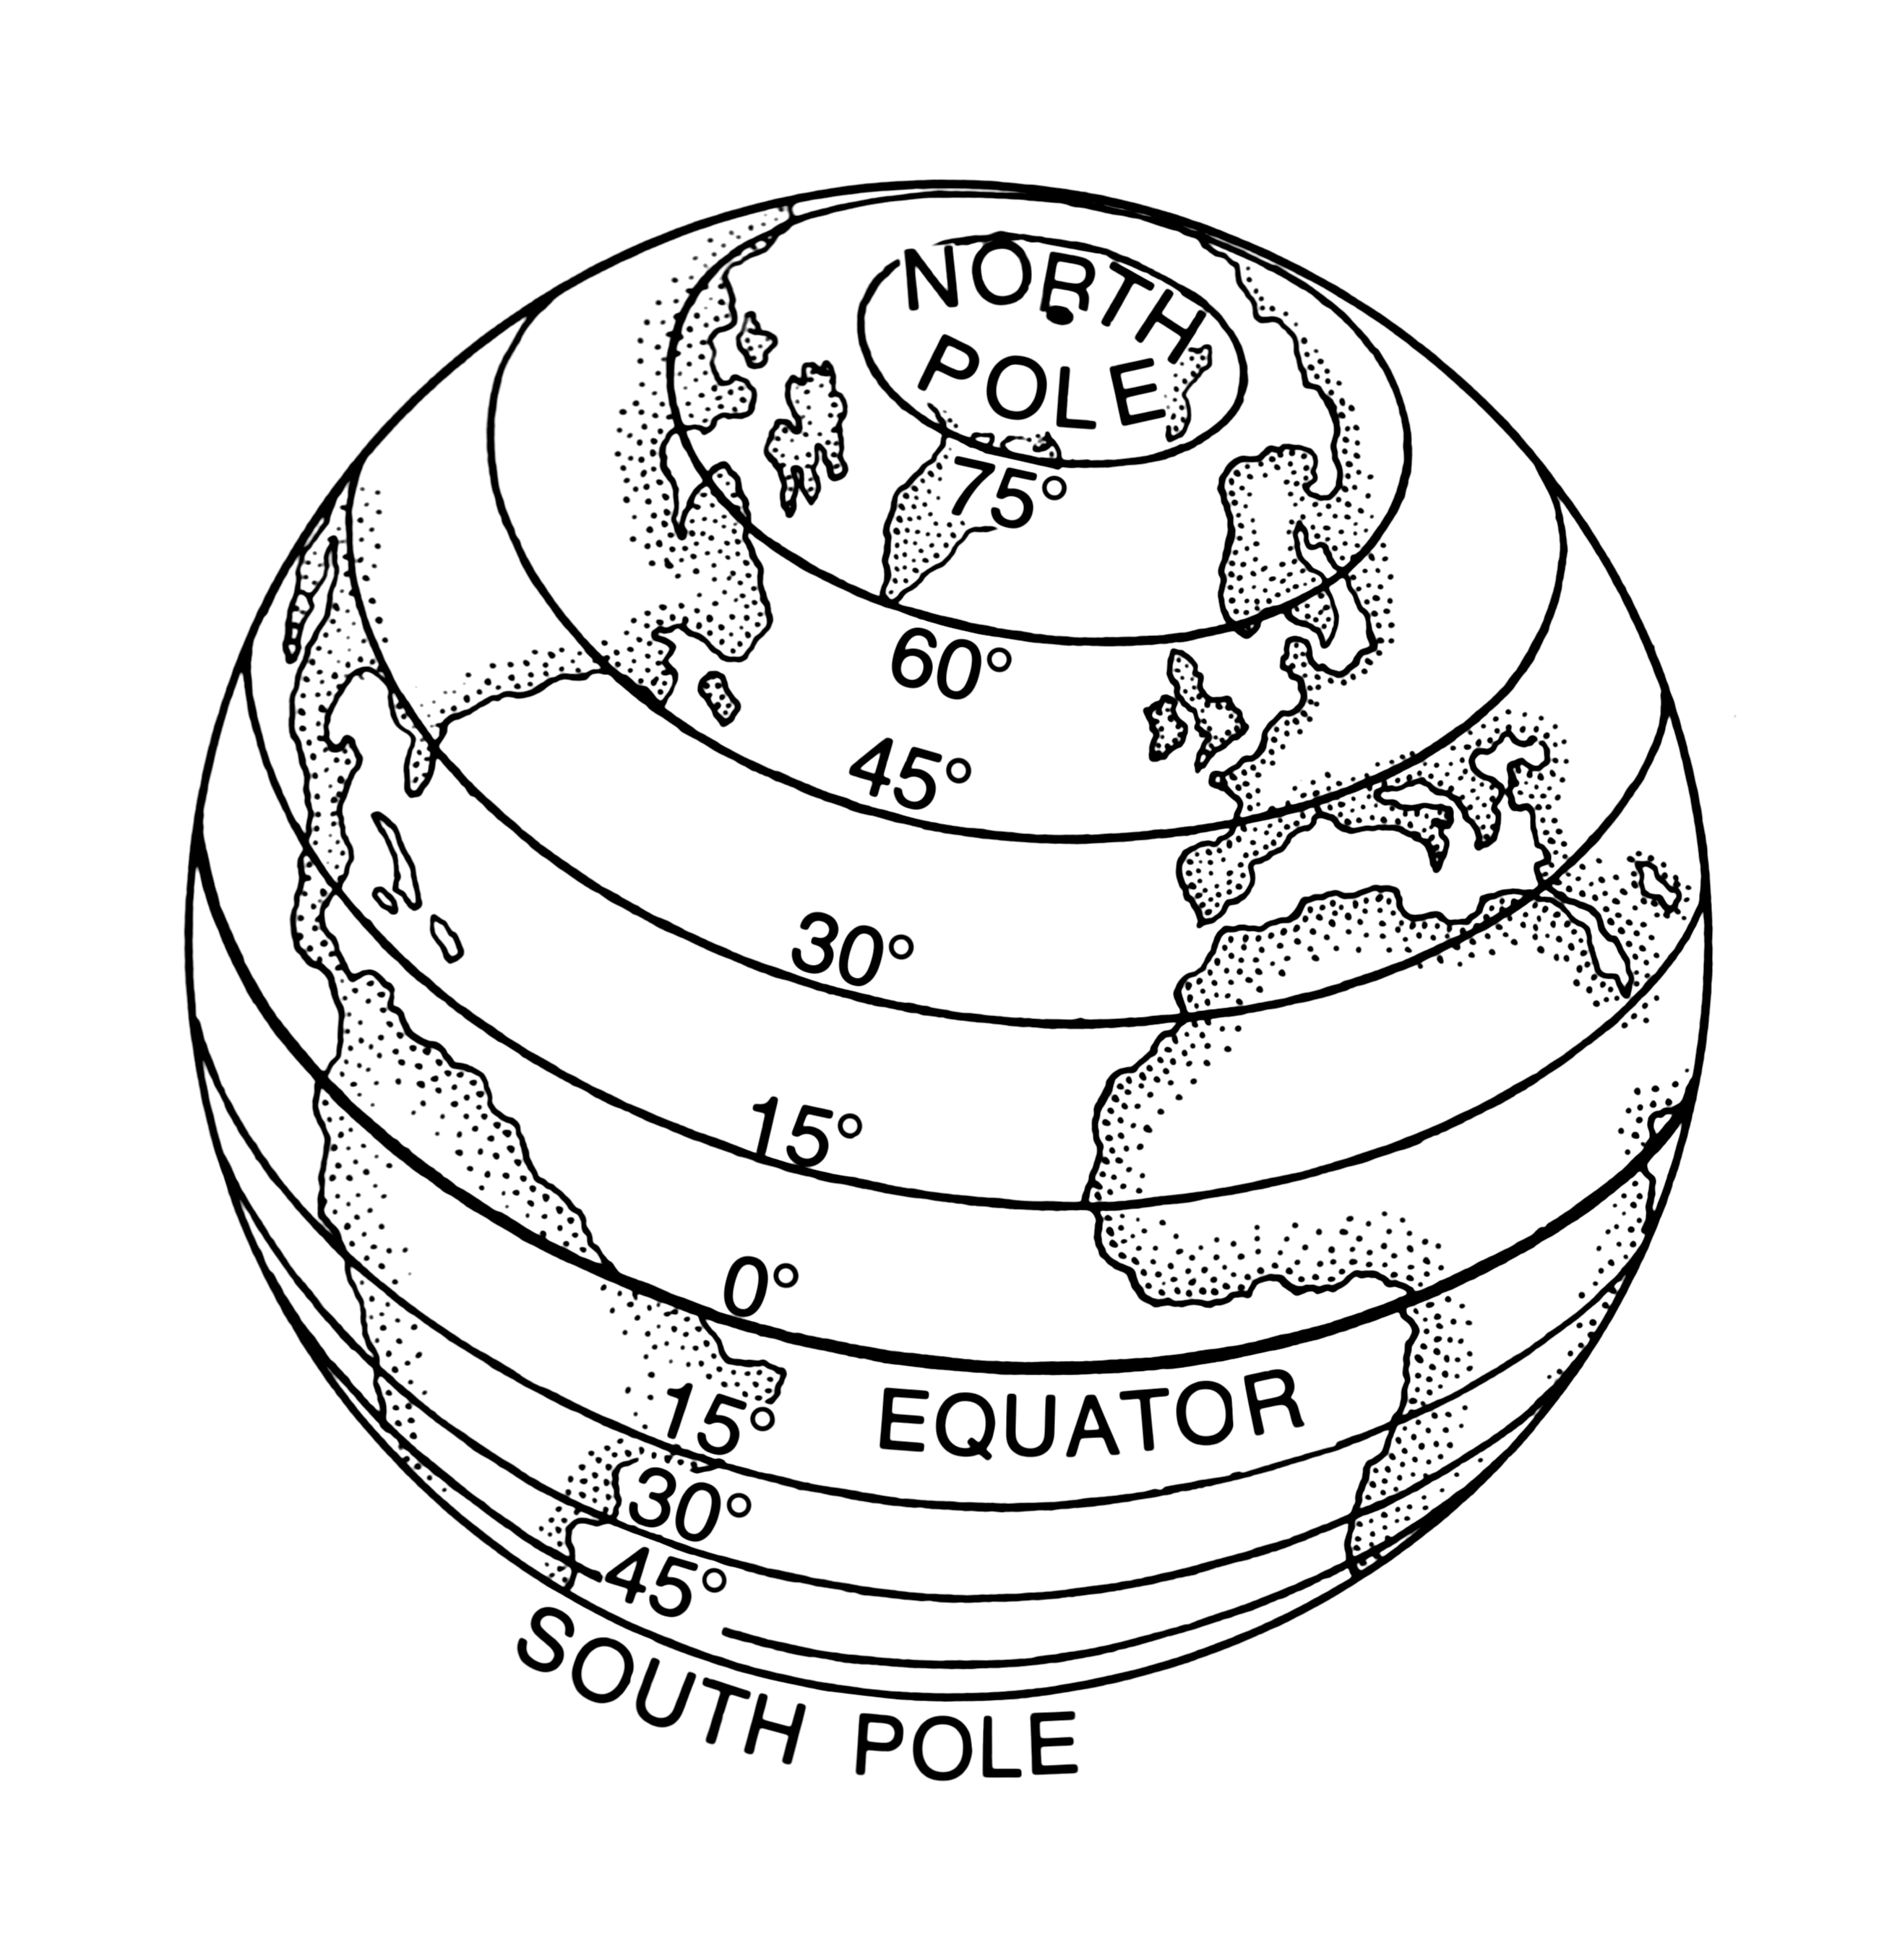
\includegraphics[width=2in]{./RadianMeasureGraphics/Latitude_(PSF).png}

\end{center}

\smallskip

{\bf Solution.}  To use the formula $v = r \omega$, we first need to compute the angular velocity $\omega$.  The earth makes one revolution in 24 hours, and one revolution is $2 \pi$ radians, so $\omega = \frac{2 \pi \, \text{radians}}{24 \, \text{hours}} = \frac{\pi}{12 \, \text{hours}}$. Note that once again, we are identifying angles in radian measure as real numbers so we can drop the `radian' units as they are dimensionless.  Also note that  for simplicity's sake, we assume that we are viewing the rotation of the earth as counter-clockwise so $\omega > 0$.  Hence, the linear velocity is \[ v = 2960 \, \text{miles} \cdot \frac{\pi}{12 \, \text{hours}} \approx 775 \, \frac{\text{miles}}{\text{hour}}\]  \qed

\end{ex}

It is worth noting that the quantity $\frac{1 \, \text{revolution}}{24 \, \text{hours}}$ in Example \ref{EarthRotationEx} is called the \index{frequency ! ordinary} \index{ordinary frequency} \textbf{ordinary frequency} of the motion and is usually denoted by the variable $f$.  The ordinary frequency is a measure of how often an object makes a complete cycle of the motion.  The fact that $\omega = 2\pi f$ suggests that $\omega$ is also a frequency.  Indeed, it is called the \index{frequency ! angular} \index{angular frequency} \textbf{angular frequency} of the motion.  On a related note, the quantity $T = \frac{1}{f}$ is called the \index{period ! circular motion}\textbf{period} of the motion and is the amount of time it takes for the object to complete one cycle of the motion.  In the scenario of Example \ref{EarthRotationEx}, the period of the motion is 24 hours, or one day.  

\smallskip

The concepts of frequency and period help frame the equation $v = r \omega$ in a new light.  That is, if $\omega$ is fixed, points which are farther from the center of rotation need to travel faster to maintain the same angular frequency since they have farther to travel to make one revolution in one period's time.  The distance of the object to the center of rotation is the radius of the circle, $r$, and is the `magnification factor' which relates $\omega$ and $v$. We will have more to say about frequencies and periods in Section \ref{GraphsofSineandCosine}.  While we have exhaustively discussed velocities associated with circular motion, we have yet to discuss a more natural question: if an object is moving on a circular path of radius $r$ with a fixed angular velocity (frequency) $\omega$, what is the position of the object at time $t$?  The answer to this question is the very heart of Trigonometry and is answered in the next section.   

\newpage

\subsection{Exercises}




In Exercises \ref{orientedanglefirst} - \ref{orientedanglelast}, graph the oriented angle in standard position. Classify each angle according to where its terminal side lies and then give two coterminal angles, one of which is positive and the other negative.


\begin{multicols}{4} 

\begin{enumerate}


\item $\dfrac{\pi}{3}$
\item $\dfrac{5\pi}{6}$
\item $-\dfrac{11\pi}{3}$
\item $\dfrac{5\pi}{4}$

\setcounter{HW}{\value{enumi}}

\end{enumerate}

\end{multicols}

\begin{multicols}{4} 

\begin{enumerate}

\setcounter{enumi}{\value{HW}}

\item $\dfrac{3\pi}{4}$
\item $-\dfrac{\pi}{3}$ \vphantom{$\dfrac{11\pi}{6}$}
\item $\dfrac{7\pi}{2}$
\item $\dfrac{\pi}{4}$ \vphantom{$\dfrac{11\pi}{6}$}

\setcounter{HW}{\value{enumi}}

\end{enumerate}

\end{multicols}

\begin{multicols}{4} 

\begin{enumerate}

\setcounter{enumi}{\value{HW}}

\item $-\dfrac{\pi}{2}$ \vphantom{$\dfrac{11\pi}{6}$}
\item $\dfrac{7\pi}{6}$
\item $-\dfrac{5\pi}{3}$
\item $3\pi$ \vphantom{$\dfrac{11\pi}{6}$}

\setcounter{HW}{\value{enumi}}

\end{enumerate}

\end{multicols}

\begin{multicols}{4} 

\begin{enumerate}

\setcounter{enumi}{\value{HW}}

\item  $-2\pi$ \vphantom{$\dfrac{11\pi}{6}$}
\item $-\dfrac{\pi}{4}$ \vphantom{$\dfrac{11\pi}{6}$}
\item $\dfrac{15\pi}{4}$
\item $-\dfrac{13\pi}{6}$ \label{orientedanglelast}

\setcounter{HW}{\value{enumi}}

\end{enumerate}

\end{multicols}

In Exercises \ref{degreetoradianfirst} - \ref{degreetoradianlast}, convert the angle from degree measure into radian measure, giving the exact value in terms of $\pi$.

\begin{multicols}{4} 

\begin{enumerate}

\setcounter{enumi}{\value{HW}}

\item $0^{\circ}$ \label{degreetoradianfirst}
\item $240^{\circ}$
\item $135^{\circ}$
\item $-270^{\circ}$

\setcounter{HW}{\value{enumi}}

\end{enumerate}

\end{multicols}

\begin{multicols}{4} 

\begin{enumerate}

\setcounter{enumi}{\value{HW}}

\item $-315^{\circ}$
\item $150^{\circ}$
\item $45^{\circ}$
\item $-225^{\circ}$ \label{degreetoradianlast}

\setcounter{HW}{\value{enumi}}

\end{enumerate}

\end{multicols}

In Exercises \ref{radiantodegreefirst} - \ref{radiantodegreelast}, convert the angle from radian measure into degree measure.

\begin{multicols}{4} 

\begin{enumerate}

\setcounter{enumi}{\value{HW}}

\item $\pi$ \vphantom{$\dfrac{11\pi}{6}$} \label{radiantodegreefirst}
\item $-\dfrac{2\pi}{3}$
\item $\dfrac{7\pi}{6}$
\item $\dfrac{11\pi}{6}$

\setcounter{HW}{\value{enumi}}

\end{enumerate}

\end{multicols}

\begin{multicols}{4} 

\begin{enumerate}

\setcounter{enumi}{\value{HW}}

\item $\dfrac{\pi}{3}$ \vphantom{$\dfrac{11\pi}{6}$}
\item $\dfrac{5\pi}{3}$
\item $-\dfrac{\pi}{6}$ \vphantom{$\dfrac{11\pi}{6}$}
\item $\dfrac{\pi}{2}$ \vphantom{$\dfrac{11\pi}{6}$} \label{radiantodegreelast}

\setcounter{HW}{\value{enumi}}

\end{enumerate}

\end{multicols}


In Exercises \ref{orientedarcfirst} - \ref{orientedarclast}, sketch the oriented arc on the Unit Circle which  corresponds to the given real number. 

\begin{multicols}{5} 

\begin{enumerate}

\setcounter{enumi}{\value{HW}}

\item $t=\frac{5 \pi}{6}$ \label{orientedarcfirst}

\item $t=-\pi$

\item $t = 6$

\item  $t = -2$

\item  $t = 12$ \label{orientedarclast}

\setcounter{HW}{\value{enumi}}

\end{enumerate}

\end{multicols}

\begin{enumerate}

\setcounter{enumi}{\value{HW}}

\item  \label{spinningyoyo} A yo-yo which is 2.25 inches in diameter spins at a rate of 4500 revolutions per minute.  How fast is the edge of the yo-yo spinning in miles per hour?  Round your answer to two decimal places.

\item  How many revolutions per minute would the yo-yo in exercise \ref{spinningyoyo} have to complete if the edge of the yo-yo is to be spinning at a rate of 42 miles per hour?  Round your answer to two decimal places.

\item  \label{yoyotrick} In the yo-yo trick `Around the World,' the performer throws the yo-yo so it sweeps out a vertical circle whose radius is the yo-yo string. If the yo-yo string is 28 inches long and the yo-yo takes 3 seconds to complete one revolution of the circle, compute the speed of the yo-yo in miles per hour.  Round your answer to two decimal places.

\item A computer hard drive contains a circular disk with diameter 2.5 inches and spins at a rate of 7200 revolutions per minute.  Find the linear speed of a point on the edge of the disk in miles per hour. \label{harddrive} 

\item A rock got stuck in the tread of my tire and when I was driving 70 miles per hour, the rock came loose and hit the inside of the wheel well of the car.  How fast, in miles per hour, was the rock traveling when it came out of the tread?  (The tire has a diameter of 23 inches.)

\item The Giant Wheel at Cedar Point is a circle with diameter 128 feet which sits on an 8 foot tall platform making its overall height is 136 feet.  (Remember this from Exercise \ref{giantwheelcircle} in Section \ref{Circles}?)  It completes two revolutions in 2 minutes and 7 seconds.\footnote{Source: \href{http://www.cedarpoint.com/public/park/rides/tranquil/giant_wheel.cfm}{\underline{Cedar Point's webpage}}.}  Assuming the riders are at the edge of the circle, how fast are they traveling in miles per hour?
\label{giantwheelmotion}

\item  Consider the circle of radius $r$ pictured below with central angle $\theta$, measured in radians,  and subtended arc of length $s$.  Prove that the area of the shaded sector is $A = \frac{1}{2} r^{2} \theta$. 

(Hint: Use the proportion  $\frac{A}{\text{area of the circle}} = \frac{s}{\text{circumference of the circle}}$.)
\label{circularsectorarea}

\begin{center}

\begin{mfpic}[20]{-5}{5}{-5}{5}
 \drawcolor[gray]{0.7}
\circle{(0,0),3}
\fillcolor[gray]{0.7}
\gfill \plrregion{0,60,5}{3}
\drawcolor{black}
\polyline{(3, 0), (0,0), (1.5, 2.598)}
\arrow \reverse \arrow \parafcn{5, 55, 5}{1.5*dir(t)}
\point[4pt]{(0,0)}
\tlabel[cc](1.732, 1){$\theta$}
\penwd{1.5pt}
\parafcn{0,60,5}{3*dir(t)}
\tlabel[cc](3.0311,1.75){$s$}
\tlabel[cc](1.5,-0.5){$r$}
\tlabel[cc](0.5,1.5){$r$}
\end{mfpic}

\end{center}

\setcounter{HW}{\value{enumi}}

\end{enumerate}

In Exercises \ref{sectorfirst} - \ref{sectorlast}, use the result of Exercise \ref{circularsectorarea} to compute the areas of the circular sectors with the given central angles and radii.

\begin{multicols}{3} 

\begin{enumerate}

\setcounter{enumi}{\value{HW}}

\item $\theta = \dfrac{\pi}{6}, \; r = 12$ \vphantom{$\dfrac{5\pi}{4}$} \label{sectorfirst}
\item $\theta = \dfrac{5\pi}{4}, \; r = 100$
\item $\theta = 330^{\circ}, \; r = 9.3$ \vphantom{$\dfrac{5\pi}{4}$}

\setcounter{HW}{\value{enumi}}

\end{enumerate}

\end{multicols}

\begin{multicols}{3} 

\begin{enumerate}

\setcounter{enumi}{\value{HW}}

\item $\theta =\pi, \; r = 1$
\item $\theta = 240^{\circ}, \; r = 5$
\item $\theta = 1^{\circ}, \; r = 117$ \label{sectorlast}

\setcounter{HW}{\value{enumi}}

\end{enumerate}

\end{multicols}

\begin{enumerate}

\setcounter{enumi}{\value{HW}}

\item Imagine a rope tied around the Earth at the equator.  Show that you need to add only $2\pi$ feet of length to the rope in order to lift it one foot above the ground around the entire equator.  (You do NOT need to know the radius of the Earth to show this.)

\item With the help of your classmates, look for a proof that $\pi$ is indeed a constant.

\end{enumerate}

\newpage

\subsection{Answers}


\begin{multicols}{2} \raggedcolumns

\begin{enumerate}


\item $\dfrac{\pi}{3}$  is a Quadrant I angle\\
coterminal with $\dfrac{7\pi}{3}$ and $-\dfrac{5\pi}{3}$ 

\begin{mfpic}[12]{-5}{5}{-5}{5}
\drawcolor[gray]{0.7}
\axes
\xmarks{-4,-3,-2,-1,1,2,3,4}
\ymarks{-4,-3,-2,-1,1,2,3,4}
\tlabel(5,-0.5){\scriptsize $x$}
\tlabel(0.25,4.75){\scriptsize $y$}
\drawcolor{black}
\arrow \arc[c]{(0,0), (2.5,-0.1), 55}
\penwd{1.25pt}
\arrow \reverse \arrow \polyline{(2.5, 4.3301), (0,0), (5,0)}
\point[4pt]{(0,0)}
\tlpointsep{5pt}
\scriptsize
\axislabels {x}{{$-4 \hspace{7pt}$} -4, {$-3 \hspace{7pt}$} -3, {$-2 \hspace{7pt}$} -2, {$-1 \hspace{7pt}$} -1, {$1$} 1, {$2$} 2, {$3$} 3, {$4$} 4}
\axislabels {y}{{$-1$} -1, {$-2$} -2, {$-3$} -3, {$-4$} -4, {$1$} 1, {$2$} 2, {$3$} 3, {$4$} 4}
\normalsize
\end{mfpic}

\item $\dfrac{5\pi}{6}$ is a Quadrant II angle\\
coterminal with $\dfrac{17\pi}{6}$ and $-\dfrac{7\pi}{6}$

\begin{mfpic}[12]{-5}{5}{-5}{5}
\drawcolor[gray]{0.7}
\axes
\xmarks{-4,-3,-2,-1,1,2,3,4}
\ymarks{-4,-3,-2,-1,1,2,3,4}
\tlabel(5,-0.5){\scriptsize $x$}
\tlabel(0.25,4.75){\scriptsize $y$}
\drawcolor{black}
\arrow \arc[c]{(0,0), (2.5,0.1), 145}
\penwd{1.25pt}
\arrow \reverse \arrow \polyline{(-4.3301, 2.5), (0,0), (5,0)}
\point[4pt]{(0,0)}
\tlpointsep{5pt}
\scriptsize
\axislabels {x}{{$-4 \hspace{7pt}$} -4, {$-3 \hspace{7pt}$} -3, {$-2 \hspace{7pt}$} -2, {$-1 \hspace{7pt}$} -1, {$1$} 1, {$2$} 2, {$3$} 3, {$4$} 4}
\axislabels {y}{{$-1$} -1, {$-2$} -2, {$-3$} -3, {$-4$} -4, {$1$} 1, {$2$} 2, {$3$} 3, {$4$} 4}
\normalsize
\end{mfpic}

\setcounter{HW}{\value{enumi}}

\end{enumerate}

\end{multicols}

\begin{multicols}{2} \raggedcolumns

\begin{enumerate}

\setcounter{enumi}{\value{HW}}

\item $-\dfrac{11\pi}{3}$ \vphantom{$\dfrac{17\pi}{6}$} is a Quadrant I angle\\
coterminal with $\dfrac{\pi}{3}$ and $-\dfrac{5\pi}{3}$ \vphantom{$\dfrac{17\pi}{4}$}

\begin{mfpic}[12]{-5}{5}{-5}{5}
\drawcolor[gray]{0.7}
\axes
\xmarks{-4,-3,-2,-1,1,2,3,4}
\ymarks{-4,-3,-2,-1,1,2,3,4}
\tlabel(5,-0.5){\scriptsize $x$}
\tlabel(0.25,4.75){\scriptsize $y$}
\drawcolor{black}
\arrow \parafcn{0,655,5}{(t+100)*dir(0-t)/400}
\penwd{1.25pt}
\arrow \reverse \arrow \polyline{(2.5, 4.3301), (0,0), (5,0)}
\point[4pt]{(0,0)}
\tlpointsep{5pt}
\scriptsize
\axislabels {x}{{$-4 \hspace{7pt}$} -4, {$-3 \hspace{7pt}$} -3, {$-2 \hspace{7pt}$} -2, {$-1 \hspace{7pt}$} -1, {$1$} 1, {$2$} 2, {$3$} 3, {$4$} 4}
\axislabels {y}{{$-1$} -1, {$-2$} -2, {$-3$} -3, {$-4$} -4, {$1$} 1, {$2$} 2, {$3$} 3, {$4$} 4}
\normalsize
\end{mfpic} 

\item $\dfrac{5\pi}{4}$ is a Quadrant III angle\\
coterminal with $\dfrac{13\pi}{4}$ and $-\dfrac{3\pi}{4}$

\begin{mfpic}[12]{-5}{5}{-5}{5}
\drawcolor[gray]{0.7}
\axes
\xmarks{-4,-3,-2,-1,1,2,3,4}
\ymarks{-4,-3,-2,-1,1,2,3,4}
\tlabel(5,-0.5){\scriptsize $x$}
\tlabel(0.25,4.75){\scriptsize $y$}
\drawcolor{black}
\arrow \arc[c]{(0,0), (2.5,0.1), 220}
\penwd{1.25pt}
\arrow \reverse \arrow \polyline{(-3.5355, -3.5355), (0,0), (5,0)}
\point[4pt]{(0,0)}
\tlpointsep{5pt}
\scriptsize
\axislabels {x}{{$-4 \hspace{7pt}$} -4, {$-3 \hspace{7pt}$} -3, {$-2 \hspace{7pt}$} -2, {$-1 \hspace{7pt}$} -1, {$1$} 1, {$2$} 2, {$3$} 3, {$4$} 4}
\axislabels {y}{{$-1$} -1, {$-2$} -2, {$-3$} -3, {$-4$} -4, {$1$} 1, {$2$} 2, {$3$} 3, {$4$} 4}
\normalsize
\end{mfpic}

\setcounter{HW}{\value{enumi}}

\end{enumerate}

\end{multicols}

\begin{multicols}{2} \raggedcolumns

\begin{enumerate}

\setcounter{enumi}{\value{HW}}

\item $\dfrac{3\pi}{4}$ is a Quadrant II angle\\
coterminal with $\dfrac{11\pi}{4}$ and $-\dfrac{5\pi}{4}$

\begin{mfpic}[12]{-5}{5}{-5}{5}
\drawcolor[gray]{0.7}
\axes
\xmarks{-4,-3,-2,-1,1,2,3,4}
\ymarks{-4,-3,-2,-1,1,2,3,4}
\tlabel(5,-0.5){\scriptsize $x$}
\tlabel(0.25,4.75){\scriptsize $y$}
\drawcolor{black}
\arrow \arc[c]{(0,0), (2.5,0.1), 130}
\penwd{1.25pt}
\arrow \reverse \arrow \polyline{(-3.5355, 3.5355), (0,0), (5,0)}
\point[4pt]{(0,0)}
\tlpointsep{5pt}
\scriptsize
\axislabels {x}{{$-4 \hspace{7pt}$} -4, {$-3 \hspace{7pt}$} -3, {$-2 \hspace{7pt}$} -2, {$-1 \hspace{7pt}$} -1, {$1$} 1, {$2$} 2, {$3$} 3, {$4$} 4}
\axislabels {y}{{$-1$} -1, {$-2$} -2, {$-3$} -3, {$-4$} -4, {$1$} 1, {$2$} 2, {$3$} 3, {$4$} 4}
\normalsize
\end{mfpic}

\item $-\dfrac{\pi}{3}$ \vphantom{$\dfrac{17\pi}{4}$} is a Quadrant IV angle\\
coterminal with $\dfrac{5\pi}{3}$ and $-\dfrac{7\pi}{3}$ \vphantom{$\dfrac{17\pi}{4}$}

\begin{mfpic}[12]{-5}{5}{-5}{5}
\drawcolor[gray]{0.7}
\axes
\xmarks{-4,-3,-2,-1,1,2,3,4}
\ymarks{-4,-3,-2,-1,1,2,3,4}
\tlabel(5,-0.5){\scriptsize $x$}
\tlabel(0.25,4.75){\scriptsize $y$}
\drawcolor{black}
\arrow \arc[c]{(0,0), (2.5,-0.1), -55}
\penwd{1.25pt}
\arrow \reverse \arrow \polyline{(2.5, -4.3301), (0,0), (5,0)}
\point[4pt]{(0,0)}
\tlpointsep{5pt}
\scriptsize
\axislabels {x}{{$-4 \hspace{7pt}$} -4, {$-3 \hspace{7pt}$} -3, {$-2 \hspace{7pt}$} -2, {$-1 \hspace{7pt}$} -1, {$1$} 1, {$2$} 2, {$3$} 3, {$4$} 4}
\axislabels {y}{{$-1$} -1, {$-2$} -2, {$-3$} -3, {$-4$} -4, {$1$} 1, {$2$} 2, {$3$} 3, {$4$} 4}
\normalsize
\end{mfpic}

\setcounter{HW}{\value{enumi}}

\end{enumerate}

\end{multicols}

\begin{multicols}{2} \raggedcolumns

\begin{enumerate}

\setcounter{enumi}{\value{HW}}

\item $\dfrac{7\pi}{2}$ lies on the negative $y$-axis \vphantom{$\dfrac{17\pi}{4}$}\\
coterminal with $\dfrac{3\pi}{2}$ and $-\dfrac{\pi}{2}$ \vphantom{$\dfrac{17\pi}{4}$}

\begin{mfpic}[12]{-5}{5}{-5}{5}
\drawcolor[gray]{0.7}
\axes
\xmarks{-4,-3,-2,-1,1,2,3,4}
\ymarks{-4,-3,-2,-1,1,2,3,4}
\tlabel(5,-0.5){\scriptsize $x$}
\tlabel(0.25,4.75){\scriptsize $y$}
\drawcolor{black}
\arrow \parafcn{0,625,5}{(t+100)*dir(t)/400}
\penwd{1.25pt}
\arrow \reverse \arrow \polyline{(0, -5), (0,0), (5,0)}
\point[4pt]{(0,0)}
\tlpointsep{5pt}
\scriptsize
\axislabels {x}{{$-4 \hspace{7pt}$} -4, {$-3 \hspace{7pt}$} -3, {$-2 \hspace{7pt}$} -2, {$-1 \hspace{7pt}$} -1, {$1$} 1, {$2$} 2, {$3$} 3, {$4$} 4}
\axislabels {y}{{$-1$} -1, {$-2$} -2, {$-3$} -3, {$-4$} -4, {$1$} 1, {$2$} 2, {$3$} 3, {$4$} 4}
\normalsize
\end{mfpic} 

\item $\dfrac{\pi}{4}$ is a Quadrant I angle \vphantom{$\dfrac{17\pi}{2}$}\\
coterminal with $\dfrac{9 \pi}{4}$ and $-\dfrac{7\pi}{4}$

\begin{mfpic}[12]{-5}{5}{-5}{5}
\drawcolor[gray]{0.7}
\axes
\xmarks{-4,-3,-2,-1,1,2,3,4}
\ymarks{-4,-3,-2,-1,1,2,3,4}
\tlabel(5,-0.5){\scriptsize $x$}
\tlabel(0.25,4.75){\scriptsize $y$}
\drawcolor{black}
\arrow \arc[c]{(0,0), (2.5, 0.1), 40}
\penwd{1.25pt}
\arrow \reverse \arrow \polyline{(3.5355, 3.5355), (0,0), (5,0)}
\point[4pt]{(0,0)}
\tlpointsep{5pt}
\scriptsize
\axislabels {x}{{$-4 \hspace{7pt}$} -4, {$-3 \hspace{7pt}$} -3, {$-2 \hspace{7pt}$} -2, {$-1 \hspace{7pt}$} -1, {$1$} 1, {$2$} 2, {$3$} 3, {$4$} 4}
\axislabels {y}{{$-1$} -1, {$-2$} -2, {$-3$} -3, {$-4$} -4, {$1$} 1, {$2$} 2, {$3$} 3, {$4$} 4}
\normalsize
\end{mfpic}

\setcounter{HW}{\value{enumi}}

\end{enumerate}

\end{multicols}

\begin{multicols}{2} \raggedcolumns

\begin{enumerate}

\setcounter{enumi}{\value{HW}}

\item $-\dfrac{\pi}{2}$ lies on the negative $y$-axis \vphantom{$\dfrac{17\pi}{4}$}\\
coterminal with $\dfrac{3\pi}{2}$ and $-\dfrac{5\pi}{2}$

\begin{mfpic}[12]{-5}{5}{-5}{5}
\drawcolor[gray]{0.7}
\axes
\xmarks{-4,-3,-2,-1,1,2,3,4}
\ymarks{-4,-3,-2,-1,1,2,3,4}
\tlabel(5,-0.5){\scriptsize $x$}
\tlabel(0.25,4.75){\scriptsize $y$}
\drawcolor{black}
\arrow \arc[c]{(0,0), (2.5, -0.1), -85}
\penwd{1.25pt}
 \arrow \reverse \arrow \polyline{(0, -5), (0,0), (5,0)}
\point[4pt]{(0,0)}
\tlpointsep{5pt}
\scriptsize
\axislabels {x}{{$-4 \hspace{7pt}$} -4, {$-3 \hspace{7pt}$} -3, {$-2 \hspace{7pt}$} -2, {$-1 \hspace{7pt}$} -1, {$1$} 1, {$2$} 2, {$3$} 3, {$4$} 4}
\axislabels {y}{{$-1$} -1, {$-2$} -2, {$-3$} -3, {$-4$} -4, {$1$} 1, {$2$} 2, {$3$} 3, {$4$} 4}
\normalsize
\end{mfpic}

\item $\dfrac{7\pi}{6}$ is a Quadrant III angle\\
coterminal with $\dfrac{19 \pi}{6}$ and $-\dfrac{5\pi}{6}$

\begin{mfpic}[12]{-5}{5}{-5}{5}
\drawcolor[gray]{0.7}
\axes
\xmarks{-4,-3,-2,-1,1,2,3,4}
\ymarks{-4,-3,-2,-1,1,2,3,4}
\tlabel(5,-0.5){\scriptsize $x$}
\tlabel(0.25,4.75){\scriptsize $y$}
\drawcolor{black}
\arrow \arc[c]{(0,0), (2.5, 0.1), 205}
\penwd{1.25pt}
\arrow \reverse \arrow \polyline{(-4.3301,-2.5), (0,0), (5,0)}
\point[4pt]{(0,0)}
\tlpointsep{5pt}
\scriptsize
\axislabels {x}{{$-4 \hspace{7pt}$} -4, {$-3 \hspace{7pt}$} -3, {$-2 \hspace{7pt}$} -2, {$-1 \hspace{7pt}$} -1, {$1$} 1, {$2$} 2, {$3$} 3, {$4$} 4}
\axislabels {y}{{$-1$} -1, {$-2$} -2, {$-3$} -3, {$-4$} -4, {$1$} 1, {$2$} 2, {$3$} 3, {$4$} 4}
\normalsize
\end{mfpic}

\setcounter{HW}{\value{enumi}}

\end{enumerate}

\end{multicols}

\begin{multicols}{2} \raggedcolumns

\begin{enumerate}

\setcounter{enumi}{\value{HW}}

\item $-\dfrac{5\pi}{3}$ is a Quadrant I angle \vphantom{$\dfrac{17\pi}{4}$} \\
coterminal with $\dfrac{\pi}{3}$ and $-\dfrac{11\pi}{3}$ \vphantom{$\dfrac{17\pi}{4}$}

\begin{mfpic}[12]{-5}{5}{-5}{5}
\drawcolor[gray]{0.7}
\axes
\xmarks{-4,-3,-2,-1,1,2,3,4}
\ymarks{-4,-3,-2,-1,1,2,3,4}
\tlabel(5,-0.5){\scriptsize $x$}
\tlabel(0.25,4.75){\scriptsize $y$}
\drawcolor{black}
\arrow \arc[c]{(0,0), (2.5, -0.1), -295}
\penwd{1.25pt}
\arrow \reverse \arrow \polyline{(2.5, 4.3301), (0,0), (5,0)}
\point[4pt]{(0,0)}
\tlpointsep{5pt}
\scriptsize
\axislabels {x}{{$-4 \hspace{7pt}$} -4, {$-3 \hspace{7pt}$} -3, {$-2 \hspace{7pt}$} -2, {$-1 \hspace{7pt}$} -1, {$1$} 1, {$2$} 2, {$3$} 3, {$4$} 4}
\axislabels {y}{{$-1$} -1, {$-2$} -2, {$-3$} -3, {$-4$} -4, {$1$} 1, {$2$} 2, {$3$} 3, {$4$} 4}
\normalsize
\end{mfpic}

\item $3\pi$ lies on the negative $x$-axis \vphantom{$\dfrac{17\pi}{4}$} \\
coterminal with $\pi$ and $-\pi$ \vphantom{$\dfrac{17\pi}{4}$}

\begin{mfpic}[12]{-5}{5}{-5}{5}
\drawcolor[gray]{0.7}
\axes
\xmarks{-4,-3,-2,-1,1,2,3,4}
\ymarks{-4,-3,-2,-1,1,2,3,4}
\tlabel(5,-0.5){\scriptsize $x$}
\tlabel(0.25,4.75){\scriptsize $y$}
\drawcolor{black}
\arrow \parafcn{0,535,5}{(t+100)*dir(t)/400}
\penwd{1.25pt}
\arrow \reverse \arrow \polyline{(-5,0), (0,0), (5,0)}
\point[4pt]{(0,0)}
\tlpointsep{5pt}
\scriptsize
\axislabels {x}{{$-4 \hspace{7pt}$} -4, {$-3 \hspace{7pt}$} -3, {$-2 \hspace{7pt}$} -2, {$-1 \hspace{7pt}$} -1, {$1$} 1, {$2$} 2, {$3$} 3, {$4$} 4}
\axislabels {y}{{$-1$} -1, {$-2$} -2, {$-3$} -3, {$-4$} -4, {$1$} 1, {$2$} 2, {$3$} 3, {$4$} 4}
\normalsize
\end{mfpic} 

\setcounter{HW}{\value{enumi}}

\end{enumerate}

\end{multicols}

\begin{multicols}{2} \raggedcolumns

\begin{enumerate}

\setcounter{enumi}{\value{HW}}

\item $-2\pi$ lies on the positive $x$-axis \vphantom{$\dfrac{17\pi}{4}$} \\
coterminal with $2\pi$ and $-4\pi$ \vphantom{$\dfrac{17\pi}{4}$}

\begin{mfpic}[12]{-5}{5}{-5}{5}
\drawcolor[gray]{0.7}
\axes
\xmarks{-4,-3,-2,-1,1,2,3,4}
\ymarks{-4,-3,-2,-1,1,2,3,4}
\tlabel(5,-0.5){\scriptsize $x$}
\tlabel(0.25,4.75){\scriptsize $y$}
\drawcolor{black}
\arrow \parafcn{0,355,5}{(t+100)*dir(0-t)/300}
\penwd{1.25pt}
\point[4pt]{(0,0)}
\arrow \polyline{(0,0), (5,0)}
\tlpointsep{5pt}
\scriptsize
\axislabels {x}{{$-4 \hspace{7pt}$} -4, {$-3 \hspace{7pt}$} -3, {$-2 \hspace{7pt}$} -2, {$-1 \hspace{7pt}$} -1, {$1$} 1, {$2$} 2, {$3$} 3, {$4$} 4}
\axislabels {y}{{$-1$} -1, {$-2$} -2, {$-3$} -3, {$-4$} -4, {$1$} 1, {$2$} 2, {$3$} 3, {$4$} 4}
\normalsize
\end{mfpic}

\item $-\dfrac{\pi}{4}$ is a Quadrant IV angle \vphantom{$\dfrac{17\pi}{4}$} \\
coterminal with $\dfrac{7 \pi}{4}$ and $-\dfrac{9\pi}{4}$

\begin{mfpic}[12]{-5}{5}{-5}{5}
\drawcolor[gray]{0.7}
\axes
\xmarks{-4,-3,-2,-1,1,2,3,4}
\ymarks{-4,-3,-2,-1,1,2,3,4}
\tlabel(5,-0.5){\scriptsize $x$}
\tlabel(0.25,4.75){\scriptsize $y$}
\drawcolor{black}
\arrow \arc[c]{(0,0), (2.5, -0.1), -40}
\penwd{1.25pt}
\arrow \reverse \arrow \polyline{(3.5355,-3.5355), (0,0), (5,0)}
\point[4pt]{(0,0)}
\tlpointsep{5pt}
\scriptsize
\axislabels {x}{{$-4 \hspace{7pt}$} -4, {$-3 \hspace{7pt}$} -3, {$-2 \hspace{7pt}$} -2, {$-1 \hspace{7pt}$} -1, {$1$} 1, {$2$} 2, {$3$} 3, {$4$} 4}
\axislabels {y}{{$-1$} -1, {$-2$} -2, {$-3$} -3, {$-4$} -4, {$1$} 1, {$2$} 2, {$3$} 3, {$4$} 4}
\normalsize
\end{mfpic}

\setcounter{HW}{\value{enumi}}

\end{enumerate}

\end{multicols}

\begin{multicols}{2} \raggedcolumns

\begin{enumerate}

\setcounter{enumi}{\value{HW}}

\item $\dfrac{15\pi}{4}$ is a Quadrant IV angle\\
coterminal with $\dfrac{7\pi}{4}$ and $-\dfrac{\pi}{4}$

\begin{mfpic}[12]{-5}{5}{-5}{5}
\drawcolor[gray]{0.7}
\axes
\xmarks{-4,-3,-2,-1,1,2,3,4}
\ymarks{-4,-3,-2,-1,1,2,3,4}
\tlabel(5,-0.5){\scriptsize $x$}
\tlabel(0.25,4.75){\scriptsize $y$}
\drawcolor{black}
\arrow \parafcn{0,670,5}{(t+100)*dir(t)/400}
\penwd{1.25pt}
\arrow \reverse \arrow \polyline{(3.5355,-3.5355), (0,0), (5,0)}
\point[4pt]{(0,0)}
\tlpointsep{5pt}
\scriptsize
\axislabels {x}{{$-4 \hspace{7pt}$} -4, {$-3 \hspace{7pt}$} -3, {$-2 \hspace{7pt}$} -2, {$-1 \hspace{7pt}$} -1, {$1$} 1, {$2$} 2, {$3$} 3, {$4$} 4}
\axislabels {y}{{$-1$} -1, {$-2$} -2, {$-3$} -3, {$-4$} -4, {$1$} 1, {$2$} 2, {$3$} 3, {$4$} 4}
\normalsize
\end{mfpic} 

\item $-\dfrac{13\pi}{6}$ is a Quadrant IV angle\\
coterminal with $\dfrac{11\pi}{6}$ and $-\dfrac{\pi}{6}$

\begin{mfpic}[12]{-5}{5}{-5}{5}
\drawcolor[gray]{0.7}
\axes
\xmarks{-4,-3,-2,-1,1,2,3,4}
\ymarks{-4,-3,-2,-1,1,2,3,4}
\tlabel(5,-0.5){\scriptsize $x$}
\tlabel(0.25,4.75){\scriptsize $y$}
\drawcolor{black}
\arrow \parafcn{0,385,5}{(t+100)*dir(0-t)/300}
\penwd{1.25pt}
\arrow \reverse \arrow \polyline{(4.3301,-2.5), (0,0), (5,0)}
\point[4pt]{(0,0)}
\tlpointsep{5pt}
\scriptsize
\axislabels {x}{{$-4 \hspace{7pt}$} -4, {$-3 \hspace{7pt}$} -3, {$-2 \hspace{7pt}$} -2, {$-1 \hspace{7pt}$} -1, {$1$} 1, {$2$} 2, {$3$} 3, {$4$} 4}
\axislabels {y}{{$-1$} -1, {$-2$} -2, {$-3$} -3, {$-4$} -4, {$1$} 1, {$2$} 2, {$3$} 3, {$4$} 4}
\normalsize
\end{mfpic} 

\setcounter{HW}{\value{enumi}}

\end{enumerate}

\end{multicols}

\begin{multicols}{4}

\begin{enumerate}

\setcounter{enumi}{\value{HW}}

\item $0$ \vphantom{$\dfrac{17\pi}{4}$}
\item $\dfrac{4\pi}{3}$
\item $\dfrac{3\pi}{4}$
\item $-\dfrac{3\pi}{2}$

\setcounter{HW}{\value{enumi}}

\end{enumerate}

\end{multicols}

\begin{multicols}{4}

\begin{enumerate}

\setcounter{enumi}{\value{HW}}

\item $-\dfrac{7\pi}{4}$
\item $\dfrac{5\pi}{6}$
\item $\dfrac{\pi}{4}$ \vphantom{$\dfrac{17\pi}{4}$}
\item $-\dfrac{5\pi}{4}$

\setcounter{HW}{\value{enumi}}

\end{enumerate}

\end{multicols}

\begin{multicols}{4}

\begin{enumerate}

\setcounter{enumi}{\value{HW}}

\item $180^{\circ}$
\item $-120^{\circ}$
\item $210^{\circ}$
\item $330^{\circ}$

\setcounter{HW}{\value{enumi}}

\end{enumerate}

\end{multicols}

\begin{multicols}{4}

\begin{enumerate}

\setcounter{enumi}{\value{HW}}

\item $60^{\circ}$
\item $300^{\circ}$
\item $-30^{\circ}$
\item $90^{\circ}$

\setcounter{HW}{\value{enumi}}

\end{enumerate}

\end{multicols}

\newpage

\begin{multicols}{2} \raggedcolumns

\begin{enumerate}

\setcounter{enumi}{\value{HW}}

\item  $t = \dfrac{5\pi}{6}$

\begin{mfpic}[10]{-5}{5}{-5}{5}
\axes
\tlabel(5,-0.5){\scriptsize $x$}
\tlabel(0.5,5){\scriptsize $y$}
\tlabel(3.1,-0.75){\scriptsize $1$}
\tlabel(0.25,3.1){\scriptsize $1$}
\xmarks{-3 step 3 until 3}
\ymarks{-3 step 3 until 3}
\dotted \polyline{(0,0), (-4.3301,2.5)}
\drawcolor[gray]{0.7}
\circle{(0,0),3}
\drawcolor{black}
\penwd{1.5pt}
\arrow \parafcn{0, 150, 5}{3*dir(t)}
\end{mfpic} 

\item  $t = -\pi$ \vphantom{$\dfrac{5\pi}{6}$}

\begin{mfpic}[10]{-5}{5}{-5}{5}
\axes
\tlabel(5,-0.5){\scriptsize $x$}
\tlabel(0.5,5){\scriptsize $y$}
\tlabel(3.1,-0.75){\scriptsize $1$}
\tlabel(0.25,3.1){\scriptsize $1$}
\xmarks{-3 step 3 until 3}
\ymarks{-3 step 3 until 3}
\drawcolor[gray]{0.7}
\circle{(0,0),3}
\drawcolor{black}
\penwd{1.5pt}
\arrow \parafcn{0, 180, 5}{3*dir(-t)}
\end{mfpic} 

\setcounter{HW}{\value{enumi}}

\end{enumerate}

\end{multicols}

\begin{multicols}{2} \raggedcolumns

\begin{enumerate}

\setcounter{enumi}{\value{HW}}

\item  $t = 6$

\begin{mfpic}[10]{-5}{5}{-5}{5}
\axes
\tlabel(5,-0.5){\scriptsize $x$}
\tlabel(0.5,5){\scriptsize $y$}
\tlabel(3.1,-0.75){\scriptsize $1$}
\tlabel(0.25,3.1){\scriptsize $1$}
\xmarks{-3 step 3 until 3}
\ymarks{-3 step 3 until 3}
\dotted \polyline{(0,0), (4.801,-1.397)}
\drawcolor[gray]{0.7}
\circle{(0,0),3}
\drawcolor{black}
\penwd{1.5pt}
\arrow \parafcn{0, 343, 5}{3*dir(t)}
\end{mfpic} 

\item  $t = -2$

\begin{mfpic}[10]{-5}{5}{-5}{5}
\axes
\tlabel(4.5,-0.5){\scriptsize $x$}
\tlabel(0.5,4.5){\scriptsize $y$}
\tlabel(3.1,-0.75){\scriptsize $1$}
\tlabel(0.25,3.1){\scriptsize $1$}
\xmarks{-3 step 3 until 3}
\ymarks{-3 step 3 until 3}
\dotted \polyline{(0,0), (-2.081,-4.546)}
\drawcolor[gray]{0.7}
\circle{(0,0),3}
\drawcolor{black}
\penwd{1.5pt}
\arrow \parafcn{0, 114, 5}{3*dir(-t)}
\end{mfpic} 

\setcounter{HW}{\value{enumi}}

\end{enumerate}

\end{multicols}

%\begin{multicols}{2} 

\begin{enumerate}

\setcounter{enumi}{\value{HW}}

\item  $t = 12$  (between 1 and 2 revolutions)

\begin{mfpic}[10]{-5}{5}{-5}{5}
\axes
\tlabel(5,-0.5){\scriptsize $x$}
\tlabel(0.5,5){\scriptsize $y$}
\tlabel(3.1,-0.75){\scriptsize $1$}
\tlabel(0.25,3.1){\scriptsize $1$}
\xmarks{-3 step 3 until 3}
\ymarks{-3 step 3 until 3}
\dotted \polyline{(0,0), (4.219,-2.683)}
\drawcolor[gray]{0.7}
\circle{(0,0),3}
\drawcolor{black}
\penwd{1.5pt}
\arrow \parafcn{0, 687, 5}{3*dir(t)}
\end{mfpic} 

\setcounter{HW}{\value{enumi}}

\end{enumerate}

%\end{multicols}

\begin{multicols}{2}

\begin{enumerate}

\setcounter{enumi}{\value{HW}}

\item About 30.12 miles per hour
\item About 6274.52 revolutions per minute

\setcounter{HW}{\value{enumi}}

\end{enumerate}

\end{multicols}

\begin{multicols}{2}

\begin{enumerate}

\setcounter{enumi}{\value{HW}}

\item About 3.33 miles per hour
\item About 53.55 miles per hour

\setcounter{HW}{\value{enumi}}

\end{enumerate}

\end{multicols}

\begin{multicols}{2}

\begin{enumerate}

\setcounter{enumi}{\value{HW}}

\item 70 miles per hour
\item About 4.32 miles per hour

\setcounter{HW}{\value{enumi}}

\end{enumerate}

\end{multicols}

\begin{multicols}{2}

\begin{enumerate}

\setcounter{enumi}{\value{HW}}

\addtocounter{enumi}{1}

\item $12\pi$ square units
\item $6250\pi$ square units 

\setcounter{HW}{\value{enumi}}

\end{enumerate}

\end{multicols}

\begin{multicols}{2}

\begin{enumerate}

\setcounter{enumi}{\value{HW}}

\item $79.2825\pi \approx 249.07$ square units \vphantom{$\dfrac{\pi}{2}$}
\item $\dfrac{\pi}{2}$ square units

\setcounter{HW}{\value{enumi}}

\end{enumerate}

\end{multicols}

\enlargethispage{0.25in}

\vspace{-0.25in}

\begin{multicols}{2}

\begin{enumerate}

\setcounter{enumi}{\value{HW}}

\item $\dfrac{50\pi}{3}$ square units
\item $38.025 \pi \approx 119.46$ square units \vphantom{$\dfrac{50\pi}{3}$}

\end{enumerate}

\end{multicols}





\closegraphsfile

\newpage

\section{The Circular Functions: Sine and Cosine}

\mfpicnumber{1}

\opengraphsfile{TheCircularFunctionsSineandCosine}

\setcounter{footnote}{0}

\label{TheCircularFunctionsSineandCosine}

In Section \ref{circularmotion}, we introduced circular motion and derived a formula which describes the linear velocity of an object moving on a circular path at a constant angular velocity.  One of the goals of this section is describe the \textit{position} of such an object.  To that end, consider an angle $\theta$ in standard position and let $P$ denote the point where the terminal side of $\theta$ intersects the Unit Circle, as diagrammed below.

\smallskip

\begin{tabular}{cc}

\begin{mfpic}[20]{-5}{5}{-5}{5}
\axes
\tlabel(4.75,-0.5){\scriptsize $x$}
\tlabel(0.25,5){\scriptsize $y$}
\tlabel(3.1,-0.75){\scriptsize $1$}
\tlabel(0.25,3.1){\scriptsize $1$}
\xmarks{-3 step 3 until 3}
\ymarks{-3 step 3 until 3}
\point[4pt]{(0,0)}
\drawcolor[gray]{0.7}
\circle{(0,0),3}
\drawcolor{black}
\arrow \parafcn{5, 55, 5}{1.5*dir(t)}
\penwd{1.25pt}
\arrow \reverse \arrow \polyline{(5,0),(0,0), (2.5, 4.3301)}

\tlabel[cc](1.9, 1){$\theta$}
\end{mfpic} 

&

\hspace{.25in}

\begin{mfpic}[20]{-5}{5}{-5}{5}
\axes
\tlabel(4.75,-0.5){\scriptsize $x$}
\tlabel(0.25,5){\scriptsize $y$}
\tlabel(3.1,-0.75){\scriptsize $1$}
\tlabel(0.25,3.1){\scriptsize $1$}
\xmarks{-3 step 3 until 3}
\ymarks{-3 step 3 until 3}
\arrow \reverse \arrow \polyline{(5,0),(0,0), (2.5, 4.3301)}
\tlabel(2,2.6){$P(\cos(\theta), \sin(\theta))$}
\drawcolor[gray]{0.7}
\circle{(0,0),3}
\drawcolor{black}
\arrow \parafcn{5, 55, 5}{1.5*dir(t)}
\penwd{1.25pt}
\arrow \reverse \arrow \polyline{(5,0),(0,0), (2.5, 4.3301)}
\tlabel[cc](1.9, 1){$\theta$}
\point[4pt]{(0,0), (1.5, 2.5981)}
\end{mfpic} 

\end{tabular}

\smallskip

 By associating the point $P$ with the angle $\theta$, we are assigning a \emph{position} on the Unit Circle to the angle $\theta$.  Since for each angle $\theta$, the terminal side of $\theta$, when graphed in standard position, intersects The Unit Circle only once, the mapping of $\theta$ to $P$ is a function.\footnote{See Definition \ref{functiondefn} in Section \ref{FunctionsandtheirRepresentations}.}   Since there is only \textit{one} way to describe a point using rectangular coordinates,\footnote{See page \pageref{importantfactscartesianplane} in Section \ref{AppCartesianPlane}.}  the mappings of $\theta$ to each of the $x$ and $y$ coordinates of $P$ are also functions.  We give these functions names in the following definition.
 
 \smallskip
 
 \colorbox{ResultColor}{\bbm

\begin{defn} \label{sinecosineunitcircledefn}  Suppose an angle $\theta$ is graphed in standard position. Let $P(x,y)$ be the point of intersection of the terminal side of $P$ and the Unit Circle.  

\begin{itemize}

\item The $x$-coordinate of $P$ is called the \index{cosine ! of an angle} \textbf{cosine} of $\theta$, written $\cos(\theta)$.

\item The $y$-coordinate of $P$ is called the \index{sine ! of an angle} \textbf{sine} of $\theta$, written $\sin(\theta)$.\footnote{The etymology of the name `sine' is quite colorful, and the interested reader is invited to research it;  the `co' in `cosine' is related to the concept of `co'mplementary angles (see Sections \ref{AppAngles} and \ref{AppRightTrig}) and is explained in detail in Section \ref{MoreTrigonometricIdentities}.} 

\end{itemize}

\end{defn}

\ebm} 
 
 
\smallskip

You may have already seen definitions for the sine and cosine of an (acute) angle  in terms of ratios of sides of a right triangle.\footnote{For instance, Definition \ref{righttrianglesinecosinetangent} in Section \ref{AppRightTrig}.}  While not incorrect, defining sine and cosine using right triangles limits the angles we can study to acute angles only.  Definition \ref{sinecosineunitcircledefn}, on the other hand, applies to \textit{all} angles. Since these functions are defined in terms of points on the Unit \textit{Circle}, they are called \index{circular functions}\index{functions ! circular} \textbf{circular} functions.  Rest assured,  Definition \ref{sinecosineunitcircledefn} specializes to Definition \ref{righttrianglesinecosinetangent} when $\theta$ is an acute angle.  We will see instances of this fact in the next example.


\begin{ex} \label{cosinesineviaunitcircle}  Find the sine and cosine of the following angles.

\begin{multicols}{5}

\begin{enumerate}

\item  $\theta = 270^{\circ}$

\item $\theta = - \pi$

\item  $\theta = 45^{\circ}$

\item  $\theta = \frac{\pi}{6}$

\item  $\theta = \frac{5\pi}{6}$ \label{refangleintro}

\end{enumerate}

\end{multicols}

{\bf Solution.}

\begin{enumerate}

\item  To find $\cos\left(270^{\circ}\right)$ and $\sin\left(270^{\circ}\right)$, we plot the angle $\theta =270^{\circ}$ in standard position and find the point on the terminal side of $\theta$ which lies on the Unit Circle.  Since $270^{\circ}$ represents $\frac{3}{4}$ of a counter-clockwise revolution, the terminal side of $\theta$ lies along the negative $y$-axis.  Hence, the point we seek is $(0,-1)$ so that  $\cos\left(270^{\circ}\right) = 0$ and $\sin\left(270^{\circ}\right) = -1$.

\item  The angle $\theta=-\pi$ represents one half of a clockwise revolution so its terminal side lies on the negative $x$-axis.  The point on the Unit Circle that lies on the negative $x$-axis is $(-1,0)$ which means  $\cos(-\pi) = -1$ and $\sin(-\pi) = 0$.

\begin{tabular}{cc}

\begin{mfpic}[18]{-5}{5}{-5}{5}
\axes
\tlabel(4.75,-0.5){\scriptsize $x$}
\tlabel(0.25,5){\scriptsize $y$}
\tlabel(3.1,-0.75){\scriptsize $1$}
\tlabel(0.25,3.1){\scriptsize $1$}
\tcaption{Finding $\cos\left(270^{\circ}\right)$ and $\sin\left(270^{\circ}\right)$}
\xmarks{-3 step 3 until 3}
\ymarks{-3 step 3 until 3}
\tlabel(0.25,-3.75){$P(0, -1)$}
\drawcolor[gray]{0.7}
\circle{(0,0),3}
\drawcolor{black}
\arrow \parafcn{5, 265, 5}{1.5*dir(t)}
\penwd{1.25pt}
\arrow \reverse \arrow \polyline{(5,0), (0,0), (0,-5)}
\tlabel(-2, 1.75){\scriptsize $\theta = 270^{\circ}$}
\point[4pt]{(0,0), (0, -3)}
\end{mfpic} 

&

\hspace{0.25in}

\begin{mfpic}[18]{-5}{5}{-5}{5}
\axes
\tlabel(4.75,-0.5){\scriptsize $x$}
\tlabel(0.25,5){\scriptsize $y$}
\tlabel(3.1,-0.75){\scriptsize $1$}
\tlabel(0.25,3.1){\scriptsize $1$}
\tcaption{Finding $\cos\left(-\pi\right)$ and $\sin\left( -\pi \right)$}
\xmarks{-3 step 3 until 3}
\ymarks{-3 step 3 until 3}
\tlabel(-5.5,0.5){$P(-1, 0)$}
\drawcolor[gray]{0.7}
\circle{(0,0),3}
\drawcolor{black}
\arrow \parafcn{-5, -175, -5}{1.5*dir(t)}
\penwd{1.25pt}
\arrow \reverse \arrow \polyline{(-5,0), (5,0)}
\tlabel[cc](1, -2){\scriptsize $\theta=-\pi$}
\point[4pt]{(0,0), (-3, 0)}
\end{mfpic} 

\end{tabular}

\item  In  Section \ref{AppRightTrig}, we derived values for $\cos\left(45^{\circ}\right)$ and $\sin\left(45^{\circ}\right)$ using  Definition \ref{righttrianglesinecosinetangent}.  In order to connect what we know from   Section \ref{AppRightTrig} with what we are asked to find per  Definition \ref{sinecosineunitcircledefn}, we sketch $\theta = 45^{\circ}$ in standard position and let $P(x,y)$ denote the point on the terminal side of $\theta$ which lies on the Unit Circle.  If we drop a perpendicular line segment from $P$ to the $x$-axis as shown below on the left,  we obtain a $45^{\circ} - 45^{\circ} - 90^{\circ}$ right triangle whose legs have lengths $x$ and $y$ units with hypotenuse $1$. From our work in Section \ref{AppRightTrig}, we obtain the (familiar) values $x = \cos\left(45^{\circ}\right) = \frac{\sqrt{2}}{2}$ and $y = \sin\left(45^{\circ}\right) = \frac{\sqrt{2}}{2}$.
\medskip


\item  As before, the terminal side of $\theta = \frac{\pi}{6}$ does not lie on any of the coordinate axes, so we proceed using a triangle approach.  Letting $P(x,y)$ denote the point on the terminal side of $\theta$ which lies on the Unit Circle, we drop a perpendicular line segment from $P$ to the $x$-axis to form a $30^{\circ} - 60^{\circ} - 90^{\circ}$ right triangle.   Re-using some of our work from Section \ref{AppRightTrig}, we get $x = \cos\left(\frac{\pi}{6}\right) = \frac{\sqrt{3}}{2}$ and $y=\sin\left(\frac{\pi}{6}\right) = \frac{1}{2}$. 

\begin{tabular}{m{2.5in}m{1in}m{2.5in}}

\begin{mfpic}[18]{-5}{5}{-5}{5}
\axes
\tlabel(4.75,-0.5){\scriptsize $x$}
\tlabel(1.4,-0.5){\scriptsize $x$}
\tlabel(0.25,5){\scriptsize $y$}
\tlabel(3,1.4){\scriptsize $y$}
\tlabel(4.1,-1){\scriptsize $1$}
\tlabel(0.25,4.1){\scriptsize $1$}
\tlabel(1.4,2){\scriptsize $1$}
\xmarks{-4 step 4 until 4}
\ymarks{-4 step 4 until 4}
\tlabel(3.5,2.5){$P(x,y)$}
\drawcolor[gray]{0.7}
\circle{(0,0),4}
\drawcolor{black}
\arrow \parafcn{5, 35, 5}{dir(t)}
\tlabel(1.15, .5){\scriptsize $\theta =  45^{\circ}$}
\point[4pt]{(0,0), (2.8284, 2.8284)}
\dashed \polyline{(2.8284, 2.8284), (2.8284, 0)}
\polyline{(2.5284, 0), (2.5284, 0.3), (2.8284, 0.3)}
\penwd{1.25pt}
\arrow \reverse \arrow \polyline{(5,0),(0,0), (3.5355, 3.5355)}

\end{mfpic} 

&

&

\begin{mfpic}[18]{-5}{5}{-5}{5}
\axes
\tlabel(4.75,-0.5){\scriptsize $x$}
\tlabel(1.7,-0.5){\scriptsize $x$}
\tlabel(0.25,5){\scriptsize $y$}
\tlabel(3.6,0.8){\scriptsize $y$}
\tlabel(4.1,-1){\scriptsize $1$}
\tlabel(0.25,4.1){\scriptsize $1$}
\tlabel(1.7,1.25){\scriptsize $1$}
\xmarks{-4 step 4 until 4}
\ymarks{-4 step 4 until 4}
\tlabel(3.75,1.70){$P(x,y)$}
\drawcolor[gray]{0.7}
\circle{(0,0),4}
\drawcolor{black}
\arrow \parafcn{5, 25, 5}{1.5*dir(t)}
\point[4pt]{(0,0), (3.4641, 2)}
\dashed \polyline{(3.4641,2), (3.4641, 0)}
\polyline{(3.1641, 0), (3.1641, 0.3), (3.4641, 0.3)}
\penwd{1.25pt}
\arrow \reverse \arrow \polyline{(5,0),(0,0), (4.330,2.5)}
\tlabel(1.75, .25){\scriptsize $\theta =  \frac{\pi}{6}$}
\end{mfpic} 

\end{tabular}


\item  We plot $\theta = \frac{5\pi}{6}$ in standard position below on the left  and, as usual, let $P(x,y)$ denote the point on the terminal side of $\theta$ which lies on the Unit Circle.  In plotting $\theta$, we find it lies $\frac{\pi}{6}$ radians short of one half revolution. Since we've just determined that $\cos\left(\frac{\pi}{6}\right) = \frac{\sqrt{3}}{2}$ and $\sin\left( \frac{\pi}{6} \right) = \frac{1}{2}$, we know  the coordinates of the point $Q$ below on the right are $\left(\frac{\sqrt{3}}{2}, \frac{1}{2}\right)$.  Using symmetry, the coordinates of $P$ are $\left(-\frac{\sqrt{3}}{2}, \frac{1}{2}\right)$, so $\cos\left(\frac{5\pi}{6}\right) = -\frac{\sqrt{3}}{2}$ and $\sin\left( \frac{5\pi}{6} \right) = \frac{1}{2}$.


\begin{tabular}{cc}


\begin{mfpic}[18]{-5}{5}{-5}{5}
\axes
\tlabel(4.75,-0.5){\scriptsize $x$}
\tlabel(0.25,5){\scriptsize $y$}
\tlabel(4.1,-1){\scriptsize $1$}
\tlabel(0.25,4.1){\scriptsize $1$}
\xmarks{-4 step 4 until 4}
\ymarks{-4 step 4 until 4}
\tlabel(-5.25,1.70){\scriptsize $P(x,y)$}
\drawcolor[gray]{0.7}
\circle{(0,0),4}
\drawcolor{black}
\arrow \parafcn{5, 145, 5}{1.5*dir(t)}
\arrow \reverse \arrow \parafcn{155, 175, 5}{1.5*dir(t)}
\tlabel(1, 1.75){\scriptsize $\theta =  \frac{5\pi}{6}$}
\tlabel(-2.5, .25){\scriptsize $\frac{\pi}{6}$}
\point[4pt]{(0,0), (-3.4641, 2)}
\penwd{1.25pt}
\arrow \reverse \arrow \polyline{(5,0),(0,0), (-4.330,2.5)}
\end{mfpic} 

&

\hspace{.5in}

\begin{mfpic}[18]{-5}{5}{-5}{5}
\axes
\tlabel(4.75,-0.5){\scriptsize $x$}
\tlabel(0.25,5){\scriptsize $y$}
\tlabel(4.1,-1){\scriptsize $1$}
\tlabel(0.25,4.1){\scriptsize $1$}
\xmarks{-4 step 4 until 4}
\ymarks{-4 step 4 until 4}
\tlabel(3.75,1.70){\scriptsize $Q\left(\frac{\sqrt{3}}{2}, \frac{1}{2}\right)$}
\tlabel(-6.25,1.70){\scriptsize $P\left(-\frac{\sqrt{3}}{2}, \frac{1}{2}\right)$}
\drawcolor[gray]{0.7}
\circle{(0,0),4}
\drawcolor{black}
\dotted  \polyline{(0,0), (4.330,2.5)}
\dotted \polyline{(-3.4641, 2), (3.4641, 2)}
\arrow \parafcn{5, 25, 5}{2*dir(t)}
\arrow \reverse \arrow \parafcn{155, 175, 5}{1.5*dir(t)}
\tlabel(2.25, .25){\scriptsize $\frac{\pi}{6}$}
\tlabel(-2.5, .25){\scriptsize $\frac{\pi}{6}$}
\arrow \parafcn{5, 145, 5}{1.5*dir(t)}
\tlabel(.75, 1.3){\scriptsize $\theta = \frac{5 \pi}{6}$}
\point[4pt]{(0,0), (3.4641, 2), (-3.4641, 2) }

\penwd{1.25pt}
 \arrow \reverse \arrow \polyline{(5,0),(0,0), (-4.330,2.5)}
\end{mfpic} 

\end{tabular}


  \qed

\end{enumerate}

\end{ex}

A few remarks are in order.  First, after having re-used some of our work from Section \ref{AppRightTrig} in a few specific instances, we can reconcile Definition \ref{sinecosineunitcircledefn} with Definition \ref{righttrianglesinecosinetangent} in the case $\theta$ is an acute angle.  We situate $\theta$ in a right triangle with hypotenuse length $1$, adjacent side length `$x$,' and the opposite side length `$y$' as seen below on the left. Placing the vertex of $\theta$ at the origin and the adjacent side of $\theta$ along the $x$-axis as seen below on the right effectively puts $\theta$ in standard position with $\theta$'s adjacent side as the initial side of $\theta$ and the hypotenuse  as the terminal side of $\theta$.  Since the hypotenuse of the triangle has length $1$, we know the point $P(x,y)$ is on the Unit Circle.\footnote{Do you see why?}

 \begin{tabular}{m{2.5in}m{0.5in}m{2.5in}}

\begin{mfpic}[15]{-5}{5}{-5}{5}
\arrow \reverse \arrow \shiftpath{(-4.330,0)} \parafcn{5, 25, 5}{3*dir(t)}
\polyline{(3.93, 0), (3.93, 0.4), (4.33, 0.4)}
\penwd{1.25pt}
\polyline{(-4.330,0), (4.330,0), (4.330,5), (-4.330,0)}
\tlabel(-1, 0.6){$\theta$}
\tlabel(0,-0.75){$x$}
\tlabel(4.75,2.25){$y$}
\tlabel(0,3){$1$}

\end{mfpic}
&

&

\begin{mfpic}[15]{-5}{5}{-5}{5}
\axes
\tlabel(4.75,-0.5){\scriptsize $x$}
\tlabel(0.25,4.75){\scriptsize $y$}
\tlabel(1.7,-0.5){\scriptsize $x$}
\tlabel(3.6,0.65){\scriptsize $y$}
\tlabel(4.1,-1){\scriptsize $1$}
\tlabel(0.25,4.1){\scriptsize $1$}
\xmarks{-4 step 4 until 4}
\ymarks{-4 step 4 until 4}
\tlabel(3.75,1.60){\scriptsize $P(x,y)$}
\drawcolor[gray]{0.7}
\circle{(0,0),4}
\drawcolor{black}
\arrow \parafcn{5, 25, 5}{1.5*dir(t)}
\tlabel(1.75, .25){\scriptsize $\theta$}
\point[4pt]{(0,0), (3.4641, 2)}
\polyline{(3.4641,2), (3.4641, 0)}
\polyline{(3.1641, 0), (3.1641, 0.3), (3.4641, 0.3)}
\penwd{1.25pt}
\arrow \reverse \arrow \polyline{(5,0),(0,0), (4.330,2.5)}

\end{mfpic} 

\end{tabular}

Definition \ref{righttrianglesinecosinetangent} gives $\cos(\theta) = \frac{x}{1} = x$ and $\sin(\theta) = \frac{y}{1} = y$ which exactly matches Definition \ref{sinecosineunitcircledefn}.  Hence, in the case of acute angles, the two definitions agree. In other words,  the values of the \textit{trigonometric ratios} of acute angles are the same as the corresponding \textit{circular function} values. 

\smallskip
 
A second important take-away from Example \ref{cosinesineviaunitcircle} is use of symmetry in  number \ref{refangleintro}.  Indeed, we found the sine and cosine of $\frac{5\pi}{6}$ using  the (acute) angle $\frac{\pi}{6}$ `for reference.'   Since the Unit Circle is rife with symmetry, we would like to generalize this concept and exploit symmetry whenever possible.  To that end, we introduce the notion of \index{angle ! reference}\index{reference angle}\textbf{reference angle}.

\smallskip

In general, for a non-quadrantal angle $\theta$, the reference angle for $\theta$ (which we'll usually denote $\alpha$) is the \textit{acute} angle made between the terminal side of $\theta$ and the $x$-axis.  If $\theta$ is a Quadrant I or IV angle, $\alpha$ is the angle between the terminal side of $\theta$ and the \textit{positive} $x$-axis:

\begin{tabular}{cc}

\begin{mfpic}[18]{-5}{5}{-5}{5}
\axes
\tlabel(4.75,-0.5){\scriptsize $x$}
\tlabel(0.25,4.75){\scriptsize $y$}
\tlabel(3.1,-0.75){\scriptsize $1$}
\tlabel(0.25,3.1){\scriptsize $1$}
\xmarks{-3 step 3 until 3}
\ymarks{-3 step 3 until 3}
\tlabel(2,2.5){$P = Q$}
\drawcolor[gray]{0.7}
\circle{(0,0),3}
\drawcolor{black}
\penwd{1.25pt}
\reverse \arrow \parafcn{5, 55, 5}{1.5*dir(t)}
\tlabel[cc](2, 1){$\alpha$}
\point[4pt]{(0,0),(1.5, 2.598)}
\arrow \reverse \arrow \polyline{(5,0),(0,0), (2.5, 4.3301)}
\end{mfpic} 

&



\hspace{.5in} \begin{mfpic}[18]{-5}{5}{-5}{5}
\axes
\tlabel(4.75,-0.5){\scriptsize $x$}
\tlabel(0.25,5){\scriptsize $y$}
\tlabel(3.1,-0.75){\scriptsize $1$}
\tlabel(0.25,3.1){\scriptsize $1$}
\tlabel(1.75,-3){$P$}
\tlabel(1.75,2.5){$Q$}
\xmarks{-3 step 3 until 3}
\ymarks{-3 step 3 until 3}
\point[4pt]{(0,0), (1.5, -2.598)}
\drawcolor[gray]{0.7}
\circle{(0,0),3}
\drawcolor{black}
\dotted \polyline{(5,0),(0,0), (2.5, 4.3301)}
\arrow \reverse \arrow \parafcn{305, 355, 5}{1.5*dir(t)}
\tlabel[cc](2, -1){$\alpha$}
\arrow \parafcn{5, 55, 5}{1.5*dir(t)}
\tlabel[cc](2, 1){$\alpha$}
\point[4pt]{(0,0), (1.5, -2.598), (1.5, 2.598)}
\penwd{1.25pt}
\arrow \reverse \arrow \polyline{(5,0),(0,0), (2.5, -4.3301)}
\end{mfpic} \\



Reference angle $\alpha$ for a Quadrant I angle

& 

\hspace{.5in} Reference angle $\alpha$ for a Quadrant IV angle \\

\end{tabular}

If $\theta$ is a Quadrant II or III angle, $\alpha$ is the angle between the terminal side of $\theta$ and the \textit{negative} $x$-axis: 
 
 \begin{tabular}{cc}

\begin{mfpic}[18]{-5}{5}{-5}{5}
\axes
\tlabel(4.75,-0.5){\scriptsize $x$}
\tlabel(0.25,4.75){\scriptsize $y$}
\tlabel(3.1,-0.75){\scriptsize $1$}
\tlabel(0.25,3.1){\scriptsize $1$}
\xmarks{-3 step 3 until 3}
\ymarks{-3 step 3 until 3}
\tlabel(-2.5,2.5){$P$}
\tlabel(1.75,2.5){$Q$}
\drawcolor[gray]{0.7}
\circle{(0,0),3}
\drawcolor{black}
\dotted \polyline{(5,0),(0,0), (2.5, 4.3301)}
\arrow \reverse \arrow \parafcn{125, 175, 5}{1.5*dir(t)}
\arrow \parafcn{5, 55, 5}{1.5*dir(t)}
\tlabel[cc](2, 1){$\alpha$}
\tlabel[cc](-2, 1){$\alpha$}
\point[4pt]{(0,0), (-1.5, 2.598), (1.5, 2.598)}
\penwd{1.25pt}
\arrow \reverse \arrow \polyline{(5,0),(0,0), (-2.5, 4.3301)}
\end{mfpic} 

&

\hspace{.5in} \begin{mfpic}[18]{-5}{5}{-5}{5}
\axes
\tlabel(4.75,-0.5){\scriptsize $x$}
\tlabel(0.25,5){\scriptsize $y$}
\tlabel(3.1,-0.75){\scriptsize $1$}
\tlabel(0.25,3.1){\scriptsize $1$}
\tlabel(-2.5,-3){$P$}
\tlabel(1.75,2.5){$Q$}
\xmarks{-3 step 3 until 3}
\ymarks{-3 step 3 until 3}
\drawcolor[gray]{0.7}
\circle{(0,0),3}
\drawcolor{black}
\dotted \polyline{(5,0),(0,0), (2.5, 4.3301)}
\arrow \reverse \arrow \parafcn{185, 235, 5}{1.5*dir(t)}
\arrow \parafcn{5, 55, 5}{1.5*dir(t)}
\tlabel[cc](2, 1){$\alpha$}
\tlabel[cc](-2, -1){$\alpha$}
\point[4pt]{(0,0), (-1.5, -2.598),(1.5, 2.598)}
\penwd{1.25pt}
\arrow \reverse \arrow \polyline{(5,0),(0,0), (-2.5, -4.3301)}
\end{mfpic} \\

Reference angle $\alpha$ for a Quadrant II angle

&

\hspace{.5in} Reference angle $\alpha$ for a Quadrant III angle \\

\end{tabular}

\smallskip

If we let $P$ denote the point $(\cos(\theta), \sin(\theta))$, then $P$ lies on the Unit Circle.  Since the Unit Circle possesses symmetry with respect to the $x$-axis, $y$-axis and origin, regardless of where the terminal side of $\theta$ lies, there is a point $Q$ symmetric with $P$ which determines $\theta$'s reference angle, $\alpha$.  The only difference between the points $P$ and $Q$ are the signs of their coordinates, $\pm$. Hence, we have the following:

\smallskip

\colorbox{ResultColor}{\bbm

\begin{thm} \label{refanglethm} \textbf{Reference Angle Theorem.}  Suppose $\alpha$ is the reference angle for $\theta$.  Then:

  \centerline{$\cos(\theta) = \pm \cos(\alpha)$ and $\sin(\theta) = \pm \sin(\alpha)$,}


where the choice of the ($\pm$) depends on the quadrant in which the terminal side of $\theta$ lies. \index{Reference Angle Theorem ! for sine and cosine} 

\smallskip

\end{thm}

\ebm}

\smallskip

In light of Theorem \ref{refanglethm}, it pays to know the sine and cosine values for certain common Quadrant I angles as well as to keep in mind the signs of the coordinates of points in the given quadrants. 

\phantomsection
\label{CosineSineFacts}

\begin{multicols}{2}

\setlength{\extrarowheight}{4pt}

\[ \begin{array}{|c|c||c|c|} \hline
 \theta (\mbox{degrees}) &  \theta (\mbox{radians}) & \cos(\theta) & \sin(\theta) \\ \hline
0^{\circ} & 0 & 1 & 0 \\ \hline
30^{\circ} & \frac{\pi}{6} & \frac{\sqrt{3}}{2} & \frac{1}{2} \\ [2pt] \hline
45^{\circ} & \frac{\pi}{4} & \frac{\sqrt{2}}{2} & \frac{\sqrt{2}}{2} \\ [2pt] \hline
60^{\circ} & \frac{\pi}{3} & \frac{1}{2} & \frac{\sqrt{3}}{2} \\ [2pt] \hline
90^{\circ} & \frac{\pi}{2} & 0 & 1 \\ [2pt] \hline
\end{array} \]

\setlength{\extrarowheight}{2pt}



\begin{mfpic}[18]{-5}{5}{-5}{5}
\axes
\tlabel(4.75,-0.5){\scriptsize $x$}
\tlabel(0.25,5){\scriptsize $y$}
\tlabel(3.1,-0.75){\scriptsize $(1,0)$}
\tlabel(-4.5,-0.75){\scriptsize $(-1,0)$}
\tlabel(0.25,3.1){ \scriptsize $(0,1)$}
\tlabel(0.25,-3.4){\scriptsize $(0,-1)$}
\tlabel[cc](-2.83,-2.83){$(-,-)$}
\tlabel[cc](2.83,2.83){$(+, +)$}
\tlabel[cc](-2.83,2.83){$(-,+)$}
\tlabel[cc](2.83,-2.83){$(+,-)$}
\xmarks{-3 step 3 until 3}
\ymarks{-3 step 3 until 3}
\drawcolor[gray]{0.7}
\circle{(0,0),3}
\point[4pt]{(-2.1213, -2.1213),(2.1213, 2.1213), (2.1213, -2.1213),(-2.1213, 2.1213), (0,3), (3,0), (0,-3), (-3,0) }

\end{mfpic} 



\end{multicols}

\newpage


\begin{ex} \label{refangleex}  Find the sine and cosine of the following angles.

\begin{multicols}{4}

\begin{enumerate}

\item  $\theta = 225^{\circ}$

\item  $\theta = \frac{11 \pi}{6}$

\item  $\theta = -\frac{5 \pi}{4}$

\item  $\theta = \frac{7 \pi}{3}$ \label{coterminalsamesinecosineexample}


\end{enumerate}

\end{multicols}


{\bf Solution.}

\begin{enumerate}

\item  We begin by plotting $\theta = 225^{\circ}$ in standard position and find its terminal side overshoots the negative $x$-axis to land in Quadrant III.  Hence, we obtain $\theta$'s reference angle $\alpha$ by subtracting: $\alpha = \theta - 180^{\circ} = 225^{\circ} - 180^{\circ} = 45^{\circ}$.  Since $\theta$ is a Quadrant III angle, both $\cos(\theta) < 0$ and $\sin(\theta) < 0$.  The Reference Angle Theorem yields: $\cos\left(225^{\circ}\right) = -\cos\left(45^{\circ}\right) = -\frac{\sqrt{2}}{2}$ and $\sin\left(225^{\circ}\right) = - \sin\left(45^{\circ}\right) = -\frac{\sqrt{2}}{2}$.

\item The terminal side of  $\theta = \frac{11\pi}{6}$, when plotted in standard position, lies in Quadrant IV, just shy of the positive $x$-axis.  To find $\theta$'s reference angle $\alpha$, we subtract:  $\alpha = 2\pi - \theta = 2\pi - \frac{11 \pi}{6} = \frac{\pi}{6}$.  Since $\theta$ is a Quadrant IV angle, $\cos(\theta) > 0$ and $\sin(\theta) < 0$, so the Reference Angle Theorem gives: $\cos\left(\frac{11 \pi}{6} \right) = \cos\left(\frac{\pi}{6} \right) = \frac{\sqrt{3}}{2}$ and $\sin\left(\frac{11\pi}{6}\right) = -\sin\left(\frac{\pi}{6}\right) =  -\frac{1}{2}$.

\begin{tabular}{cc}

\begin{mfpic}[18]{-5}{5}{-4.25}{4.25}
\axes
\tlabel(4.75,-0.5){\scriptsize $x$}
\tlabel(0.25,4){\scriptsize $y$}
\tlabel(3.1,-0.75){\scriptsize $1$}
\tlabel(0.25,3.1){\scriptsize $1$}
\tcaption{Finding $\cos\left(225^{\circ}\right)$ and $\sin\left(225^{\circ}\right)$}
\xmarks{-3 step 3 until 3}
\ymarks{-3 step 3 until 3}
\drawcolor[gray]{0.7}
\circle{(0,0),3}
\drawcolor{black}
\arrow \reverse \arrow \parafcn{185, 220, 5}{2*dir(t)}
\arrow \parafcn{5, 220, 5}{1.5*dir(t)}
\tlabel[cc](-1.5, 1.5){\scriptsize $\theta = 225^{\circ}$}
\tlabel[cc](-2.25, -1){\scriptsize $45^{\circ}$}
\point[4pt]{(0,0)}
\penwd{1.25pt}
\arrow \reverse \arrow \polyline{(5,0),(0,0), (-3.5355, -3.5355)}
\end{mfpic} 

&

\hspace{.3in}

\begin{mfpic}[18]{-5}{5}{-4.25}{4.25}
\axes
\tlabel(4.75,-0.5){\scriptsize $x$}
\tlabel(0.25,4){\scriptsize $y$}
\tlabel(3.1,-0.75){\scriptsize $1$}
\tlabel(0.25,3.1){\scriptsize $1$}
\tcaption{Finding $\cos\left(\frac{11 \pi}{6}\right)$ and  $\sin\left(\frac{11 \pi}{6}\right)$}
\xmarks{-3 step 3 until 3}
\ymarks{-3 step 3 until 3}
\drawcolor[gray]{0.7}
\circle{(0,0),3}
\drawcolor{black}
\arrow \reverse \arrow \parafcn{335, 355, 5}{2*dir(t)}
\arrow \parafcn{5, 325, 5}{1.5*dir(t)}
\tlabel[cc](-1.5, -1.75){\scriptsize $\theta = \frac{11 \pi}{6}$}
\tlabel[cc](2.25, -.5){\scriptsize $\frac{\pi}{6}$}
\point[4pt]{(0,0)}
\penwd{1.25pt}
\arrow \reverse \arrow \polyline{(5,0),(0,0), (4.330,-2.5)}
\end{mfpic}  \\

\end{tabular}

\item  To plot $\theta = -\frac{5\pi}{4}$, we rotate \textit{clockwise} an angle of $\frac{5 \pi}{4}$ from the positive $x$-axis.  The terminal side of $\theta$, therefore, lies in Quadrant II making an angle of $\alpha = \frac{5 \pi}{4} - \pi = \frac{\pi}{4}$ radians with respect to the negative $x$-axis.   Since $\theta$ is a Quadrant II angle, $\cos(\theta) < 0$ and $\sin(\theta) > 0$ so the Reference Angle Theorem gives:   $\cos\left(-\frac{5 \pi}{4}\right) = -\cos\left(\frac{\pi}{4}\right) = -\frac{\sqrt{2}}{2}$ and $\sin\left(-\frac{5 \pi}{4}\right) = \sin\left(\frac{\pi}{4}\right) = \frac{\sqrt{2}}{2}$. 

\item  Since the angle $\theta = \frac{7 \pi}{3}$ measures more than $2 \pi = \frac{6 \pi}{3}$, we find the terminal side of $\theta$ by rotating one full revolution followed by an additional $\alpha = \frac{7 \pi}{3} - 2\pi = \frac{\pi}{3}$ radians.  Hence, $\theta$ and $\alpha$ have the same terminal side,\footnote{Recall we say they are `coterminal.'} and so   $\cos\left(\frac{7\pi}{3}\right) = \cos\left(\frac{\pi}{3}\right) = \frac{1}{2}$ and $\sin\left(\frac{7\pi}{3}\right) = \sin\left(\frac{\pi}{3}\right) = \frac{\sqrt{3}}{2}$.

\vspace{-.05in}

\begin{tabular}{cc}

\begin{mfpic}[18]{-5}{5}{-4.25}{4.25}
\axes
\tlabel(4.75,-0.5){\scriptsize $x$}
\tlabel(0.25,4){\scriptsize $y$}
\tlabel(3.1,-0.75){\scriptsize $1$}
\tlabel(0.25,3.1){\scriptsize $1$}
\tcaption{Finding $\cos\left(-\frac{5 \pi}{4}\right)$ and  $\sin\left(-\frac{5 \pi}{4}\right)$}
\xmarks{-3 step 3 until 3}
\ymarks{-3 step 3 until 3}
\drawcolor[gray]{0.7}
\circle{(0,0),3}
\drawcolor{black}
\arrow \reverse \arrow \parafcn{175, 140, 5}{2*dir(t)}
\arrow \parafcn{-5, -220, -5}{1.5*dir(t)}
\tlabel[cc](1.25, -1.75){\scriptsize $\theta = -\frac{5 \pi}{4}$}
\tlabel[cc](-2.25, 1){\scriptsize $\frac{\pi}{4}$}
\point[4pt]{(0,0)}
\penwd{1.25pt}
\arrow \reverse \arrow \polyline{(5,0),(0,0), (-3.5355, 3.5355)}
\end{mfpic} 

&

\hspace{.3in}

\begin{mfpic}[18]{-5}{5}{-4.25}{4.25}
\axes
\tlabel(4.75,-0.5){\scriptsize $x$}
\tlabel(0.25,4){\scriptsize $y$}
\tlabel(3.1,-0.75){\scriptsize $1$}
\tlabel(0.25,3.1){\scriptsize $1$}
\tcaption{Finding $\cos\left(\frac{7 \pi}{3}\right)$ and  $\sin\left(\frac{7 \pi}{3}\right)$}
\xmarks{-3 step 3 until 3}
\ymarks{-3 step 3 until 3}
\drawcolor[gray]{0.7}
\circle{(0,0),3}
\drawcolor{black}
\arrow \parafcn{0,415,5}{(t+400)*dir(t)/800} 
\arrow \reverse \arrow \parafcn{5, 55, 5}{2*dir(t)}
\tlabel[cc](-1.25, 1.25){\scriptsize $\theta = \frac{7 \pi}{3}$}
\tlabel[cc](2.15, 1.35){\scriptsize $\frac{\pi}{3}$}
\point[4pt]{(0,0)}
\penwd{1.25pt}
\arrow \reverse \arrow \polyline{(5,0),(0,0), (2.5, 4.330)}
\end{mfpic}  \\

\end{tabular}

\end{enumerate}

\vspace{-0.32in} \qed

\end{ex}


A couple of remarks are in order.  First off,  the reader may have noticed that when expressed in radian measure, the reference angle for a non-quadrantal angle is easy to spot.  Reduced fraction multiples of $\pi$ with a denominator of $6$ have $\frac{\pi}{6}$ as a reference angle, those with a denominator of $4$ have $\frac{\pi}{4}$ as their reference angle, and those with a denominator of $3$ have $\frac{\pi}{3}$ as their reference angle.\footnote{For once, we have something convenient about using radian measure in contrast to the abstract theoretical nonsense about using them as a `natural' way to match oriented angles with real numbers!}   

\smallskip

Also note in number \ref{coterminalsamesinecosineexample} above, the angles $\frac{\pi}{3}$ and $\frac{7\pi}{3}$ are coterminal.  As a result, have the same values for sine and cosine.  It turns out that we can characterize coterminal angles in this manner, as stated below.


\smallskip

\colorbox{ResultColor}{\bbm

\begin{thm} \label{coterminalsamcosinesinethm}  Two angles $\alpha$ and $\beta$ are coterminal if and only if:

 \centerline{$\cos(\alpha) =  \cos(\beta)$ and  $\sin(\alpha) =  \sin(\beta)$.}

\smallskip

\end{thm}

\ebm}

\smallskip

Recall the phraseology `if and only if' means there are two things to argue in Theorem \ref{coterminalsamcosinesinethm}:  first, if $\alpha$ and $\beta$ are co-terminal, then $\cos(\alpha) =  \cos(\beta)$ and $\sin(\alpha) =  \sin(\beta)$.  This is immediate since coterminal share terminal sides, and, in particular, the (unique) point on the Unit Circle shared by said terminal side.  Second, we need to argue that if $\cos(\alpha) =  \cos(\beta)$ and $\sin(\alpha) =  \sin(\beta)$, then $\alpha$ and $\beta$ are coterminal.  

\smallskip

To prove this second claim, note that when an angle is drawn in standard position, the terminal side of the angle is the ray that starts at the origin  and is completely determined by \textit{any} other point on the terminal side. If $\cos(\alpha) =  \cos(\beta)$ and $\sin(\alpha) =  \sin(\beta)$, then their terminal sides share a point on  the Unit Circle, namely $(\cos(\alpha), \sin(\alpha)) = (\cos(\beta), \sin(\beta))$.  Hence, $\alpha$ and $\beta$ are coterminal.

\smallskip

The Reference Angle Theorem in conjunction with the table of sine and cosine values on Page \pageref{CosineSineFacts} can be used to generate the figure on the next page.  We recommend committing it to memory.


\begin{center}

\phantomsection \index{Unit Circle ! important points}
\label{commonanglesunitcircle}

\begin{mfpic}[180]{-1.25}{1.25}{-1.2}{1.2}
\point[4pt]{(1,0),(0,1),(-1,0),(0,-1)}
\point[4pt]{(0.707107, 0.7071707), (-0.707107, 0.7071707), (0.707107, -0.7071707), (-0.707107, -0.7071707)}
\point[4pt]{(0.866025, 0.5), (-0.866025, 0.5), (0.866025, -0.5), (-0.866025, -0.5)}
\point[4pt]{(0.5, 0.866025), (0.5, -0.866025), (-0.5, 0.866025), (-0.5, -0.866025)}
\axes
\dotted[1pt, 3pt] \polyline{(-0.707107, -0.7071707), (0.707107, 0.7071707)}
\dotted[1pt, 3pt] \polyline{(-0.707107, 0.7071707), (0.707107, -0.7071707)}
\dotted[1pt, 3pt] \polyline{(0.866025, 0.5), (-0.866025, -0.5)}
\dotted[1pt, 3pt] \polyline{(-0.866025, 0.5), (0.866025, -0.5)}
\dotted[1pt, 3pt] \polyline{(0.5, 0.866025), (-0.5, -0.866025)}
\dotted[1pt, 3pt] \polyline{(0.5, -0.866025), (-0.5, 0.866025)}
\tlabel[cc](1.25,-0.05){$x$}
\tlabel[cc](0.05,1.2){$y$}
\circle{(0,0),1}
\tlabel[cc](0.1,1.05){$(0,1)$}
\tlabel[cc](1.09,-0.06){$(1,0)$}
\tlabel[cc](0.12,-1.055){$(0,-1)$}
\tlabel[cc](-1.13,-0.06){$(-1,0)$}
\tlabel[cc](0.85, 0.75){$\left(\frac{\sqrt{2}}{2}, \frac{\sqrt{2}}{2}\right)$}
\tlabel[cc](1, 0.5){$\left(\frac{\sqrt{3}}{2}, \frac{1}{2}\right)$}
\tlabel[cc](0.62, 0.93){$\left(\frac{1}{2}, \frac{\sqrt{3}}{2}\right)$}
\tlabel[cc](-0.88, 0.75){$\left(-\frac{\sqrt{2}}{2}, \frac{\sqrt{2}}{2}\right)$}
\tlabel[cc](-1.03, 0.5){$\left(-\frac{\sqrt{3}}{2}, \frac{1}{2}\right)$}
\tlabel[cc](-0.65, 0.93){$\left(-\frac{1}{2}, \frac{\sqrt{3}}{2}\right)$}
\tlabel[cc](0.88, -0.75){$\left(\frac{\sqrt{2}}{2}, -\frac{\sqrt{2}}{2}\right)$}
\tlabel[cc](1.03, -0.5){$\left(\frac{\sqrt{3}}{2}, -\frac{1}{2}\right)$}
\tlabel[cc](0.65, -0.93){$\left(\frac{1}{2}, -\frac{\sqrt{3}}{2}\right)$}
\tlabel[cc](-0.91, -0.75){$\left(-\frac{\sqrt{2}}{2}, -\frac{\sqrt{2}}{2}\right)$}
\tlabel[cc](-1.06, -0.5){$\left(-\frac{\sqrt{3}}{2}, -\frac{1}{2}\right)$}
\tlabel[cc](-0.68, -0.93){$\left(-\frac{1}{2}, -\frac{\sqrt{3}}{2}\right)$}
\gclear \tlabelrect[cc](0.8,0){$0,\; 2\pi$}
\gclear \tlabelrect[cc](0,0.85){$\dfrac{\pi}{2}$}
\gclear \tlabelrect[cc](-0.85,0){$\pi$}
\gclear \tlabelrect[cc](0,-0.85){$\dfrac{3\pi}{2}$}
\gclear \tlabelrect[cc](0.61,0.61){$\dfrac{\pi}{4}$}
\gclear \tlabelrect[cc](0.78,0.43){$\dfrac{\pi}{6}$}
\gclear \tlabelrect[cc](0.43,0.75){$\dfrac{\pi}{3}$}
\gclear \tlabelrect[cc](-0.61,0.61){$\dfrac{3\pi}{4}$}
\gclear \tlabelrect[cc](-0.76,0.43){$\dfrac{5\pi}{6}$}
\gclear \tlabelrect[cc](-0.43,0.75){$\dfrac{2\pi}{3}$}
\gclear \tlabelrect[cc](-0.61,-0.61){$\dfrac{5\pi}{4}$}
\gclear \tlabelrect[cc](-0.76,-0.43){$\dfrac{7\pi}{6}$}
\gclear \tlabelrect[cc](-0.43,-0.75){$\dfrac{4\pi}{3}$}
\gclear \tlabelrect[cc](0.61,-0.61){$\dfrac{7\pi}{4}$}
\gclear \tlabelrect[cc](0.76,-0.43){$\dfrac{11\pi}{6}$}
\gclear \tlabelrect[cc](0.43,-0.75){$\dfrac{5\pi}{3}$}
\tcaption{Important Points on the Unit Circle}
\end{mfpic}

\end{center}

\newpage

Our next example uses The Reference Angle Theorem in a slightly more sophisticated context.


\begin{ex}  \label{advancedrefangleex} Suppose $\alpha$ is an acute angle with $\cos(\alpha) = \frac{5}{13}$.  

\begin{enumerate}

\item Find $\sin(\alpha)$ and use this to plot $\alpha$ in standard position.

\item  Find the sine and cosine of the following angles:

\begin{multicols}{4}

\begin{enumerate}

\item  $\theta = \pi + \alpha$

\item  $\theta = 2\pi - \alpha$

\item  $\theta = 3\pi - \alpha$

\item  $\theta = \frac{\pi}{2} + \alpha$

\end{enumerate}
\end{multicols}

\end{enumerate}

{\bf Solution.}  

\begin{enumerate}

\item Since  $\alpha$ is an acute angle, we know  $0 < \alpha < \frac{\pi}{2}$ so the terminal side of $\alpha$ lies in Quadrant I.  Moreover, since  $\cos(\alpha) = \frac{5}{13}$, we know  the $x$-coordinate of the intersection point of the terminal side of $\alpha$ and the Unit Circle is $\frac{5}{13}$.  To find $\sin(\alpha)$, we need the $y$-coordinate.  Taking a cue from Example \ref{cosinesineviaunitcircle}, we drop a perpendicular from the terminal side of $\alpha$ to the $x$-axis as seen below on the right to form a right triangle with one leg measuring $\frac{5}{13}$ units and hypotenuse with a length of $1$ unit.

\begin{tabular}{cc}

\begin{mfpic}[18]{-5}{5}{-5}{5}
\axes
\tlabel(4.75,-0.5){\scriptsize $x$}
\tlabel(0.25,5){\scriptsize $y$}
\tlabel(3.1,-0.75){\scriptsize $1$}
\tlabel(0.25,3.1){\scriptsize $1$}
\tlabel(2.25, 2.75){$\left(\frac{5}{13}, y \right)$}
\xmarks{-3 step 3 until 3}
\ymarks{-3 step 3 until 3}
\drawcolor[gray]{0.7}
\circle{(0,0),3}
\drawcolor{black}
\arrow \parafcn{5, 60, 5}{1.5*dir(t)}
\tlabel[cc](2, 1){$\alpha$}
\point[4pt]{(0,0), (1.1538, 2.7692)}
\penwd{1.25pt}
\arrow \polyline{(5,0), (0,0), (1.9231, 4.6154)}
\end{mfpic}

&

\begin{mfpic}[18]{-5}{5}{-5}{5}
\axes
\tlabel(4.75,-0.5){\scriptsize $x$}
\tlabel(0.25,5){\scriptsize $y$}
\tlabel(3.1,-0.75){\scriptsize $1$}
\tlabel(0.25,3.1){\scriptsize $1$}
\tlabel[cc](0.6,-0.5){\scriptsize $\frac{5}{13}$}
\tlabel[cc](0.75, 0.5){\scriptsize $\alpha$}
\tlabel[cc](1.9, 1.35){\scriptsize $y = \frac{12}{13}$}
\tlabel[cc](0.3, 1.5){\scriptsize $1$}
\xmarks{-3 step 3 until 3}
\ymarks{-3 step 3 until 3}
\drawcolor[gray]{0.7}
\circle{(0,0),3}
\drawcolor{black}
\arrow \parafcn{5, 60, 5}{0.5*dir(t)}
\dashed \polyline{ (1.1538, 2.7692),  (1.1538, 0)}
\polyline{(0.9538, 0), (0.9538,0.2), (1.1538, 0.2)}
\point[4pt]{(0,0), (1.1538, 2.7692)}
\penwd{1.25pt}
\arrow \polyline{(5,0), (0,0), (1.9231, 4.6154)}
\end{mfpic} 


\end{tabular}

The Pythagorean Theorem gives $\left(\frac{5}{13}\right)^2 + y^2 = 1^2$ or $y = \frac{12}{13}$.  Hence, $\sin(\alpha) = \frac{12}{13}$.

\item \begin{enumerate} \item To find the cosine and sine of $\theta = \pi + \alpha$, we first plot $\theta$ in standard position. We can imagine the sum of the angles $\pi + \alpha$ as a sequence of two rotations: a rotation of $\pi$ radians followed by a rotation of  $\alpha$ radians.\footnote{Since $\pi + \alpha = \alpha + \pi$, $\theta$ may be plotted by reversing the order of rotations given here. You should do this.}  We see that $\alpha$ is the reference angle for $\theta$.  By The Reference Angle Theorem,  $\cos(\theta) = \pm \cos(\alpha) = \pm \frac{5}{13}$ and $\sin(\theta) = \pm \sin(\alpha) = \pm \frac{12}{13}$. Since the terminal side of $\theta$ falls in Quadrant III, both $\cos(\theta)$ and $\sin(\theta)$ are negative, so $\cos(\theta) = - \frac{5}{13}$ and $\sin(\theta) = - \frac{12}{13}$.

\begin{tabular}{cc}

\begin{mfpic}[18]{-5}{5}{-5}{5}
\axes
\tlabel(4.75,-0.5){\scriptsize $x$}
\tlabel(0.25,5){\scriptsize $y$}
\tlabel(3.1,-0.75){\scriptsize $1$}
\tlabel(0.25,3.1){\scriptsize $1$}
\tcaption{Visualizing \boldmath $\theta = \pi + \alpha$}
\xmarks{-3 step 3 until 3}
\ymarks{-3 step 3 until 3}
\drawcolor[gray]{0.7}
\circle{(0,0),3}
\drawcolor{black}
\arrow \parafcn{5, 175, 5}{1.5*dir(t)}
\arrow \parafcn{185, 240, 5}{1.5*dir(t)}
\tlabel[cc](-2.75, 2.5){\mbox{\boldmath $\theta$}}
\tlabel[cc](-1.25, 1.5){$\pi$}
\tlabel[cc](-1.7, -1){$\alpha$}
\point[4pt]{(0,0),(-1.1538, -2.7692)}
\penwd{1.25pt}
\arrow \polyline{(5,0), (0,0), (-1.9231, -4.6154)}
\penwd{1.5pt}
\arrow \parafcn{5, 240, 5}{2.75*dir(t)}
\end{mfpic} 

&

\hspace{.3in}

\begin{mfpic}[18]{-5}{5}{-5}{5}
\axes
\tlabel(4.75,-0.5){\scriptsize $x$}
\tlabel(0.25,5){\scriptsize $y$}
\tlabel(3.1,-0.75){\scriptsize $1$}
\tlabel(0.25,3.1){\scriptsize $1$}
\tcaption{\mbox{\boldmath $\theta$} has reference angle $\alpha$}
\xmarks{-3 step 3 until 3}
\ymarks{-3 step 3 until 3}
\drawcolor[gray]{0.7}
\circle{(0,0),3}
\drawcolor{black}
\dashed \polyline{(0,0), (1.9231, 4.6154)}
\tlabel[cc](2.25, 2.9){\scriptsize $\left( \frac{5}{13}, \frac{12}{13}\right)$}
\point[4pt]{(1.1538, 2.7692)}
\arrow \reverse \arrow \parafcn{5, 60, 5}{1.5*dir(t)}
\tlabel[cc](2, 1){$\alpha$}
\tlabel[cc](-2.7, -2.9){\scriptsize $\left( -\frac{5}{13}, -\frac{12}{13}\right)$}
\arrow \reverse \arrow \parafcn{185, 240, 5}{1.5*dir(t)}
\tlabel[cc](-2.75, 2.5){\mbox{\boldmath $\theta$}}
\tlabel[cc](-1.7, -1){$\alpha$}
\point[4pt]{(0,0),(-1.1538, -2.7692)}
\penwd{1.25pt}
\arrow \polyline{(5,0), (0,0), (-1.9231, -4.6154)}
\penwd{1.5pt}
\arrow \parafcn{5, 240, 5}{2.75*dir(t)}
\end{mfpic} 

\end{tabular}

\item  Rewriting $\theta = 2\pi - \alpha$ as $\theta = 2\pi + (-\alpha)$, we can  plot $\theta$ by visualizing one complete revolution counter-clockwise followed by a \textit{clockwise} revolution, or `backing up,'  of $\alpha$ radians.  Once again, we see that $\alpha$ is $\theta$'s reference angle.  Since $\theta$ is a Quadrant IV angle, we choose the appropriate signs and get: $\cos(\theta) = \frac{5}{13}$ and  $\sin(\theta) = -\frac{12}{13}$.

\begin{tabular}{cc}

\begin{mfpic}[18]{-5}{5}{-5}{5}
\axes
\tlabel(4.75,-0.5){\scriptsize $x$}
\tlabel(0.25,5){\scriptsize $y$}
\tlabel(3.1,-0.75){\scriptsize $1$}
\tlabel(0.25,3.1){\scriptsize $1$}
\xmarks{-3 step 3 until 3}
\ymarks{-3 step 3 until 3}
\tcaption{Visualizing \boldmath $\theta = 2\pi - \alpha$}
\drawcolor[gray]{0.7}
\circle{(0,0),3}
\drawcolor{black}
\arrow \parafcn{5, 355, 5}{1.5*dir(t)}
\arrow \parafcn{355, 300, -5}{2*dir(t)}
\tlabel[cc](-2.75, 2.5){\mbox{\boldmath $\theta$}}
\tlabel[cc](-1.65, -1){$2\pi$}
\tlabel[cc](2., -1.5){$-\alpha$}
\point[4pt]{(0,0), (1.1538, -2.7692)}
\penwd{1.25pt}
\arrow \polyline{(5,0), (0,0), (1.9231, -4.6154)}
\penwd{1.5pt}
\arrow \parafcn{5, 285, 5}{2.75*dir(t)}
\end{mfpic} 

&

\hspace{.3in}

\begin{mfpic}[18]{-5}{5}{-5}{5}
\axes
\tlabel(4.75,-0.5){\scriptsize $x$}
\tlabel(0.25,5){\scriptsize $y$}
\tlabel(3.1,-0.75){\scriptsize $1$}
\tlabel(0.25,3.1){\scriptsize $1$}
\xmarks{-3 step 3 until 3}
\ymarks{-3 step 3 until 3}
\tcaption{\mbox{\boldmath $\theta$} has reference angle $\alpha$}
\drawcolor[gray]{0.7}
\circle{(0,0),3}
\drawcolor{black}
\dashed \polyline{(0,0), (1.9231, 4.6154)}
\tlabel[cc](2.25, 2.9){\scriptsize $\left( \frac{5}{13}, \frac{12}{13}\right)$}
\point[4pt]{(1.1538, 2.7692)}
\arrow \reverse \arrow \parafcn{5, 60, 5}{1.5*dir(t)}
\tlabel[cc](2, 1){$\alpha$}
\tlabel[cc](2.5, -2.9){\scriptsize $\left( -\frac{5}{13}, -\frac{12}{13}\right)$}
\arrow \reverse \arrow \parafcn{355, 300, -5}{1.5*dir(t)}
\tlabel[cc](-2.75, 2.5){\mbox{\boldmath $\theta$}}
\tlabel[cc](2., -1){$\alpha$}
\point[4pt]{(0,0), (1.1538, -2.7692)}
\penwd{1.25pt}
\arrow \polyline{(5,0), (0,0), (1.9231, -4.6154)}
\penwd{1.5pt}
\arrow \parafcn{5, 285, 5}{2.75*dir(t)}
\end{mfpic} 

\end{tabular}

\item  Taking a cue from the previous problem, we rewrite $\theta = 3\pi - \alpha$ as $\theta = 3\pi + (-\alpha)$.  The angle $3\pi$ represents one and a half revolutions counter-clockwise, so that when we `back up' $\alpha$ radians, we end up in Quadrant II.   Since $\alpha$ is the reference angle for $\theta$,  The Reference Angle Theorem gives $\cos(\theta) = -\frac{5}{13}$ and $\sin(\theta) = \frac{12}{13}$.

\begin{tabular}{cc}

\begin{mfpic}[18]{-5}{5}{-5}{5}
\axes
\tlabel(4.75,-0.5){\scriptsize $x$}
\tlabel(0.25,5){\scriptsize $y$}
\tlabel(3.1,-0.75){\scriptsize $1$}
\tlabel(0.25,3.1){\scriptsize $1$}
\xmarks{-3 step 3 until 3}
\ymarks{-3 step 3 until 3}
\tcaption{Visualizing $3\pi - \alpha$}
\drawcolor[gray]{0.7}
\circle{(0,0),3}
\drawcolor{black}
\arrow \parafcn{0,535,5}{(t+400)*dir(t)/800} 
\arrow \parafcn{175, 120, -5}{1.75*dir(t)}
\tlabel[cc](1.5, 1){$3\pi$}
\tlabel[cc](-2, 1.25){$-\alpha$}
\point[4pt]{(0,0), (-1.1538, 2.7692)}
\penwd{1.25pt}
\arrow \polyline{(5,0), (0,0), (-1.9231, 4.6154)}
\end{mfpic} 

&

\hspace{.3in}

\begin{mfpic}[18]{-5}{5}{-5}{5}
\axes
\tlabel(4.75,-0.5){\scriptsize $x$}
\tlabel(0.25,5){\scriptsize $y$}
\tlabel(3.1,-0.75){\scriptsize $1$}
\tlabel(0.25,3.1){\scriptsize $1$}
\xmarks{-3 step 3 until 3}
\ymarks{-3 step 3 until 3}
\tcaption{\mbox{\boldmath $\theta$} has reference angle $\alpha$}
\drawcolor[gray]{0.7}
\circle{(0,0),3}
\drawcolor{black}
\dashed \polyline{(0,0), (1.9231, 4.6154)}
\tlabel[cc](2.25, 2.9){\scriptsize $\left( \frac{5}{13}, \frac{12}{13}\right)$}
\point[4pt]{(1.1538, 2.7692)}
\arrow \reverse \arrow \parafcn{5, 60, 5}{2.4*dir(t)}
\tlabel[cc](2.25, 1.5){$\alpha$}
\tlabel[cc](-2.7, 2.9){\scriptsize $\left( -\frac{5}{13}, \frac{12}{13}\right)$}
\arrow \reverse \arrow \parafcn{175, 120, -5}{2.4*dir(t)}
\tlabel[cc](1.75, -1.75){\mbox{\boldmath $\theta$}}
\tlabel[cc](-2.25, 1.5){$\alpha$}
\point[4pt]{(0,0), (-1.1538, 2.7692)}
\penwd{1.25pt}
\arrow \polyline{(5,0), (0,0), (-1.9231, 4.6154)}
\penwd{1.5pt}
\arrow \parafcn{0,470,5}{(t+400)*dir(t)/400} 
\end{mfpic} 

\end{tabular}


\item  To plot $\theta = \frac{\pi}{2} + \alpha$, we first rotate $\frac{\pi}{2}$ radians and follow up with $\alpha$ radians.  The reference angle here is \textit{not} $\alpha$, so The Reference Angle Theorem is not immediately applicable.  (It's important that you see why this is the case.  Take a moment to think about this before reading on.)  Let $Q(x,y)$ be the point on the terminal side of $\theta$ which lies on the Unit Circle so that $x = \cos(\theta)$ and $y = \sin(\theta)$.   Once we graph $\alpha$ in standard position, we use the fact from Geometry that equal angles subtend equal chords to show that the dotted lines in the figure below are equal.  Hence,  $x = \cos(\theta) = -\frac{12}{13}$.  Similarly, we find  $y = \sin(\theta) = \frac{5}{13}$. 

\begin{tabular}{cc}

\begin{mfpic}[18]{-5}{5}{-5}{5}
\axes
\tlabel(4.75,-0.5){\scriptsize $x$}
\tlabel(0.25,5){\scriptsize $y$}
\tlabel(3.1,-0.75){\scriptsize $1$}
\tlabel(0.25,3.1){\scriptsize $1$}
\tcaption{Visualizing \boldmath $\theta = \frac{\pi}{2} + \alpha$}
\tlabel(-5, .75){$Q\left(x,y\right)$}
\xmarks{-3 step 3 until 3}
\ymarks{-3 step 3 until 3}
\drawcolor[gray]{0.7}
\circle{(0,0),3}
\drawcolor{black}
\arrow \parafcn{5, 85, 5}{1.5*dir(t)}
\arrow \parafcn{95, 150, 5}{1.5*dir(t)}
\tlabel[cc](-2.5, 2.75){\mbox{\boldmath $\theta$}}
\tlabel[cc](1.25, 1.5){$\frac{\pi}{2}$}
\tlabel[cc](-1, 1.7){$\alpha$}
\point[4pt]{(0,0),(-2.7692, 1.1538)}
\penwd{1.25pt}
\arrow \polyline{(5,0), (0,0), (-4.6154, 1.9231)}
\penwd{1.5pt}
\arrow \parafcn{5, 150, 5}{2.75*dir(t)}
\end{mfpic} 

&

\hspace{.3in}

\begin{mfpic}[18]{-5}{5}{-5}{5}
\axes
\tlabel(4.75,-0.5){\scriptsize $x$}
\tlabel(0.25,5){\scriptsize $y$}
\tlabel(3.1,-0.75){\scriptsize $1$}
\tlabel(0.25,3.1){\scriptsize $1$}
\tlabel(1.5, 2.75){\scriptsize $\left(\frac{5}{13}, \frac{12}{13}\right)$}
\tlabel(-5, .75){\scriptsize $\left(-\frac{12}{13}, \frac{5}{13}\right)$}
\tcaption{}
\xmarks{-3 step 3 until 3}
\ymarks{-3 step 3 until 3}
\drawcolor[gray]{0.7}
\circle{(0,0),3}
\drawcolor{black}
\dotted \polyline{(1.1538, 0), (1.1538, 2.7692)}
\dotted \polyline{(-2.7692, 1.1538), (0, 1.1538)}
\arrow \polyline{(0,0), (-4.6154, 1.9231)}
\arrow \polyline{(0,0), (1.9231, 4.6154)}
\arrow \reverse \arrow \parafcn{5, 60, 5}{dir(t)}
\arrow \reverse \arrow \parafcn{95, 150, 5}{dir(t)}
\tcaption{Using symmetry to determine $Q(x,y)$}
\tlabel[cc](1.5, 0.75){$\alpha$}
\tlabel[cc](-1, 1.5){$\alpha$}
\point[4pt]{(0,0),(-2.7692, 1.1538), (1.1538, 2.7692)}
\penwd{1.25pt}

\arrow \polyline{(5,0), (0,0), (-4.6154, 1.9231)}
\end{mfpic} 

\end{tabular}

\end{enumerate}

\end{enumerate}

\qed

\end{ex}

 A couple of remarks about Example \ref{advancedrefangleex} are in order.  First, we note the right triangle we used to find $\sin(\alpha)$ is a scaled 5-12-13 triangle.  Recognizing this Pythagorean Triple\footnote{See Section \ref{AppRightTrig} for more examples of Pythagorean Triples.}  may have simplified our workflow.  Along the same lines, since, the Unit Circle, by definition, is described by the equation $x^2+y^2 = 1$,  we could substitute $x = \frac{5}{13}$ in order to find $y$.   We leave it to the reader to show we get the exact same answer regardless of the approach used.
 
 \smallskip


Our next example turns the tables and makes good use of the Unit Circle values given on \pageref{commonanglesunitcircle} as well as Theorem \ref{coterminalsamcosinesinethm} in a different way:  instead of giving information about the angle and asking for sine or cosine values, we are given sine or cosine values and asked to produce the corresponding angles.  In other words, we solve some rudimentary equations involving sine and cosine.\footnote{We will study equations in more detail in Section \ref{TrigonometricEquationsandInequalities}.}

\begin{ex}  \label{solveforangle}  Find all angles that satisfy the following equations. Express your answers in radians.\footnote{This ensures we keep building  the `fluency with radians' which is so necessary for later work.}

\begin{multicols}{4}

\begin{enumerate}

\item  \label{cosineishalf} $\cos(\theta) = \dfrac{1}{2}$ \vphantom{$\dfrac{3}{2}$}

\item \label{sineisnegativehalf} $\sin(\alpha) = -\dfrac{1}{2}$ \vphantom{$\dfrac{3}{2}$}

\item  \label{cosineiszero} $\cos(\beta) = 0$. \vphantom{$\dfrac{3}{2}$}

\item  \label{sineisover1} $\sin(\gamma) = \dfrac{3}{2}$

\end{enumerate}

\end{multicols}

{\bf Solution.}  

\begin{enumerate} 

\item If $\cos(\theta) = \frac{1}{2}$, then we know the terminal side of $\theta$, when plotted in standard position, intersects the Unit Circle at $x = \frac{1}{2}$.  This means $\theta$ is a Quadrant I or IV angle.  Since $\cos(\theta) = \frac{1}{2}$, we know from the values on page \pageref{commonanglesunitcircle}  that the reference angle is $\frac{\pi}{3}$.

\begin{tabular}{cc}

\begin{mfpic}[15]{-5.25}{5.75}{-5.25}{5.75}
\axes
\tlabel(5.5,-0.5){\scriptsize $x$}
\tlabel(0.25,5.5){\scriptsize $y$}
\tlabel(4.6,-1){\scriptsize $1$}
\tlabel(2,-1){\small $\frac{1}{2}$}
\tlabel(0.25,4.6){\scriptsize $1$}
\xmarks{-4.5, 2.25, 4.5}
\ymarks{-4.5 step 4.5 until 4.5}
\drawcolor[gray]{0.7}
\circle{(0,0),4.5}
\drawcolor{black}
\arrow \reverse \arrow \parafcn{5, 55, 5}{1.5*dir(t)}
\tlabel(1.5, 1){$\frac{\pi}{3}$}
\point[4pt]{(0,0), (2.25, 3.8971)}
\penwd{1.25pt}
\arrow \reverse \arrow \polyline{(5,0),(0,0), (2.5, 4.330)}

\end{mfpic} 

&

\hspace{.75in}

\begin{mfpic}[15]{-5.25}{5.75}{-5.25}{5.75}
\axes
\tlabel(5.5,-0.5){\scriptsize $x$}
\tlabel(0.25,5.5){\scriptsize $y$}
\tlabel(4.6,-1){\scriptsize $1$}
\tlabel(2,0.5){\small$\frac{1}{2}$}
\tlabel(0.25,4.6){\scriptsize $1$}
\xmarks{-4.5, 2.25, 4.5}
\ymarks{-4.5 step 4.5 until 4.5}
\drawcolor[gray]{0.7}
\circle{(0,0),4.5}
\drawcolor{black}
\arrow \reverse \arrow \parafcn{-55, -5, 5}{1.5*dir(t)}
\tlabel(1.5, -1.5){$\frac{\pi}{3}$}
\point[4pt]{(0,0), (2.25, -3.8971)}
\penwd{1.25pt}
\arrow \reverse \arrow \polyline{(5,0),(0,0), (2.5, -4.330)}
\end{mfpic} 
\end{tabular}

One solution in  Quadrant I is  $\theta = \frac{\pi}{3}$.  Per Theorem \ref{coterminalsamcosinesinethm},  all other Quadrant I solutions must be coterminal with $\frac{\pi}{3}$.  Recall from Section \ref{RadianMeasure}, two angles in radian measure are coterminal if and only if they differ by an integer multiple of $2\pi$.  Hence to describe all angles coterminal with a given angle, we add $2\pi k$ for integers $k = 0$, $\pm 1$, $\pm 2$, \dots.   Hence, we record our final answer as  $\theta = \frac{\pi}{3} + 2\pi k$ for integers $k$. Proceeding similarly for the Quadrant IV case, we find the solution to $\cos(\theta) = \frac{1}{2}$ here is $\frac{5 \pi}{3}$, so our answer in this Quadrant  is $\theta = \frac{5\pi}{3} + 2\pi k$ for integers $k$. 

\item  If $\sin(\alpha) = -\frac{1}{2}$, then when $\alpha$ is plotted in standard position, its terminal side intersects the Unit Circle at  $y=-\frac{1}{2}$.  From this, we determine $\alpha$ is a Quadrant III or Quadrant IV angle with reference angle $\frac{\pi}{6}$.   In Quadrant III, one solution is $\frac{7\pi}{6}$, so we capture all Quadrant III solutions by adding integer multiples of $2\pi$:  $\alpha = \frac{7\pi}{6} + 2\pi k$. In Quadrant IV, one solution is $\frac{11\pi}{6}$ so all the solutions here are of the form $\alpha = \frac{11\pi}{6} + 2\pi k$ for integers $k$.


\begin{tabular}{cc}

\begin{mfpic}[15]{-5.25}{5.75}{-5.25}{5.75}
\axes
\tlabel(5.25,-0.5){\scriptsize $x$}
\tlabel(0.25,5.5){\scriptsize $y$}
\tlabel(4.6,-1){\scriptsize $1$}
\tlabel(0.25,-2.5){\small $-\frac{1}{2}$}
\tlabel(0.25,4.6){\scriptsize $1$}
\xmarks{-4.5, 4.5}
\ymarks{-4.5, -2.25,  4.5}
\drawcolor[gray]{0.7}
\circle{(0,0),4.5}
\drawcolor{black}
\arrow \reverse \arrow \parafcn{185, 205, 5}{2.5*dir(t)}
\tlabel(-3.25, -1){$\frac{\pi}{6}$}
\point[4pt]{(0,0), (-3.8971, -2.25)}
\penwd{1.25pt}
\arrow \reverse \arrow \polyline{(5,0),(0,0), (-4.330,-2.5)}

\end{mfpic} 

&

\hspace{.75in}

\begin{mfpic}[15]{-5.25}{5.75}{-5.25}{5.75}
\axes
\tlabel(5.25,-0.5){\scriptsize $x$}
\tlabel(0.25,5.5){\scriptsize $y$}
\tlabel(4.6,-1){\scriptsize $1$}
\tlabel(-1,-2.5){\small $-\frac{1}{2}$}
\tlabel(0.25,4.6){\scriptsize $1$}
\xmarks{-4.5, 4.5}
\ymarks{-4.5, -2.25,  4.5}
\drawcolor[gray]{0.7}
\circle{(0,0),4.5}
\drawcolor{black}
\arrow \reverse \arrow \parafcn{335, 355, 5}{2.5*dir(t)}
\tlabel(2.75, -1){$\frac{\pi}{6}$}
\point[4pt]{(0,0), (3.8971, -2.25)}
\penwd{1.25pt}
\arrow \reverse \arrow \polyline{(5,0),(0,0), (4.330,-2.5)}
\end{mfpic} 
\end{tabular}





\item  If  $\cos(\beta) = 0$, then the terminal side of $\beta$ must lie on the line $x=0$, also known as the $y$-axis.   

\begin{tabular}{cc}

\begin{mfpic}[15]{-5.25}{5.75}{-5.25}{5.75}
\axes
\tlabel(5.25,-0.5){\scriptsize $x$}
\tlabel(0.25,5.5){\scriptsize $y$}
\tlabel(4.6,-1){\scriptsize $1$}
\tlabel(0.25,4.6){\scriptsize $1$}
\xmarks{-4.5, 4.5}
\ymarks{-4.5,  4.5}
\drawcolor[gray]{0.7}
\circle{(0,0),4.5}
\drawcolor{black}
\arrow \reverse \arrow \parafcn{5, 85, 5}{1.5*dir(t)}
\tlabel[cc](2, 2){$\frac{\pi}{2}$}
\point[4pt]{(0,0), (0, 4.5)}
\penwd{1.25pt}
\arrow \reverse \arrow \polyline{(5,0),(0,0),(0,5)}
\end{mfpic} 

&

\hspace{.75in}

\begin{mfpic}[15]{-5.25}{5.75}{-5.25}{5.75}
\axes
\tlabel(5.25,-0.5){\scriptsize $x$}
\tlabel(0.25,5.5){\scriptsize $y$}
\tlabel(4.6,-1){\scriptsize $1$}
\tlabel(0.25,4.6){\scriptsize $1$}
\xmarks{-4.5, 4.5}
\ymarks{-4.5,  4.5}
\drawcolor[gray]{0.7}
\circle{(0,0),4.5}
\drawcolor{black}
%\arrow\reverse\arrow \reverse \arrow \polyline{(5,0),(-5,0), (5,0)}
\arrow \reverse \arrow \parafcn{275, 355, 5}{1.5*dir(t)}
\tlabel[cc](2, -2){$\frac{\pi}{2}$}
\point[4pt]{(0,0), (0, -4.5)}
\arrow \reverse \arrow \parafcn{5, 85, 5}{1.5*dir(t)}
\arrow \reverse \arrow \parafcn{95, 265, 5}{1.5*dir(t)}
%\arrow \dashed \polyline{(5,0),(0,0.15),(0,4.35)}
\tlabel[cc](2, 2){$\frac{\pi}{2}$}
\tlabel[cc](-2, 0.5){$\pi$}
%\point[4pt]{(0,0), (0, 4.5)}
\penwd{1.25pt}
\arrow \reverse \arrow \polyline{(5,0),(0,0),(0,-5)}\end{mfpic} 
\end{tabular}

While, technically speaking, $\frac{\pi}{2}$ isn't a reference angle (it's not acute), we can nonetheless use it to find our answers.  If we follow the procedure set forth in the previous examples, we find $\beta = \frac{\pi}{2} + 2\pi k$ and $\beta = \frac{3\pi}{2} + 2\pi k$ for integers, $k$. While this solution is correct, it can be shortened to $\beta = \frac{\pi}{2} + \pi k$ for integers $k$.  The reader is encouraged to see the geometry using the diagram above on the left.

\item  We are asked to solve $\sin(\gamma) = \frac{3}{2}$.   Since sine values are $y$-coordinates on the Unit Circle, $\sin(\gamma)$ can't be any larger than $1$.  Hence, $\sin(t) = \frac{3}{2}$ has no solutions.  \qed

\end{enumerate}

\end{ex}

One of the key items to take from Example \ref{solveforangle} is that, in general, solutions to trigonometric equations consist of infinitely many answers.  To get a feel for these answers, the reader is encouraged to follow our mantra from Chapter \ref{SequencesandtheBinomialTheorem} - that is, `When in doubt, write it out!'   This is especially important when checking answers to the exercises.  

\smallskip

 For example, another Quadrant IV solution to $\sin(\theta) = -\frac{1}{2}$ is $\theta = -\frac{\pi}{6}$.  Hence, the family of Quadrant IV answers to number \ref{sineisnegativehalf} above could just have easily been written $\theta = -\frac{\pi}{6} + 2\pi k$ for integers $k$.  While on the surface, this family may look different than the stated solution of $\theta = \frac{11\pi}{6} + 2\pi k$ for integers $k$, we leave it to the reader to show they represent the same list of angles.

\smallskip

\phantomsection
\label{cosinesineequationsrealnumbers}

It is also worth noting that when asked to solve equations in algebra, we are usually looking for  \textit{real number} solutions.  Thanks to the identifications made on page \pageref{wrappingfunction}, we are able to regard the inputs to the sine and cosine functions as real numbers by identifying any real number $t$ with an oriented angle $\theta$ measuring $\theta = t$ radians.  That is, for  each real number $t$, we associate an oriented arc $t$ units in length with initial point $(1,0)$ and endpoint $P(\cos(t), \sin(t))$.

\begin{tabular}{cc}

\begin{mfpic}[18]{-5}{5}{-4}{4.5}
\axes
\tlabel(4.75,-0.5){\scriptsize $x$}
\tlabel(0.25,4.25){\scriptsize $y$}
\tlabel(3.1,-0.75){\scriptsize $1$}
\tlabel(0.25,3.1){\scriptsize $1$}
\xmarks{-3 step 3 until 3}
\ymarks{-3 step 3 until 3}
\point[4pt]{(0,0)}
\drawcolor[gray]{0.7}
\circle{(0,0),3}
\drawcolor{black}
 \arrow \polyline{(0,0), (2.5, 4.3301)}
\arrow \polyline{(3,-4), (3,4.5)}
\polyline{(2.8,3.1416), (3.2,3.1416)}
\arrow \parafcn{5, 55, 5}{1.5*dir(t)}
\tlabel[cc](1.9, 1){$\theta = t$}
\penwd{1.5pt}
 \arrow \polyline{(3,0), (3, 3.1416)}
\arrow \parafcn{0,60,5}{3*dir(t)}
\tlabel[cc](3.5,1.75){$t$}
\end{mfpic} 

&

\hspace{.3in}

\begin{mfpic}[18]{-5}{5}{-4}{4.5}
\axes
\tlabel(4.75,-0.5){\scriptsize $x$}
\tlabel(0.25,4.25){\scriptsize $y$}
\tlabel(3.1,-0.75){\scriptsize $1$}
\tlabel(0.25,3.1){\scriptsize $1$}
\xmarks{-3 step 3 until 3}
\ymarks{-3 step 3 until 3}
\arrow \reverse \arrow \polyline{(0,0), (2.5, 4.3301)}
\tlabel(2,2.6){$P(\cos(t), \sin(t))$}
\drawcolor[gray]{0.7}
\circle{(0,0),3}
\drawcolor{black}
\arrow \parafcn{5, 55, 5}{1.5*dir(t)}
\tlabel[cc](1.9, 1){$\theta = t$}
\point[4pt]{(0,0), (1.5, 2.5981)}
\penwd{1.5pt}
\arrow \parafcn{0,60,5}{3*dir(t)}
\end{mfpic} 

\end{tabular}

In practice this means in expressions like `$\cos(\pi)$' and `$\sin(2)$,'  the inputs can be thought of as either angles in radian measure or real numbers, whichever is more convenient.  

\smallskip

Suppose, as in the Exercises, we are asked to find all \textit{real number} solutions to the equation such as $\sin(t) = -\frac{1}{2}$.   The discussion above allows us to find  the \textit{real number} solutions to this equation by \textit{thinking} in angles.  Indeed, we would solve this equation in the exact way we solved $\sin(\theta) = -\frac{1}{2}$ in  Example \ref{solveforangle} number \ref{sineisnegativehalf}.  Our solution is only cosmetically different in that the variable used is $t$ rather than $\theta$:  $t = \frac{7\pi}{6} + 2\pi k$ or  $t = \frac{11\pi}{6} + 2\pi k$ for integers, $k$.  

\smallskip

We will study the sine and cosine functions in greater detail in Section \ref{GraphsofSineandCosine}.  Until then, keep in mind that any properties of the sine and cosine functions developed in the following sections which regard them as functions of \textit{angles} in \textit{radian} measure apply equally well if the inputs are regarded as \textit{real numbers}.


\smallskip

\subsection{Beyond the Unit Circle}
\label{cosinesinebeyond}

In Definition \ref{sinecosineunitcircledefn}, we define the sine and cosine functions using the \textit{Unit} Circle, $x^2+y^2=1$.   It turns out that we can use \textit{any} circle centered at the origin to determine the sine and cosine values of angles.  To show this,  we essentially recycle the same similarity arguments used in Section \ref{AppRightTrig} to show the trigonometric ratios described in Definition \ref{righttrianglesinecosinetangent} are independent of the choice of right triangle used.\footnote{Another approach uses transformations.  See Exercise \ref{circleofradiusrsinecosinetrans}.}

\smallskip

Consider for the moment the \textit{acute} angle $\theta$ drawn below in standard position.  Let $Q(x,y)$ be the point on the terminal side of $\theta$ which lies on the circle $x^2+y^2 = r^2$, and let $P(x',y')$ be the point on the terminal side of $\theta$ which lies on the Unit Circle.   Now consider dropping perpendiculars from $P$ and $Q$ to create two right triangles, $\Delta OPA$ and $\Delta OQB$. These triangles are similar,\footnote{Do you remember why?} thus it follows that $\frac{x}{x'} = \frac{r}{1} = r$, so $x = r x'$ and, similarly, we find $y = r y'$.  Since, by definition, $x' = \cos(\theta)$ and $y' = \sin(\theta)$,  we get the coordinates of $Q$ to be $x = r \cos(\theta)$ and $y = r \sin(\theta)$.  By reflecting these points through the $x$-axis, $y$-axis and origin, we obtain the result for all non-quadrantal angles $\theta$, and we leave it to the reader to verify these formulas hold for the quadrantal angles as well.

\begin{tabular}{cc}

\begin{mfpic}[20]{-5}{5}{-5}{5}
\axes
\tlabel(4.75,-0.5){\scriptsize $x$}
\tlabel(0.25,4.75){\scriptsize $y$}
\tlabel(2.1,-0.75){\scriptsize $1$}
\tlabel(0.25,2.1){\scriptsize $1$}
\tlabel(4.1,-0.75){\scriptsize $r$}
\tlabel(0.25,4.1){\scriptsize $r$}
\tlabel(2.25, 3.5){\small $Q\left(x,y\right)$}
\tlabel(1.3, 1.5){\small $P\left(x',y'\right)$}
\xmarks{-4 step 2 until 4}
\ymarks{-4 step 2 until 4}
\drawcolor[gray]{0.7}
\circle{(0,0),2}
\circle{(0,0),4}
\drawcolor{black}
\arrow \parafcn{5, 55, 5}{dir(t)}
\tlabel[cc](1.25, .75){\small $\theta$}
\point[4pt]{(0,0), (1, 1.7321), (2, 3.4641)}
\penwd{1.25pt}
\arrow \reverse \arrow \polyline{(5,0),(0,0), (2.5, 4.3301)}
\end{mfpic}
&
\hspace{.25in}

\begin{mfpic}[25]{-1}{7}{-1}{7}
\axes
\drawcolor[gray]{0.7}
\parafcn{0,90,5}{3*dir(t)}
\drawcolor{black}
\arrow \parafcn{5, 55, 5}{0.75*dir(t)}
\tlabel[cc](0.75,0.5){\scriptsize $\theta$}
\point[4pt]{(0,0), (1.5, 2.5981), (3,5.196), (3,0), (1.5,0)}
\tlabel(6.75,-0.5){\scriptsize $x$}
\tlabel(0.25,6.75){\scriptsize $y$}
\tlabel(0.25,3.1){\scriptsize $1$}
\tlabel(-0.5,-0.5){\scriptsize $O$}
\tlabel(2.5,-0.5){\scriptsize $B(x,0)$}
\tlabel(1, -0.5){\scriptsize $A(x', 0)$}
\xmarks{0 step 3 until 3}
\ymarks{0 step 3 until 3}
\polyline{(5,0),(3,0), (3,5.196)}
\polyline{(5,0),(2.75,0), (2.75, 0.25), (3,0.25)}
\polyline{(5,0),(1.5,0), (1.5, 2.5981)}
\polyline{(5,0),(1.25,0), (1.25,0.25), (1.5,0.25)}
\tlabel(1.7,2.6){\scriptsize $P(x',y')$}
\tlabel(3.25,5.25){\scriptsize $Q(x,y) = (r\cos(\theta), r\sin(\theta))$}
\penwd{1.25pt}
\arrow \reverse \arrow \polyline{(5,0),(0,0), (4,6.9282)}
\end{mfpic}

\end{tabular}

\smallskip

Not only can we describe the coordinates of $Q$ in terms of $\cos(\theta)$ and $\sin(\theta)$ but since the radius of the circle is $r = \sqrt{x^2 + y^2}$, we can also express $\cos(\theta)$ and $\sin(\theta)$ in terms of the coordinates of $Q$.  These results are summarized in the following theorem.

\smallskip

\colorbox{ResultColor}{\bbm
\begin{thm}  \label{cosinesinecircle} If $Q(x,y)$ is the point on the terminal side of an angle $\theta$, plotted in standard position, which lies on the circle $x^2+y^2 = r^2$ then $x = r \cos(\theta)$ and $y = r \sin(\theta)$.  Moreover, \index{cosine ! of an angle} \index{sine ! of an angle}

\[\begin{array}{ccc} \cos(\theta)= \dfrac{x}{r}  = \dfrac{x}{\sqrt{x^2+y^2}} & \text{and} &  \sin(\theta) = \dfrac{y}{r} = \dfrac{y}{\sqrt{x^2+y^2}} \\ \end{array} \]

\end{thm}
\ebm}
\smallskip

Note that in the case of the Unit Circle we have $r = \sqrt{x^2+y^2} = 1$, so Theorem \ref{cosinesinecircle} reduces to our definitions of $\cos(\theta)$ and $\sin(\theta)$ in Definition \ref{sinecosineunitcircledefn}. Our next example makes good use of Theorem \ref{cosinesinecircle}.  

\smallskip



\begin{ex} \label{cosinesinecircleex}  $~$

\begin{enumerate}

\item  Suppose that the terminal side of an angle $\theta$, when plotted in standard position,  contains the point $Q(4,-2)$.  Find $\sin(\theta)$ and $\cos(\theta)$.

\item  Suppose $\frac{\pi}{2} < \theta < \pi$ with $\sin(\theta) = \frac{8}{17}$.  Find $\cos(\theta)$.

 \item In Example \ref{EarthRotationEx} in Section \ref{RadianMeasure}, we approximated the radius of the earth at  $41.628^{\circ}$ north latitude to be $2960$ miles. Justify this approximation if the spherical radius of the Earth is $3960$ miles.  

\end{enumerate}

\newpage

{\bf Solution.}

\begin{enumerate}

\item  Since we are given both the $x$ and $y$ coordinates of a point on the terminal side of this angle, we can use Theorem \ref{cosinesinecircle} directly. First, we find $r = \sqrt{x^2+y^2} = \sqrt{(-2)^2+4^2} = \sqrt{20} = 2\sqrt{5}$.  This means the point $Q$ lies on a circle of radius $2\sqrt{5}$ units as seen below on the left.  Hence, $\cos(\theta) = \frac{x}{r} =  \frac{4}{2 \sqrt{5}} = \frac{2 \sqrt{5}}{5}$ and $\sin(\theta) = \frac{y}{r} =  \frac{-2}{2 \sqrt{5}} = -\frac{\sqrt{5}}{5}$.

\item We are told $\frac{\pi}{2} < \theta < \pi$, so, in particular, $\theta$ is a Quadrant II angle.  Per Theorem \ref{cosinesinecircle}, $\sin(\theta) = \frac{8}{17} = \frac{y}{r}$ where $y$ is the $y$-coordinate of the intersection point of the circle $x^2+y^2 = r^2$ and the terminal side of $\theta$ (when plotted in standard position, of course!)  For convenience, we choose $r=17$ so that $y = 8$, and we get the diagram below on the right.  Since $x^2+y^2 = r^2$, we get $x^2 + 8^2 = 17^2$.  We find $x = \pm 15$, and since $\theta$ is a Quadrant II angle, we get $x = -15$.  Hence, $\cos(\theta) = -\frac{15}{17}$.


\begin{tabular}{cc}

\begin{mfpic}[18]{-5}{5}{-4}{4.75}
\axes
\tlabel(4.75,-0.5){\scriptsize $x$}
\tlabel(0.25,4.5){\scriptsize $y$}
\tlabel(3.25,-1.5){\scriptsize $Q(4,-2)$}
\tlabel[cc](1.25,-1.5){\scriptsize $r=2\sqrt{5}$}
\tcaption{$Q(4,-2)$ lies on a circle of radius $2\sqrt{5}$ units \vphantom{$\sin(\theta) = \frac{8}{17}$}}
\xmarks{-3 step 0.75 until 3}
\ymarks{-3 step 0.75 until 3}
\drawcolor[gray]{0.7}
\circle{(0,0),3.354}
\drawcolor{black}
\penwd{1.25pt}
\arrow \reverse \arrow \polyline{(5,0),(0,0), (4.472, -2.236)}
\point[4pt]{(0,0), (3,-1.5)}
\tlpointsep{4pt}
\scriptsize 
\axislabels {x}{ {$-4 \hspace{7pt}$} -3, {$-2\hspace{7pt}$} -1.5,  {$2$} 1.5,  {$4$} 3}
\axislabels {y}{ {$-2$} -1.5, {$-4$} -3, {$2$} 1.5, {$4$} 3}
\normalsize
\end{mfpic}

&

\begin{mfpic}[18]{-5}{5}{-4}{4.75}
\axes
\tlabel(4.75,-0.5){\scriptsize $x$}
\tlabel(0.25,4.5){\scriptsize $y$}
\tlabel[cc](-1.5, 1.75){\scriptsize $r = 17$}
\tlabel[cc](-3.8, 1.25){\scriptsize $(x, 8)$}
\tlabel[cc](1, 1.25){$\theta$} 
\tcaption{$0< \theta < \frac{\pi}{2}$  with $\sin(\theta) = \frac{8}{17}$}
\xmarks{-3.354, -1.578, 1.578, 3.354}
\ymarks{-3.354, -1.578, 1.578, 3.354}
\drawcolor[gray]{0.7}
\circle{(0,0),3.354}
\drawcolor{black}
\arrow \parafcn{5, 145, 5}{dir(t)}
\penwd{1.25pt}
\arrow \reverse \arrow \polyline{(5,0),(0,0), (-4.412, 2.353)}
\point[4pt]{(0,0), (-2.959, 1.578)}
\tlpointsep{4pt}
\scriptsize 
\axislabels {x}{ {$17$} 3.354, {$8$} 1.578}
\axislabels {y}{ {$17$} 3.354, {$8$} 1.578}
\normalsize
\end{mfpic}


\end{tabular}



\item  Recall the diagram below on the left indicating the circles which are the parallels of latitude.\footnote{Diagram credit:  \href{https://commons.wikimedia.org/wiki/File:Latitude_(PSF).png}{\underline{Pearson Scott Foresman [Public domain], via Wikimedia Commons}}.}   

\begin{tabular}{cc}

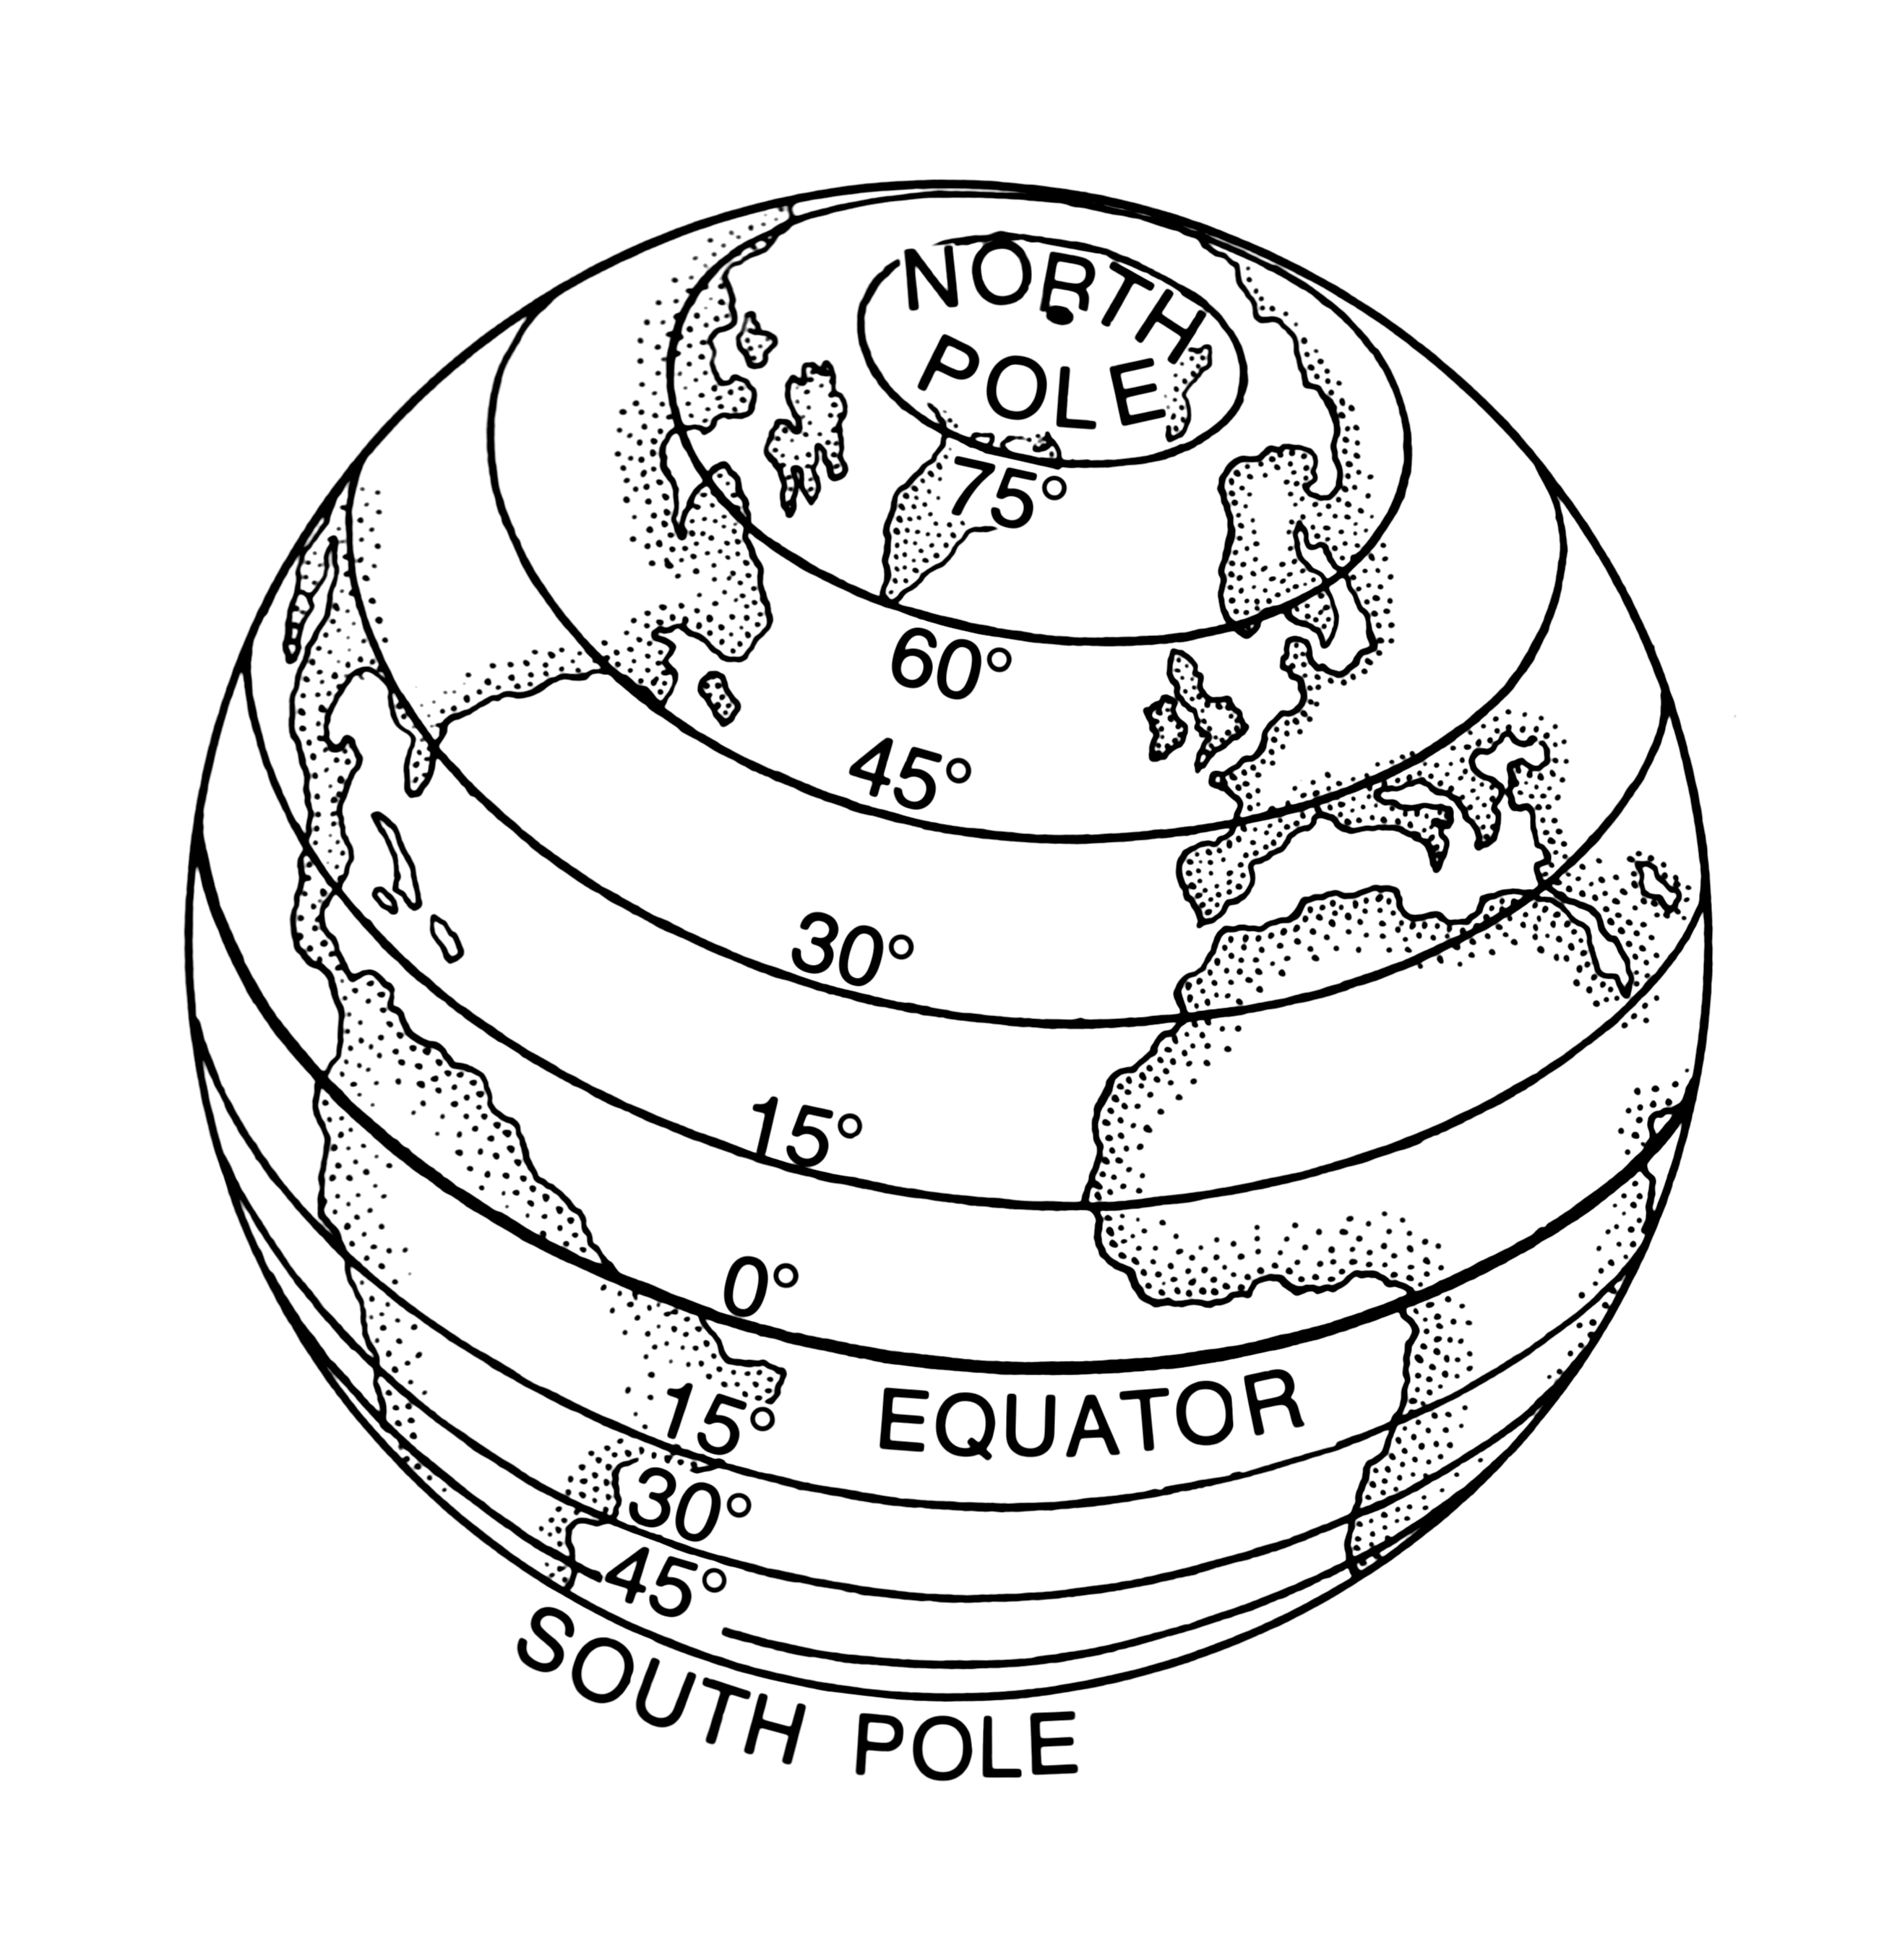
\includegraphics[width=2in]{./RadianMeasureGraphics/Latitude_(PSF).png}

&

\begin{mfpic}[18]{-5}{5}{-4}{4.75}
\axes
\tlabel(4.75,-0.5){\scriptsize $x$}
\tlabel(0.25,4.5){\scriptsize $y$}
\tlabel(3.1,-0.75){\scriptsize $3960$}
\tlabel(0.25,3.1){\scriptsize $3960$}
\tlabel(2.5, 1.75){\scriptsize $Q\left(x,y\right)$}
\tlabel(1.2, 0.15){\scriptsize $41.628^{\circ}$}
\tcaption{}
\xmarks{-3 step 3 until 3}
\ymarks{-3 step 3 until 3}
\drawcolor[gray]{0.7}
\circle{(0,0),3}
\drawcolor{black}
\dotted \polyline{(0, 1.993), (2.242, 1.993)}
\arrow \parafcn{5, 35, 5}{dir(t)}
\tcaption{A point on the Earth at $41.628^{\circ}$N}
\penwd{1.25pt}
 \arrow \reverse \arrow \polyline{(5,0), (0,0), (3.737, 3.321)}
\point[4pt]{(0,0),(2.242, 1.993)}
\end{mfpic}

\end{tabular}

\end{enumerate}

Assuming the Earth is a sphere of radius $3960$ miles, a cross-section through the poles produces a circle of radius $3960$ miles. Viewing the Equator as the $x$-axis, the value we seek is the $x$-coordinate of the point $Q(x,y)$ indicated in the figure above on the right.  Using Theorem \ref{cosinesinecircle}, we get $x = 3960 \cos\left(41.628^{\circ}\right) \approx 2960$.  Hence, the radius of the Earth at North Latitude $41.628^{\circ}$ is approximately $2960$ miles. \qed

\end{ex}
 



Theorem \ref{cosinesinecircle} gives us what we need to `circle back' to the question posed at the the beginning of the section:  how to describe the position of an object traveling in a circular path of radius $r$ with constant angular velocity $\omega$.  Suppose that at time $t$, the object has swept out an angle measuring $\theta$ radians.  If we assume that the object is at the point $(r,0)$ when $t=0$, the angle $\theta$ is in standard position.  By definition, $\omega = \frac{\theta}{t}$ which we rewrite as  $\theta = \omega t$.  According to Theorem \ref{cosinesinecircle}, the location of the object $Q(x,y)$ on the circle is found using the equations  $x = r \cos(\theta) = r \cos(\omega t)$ and $y = r \sin(\theta) = r \sin(\omega t)$.  Hence, at time $t$, the object is at the point $(r \cos(\omega t), r \sin(\omega t))$, as seen in the diagram below.

\begin{center}

\hspace{.55in} \begin{mfpic}[15]{-5}{5}{-5}{5}
\axes
\tlabel(4.75,-0.5){\scriptsize $x$}
\tlabel(0.25,4.75){\scriptsize $y$}
\tlabel(2.1,-0.75){\scriptsize $1$}
\tlabel(0.25,2.1){\scriptsize $1$}
\tlabel(4.1,-0.75){\scriptsize $r$}
\tlabel(0.25,4.1){\scriptsize $r$}
\tlabel(2.35, 3.5){\small $Q\left(x,y\right) = (r \cos(\omega t), r \sin(\omega t))$}
\xmarks{-4 step 2 until 4}
\ymarks{-4 step 2 until 4}
\drawcolor[gray]{0.7}
\circle{(0,0),4}
\drawcolor{black}
\arrow \reverse \arrow \polyline{(5,0),(0,0), (2.5, 4.3301)}
\arrow \parafcn{5, 55, 5}{dir(t)}
\tlabel[cc](1.95, .5){\small $\theta = \omega t$}
\point[4pt]{(0,0),  (2, 3.4641)}
\penwd{1.5pt}
\arrow \parafcn{0, 60, 5}{4*dir(t)}
\end{mfpic} 

\hspace{-.7in} Equations for Circular Motion

\end{center}



 We have just argued the following.


\smallskip

\colorbox{ResultColor}{\bbm
\begin{eqn} \label{equationsforcircularmotion} Suppose an object is traveling in a circular path of radius $r$ centered at the origin with constant angular velocity $\omega$.  If $t=0$ corresponds to the point $(r,0)$, then the $x$ and $y$ coordinates of the object are functions of $t$ and are given by $x =  r \cos(\omega t)$ and $y = r \sin(\omega t)$.  Here, $\omega > 0$ indicates a counter-clockwise direction and $\omega < 0$ indicates a clockwise direction.

\end{eqn}
\ebm}
\smallskip

\begin{ex}  Suppose we are in the situation of Example \ref{EarthRotationEx}.  Find the equations of motion of Lakeland Community College as the earth rotates.
\label{Lakelandrotates}

\smallskip

{\bf Solution.}  From Example \ref{EarthRotationEx}, we take $r = 2960$ miles and and $\omega = \frac{\pi}{12 \, \text{hours}}$.  Hence, the equations of motion are $x =  r \cos(\omega t) = 2960 \cos\left(\frac{\pi}{12} t\right)$ and  $y =  r \sin(\omega t) = 2960 \sin\left(\frac{\pi}{12} t\right)$, where $x$ and $y$ are measured in miles and $t$ is measured in hours.\footnote{We will revisit this concept of associating points with times in Section \ref{ParametricEquations}.} \qed

\end{ex}




\newpage

\subsection{Exercises}


In Exercises \ref{valuefirst} - \ref{valuelast}, find the exact value of the cosine and sine of the given angle.

\begin{multicols}{4}

\begin{enumerate}

\item $\theta = 0$ \vphantom{$\dfrac{\pi}{4}$} \label{valuefirst}
\item $\theta = \dfrac{\pi}{4}$
\item $\theta = \dfrac{\pi}{3}$
\item $\theta = \dfrac{\pi}{2}$

\setcounter{HW}{\value{enumi}}

\end{enumerate}

\end{multicols}

\begin{multicols}{4}

\begin{enumerate}

\setcounter{enumi}{\value{HW}}

\item $\theta = \dfrac{2\pi}{3}$
\item $\theta = \dfrac{3\pi}{4}$
\item $\theta = \pi$ \vphantom{$\dfrac{7\pi}{4}$}
\item $\theta = \dfrac{7\pi}{6}$

\setcounter{HW}{\value{enumi}}

\end{enumerate}

\end{multicols}

\begin{multicols}{4}

\begin{enumerate}

\setcounter{enumi}{\value{HW}}

\item $\theta = \dfrac{5\pi}{4}$
\item $\theta = \dfrac{4\pi}{3}$
\item $\theta = \dfrac{3\pi}{2}$
\item $\theta = \dfrac{5\pi}{3}$

\setcounter{HW}{\value{enumi}}

\end{enumerate}

\end{multicols}

\begin{multicols}{4}

\begin{enumerate}

\setcounter{enumi}{\value{HW}}

\item $\theta = \dfrac{7\pi}{4}$
\item $\theta = \dfrac{23\pi}{6}$
\item $\theta = -\dfrac{13\pi}{2}$
\item $\theta = -\dfrac{43\pi}{6}$

\setcounter{HW}{\value{enumi}}

\end{enumerate}

\end{multicols}

\begin{multicols}{4}

\begin{enumerate}

\setcounter{enumi}{\value{HW}}

\item $\theta = -\dfrac{3\pi}{4}$
\item $\theta = -\dfrac{\pi}{6}$ \vphantom{$\dfrac{7\pi}{4}$}
\item $\theta = \dfrac{10\pi}{3}$
\item $\theta = 117\pi$ \vphantom{$\dfrac{7\pi}{4}$} \label{valuelast}

\setcounter{HW}{\value{enumi}}

\end{enumerate}

\end{multicols}

In Exercises \ref{solveforanglefirst} - \ref{solveforanglelast}, find all of the angles which satisfy the given equation.

\begin{multicols}{3}

\begin{enumerate}

\setcounter{enumi}{\value{HW}}

\item $\sin(\theta) = \dfrac{1}{2}$ \vphantom{$\dfrac{2}{2}$} \label{solveforanglefirst}
\item $\cos(\theta) = -\dfrac{\sqrt{3}}{2}$
\item $\sin(\theta) = 0$ \vphantom{$\dfrac{2}{2}$}

\setcounter{HW}{\value{enumi}}

\end{enumerate}

\end{multicols}

\begin{multicols}{3}

\begin{enumerate}

\setcounter{enumi}{\value{HW}}

\item $\cos(\theta) = \dfrac{\sqrt{2}}{2}$
\item $\sin(\theta) = \dfrac{\sqrt{3}}{2}$
\item $\cos(\theta) = -1$ \vphantom{$\dfrac{\sqrt{2}}{2}$}

\setcounter{HW}{\value{enumi}}

\end{enumerate}

\end{multicols}

\begin{multicols}{3}

\begin{enumerate}

\setcounter{enumi}{\value{HW}}

\item  $\sin(\theta) = -1$ \vphantom{$\dfrac{\sqrt{2}}{2}$}
\item  $\cos(\theta) = \dfrac{\sqrt{3}}{2}$
\item  $\cos(\theta) = -1.001$ \vphantom{$\dfrac{\sqrt{2}}{2}$} \label{solveforanglelast}

\setcounter{HW}{\value{enumi}}

\end{enumerate}

\end{multicols}

In Exercises \ref{solvefortfirst} - \ref{solvefortlast}, solve the equation for $t$.  (See the remarks on page \ref{cosinesineequationsrealnumbers}.)

\begin{multicols}{3}

\begin{enumerate}

\setcounter{enumi}{\value{HW}}

\item $\cos(t) = 0$ \vphantom{$\dfrac{\sqrt{2}}{2}$} \label{solvefortfirst}
\item $\sin(t) = -\dfrac{\sqrt{2}}{2}$
\item $\cos(t) = 3$ \vphantom{$\dfrac{\sqrt{2}}{2}$}

\setcounter{HW}{\value{enumi}}

\end{enumerate}

\end{multicols}

\begin{multicols}{3}

\begin{enumerate}

\setcounter{enumi}{\value{HW}}

\item $\sin(t) = -\dfrac{1}{2}$
\item $\cos(t) = \dfrac{1}{2}$
\item $\sin(t) = -2$ \vphantom{$\dfrac{1}{2}$}

\setcounter{HW}{\value{enumi}}

\end{enumerate}

\end{multicols}

\begin{multicols}{3}

\begin{enumerate}

\setcounter{enumi}{\value{HW}}

\item $\cos(t) = 1$ \vphantom{$\dfrac{\sqrt{2}}{2}$}
\item $\sin(t) = 1$ \vphantom{$\dfrac{\sqrt{2}}{2}$}
\item $\cos(t) = -\dfrac{\sqrt{2}}{2}$ \label{solvefortlast}

\setcounter{HW}{\value{enumi}}

\end{enumerate}

\end{multicols}

In Exercises \ref{pointsfirst} - \ref{pointslast}, let $\theta$ be the angle in standard position whose terminal side contains the given point then compute $\cos(\theta)$ and $\sin(\theta)$.

\begin{multicols}{4}

\begin{enumerate}

\setcounter{enumi}{\value{HW}}

\item $P(-7, 24)$ \label{pointsfirst} 
\item $Q(3, 4)$
\item $R(5, -9)$
\item $T(-2, -11)$ \label{pointslast}

\setcounter{HW}{\value{enumi}}

\end{enumerate}

\end{multicols}

\newpage

In Exercises \ref{findthevaluefirst} - \ref{findthevaluelast}, use the results developed throughout the section to find the requested value.

\begin{enumerate}

\setcounter{enumi}{\value{HW}}

\item If $\sin(\theta) = -\dfrac{7}{25}$ with $\theta$ in Quadrant IV, what is $\cos(\theta)$? \label{findthevaluefirst}
\item If $\cos(\theta) = \dfrac{4}{9}$ with $\theta$ in Quadrant I, what is $\sin(\theta)$?
\item If $\sin(\theta) = \dfrac{5}{13}$ with $\theta$ in Quadrant II, what is $\cos(\theta)$?
\item If $\cos(\theta) = -\dfrac{2}{11}$ with $\theta$ in Quadrant III, what is $\sin(\theta)$?
\item If $\sin(\theta) = -\dfrac{2}{3}$ with $\theta$ in Quadrant III, what is $\cos(\theta)$?
\item If $\cos(\theta) = \dfrac{28}{53}$ with $\theta$ in Quadrant IV, what is $\sin(\theta)$?
\item  If $\sin(\theta) = \dfrac{2\sqrt{5}}{5}$ and $\dfrac{\pi}{2} < \theta < \pi$, what is $\cos(\theta)$?
\item  If $\cos(\theta) = \dfrac{\sqrt{10}}{10}$ and $2\pi < \theta < \dfrac{5\pi}{2}$, what is $\sin(\theta)$?
\item  If $\sin(\theta) = -0.42$ and $\pi < \theta < \dfrac{3\pi}{2}$, what is  $\cos(\theta)$?
\item  If $\cos(\theta) = -0.98$ and $\dfrac{\pi}{2} < \theta < \pi$, what is $\sin(\theta)$? \label{findthevaluelast}

\setcounter{HW}{\value{enumi}}

\end{enumerate}

In Exercises \ref{calculatorfirst} - \ref{calculatorlast}, use your calculator to approximate the given value to three decimal places.  Make sure your calculator is in the proper angle measurement mode!

\begin{multicols}{3}

\begin{enumerate}

\setcounter{enumi}{\value{HW}}

\item $\sin(78.95^{\circ})$ \label{calculatorfirst}
\item $\cos(-2.01)$
\item $\sin(392.994)$

\setcounter{HW}{\value{enumi}}

\end{enumerate}

\end{multicols}

\begin{multicols}{3}

\begin{enumerate}

\setcounter{enumi}{\value{HW}}

\item $\cos(207^{\circ})$
\item $\sin\left( \pi^{\circ} \right)$
\item $\cos(e)$ \label{calculatorlast} 

\setcounter{HW}{\value{enumi}}

\end{enumerate}

\end{multicols}

In Exercises \ref{decomposebasicsinecosinefirst} - \ref{decomposebasicsinecosinelast}, write the given function as a nontrivial decomposition of functions as directed.

\begin{enumerate}
\setcounter{enumi}{\value{HW}}

\item  For $f(t) = 3t + \sin(2t)$, find functions $g$ and $h$ so that $f=g+h$. \label{decomposebasicsinecosinefirst}
\item  For $f(\theta) = 3\cos(\theta) - \sin(4\theta)$, find functions $g$ and $h$ so that $f=g-h$. 
\item  For $f(t) = e^{-0.1t} \sin(3t)$, find functions $g$ and $h$ so that $f=gh$.
\item  For $r(t) = \dfrac{\sin(t)}{t}$, find functions $f$ and $g$ so $r = \dfrac{f}{g}$.
\item  For $r(\theta) =\sqrt{3 \cos(\theta)}$, find functions $f$ and $g$ so $r = g \circ f$. \label{decomposebasicsinecosinelast}

\setcounter{HW}{\value{enumi}}
\end{enumerate}

\begin{enumerate}
\setcounter{enumi}{\value{HW}}

\item \label{sinearcexercise}For each function $S(t)$ listed below, compute the average rate of change over the indicated interval.\footnote{See Definition \ref{arc} in Section \ref{AverageRateofChange} for a review of this concept, as needed.}  What trends do you notice? Be sure your calculator is in radian mode!

\[ \begin{array}{|r||c|c|c|}  \hline

 S(t) &  [-0.1, 0.1] & [-0.01, 0.01] &[-0.001, 0.001] \\ \hline
 \sin(t)     &&&  \\  \hline
 \sin(2t)   &&&  \\ \hline
 \sin(3t)   &&&   \\  \hline
\sin(4t)   &&&   \\  \hline

\end{array} \]

\setcounter{HW}{\value{enumi}}
\end{enumerate}

In Exercises \ref{motionfirst} - \ref{motionlast}, find the equations of motion for the given scenario.  Assume that the center of the motion is the origin, the motion is counter-clockwise and that $t = 0$ corresponds to a position along the positive $x$-axis.  (See Equation \ref{equationsforcircularmotion} and Example \ref{EarthRotationEx}.)

\begin{enumerate}

\setcounter{enumi}{\value{HW}}

\item  \label{motionfirst} A point on the edge of the spinning yo-yo in Exercise \ref{spinningyoyo} from Section \ref{RadianMeasure}. 

Recall: The diameter of the yo-yo is 2.25 inches and it spins at 4500 revolutions per minute.

\item  The yo-yo in exercise \ref{yoyotrick} from Section \ref{RadianMeasure}.

Recall: The radius of the circle is 28 inches and it completes one revolution in 3 seconds.

\item A point on the edge of the hard drive in Exercise \ref{harddrive} from Section \ref{RadianMeasure}.

Recall:  The diameter of the hard disk is 2.5 inches and it spins at 7200 revolutions per minute.

\item  \label{motionlast} A passenger on the Big Wheel in Exercise \ref{giantwheelmotion} from Section \ref{RadianMeasure}.

Recall: The diameter is 128 feet and completes 2 revolutions in 2 minutes, 7 seconds.

\setcounter{HW}{\value{enumi}}

\end{enumerate}

\begin{enumerate}

\setcounter{enumi}{\value{HW}}

\item Consider the numbers:  $0$, $1$, $2$, $3$, $4$.  Take the square root of each of these numbers, then divide each by $2$. The resulting numbers should look hauntingly familiar. (See the values in the table on \pageref{CosineSineFacts}.) 


\item  On page \pageref{cosinesineequationsrealnumbers}, we see that the sine and cosine functions of \textit{angles} can be considered functions of \textit{real numbers}.  With help from your classmates, discuss the domains and ranges of  $f(t) = \sin(t)$ and $g(t) = \cos(t)$.  Write your answers using interval notation.


\item  \label{circleofradiusrsinecosinetrans}  Another way to establish  Theorem \ref{cosinesinecircle} is to use transformations. Re-read the discussion following  Theorem \ref{standardcirclealternate} in Chapter \ref{TheConicSections}  and transform  the Unit Circle, $x^2+y^2 = 1$, to $x^2 + y^2 = r^2$ using horizontal and vertical stretches.  Show if the coordinates on the Unit Circle are $(\cos(\theta), \sin(\theta))$, then the corresponding coordinates on $x^2+y^2 = r^2$ are $(r \cos(\theta), r \sin(\theta))$.

\item  In the scenario of Equation \ref{equationsforcircularmotion}, we assumed that at $t=0$, the object was at the point $(r,0)$.  If this is not the case,  we can adjust the equations of motion by introducing a `time delay.'   If $t_{0} > 0$ is the first time the object passes through the point $(r,0)$, show, with the help of your classmates, the equations of motion are $x = r \cos(\omega (t - t_{0}))$ and $y = r \sin(\omega (t-t_{0}))$.


\end{enumerate}

\newpage

\subsection{Answers}

\begin{multicols}{2}

\begin{enumerate}

\item $\cos(0) = 1$, $\; \sin(0) = 0$ \vphantom{$\dfrac{\sqrt{2}}{2}$}

\item $\cos \left(\dfrac{\pi}{4} \right) = \dfrac{\sqrt{2}}{2}$, $\; \sin \left(\dfrac{\pi}{4} \right) = \dfrac{\sqrt{2}}{2}$

\setcounter{HW}{\value{enumi}}

\end{enumerate}

\end{multicols}

\begin{multicols}{2}

\begin{enumerate}

\setcounter{enumi}{\value{HW}}

\item $\cos \left(\dfrac{\pi}{3}\right) = \dfrac{1}{2}$, $\; \sin \left(\dfrac{\pi}{3}\right) = \dfrac{\sqrt{3}}{2}$

\item $\cos \left(\dfrac{\pi}{2}\right) = 0$, $\; \sin \left(\dfrac{\pi}{2}\right) = 1$ \vphantom{$\dfrac{\sqrt{2}}{2}$}

\setcounter{HW}{\value{enumi}}

\end{enumerate}

\end{multicols}

\begin{multicols}{2}

\begin{enumerate}

\setcounter{enumi}{\value{HW}}

\item $\cos\left(\dfrac{2\pi}{3}\right) = -\dfrac{1}{2}$, $\; \sin \left(\dfrac{2\pi}{3}\right) = \dfrac{\sqrt{3}}{2}$

\item $\cos \left(\dfrac{3\pi}{4} \right) = -\dfrac{\sqrt{2}}{2}$, $\; \sin \left(\dfrac{3\pi}{4} \right) = \dfrac{\sqrt{2}}{2}$

\setcounter{HW}{\value{enumi}}

\end{enumerate}

\end{multicols}

\begin{multicols}{2}

\begin{enumerate}

\setcounter{enumi}{\value{HW}}

\item $\cos(\pi) = -1$, $\; \sin(\pi) = 0$ \vphantom{$\dfrac{\sqrt{3}}{2}$}

\item $\cos\left(\dfrac{7\pi}{6}\right) = -\dfrac{\sqrt{3}}{2}$, $\; \sin\left(\dfrac{7\pi}{6}\right) = -\dfrac{1}{2}$

\setcounter{HW}{\value{enumi}}

\end{enumerate}

\end{multicols}

\begin{multicols}{2}

\begin{enumerate}

\setcounter{enumi}{\value{HW}}

\item $\cos \left(\dfrac{5\pi}{4} \right) = -\dfrac{\sqrt{2}}{2}$, $\; \sin \left(\dfrac{5\pi}{4} \right) = -\dfrac{\sqrt{2}}{2}$

\item $\cos\left(\dfrac{4\pi}{3}\right) = -\dfrac{1}{2}$, $\; \sin \left(\dfrac{4\pi}{3}\right) = -\dfrac{\sqrt{3}}{2}$

\setcounter{HW}{\value{enumi}}

\end{enumerate}

\end{multicols}

\begin{multicols}{2}

\begin{enumerate}

\setcounter{enumi}{\value{HW}}

\item $\cos \left(\dfrac{3\pi}{2}\right) = 0$, $\; \sin \left(\dfrac{3\pi}{2}\right) = -1$

\item $\cos\left(\dfrac{5\pi}{3}\right) = \dfrac{1}{2}$, $\; \sin \left(\dfrac{5\pi}{3}\right) = -\dfrac{\sqrt{3}}{2}$

\setcounter{HW}{\value{enumi}}

\end{enumerate}

\end{multicols}

\begin{multicols}{2}

\begin{enumerate}

\setcounter{enumi}{\value{HW}}

\item $\cos \left(\dfrac{7\pi}{4} \right) = \dfrac{\sqrt{2}}{2}$, $\; \sin \left(\dfrac{7\pi}{4} \right) = -\dfrac{\sqrt{2}}{2}$

\item $\cos\left(\dfrac{23\pi}{6}\right) = \dfrac{\sqrt{3}}{2}$, $\; \sin\left(\dfrac{23\pi}{6}\right) = -\dfrac{1}{2}$

\setcounter{HW}{\value{enumi}}

\end{enumerate}

\end{multicols}

\begin{multicols}{2}

\begin{enumerate}

\setcounter{enumi}{\value{HW}}

\item $\cos \left(-\dfrac{13\pi}{2}\right) = 0$, $\; \sin \left(-\dfrac{13\pi}{2}\right) = -1$ \vphantom{$\dfrac{\sqrt{3}}{2}$}

\item $\cos\left(-\dfrac{43\pi}{6}\right) = -\dfrac{\sqrt{3}}{2}$, $\; \sin\left(-\dfrac{43\pi}{6}\right) = \dfrac{1}{2}$

\setcounter{HW}{\value{enumi}}

\end{enumerate}

\end{multicols}

\begin{multicols}{2}

\begin{enumerate}

\setcounter{enumi}{\value{HW}}

\item $\cos \left(-\dfrac{3\pi}{4} \right) = -\dfrac{\sqrt{2}}{2}$, $\; \sin \left(-\dfrac{3\pi}{4} \right) = -\dfrac{\sqrt{2}}{2}$

\item $\cos\left(-\dfrac{\pi}{6}\right) = \dfrac{\sqrt{3}}{2}$, $\; \sin\left(-\dfrac{\pi}{6}\right) = -\dfrac{1}{2}$

\setcounter{HW}{\value{enumi}}

\end{enumerate}

\end{multicols}

\begin{multicols}{2}

\begin{enumerate}

\setcounter{enumi}{\value{HW}}

\item $\cos\left(\dfrac{10\pi}{3}\right) = -\dfrac{1}{2}$, $\; \sin \left(\dfrac{10\pi}{3}\right) = -\dfrac{\sqrt{3}}{2}$

\item $\cos(117\pi) = -1$, $\; \sin(117\pi) = 0$ \vphantom{$\dfrac{\sqrt{3}}{2}$}

\setcounter{HW}{\value{enumi}}

\end{enumerate}

\end{multicols}

\begin{enumerate}

\setcounter{enumi}{\value{HW}}

\item $\sin(\theta) = \dfrac{1}{2}$ when $\theta = \dfrac{\pi}{6} + 2\pi k$ or $\theta = \dfrac{5\pi}{6} + 2\pi k$ for any integer $k$.
\item $\cos(\theta) = -\dfrac{\sqrt{3}}{2}$ when $\theta = \dfrac{5\pi}{6} + 2\pi k$ or $\theta = \dfrac{7\pi}{6} + 2\pi k$ for any integer $k$.
\item $\sin(\theta) = 0$ when $\theta = \pi k$ for any integer $k$.
\item $\cos(\theta) = \dfrac{\sqrt{2}}{2}$ when $\theta = \dfrac{\pi}{4} + 2\pi k$ or $\theta = \dfrac{7\pi}{4} + 2\pi k$ for any integer $k$.
\item $\sin(\theta) = \dfrac{\sqrt{3}}{2}$ when $\theta = \dfrac{\pi}{3} + 2\pi k$ or $\theta = \dfrac{2\pi}{3} + 2\pi k$ for any integer $k$.
\item $\cos(\theta) = -1$ when $\theta = (2k + 1)\pi$ for any integer $k$.
\item  $\sin(\theta) = -1$ when $\theta = \dfrac{3\pi}{2} + 2\pi k$ for any integer $k$.
\item  $\cos(\theta) = \dfrac{\sqrt{3}}{2}$ when $\theta = \dfrac{\pi}{6} + 2\pi k$ or  $\theta = \dfrac{11\pi}{6} + 2\pi k$ for any integer $k$.
%\item  $\sin(\theta) = \dfrac{\sqrt{2}}{2}$ when $\theta = \dfrac{\pi}{4} + 2\pi k$ or  $\theta = \dfrac{3\pi}{4} + 2\pi k$ for any integer $k$.
\item  $\cos(\theta) = -1.001$ never happens

\setcounter{HW}{\value{enumi}}

\end{enumerate}

\begin{enumerate}

\setcounter{enumi}{\value{HW}}

\item $\cos(t) = 0$ when $t = \dfrac{\pi}{2} + \pi k$ for any integer $k$.
\item $\sin(t) = -\dfrac{\sqrt{2}}{2}$ when $t = \dfrac{5\pi}{4} + 2\pi k$ or $t = \dfrac{7\pi}{4} + 2\pi k$ for any integer $k$.
\item $\cos(t) = 3$ never happens.  
\item $\sin(t) = -\dfrac{1}{2}$ when $t = \dfrac{7\pi}{6} + 2\pi k$ or $t = \dfrac{11\pi}{6} + 2\pi k$ for any integer $k$.
\item $\cos(t) = \dfrac{1}{2}$ when $t = \dfrac{\pi}{3} + 2\pi k$ or $t = \dfrac{5\pi}{3} + 2\pi k$ for any integer $k$.
\item $\sin(t) = -2$ never happens
\item $\cos(t) = 1$ when $t = 2\pi k$ for any integer $k$.
\item $\sin(t) = 1$ when $t = \dfrac{\pi}{2} + 2\pi k$ for any integer $k$.
\item $\cos(t) = -\dfrac{\sqrt{2}}{2}$ when $t = \dfrac{3\pi}{4} + 2\pi k$ or $t = \dfrac{5\pi}{4} + 2\pi k$ for any integer $k$.
%\item  $\sin(t) = -\dfrac{\sqrt{3}}{2}$ when $t = \dfrac{4\pi}{3} + 2\pi k$ or  $t = \dfrac{5\pi}{3} + 2\pi k$ for any integer $k$.

\setcounter{HW}{\value{enumi}}

\end{enumerate}

\begin{enumerate}

\setcounter{enumi}{\value{HW}}

\item $\cos(\theta) = -\dfrac{7}{25}, \; \sin(\theta) = \dfrac{24}{25}$

\item $\cos(\theta) = \dfrac{3}{5}, \; \sin(\theta) = \dfrac{4}{5}$

\item $\cos(\theta) = \dfrac{5\sqrt{106}}{106}, \; \sin(\theta) = -\dfrac{9\sqrt{106}}{106}$

\item $\cos(\theta) = -\dfrac{2\sqrt{5}}{25}, \; \sin(\theta) = -\dfrac{11\sqrt{5}}{25}$

\setcounter{HW}{\value{enumi}}

\end{enumerate}


\begin{enumerate}

\setcounter{enumi}{\value{HW}}

\item If $\sin(\theta) = -\dfrac{7}{25}$ with $\theta$ in Quadrant IV, then $\cos(\theta) = \dfrac{24}{25}$.
\item If $\cos(\theta) = \dfrac{4}{9}$ with $\theta$ in Quadrant I, then $\sin(\theta) = \dfrac{\sqrt{65}}{9}$.
\item If $\sin(\theta) = \dfrac{5}{13}$ with $\theta$ in Quadrant II, then $\cos(\theta) = -\dfrac{12}{13}$.
\item If $\cos(\theta) = -\dfrac{2}{11}$ with $\theta$ in Quadrant III, then $\sin(\theta) = -\dfrac{\sqrt{117}}{11}$.
\item If $\sin(\theta) = -\dfrac{2}{3}$ with $\theta$ in Quadrant III, then $\cos(\theta) = -\dfrac{\sqrt{5}}{3}$.
\item If $\cos(\theta) = \dfrac{28}{53}$ with $\theta$ in Quadrant IV, then $\sin(\theta) = -\dfrac{45}{53}$.
\item  If $\sin(\theta) = \dfrac{2\sqrt{5}}{5}$ and $\dfrac{\pi}{2} < \theta < \pi$, then $\cos(\theta) = -\dfrac{\sqrt{5}}{5}$.
\item  If $\cos(\theta) = \dfrac{\sqrt{10}}{10}$ and $2\pi < \theta < \dfrac{5\pi}{2}$, then $\sin(\theta)  = \dfrac{3 \sqrt{10}}{10}$.
\item  If $\sin(\theta) = -0.42$ and $\pi < \theta < \dfrac{3\pi}{2}$, then $\cos(\theta) = -\sqrt{0.8236} \approx -0.9075$.
\item  If $\cos(\theta) = -0.98$ and $\dfrac{\pi}{2} < \theta < \pi$, then $\sin(\theta) = \sqrt{0.0396} \approx 0.1990$.

\setcounter{HW}{\value{enumi}}

\end{enumerate}


\begin{multicols}{3}

\begin{enumerate}

\setcounter{enumi}{\value{HW}}

\item $\sin(78.95^{\circ}) \approx 0.981$
\item $\cos(-2.01) \approx -0.425$
\item $\sin(392.994) \approx -0.291$

\setcounter{HW}{\value{enumi}}

\end{enumerate}

\end{multicols}

\begin{multicols}{3}

\begin{enumerate}

\setcounter{enumi}{\value{HW}}

\item $\cos(207^{\circ}) \approx -0.891$
\item $\sin\left( \pi^{\circ} \right) \approx 0.055$
\item $\cos(e) \approx -0.912$

\setcounter{HW}{\value{enumi}}

\end{enumerate}
\end{multicols}

\begin{enumerate}
\setcounter{enumi}{\value{HW}}

\item One solution is $g(t) = 3t$ and $h(t) = \sin(2t)$.
\item One solution is $g(\theta) = 3 \cos(\theta)$ and $h(\theta) = \sin(4 \theta)$.
\item One solution is $g(t) =  e^{-0.1t}$ and $h(t) = \sin(3t)$. 
\item One solution is $f(t) = \sin(t)$ and $g(t) = t$.
\item One solution is $f(\theta) = 3 \cos(\theta)$ and $g(\theta) = \sqrt{\theta}$.

\setcounter{HW}{\value{enumi}}
\end{enumerate}

\begin{enumerate}
\setcounter{enumi}{\value{HW}}

\item  As we zoom in towards $0$, the average rate of change of $\sin(k t)$ approaches $k$.

\[ \begin{array}{|r||c|c|c|}  \hline

 S(t) &  [-0.1, 0.1] & [-0.01, 0.01] &[-0.001, 0.001] \\ \hline
 \sin(t)     & \approx 0.9983  &  \approx 1  &  \approx 1 \\  \hline
 \sin(2t)   & \approx 1.9867 & \approx  1.9999 & \approx 2 \\ \hline
 \sin(3t)   & \approx 2.9552 & \approx 2.9995 &  \approx 3  \\  \hline
 \sin(4t)  & \approx 3.8942 & \approx 3.9989 &  \approx 4 \\  \hline

\end{array} \]

\setcounter{HW}{\value{enumi}}
\end{enumerate}


\begin{enumerate}

\setcounter{enumi}{\value{HW}}

\item   $r = 1.125$ inches, $\omega = 9000 \pi \, \frac{\text{radians}}{\text{minute}}$,  $x = 1.125 \cos(9000 \pi \, t)$, $y = 1.125 \sin(9000 \pi \, t)$.  Here $x$ and $y$ are measured in inches and $t$ is measured in minutes.

\item   $r = 28$ inches, $\omega = \frac{2\pi}{3} \, \frac{\text{radians}}{\text{second}}$,  $x = 28 \cos\left(\frac{2\pi}{3} \, t \right)$, $y = 28 \sin\left(\frac{2\pi}{3} \, t \right)$.  Here $x$ and $y$ are measured in inches and $t$ is measured in seconds.

\item $r = 1.25$ inches, $\omega = 14400 \pi \, \frac{\text{radians}}{\text{minute}}$,  $x = 1.25 \cos(14400 \pi \, t)$, $y = 1.25 \sin(14400 \pi \, t)$.  Here $x$ and $y$ are measured in inches and $t$ is measured in minutes.

\item  $r = 64$ feet, $\omega = \frac{4\pi}{127} \, \frac{\text{radians}}{\text{second}}$,  $x = 64 \cos\left(\frac{4\pi}{127} \, t \right)$, $y = 64 \sin\left(\frac{4\pi}{127} \, t \right)$.  Here $x$ and $y$ are measured in feet and $t$ is measured in seconds

\end{enumerate}


\closegraphsfile

\newpage

\section{Graphs of Sine and Cosine}

\mfpicnumber{1}

\opengraphsfile{GraphsofSineandCosine}

\setcounter{footnote}{0}

\label{GraphsofSineandCosine}

On page \pageref{cosinesineequationsrealnumbers}, we discussed how to interpret the sine and cosine of real numbers.  To review, we identify a real number  $t$ with an oriented angle $\theta$ measuring $t$ radians\footnote{which, you'll recall  essentially `wraps the real number line around the Unit Circle}   and define $\sin(t) = \sin(\theta)$ and $\cos(t) = \cos(\theta)$.  Since every real number can be identified with one and only one angle $\theta$ this way, the domains of the functions $f(t) = \sin(t)$ and $g(t) = \cos(t)$ are all real numbers, $(-\infty, \infty)$.

\smallskip

When it comes to range, recall that the sine and cosine of angles are coordinates of points on the Unit Circle and hence, each  fall between $-1$ and $1$ inclusive.  Since the real number line,\footnote{in particular the interval $[0, 2\pi)$} when wrapped around the Unit Circle completely covers the circle, we can be assured that every point on the Unit Circle corresponds to at least one real number.  Putting these two facts together, we conclude the range of $f(t) = \sin(t)$ and $g(t) = \cos(t)$ are both $[-1,1]$.  We summarize these two important facts below.


\smallskip

\colorbox{ResultColor}{\bbm

\begin{thm} \label{cosinesinefunctiondomainrange}  \textbf{Domain and Range of the Cosine and Sine Functions:} 

\vspace{.2in}

\begin{tabular}{ll}

\hspace{.3in} $\bullet \, $ The function $f(t) = \sin(t)$ & \hspace{.8in} $\bullet \, $ The function $g(t) = \cos(t)$ \\ [4pt]
\hspace{.5in} -- has domain $(-\infty, \infty)$ & \hspace{1in} -- has domain $(-\infty, \infty)$ \\ [4pt]
\hspace{.5in} -- has range $[-1,1]$ & \hspace{1in} -- has range $[-1,1]$ \\ [4pt]

\end{tabular}

\end{thm}

\ebm}

\smallskip

Our aim in this section is to become familiar with the graphs of $f(t) = \sin(t)$ and $g(t) = \cos(t)$.  To that end, we begin by making a table and plotting points.  We'll start by graphing $f(t) = \sin(t)$ by making a table of values and plotting the corresponding points.  We'll keep the independent variable `$t$' for now and use the default `$y$' as our dependent variable.\footnote{Keep in mind that we're using `$y$' here to denote the \textit{output} from the sine function.  It is a coincidence that the $y$-values on the graph of $y=\sin(t)$ correspond to the $y$-values on the Unit Circle.}  Note in the graph below, on the right,  the scale of the horizontal and vertical axis is far from 1:1.  (We will present a more accurately scaled graph shortly.)


\hspace{.5in} \begin{tabular}{m{2.7in}m{3in}}
\setlength{\extrarowheight}{2pt}
\[ \begin{array}{|r||r|r|}  

\hline

 t & \sin(t) & (t,\sin(t)) \\ \hline
0  & 0 & (0, 0) \\ [2pt]   \hline
\frac{\pi}{4}  & \frac{\sqrt{2}}{2} & \left(\frac{\pi}{4}, \frac{\sqrt{2}}{2}\right) \\ [2pt] \hline 
\frac{\pi}{2}  & 1 & \left(\frac{\pi}{2}, 1\right) \\ [2pt] \hline 
\frac{3\pi}{4}  & \frac{\sqrt{2}}{2} & \left(\frac{3\pi}{4}, \frac{\sqrt{2}}{2}\right) \\ [2pt] \hline 
\pi & 0 & (\pi, 0) \\ [2pt] \hline 
\frac{5\pi}{4}  & -\frac{\sqrt{2}}{2} & \left(\frac{5\pi}{4}, -\frac{\sqrt{2}}{2}\right) \\ [2pt] \hline 
\frac{3\pi}{2}  & -1 & \left(\frac{3\pi}{2}, -1 \right) \\ [2pt] \hline 
\frac{7\pi}{4}  & -\frac{\sqrt{2}}{2} & \left(\frac{7\pi}{4}, -\frac{\sqrt{2}}{2}\right) \\ [2pt] \hline 
2\pi  & 0 & (2\pi, 0) \\  [2pt] \hline
\end{array} \] \setlength{\extrarowheight}{0pt} &

\begin{mfpic}[25][50]{-1}{7}{-1.5}{1.5}
\point[4pt]{(0,0), (0.7854,0.7071), (1.5708,1), (2.3562,0.7071), (3.1416, 0), (3.9270,-0.7071), (4.7124,-1), (5.4978,-0.7071), (6.2832,0)}
\axes
\tlabel[cc](7,-0.15){\scriptsize $t$}
\tlabel[cc](0.25,1.5){\scriptsize $y$}
\tcaption{Graphing $y = \sin(t)$.}
\xmarks{0.7854, 1.5708, 2.3562, 3.1416, 3.9270, 4.7124,5.4978,6.2832 }
\ymarks{-1,1}
\tlpointsep{4pt}
\scriptsize
\axislabels {x}{{$\frac{\pi}{4}$} 0.7854, {$\frac{\pi}{2}$} 1.5708, {$\frac{3\pi}{4}$} 2.3562, {$\pi$} 3.1416, {$\frac{5\pi}{4}$} 3.9270, {$\frac{3\pi}{2}$} 4.7124, {$\frac{7\pi}{4}$} 5.4978, {$2\pi$} 6.2832}
\normalsize
\axislabels {y}{{\scriptsize $-1$} -1, {\scriptsize $1$} 1}
\penwd{1.1pt}
\function{0, 6.2832, 0.1}{sin(x)}
\end{mfpic} \\

\end{tabular}

If we plot additional points, we soon find that the graph repeats itself.   This shouldn't come as too much of a surprise considering Theorem \ref{coterminalsamcosinesinethm}.  In fact, in light of that theorem, we expect the function to repeat itself every $2\pi$ units.  Below is a more accurately scaled graph highlighting the portion we had already graphed above.  The graph is often described as having a `wavelike' nature and is sometimes called a \index{wave ! sine}\index{sine wave} \textbf{sine wave} or, more technically, a \index{sinusoid}\textbf{sinusoid}.

\smallskip

\begin{center}

\begin{mfpic}[15]{-13}{13}{-1.5}{1.5}
\axes
\point[4pt]{(0,0), (6.2832,0)}
\tlabel[cc](13,-0.5){\scriptsize $t$}
%\tlabel[cc](0.5,1.5){\scriptsize $y$}
\tlabel[cc](0.5,1.25){\scriptsize $1$}
\tlabel[cc](0.5,-1){\scriptsize $-1$}
\tcaption{A more accurately scaled graph of $f(t) = \sin(t)$.}
\ymarks{-1,1}
\arrow \reverse \arrow \function{-12, 12, 0.1}{sin(x)}
\penwd{1.5pt}
\function{0, 6.2832, 0.1}{sin(x)}
\end{mfpic}

\end{center}

Note that by copying  the highlighted portion of the graph and pasting it end-to-end, we obtain the entire graph of $f(t) = \sin(t)$.  We give this `repeating' property a name.

\smallskip

\colorbox{ResultColor}{\bbm

\begin{defn} \label{periodic} \textbf{Periodic Functions:} A function $f$ is said to be \textbf{periodic}\index{function ! periodic}\index{periodic function}  if there is a real number $c$ so that $f(t+c) = f(t)$ for all real numbers $t$ in the domain of $f$.  The smallest positive number $p$ for which $f(t+p) = f(t)$ for all real numbers $t$ in the domain of $f$, if it exists, is called the \textbf{period} of $f$. \index{period ! of a function}

\end{defn}

\ebm}

\medskip

We have already seen a family of periodic functions in Section \ref{ConstantandLinearFunctions}:  the constant functions.  However, despite being periodic a constant function has no period.  (We'll leave that odd gem as an exercise for you.)  

\smallskip

Returning to $f(t) = \sin(t)$, we see that by Definition \ref{periodic}, $f$ is periodic since $\sin(t + 2\pi) = \sin(t)$.  To determine the period of $f$, we need to find the smallest real number $p$ so that $f(t+p) = f(t)$ for all real numbers $t$ or, said differently, the smallest positive real number $p$ such that $\sin(t+p) = \sin(t)$  for all real numbers $t$.  

\smallskip

We know that $\sin(t + 2\pi) = \sin(t)$ for all real numbers $t$ but the question remains if any smaller real number will do the trick.  Suppose $p>0$ and $\sin(t + p) = \sin(t)$ for all real numbers $t$.  Then, in particular, $\sin(0+p) = \sin(0)=0$ so that $\sin(p) = 0$.  From this we know $p$ is a multiple of $\pi$.  Since $\sin\left(\frac{\pi}{2} \right)  \neq \sin\left(\frac{\pi}{2} + \pi \right) $, we know $p \neq \pi$.  Hence, $p  = 2\pi$ so the period of $f(t) = \sin(t)$ is $2\pi$. 

\smallskip

Having period $2\pi$ essentially means that we can completely understand everything about the function  $f(t) =  \sin(t)$ by studying \textit{one} interval of length $2\pi$, say $[0,2\pi]$.\footnote{Technically, we should study the interval $[0,2\pi)$,\footnotemark since whatever happens at $t=2\pi$ is the same as what happens at $t=0$.  As we will see shortly, $t=2\pi$ gives us an extra `check' when we go to graph these functions.} \footnotetext{In some advanced texts, the interval of choice is $[-\pi, \pi)$.}  For this reason, when graphing sine (and cosine) functions, we typically restrict our attention to graphing these functions over the course of one period to produce one \index{cycle ! of $\sin(t)$ and $\cos(t)$}\textbf{cycle} of the graph. 
 
\smallskip


Not surprisingly, the graph of $g(t) = \cos(t)$ exhibits similar behavior as $f(t) = \sin(t)$ as seen below.\footnote{Here note that the dependent variable `$y$' represents the outputs from  $g(t) = \cos(t)$ which are $x$-coordinates on the Unit CIrcle.}  

\hspace{.5in} \begin{tabular}{m{2.7in}m{3in}}
\setlength{\extrarowheight}{2pt}
\[ \begin{array}{|r||r|r|}  

\hline

 t & \cos(t) & (t,\cos(t)) \\ \hline
0  & 1 & (0, 1) \\ [2pt]   \hline
\frac{\pi}{4}  & \frac{\sqrt{2}}{2} & \left(\frac{\pi}{4}, \frac{\sqrt{2}}{2}\right) \\ [2pt] \hline 
\frac{\pi}{2}  & 0 & \left(\frac{\pi}{2}, 0\right) \\ [2pt] \hline 
\frac{3\pi}{4}  & -\frac{\sqrt{2}}{2} & \left(\frac{3\pi}{4}, -\frac{\sqrt{2}}{2}\right) \\ [2pt] \hline 
\pi & -1 & (\pi, -1) \\ [2pt] \hline 
\frac{5\pi}{4}  & -\frac{\sqrt{2}}{2} & \left(\frac{5\pi}{4}, -\frac{\sqrt{2}}{2}\right) \\ [2pt] \hline 
\frac{3\pi}{2}  & 0 & \left(\frac{3\pi}{2}, 0 \right) \\ [2pt] \hline 
\frac{7\pi}{4}  & \frac{\sqrt{2}}{2} & \left(\frac{7\pi}{4}, \frac{\sqrt{2}}{2}\right) \\ [2pt] \hline 
2\pi  & 1 & (2\pi, 1) \\  [2pt] \hline
\end{array} \] \setlength{\extrarowheight}{0pt} &

\begin{mfpic}[25][50]{-1}{7}{-1.5}{1.5}
\point[4pt]{(0,1), (0.7854,0.7071), (1.5708,0), (2.3562,-0.7071), (3.1416, -1), (3.9270,-0.7071), (4.7124,0), (5.4978,0.7071), (6.2832,1)}
\axes
\tlabel[cc](7,-0.15){\scriptsize $t$}
\tlabel[cc](0.25,1.5){\scriptsize $y$}
\tcaption{Graphing $y = \cos(t)$.}
\xmarks{0.7854, 1.5708, 2.3562, 3.1416, 3.9270, 4.7124,5.4978,6.2832 }
\ymarks{-1,1}
\tlpointsep{4pt}
\scriptsize
\axislabels {x}{{$\frac{\pi}{4}$} 0.7854, {$\frac{\pi}{2}$} 1.5708, {$\frac{3\pi}{4}$} 2.3562, {$\pi$} 3.1416, {$\frac{5\pi}{4}$} 3.9270, {$\frac{3\pi}{2}$} 4.7124, {$\frac{7\pi}{4}$} 5.4978, {$2\pi$} 6.2832}
\normalsize
\axislabels {y}{{\scriptsize $-1$} -1, {\scriptsize $1$} 1}
\penwd{1.25pt}
\function{0, 6.2832, 0.1}{cos(x)}
\end{mfpic} \\

\end{tabular}

\smallskip

Like $f(t)=\sin(t)$, $g(t) = \cos(t)$ is a wavelike curve with period $2\pi$.   Moreover, the graphs of the sine and cosine functions have the same shape -  differing only in what appears to be a horizontal shift.  As we'll prove in Section \ref{MoreTrigonometricIdentities}, $\sin\left(t + \frac{\pi}{2}\right) = \cos(t)$, which means we can obtain the graph of $y=\cos(t)$ by shifting the graph of $y=\sin(t)$ to the left $\frac{\pi}{2}$ units.\footnote{Hence, we can obtain the graph of $y = \sin(t)$ by shifting the graph of $y = \cos(t)$ to the \textit{right} $\frac{\pi}{2}$ units: $\cos\left(t - \frac{\pi}{2} \right) = \sin(t)$.}


\smallskip

\begin{center}

\begin{mfpic}[15]{-13}{13}{-1.5}{1.5}
\axes
\point[4pt]{(0,1), (6.2832,1)}
\tlabel[cc](13,-0.5){\scriptsize $t$}
%\tlabel[cc](0.5,1.5){\scriptsize $y$}
\tcaption{The graph of $g(t) = \cos(t)$.}
\ymarks{-1,1}
\tlabel[cc](0.5,1.25){\scriptsize $1$}
\tlabel[cc](0.5,-1){\scriptsize $-1$}
\arrow \reverse \arrow \function{-12.5664, 12.5664, 0.1}{cos(x)}
\penwd{1.5pt}
\function{0, 6.2832, 0.1}{cos(x)}
\end{mfpic}

\end{center}

\smallskip

While arguably the most important property shared by  $f(t) = \sin(t)$ and $g(t) = \cos(t)$ is their periodic `wavelike' nature,\footnote{this is the reason they are so useful in the Sciences and Engineering} their graphs suggest these functions are both continuous and smooth.  Recall from Section \ref{GraphsofPolynomials} that, like polynomial functions, the graphs of the sine and cosine functions have no jumps, gaps, holes in the graph,  vertical asymptotes, corners or cusps.  

\smallskip

Moreover,  the graphs of both $f(t) = \sin(t)$ and $g(t) = \cos(t)$ meander and  never `settle down' as $t \rightarrow \pm \infty$ to any one real number.  So even though these functions are `trapped' (or \index{bounded}\textbf{bounded}) between $-1$ and $1$, neither graph has any horizontal asymototes.

\smallskip

Lastly, the graphs of  $f(t) = \sin(t)$ and $g(t) = \cos(t)$ suggest each enjoy one of the symmetries introduced in Section \ref{GraphsofPolynomials}.  The graph of $y = \sin(t)$ appears to be symmetric about the origin while the graph of $y = \cos(t)$ appears to be symmetric about the $y$-axis.  Indeed, as we'll prove in Section \ref{MoreTrigonometricIdentities}, $f(t) = \sin(t)$ is, in fact, an odd function: \footnote{The reader may wish to review Definitions  \ref{evenfunctiondefn} and  \ref{oddfunctiondefn} as needed.}  that is, $\sin(-t) = -\sin(t)$ and  $g(t) = \cos(t)$ is an even function, so $\cos(-t) = \cos(t)$.  

\smallskip

 We summarize all of these properties in the following result.

\smallskip

\colorbox{ResultColor}{\bbm

\begin{thm} \label{cosinesinefunctionprops}  \textbf{Properties of the Cosine and Sine Functions} \index{cosine ! properties of} \index{sine ! properties of}

\vspace{.2in}

\begin{tabular}{ll}

\hspace{.3in} $\bullet \, $ The function $f(t) = \sin(t)$ & \hspace{.8in} $\bullet \, $ The function $g(t) = \cos(t)$ \\
  & \\

\hspace{.5in} -- has domain $(-\infty, \infty)$ & \hspace{1in} -- has domain $(-\infty, \infty)$ \\ [4pt]
\hspace{.5in} -- has range $[-1,1]$ & \hspace{1in} -- has range $[-1,1]$ \\ [4pt]
\hspace{.5in} -- is continuous and smooth & \hspace{1in} -- is continuous and smooth \\ [4pt]
\hspace{.5in} -- is odd & \hspace{1in} -- is  even \\ [4pt]
\hspace{.5in} -- has period $2\pi$ & \hspace{1in} -- has period $2\pi$ \\ 

\end{tabular}

\smallskip

\hspace{.3in} $\bullet \, $ Conversion formulas:  $\sin\left(t + \frac{\pi}{2}\right) = \cos(t)$ and   $\cos\left(t - \frac{\pi}{2} \right) = \sin(t)$

\smallskip

\end{thm}

\ebm}

\medskip

\smallskip

Now that we know the basic shapes of the graphs of $y = \sin(t)$ and $y = \cos(t)$, we can use the results of Section \ref{Transformations} to graph more complicated functions using transformations.  As mentioned already, the fact that both of these functions are periodic means we only have to know what happens over the course of one period of the function in order to determine what happens to all points on the graph.  To that end, we graph the \index{fundamental cycle ! of $\sin(t)$ and $\cos(t)$}`\textbf{fundamental cycle}'  - the portion of each graph generated over the interval $[0, 2\pi]$ - for each of the sine and cosine functions below.  

\begin{multicols}{2}

\begin{mfpic}[25][50]{-1}{7}{-1.5}{1.5}
\point[4pt]{(0,0), (1.5708,1), (3.1416, 0), (4.7124,-1), (6.2832,0)}
\axes
\tlabel[cc](7,-0.15){\scriptsize $t$}
\tlabel[cc](0.25,1.5){\scriptsize $y$}
\tlabel[cc](-0.5, -0.15){\scriptsize $(0,0)$}
\tlabel[cc](1.5708, 1.25){\scriptsize $\left(\frac{\pi}{2},1 \right)$}
\tlabel[cc](3.5, 0.15){\scriptsize $(\pi,0)$}
\tlabel[cc](4.7124, -1.25){\scriptsize $\left(\frac{3\pi}{2}, -1 \right)$}
\tlabel[cc](6.2832, 0.15){\scriptsize $(2 \pi,0)$}
\tcaption{The `fundamental cycle' of  $y = \sin(t)$.}
\xmarks{1.5708, 3.1416, 4.7124, 6.2832 }
\ymarks{-1,1}
\tlpointsep{4pt}
\scriptsize
\axislabels {x}{{$\frac{\pi}{2}$} 1.5708, {$\pi$} 3.1416, {$\frac{3\pi}{2}$} 4.7124,  {$2\pi$} 6.2832}
\normalsize
\axislabels {y}{{\scriptsize $-1$} -1, {\scriptsize $1$} 1}
\penwd{1.1pt}
\function{0, 6.2832, 0.1}{sin(x)}
\end{mfpic} 



\begin{mfpic}[25][50]{-1}{7}{-1.5}{1.5}
\point[4pt]{(0,1), (1.5708,0), (3.1416, -1), (4.7124,0), (6.2832,1)}
\axes
\tlabel[cc](7,-0.15){\scriptsize $t$}
\tlabel[cc](0.25,1.5){\scriptsize $y$}
\tlabel[cc](-0.5, 1){\scriptsize $(0,1)$}
\tlabel[cc](2, 0.15){\scriptsize $\left(\frac{\pi}{2},0 \right)$}
\tlabel[cc](3.1416, -1.25){\scriptsize $(\pi,-1)$}
\tlabel[cc](5.5, 0.15){\scriptsize $\left(\frac{3\pi}{2}, 0 \right)$}
\tlabel[cc](6.2832, 1.25){\scriptsize $(2 \pi,1)$}
\tcaption{The `fundamental cycle' of  $y = \cos(t)$.}
\xmarks{1.5708, 3.1416, 4.7124, 6.2832 }
\ymarks{-1,1}
\tlpointsep{4pt}
\scriptsize
\axislabels {x}{ {$\frac{\pi}{2}$} 1.5708, {$\pi$} 3.1416, {$\frac{3\pi}{2}$} 4.7124,  {$2\pi$} 6.2832}
\normalsize
\axislabels {y}{{\scriptsize $-1$} -1}
\penwd{1.1pt}
\function{0, 6.2832, 0.1}{cos(x)}
\end{mfpic}

\end{multicols}


In working through Section \ref{Transformations} , it was very helpful to track `key points' through  the transformations.  The `key points' we've indicated on the graphs above correspond to the quadrantal angles and generate the zeros and the extrema of functions. Since the quadrantal angles divide the interval $[0,2\pi]$ into four equal pieces, we shall refer to these angles henceforth  as the  `quarter marks.'    

\smallskip

It is worth noting that because the transformations discussed in Section \ref{Transformations} are linear,\footnote{See the remarks at the beginning of Section \ref{Transformations}.}  the \textit{relative spacing} of the points before and after the transformations remains the same.\footnote{If we use a linear function $f(t) = mt + b$ to transform the inputs, $t$, then  $\Delta[f(t)] = m \Delta t$.  That is, the change \textit{after} the the transformation, $m \Delta t$, is just a multiple of the change \textit{before} the transformation, $\Delta t$.}  In particular, wherever the interval $[0, 2\pi]$ is mapped, the quarter marks of the new interval correspond to the quarter marks of $[0, 2\pi]$.  (Can you see why?) We will exploit this fact in the following example.


\begin{ex}  \label{cosinesinegraphex1} Graph one cycle of the following functions. State the period of each.

\begin{multicols}{2}

\begin{enumerate}

\item  $f(t) = 3 \sin(2t)$

\item  $g(t) = 2 \cos\left(t +\frac{\pi}{2} \right) +1$

\end{enumerate}

\end{multicols}

{\bf Solution.}

\begin{enumerate}

\item One way to proceed is to use Theorem \ref{transformationsthm} and follow the procedure outlined there.   Starting with the fundamental cycle of $y= \sin(t)$, we divide each $t$-coordinate by $2$ and multiply each $y$-coordinate by 3 to obtain one cycle of $y = 3 \sin(2t)$.  

\begin{multicols}{2}

\begin{mfpic}[20]{-1}{7}{-3.5}{3.5}
\point[4pt]{(0,0), (1.5708,1), (3.1416, 0), (4.7124,-1), (6.2832,0)}
\axes
\tlabel[cc](7,-0.15){\scriptsize $t$}
\tlabel[cc](0.25,3.5){\scriptsize $y$}
\tlabel[cc](-0.5, -0.4){\scriptsize $(0,0)$}
\tlabel[cc](1.5708, 1.5){\scriptsize $\left(\frac{\pi}{2},1 \right)$}
\tlabel[cc](3.5, 0.4){\scriptsize $(\pi,0)$}
\tlabel[cc](4.7124, -1.5){\scriptsize $\left(\frac{3\pi}{2}, -1 \right)$}
\tlabel[cc](6.2832, 0.4){\scriptsize $(2 \pi,0)$}
\tcaption{The `fundamental cycle' of  $y = \sin(t)$.}
\xmarks{0.7854, 1.5708, 2.3562, 3.1416, 3.9270, 4.7124,5.4978,6.2832 }
\ymarks{-1,1}
\tlpointsep{4pt}
\scriptsize
\axislabels {x}{{$\frac{\pi}{4}$} 0.7854, {$\frac{\pi}{2}$} 1.5708, {$\frac{3\pi}{4}$} 2.3562, {$\pi$} 3.1416, {$\frac{5\pi}{4}$} 3.9270, {$\frac{3\pi}{2}$} 4.7124, {$\frac{7\pi}{4}$} 5.4978, {$2\pi$} 6.2832}
\normalsize
\axislabels {y}{{\scriptsize $-1$} -1, {\scriptsize $1$} 1, {\scriptsize $2$} 2, {\scriptsize $3$} 3, {\scriptsize $-2$} -2, , {\scriptsize $-3$} -3}
\penwd{1.1pt}
\function{0, 6.2832, 0.1}{sin(x)}
\end{mfpic} 


\begin{mfpic}[20]{-1}{7}{-3.5}{3.5}
\point[4pt]{(0,0), (0.7854,3), (1.5708, 0), (2.3562,-3), (3.1416,0)}
\axes
\tlabel[cc](7,-0.15){\scriptsize $t$}
\tlabel[cc](0.25,3.5){\scriptsize $y$}
\tlabel[cc](-0.5, 0.4){\scriptsize $(0,0)$}
\tlabel[cc](1.5, 3){\scriptsize $\left(\frac{\pi}{4},3 \right)$}
\tlabel[cc](0.9, -0.4){\scriptsize $\left( \frac{\pi}{2}, 0 \right)$}
\tlabel[cc](2.3562, -3.5){\scriptsize $\left(\frac{3\pi}{4}, -3 \right)$}
\tlabel[cc](3.1416, 0.4){\scriptsize $(\pi,0)$}
\tcaption{One cycle of $y = 3 \sin(2t)$.}
\xmarks{0.7854, 1.5708, 2.3562, 3.1416, 3.9270, 4.7124,5.4978,6.2832 }
\ymarks{-1,1, -2, 2, -3, 3}
\tlpointsep{4pt}
\scriptsize
\axislabels {x}{ {$\frac{3\pi}{4}$} 2.3562, {$\pi$} 3.1416, {$\frac{5\pi}{4}$} 3.9270, {$\frac{3\pi}{2}$} 4.7124, {$\frac{7\pi}{4}$} 5.4978, {$2\pi$} 6.2832}
\normalsize
\axislabels {y}{{\scriptsize $-1$} -1, {\scriptsize $1$} 1, {\scriptsize $2$} 2, {\scriptsize $3$} 3, {\scriptsize $-2$} -2, , {\scriptsize $-3$} -3}
\penwd{1.1pt}
\function{0, 3.1416, 0.1}{3*sin(2*x)}
\end{mfpic} 

\end{multicols}

Since one cycle of $y=f(t)$ is completed over the interval $[0, \pi]$, the period of $f$ is $\pi$.


\item  Starting with the fundamental cycle of  $y = \cos(t)$ and using Theorem \ref{transformationsthm}, we subtract $\frac{\pi}{2}$ from each of the $t$-coordinates, then multiply each $y$-coordinate by $2$, and add $1$ to each $y$-coordinate. 

\smallskip

We find one cycle of $y=g(t)$ is completed over the interval $\left[ -\frac{\pi}{2}, \frac{3\pi}{2} \right]$, the period is $\frac{3\pi}{2} - \left(- \frac{\pi}{2} \right) = 2\pi$. 


\begin{multicols}{2}


\begin{mfpic}[20]{-2}{7}{-3.5}{3.5}
\point[4pt]{(0,1), (1.5708,0), (3.1416, -1), (4.7124,0), (6.2832,1)}
\axes
\tlabel[cc](7,-0.15){\scriptsize $t$}
\tlabel[cc](0.25,3.5){\scriptsize $y$}
\tlabel[cc](-0.75, 1){\scriptsize $(0,1)$}
\tlabel[cc](2, 0.5){\scriptsize $\left(\frac{\pi}{2},0 \right)$}
\tlabel[cc](3.1416, -1.5){\scriptsize $(\pi,-1)$}
\tlabel[cc](4, 0.5){\scriptsize $\left(\frac{3\pi}{2}, 0 \right)$}
\tlabel[cc](7, 1){\scriptsize $(2 \pi,1)$}
\tcaption{The `fundamental cycle' of  $y = \cos(t)$.}
\xmarks{-1.5708, 1.5708, 3.1416, 4.7124, 6.2832 }
\ymarks{-1,1, -2, 2, -3, 3}
\tlpointsep{4pt}
\scriptsize
\axislabels {x}{ {$\frac{\pi}{2}$} 1.5708, {$\pi$} 3.1416, {$\frac{3\pi}{2}$} 4.7124,  {$2\pi$} 6.2832, {$-\frac{\pi}{2}$ \hspace{7pt}} -1.5708 }
\normalsize
\axislabels {y}{{\scriptsize $-1$} -1,  {\scriptsize $-2$} -2, {\scriptsize $-3$} -3, {\scriptsize $2$} 2, {\scriptsize $3$} 3}
\penwd{1.1pt}
\function{0, 6.2832, 0.1}{cos(x)}
\end{mfpic}



\begin{mfpic}[20]{-2}{7}{-3.5}{3.5}
\point[4pt]{(-1.5708,3), (0,1), (1.5708, -1), (3.1416,1), (4.7124,3)}
\axes
\tlabel[cc](7,-0.15){\scriptsize $t$}
\tlabel[cc](0.25,3.5){\scriptsize $y$}
\tlabel[cc](-2.5, 3){\scriptsize $\left( -\frac{\pi}{2}, 3 \right)$}
\tlabel[cc](-0.75, 1){\scriptsize $\left(0, 1 \right)$}
\tlabel[cc](1.5708, -1.5){\scriptsize $\left(\frac{\pi}{2},-1 \right)$}
\tlabel[cc](3.75, 1){\scriptsize $(\pi,1)$}
\tlabel[cc](5.5, 3){\scriptsize $\left(\frac{3\pi}{2}, 3 \right)$}
\tcaption{One cycle of  $y = 2\cos\left(t+\frac{\pi}{2} \right)$+1}
\xmarks{-1.5708, 1.5708, 3.1416, 4.7124, 6.2832 }
\ymarks{-1,1, -2, 2, -3, 3}
\tlpointsep{4pt}
\scriptsize
\axislabels {x}{ {$\frac{\pi}{2}$} 1.5708, {$\pi$} 3.1416, {$\frac{3\pi}{2}$} 4.7124,  {$2\pi$} 6.2832,  {$-\frac{\pi}{2}$ \hspace{7pt}} -1.5708}
\normalsize
\axislabels {y}{{\scriptsize $-1$} -1, {\scriptsize $-2$} -2, {\scriptsize $-3$} -3, {\scriptsize $2$} 2, {\scriptsize $3$} 3}
\penwd{1.1pt}
\function{-1.5708, 4.7124, 0.1}{(2*cos(x+1.5708))+1}
\end{mfpic}

\end{multicols}  

\end{enumerate}

  \qed

\end{ex}

As previously mentioned, the curves graphed in Example \ref{cosinesinegraphex1} are examples of sinusoids. A sinusoid is the result of taking the graph of $y = \sin(t)$ or $y  = \cos(t)$ and performing any of the transformations mentioned in Section \ref{Transformations}.  We graph one cycle of a generic sinusoid below.  Sinusoids can be characterized by four properties:  period, phase shift, vertical shift (or `baseline'), and amplitude.

\phantomsection
\label{genericsinsuoidfigure}
\smallskip

  \begin{center}

\begin{mfpic}[15]{-6.5}{6.5}{-6.5}{6.5}
\dashed \polyline{(-6.2832,0), (6.2832,0)}

\arrow \reverse \arrow \polyline{(-3.1416, 0.25), (-3.1416, 5.75)}
\gclear \tlabelrect[cc](-3.1416, 3){amplitude}
\gclear \tlabelrect[cc](3.1416, 0){baseline}
\arrow \reverse \arrow \polyline{(-6.2832,-6.5), (6.2832,-6.5)}
\gclear \tlabelrect[cc](0, -6.5){period}
\penwd{1.25pt}
\function{-6.2832, 6.2832, 0.1}{0-6*sin(x/2)}
\end{mfpic} \index{sinusoid ! graph of} 

\end{center}

 
 \smallskip

We have already discussed the period of a sinusoid.  If we think of $t$ as measuring time, the period is how long it takes for the sinusoid to complete one cycle and is usually represented by the letter $T$.   The standard period of both  $\sin(t)$ and $\cos(t)$  is $2\pi$, but horizontal scalings will change  this.

\smallskip

  In Example \ref{cosinesinegraphex1}, for instance,  the function  $f(t) = 3 \sin(2t)$ has period  $\pi$ instead of $2\pi$ because the graph is horizontally compressed by a factor of $2$ as compared to the graph of $y = \sin(t)$.    However, the period of  $g(t) = 2 \cos\left(t +\frac{\pi}{2} \right) +1$ is the same as the period of $\cos(t)$, $2\pi$, since there are no horizontal scalings.
  
  \smallskip
  


The \index{phase shift}\index{sinusoid ! phase shift}\textbf{phase shift} of the sinusoid is the horizontal shift. Again, thinking of $t$ as time, the phase shift of a sinusoid can be thought of as when the sinusoid `starts' as compared to $t=0$.   Assuming there are no reflections across the $y$-axis, we can determine the phase shift of a sinusoid by finding where the value $t=0$ on the graph of $y = \sin(t)$ or $y=\cos(t)$ is mapped to under the transformations.  


\smallskip

For $f(t) = 3 \sin(2t)$, the phase shift is `$0$' since the value $t=0$ on the graph of $y = \sin(t)$ remains stationary under the transformations. Loosely speaking, this means both $y=\sin(t)$ and $y=3\sin(2t)$ `start' at the same time.  The phase shift of  $g(t) = 2 \cos\left(t +\frac{\pi}{2} \right) +1$ is $-\frac{\pi}{2}$ or `$\frac{\pi}{2}$ to the \textit{left}' since the value $t = 0$ on the graph of $y=\cos(t)$ is mapped to $t = -\frac{\pi}{2}$ on the graph of $y= 2 \cos\left(t +\frac{\pi}{2} \right) +1$.  Again, loosely speaking, this means $y=2 \cos\left(t +\frac{\pi}{2} \right) +1$ starts $\frac{\pi}{2}$ time units \textit{earlier} than $y=\cos(t)$.

  \smallskip
  


 The vertical shift of a sinusoid is exactly the same as the vertical shifts in Section \ref{Transformations} and determines the new `baseline' of the sinusoid.  Thanks to symmetry, the vertical shift can always be found by averaging the maximum and minimum values of the sinusoid.  For $f(t) = 3 \sin(2t)$, the vertical shift is $0$ whereas the vertical shift of $g(t) = 2 \cos\left(t +\frac{\pi}{2} \right) +1$ is $1$ or `$1$ up.'


\smallskip



The \index{amplitude}\index{sinusoid ! amplitude}\textbf{amplitude} of the sinusoid is a measure of how `tall' the wave is, as indicated in the figure below.  Said differently, the amplitude measures how much the curve gets displaced from its `baseline. ' The amplitude of the standard cosine and sine functions is $1$, but vertical scalings can alter this. 


\smallskip

 In  Example \ref{cosinesinegraphex1}, the amplitude of $f(t) = 3 \sin(2t)$ is $3$, owing to the vertical stretch by a factor of $3$ as compared with the graph of $y = \sin(t)$.  In the case of $g(t) = 2 \cos\left(t +\frac{\pi}{2} \right) +1$, the amplitude is $2$ due to its vertical stretch as compared with the graph of $y = \cos(t)$. Note that the `$+1$' here does \textit{not} affect the amplitude of the curve;  it merely changes  the `baseline' from $y=0$ to $y=1$.

\smallskip

The following theorem shows how these four fundamental quantities relate to the parameters which describe a generic sinusoid.   The proof follows from  Theorem \ref{transformationsthm} and is left to the reader in Exercise \ref{proofsinusoidformexercise}.

\smallskip

\colorbox{ResultColor}{\bbm

\begin{thm}  \label{sinusoidform} For $\omega > 0$, the graphs of \[S(t) = A \sin(\omega t + \phi) + B \quad \text{and} \quad C(t) = A \cos(\omega t + \phi) + B  \]

\begin{multicols}{2}

\begin{itemize}

\item  have period\index{sinusoid ! period}\index{period ! of a sinusoid}  $T = \dfrac{2\pi}{\omega}$

\item  have amplitude \index{sinusoid ! amplitude}\index{amplitude}$|A|$

\item  have phase shift\index{sinusoid ! phase shift}\index{phase shift} $-\dfrac{\phi}{\omega}$

\item  have vertical shift or `baseline'\index{sinusoid ! vertical shift}\index{sinusoid ! baseline}  $B$

\end{itemize}

\end{multicols}

\vspace{1pt}

\vspace{-.12in}

\end{thm}

\ebm}


\smallskip

The parameter $\omega$ mentioned above is called the \textbf{angular frequency}, or more simply, the  \textbf{frequency} \index{angular frequency ! of a sinusoid} of the sinusoid and is the number of cycles the sinusoid completes over an interval of length $2\pi$.  That is, $\omega$ measures how `frequently' the sinusoid repeats over an interval of length $2\pi$.  As we'll see in the next example, we can always ensure $\omega > 0$ using the even and odd properties of the cosine and sine functions, respectively.  If $t$ represents time,  $\omega$ as represents  how fast the sinusoid is being generated in terms of \textit{radians} per unit time.  In essence, it is the \textit{angular speed} of the curve.

\smallskip

A quantity closely related to the angular frequency of the sinusoid is  the \index{ordinary frequency}\index{ordinary frequency ! of a sinusoid}\textbf{ordinary frequency} of the sinusoid, usually denoted $f$.  The ordinary frequency of a sinusoid measures the number of cycles the sinusoid completes over an interval of length $1$.  Since the period, $T$ represents the length of the interval  required for a sinusoid to make one complete cycle, we have $f =\frac{1}{T}$.   Once again, if $t$ represents time, the ordinary frequency measures how fast the sinusoid is being generated in terms of \textit{complete cycles} per unit time.\footnote{If $t$ is time measured in seconds, then one cycle per second is 1 \index{Hertz}\textbf{Hertz}.}  

\smallskip

Note that since $T = \frac{2 \pi}{\omega}$, $f = \frac{1}{T} = \frac{\omega}{2\pi}$.  Rewriting, we get $\omega = 2 \pi f$.  To understand  this equation in terms of units, recall $1$ complete cycle (revolution) around  the Unit Circle counts for $2\pi$ radians.  Hence,  to get from $f$, measured in cycles per unit time, to  $\omega$, measured in radians per unit time, we need to multiply by $2\pi$.

\smallskip

If the concepts of period and frequency seem familiar, they should.  In Section \ref{RadianMeasure}, we discussed these very same ideas in the context of Example \ref{EarthRotationEx} and revisited them again in Section \ref{TheCircularFunctionsSineandCosine} in Equation \ref{equationsforcircularmotion}. 
 and Example \ref{Lakelandrotates}.  On the one hand, the notions presented here are more general, since they are not tied directly to circular motion.  On the other hand, the stipulation in this section that $\omega > 0$ means we are restricting our attention to angular \textit{speeds} instead of the more general angular \textit{velocities}.\footnote{Recall that velocity is speed with a direction.  In  \ref{equationsforcircularmotion}, $\omega > 0$ indicated counter-clockwise motion while $\omega < 0$ indicated clockwise motion.}


Last, but not least, the quantity $\phi$ mentioned in Theorem \ref{sinusoidform} is called the \index{phase}\index{sinusoid ! phase}\textbf{phase} or \textbf{phase angle} of the sinusoid. The phase of a sinusoid is the angle in the argument which corresponds to $t=0$, and is important in describing waves  in fields such as physics and electronics.  When \textit{graphing} sinusoids, however, we focus our attention on the horizontal shift induced by $\phi$, $-\frac{\phi}{\omega}$.

\smallskip

We put Theorem \ref{sinusoidform} to good use in the next example.

\smallskip

\begin{ex}  \label{cosinesinegraphex2} Use Theorem \ref{sinusoidform} to determine the frequency,  period, phase shift,  amplitude, and vertical shift of each of the following functions and use this information to graph one cycle of each function. 

\begin{multicols}{2}

\begin{enumerate}

\item  $f(t) = 3 \cos\left(\frac{\pi t - \pi}{2}\right) + 1$

\item  $g(t) = \frac{1}{2} \sin(\pi - 2t) + \frac{3}{2}$

\end{enumerate}

\end{multicols}

{\bf Solution.}

\begin{enumerate}

\item   To use Theorem \ref{sinusoidform}, we first need to rewrite $f(t)$ in the form prescribed by Theorem \ref{sinusoidform}. To that end, we rewrite: $f(t) =  3 \cos\left(\frac{\pi t - \pi}{2}\right) + 1 = 3\cos\left(\frac{\pi}{2} t + \left(-\frac{\pi}{2}\right)\right) + 1$.

From this, we identify  $A = 3$, $\omega = \frac{\pi}{2}$, $\phi = -\frac{\pi}{2}$ and $B = 1$.  According to Theorem \ref{sinusoidform}, the frequency  is $\omega = \frac{\pi}{2}$,  the period  is $T=\frac{2\pi}{\omega} = \frac{2\pi}{\pi/2} = 4$, the phase shift is $-\frac{\phi}{\omega} = -\frac{-\pi/2}{\pi/2} = 1$ (indicating a shift to the \textit{right} $1$ unit),  the amplitude  is $|A| = |3| = 3$,  and the vertical shift is $B = 1$ (indicating a shift \textit{up} $1$ unit.) 

\smallskip

To graph $y = f(t)$, we know one cycle begins at $t=1$ (the phase shift.) Since the period is $4$, we know the cycle ends $4$ units later at $t=1+4 = 5$.  If we divide the interval $[1,5]$ into four equal pieces, each piece has length $\frac{4}{4} = 1$.  Hence, we to get our quarter marks, we start with $t=1$ and add $1$ unit until we reach the endpoint, $t=5$.  Our new quarter marks are:  $t=1$, $t=2$, $t=3$, $t=4$, and $t=5$.  

\smallskip

We now substitute these new quarter marks into $f(t)$ to obtain the corresponding $y$-values on the graph.\footnote{Note when we substitute the quarter marks into $f(t)$, the argument of the cosine function simplifies to the quadrantal angles.  That is, when we substitute $t=1$, the argument of cosine simplifies  to $0$; when we substitute $t=2$, the argument simplifies  $\frac{\pi}{2}$ and so on.  This provides a quick check of our calculations.}  We connect the dots in a `wavelike' fashion to produce the graph below on the right.

\smallskip

Note that we can (partially) spot-check our answer by noting the average of the maximum and minimum is $\frac{4+(-2)}{2} = 1$ (our vertical shift) and the amplitude,  $4 - 1 = 1 - (-2) = 3$ is indeed $3$.


\hspace{.5in} \begin{tabular}{m{2.7in}m{3in}}
\setlength{\extrarowheight}{2pt}
\setlength{\extrarowheight}{2pt}
\[ \begin{array}{|r||r|r|}  

\hline

 t & f(t) & (t,f(t)) \\ [2pt] \hline
1  & 4 & (1,4) \\ [2pt]   \hline

2  & 1 & (2,1) \\ [2pt] \hline 

3 & -2 & (3,-2) \\ [2pt] \hline 

4  & 1 & (4,1) \\ [2pt] \hline 

5 & 4 & (5,4) \\  [2pt] \hline
\end{array} \]
\setlength{\extrarowheight}{0pt} &

\begin{mfpic}[15]{-1}{6}{-3}{5}
\point[4pt]{(1,4), (2,1), (3,-2), (4,1), (5, 4)}
\axes
\tlabel[cc](6,-0.25){\scriptsize $t$}
\tlabel[cc](0.25,5){\scriptsize $y$}
\tcaption{\scriptsize One cycle  of $y = f(t)$.}
\xmarks{1,2,3,4,5}
\ymarks{-2,-1,1,2,3,4}
\tlpointsep{4pt}
\axislabels {x}{{\tiny $1$} 1, {\tiny $2$} 2, {\tiny $3$} 3, {\tiny $4$} 4, {\tiny $5$} 5}
\axislabels {y}{{\tiny $-2$} -2,{\tiny $-1$} -1, {\tiny $1$} 1, {\tiny $2$} 2, {\tiny $3$} 3, {\tiny $4$} 4}
\penwd{1.25pt}
\function{1, 5, 0.1}{3*cos((3.14159*x - 3.14159)/2)+1}
\end{mfpic} \\

\end{tabular}

Thought not asked for, this example provides a nice opportunity to interpret the ordinary frequency:   $f = \frac{1}{T} = \frac{1}{4}$.   Hence,  $\frac{1}{4}$ of the sinusoid is traced out over an interval that is $1$ unit long. 


\item    Turning our attention now to the function $g$, we first note that the coefficient of $t$ is negative.  In order to use Theorem \ref{sinusoidform}, we need that coefficient to be positive.  Hence, we first use the odd property of the sine function to rewrite $\sin(\pi-2t)$ so that instead of a coefficient of $-2$, $t$ has a coefficient of $2$.  We get $\sin(\pi-2t) = \sin(-2t+\pi) = \sin(- (2t-\pi)) = -\sin(2t-\pi)$.  Hence,   $g(t) =  -\frac{1}{2} \sin(2t + (-\pi)) + \frac{3}{2}$.

\smallskip

We idenitfy $A = -\frac{1}{2}$, $\omega = 2$, $\phi = -\pi$ and $B = \frac{3}{2}$.  The frequency is $\omega = 2$, the period is  $T=\frac{2\pi}{2} = \pi$,  the phase shift is $-\frac{-\pi}{2} = \frac{\pi}{2}$ (indicating a shift \textit{right} $\frac{\pi}{2}$ units), the amplitude is $\left| - \frac{1}{2} \right| = \frac{1}{2}$, and, finally,  the vertical shift is \textit{up} $\frac{3}{2}$. 

\smallskip

Proceeding as before, we know one cycle of $g$ starts at $t = \frac{\pi}{2}$ and ends at $t = \frac{\pi}{2} + \pi = \frac{3\pi}{2}$.  Dividing the interval $\left[ \frac{\pi}{2}, \frac{3 \pi}{2} \right]$ into four equal pieces  gives pieces of length  $\frac{\pi}{4}$ units.  Hence, to obtain our new quarter marks, we start at $t = \frac{\pi}{2}$ and add $\frac{\pi}{4}$ until we reach $t=\frac{3\pi}{2}$.   Our new quarter marks are:  $t = \frac{\pi}{2}$, $t = \frac{3\pi}{4}$, $t = \pi$, $t = \frac{5\pi}{4}$, $t = \frac{3\pi}{2}$.  Substituting these values into $g$ gives us the points to plot to produce the graph below on the right.  

\smallskip

Again, we can quickly check the vertical shift by averaging the maximum and minimum values:  $\frac{2+1}{2} = \frac{3}{2}$ and verify the amplitude:  $2 - \frac{3}{2} = \frac{3}{2} - 1 = \frac{1}{2}$. 

\hspace{.5in} \begin{tabular}{m{2.7in}m{3in}}
\setlength{\extrarowheight}{2pt}
\setlength{\extrarowheight}{2pt}
\[ \begin{array}{|r||r|r|}  

\hline

 t & g(t) & (t,g(t)) \\ [2pt] \hline
\frac{\pi}{2} & \frac{3}{2} & \left(\frac{\pi}{2}, \frac{3}{2}\right)  \\ [2pt]   \hline

\frac{3\pi}{4} & 1 & \left(\frac{3\pi}{4} , 1 \right) \\ [2pt] \hline 

\pi & \frac{3}{2} & \left(\pi , \frac{3}{2} \right)  \\ [2pt] \hline 

\frac{5\pi}{4}  & 2 &  \left(\frac{5\pi}{4} , 2 \right) \\ [2pt] \hline 

\frac{3\pi}{2} & \frac{3}{2} & \left(\frac{3\pi}{2}, \frac{3}{2} \right) \\  [2pt] \hline
\end{array} \]
\setlength{\extrarowheight}{0pt} &

\begin{mfpic}[25]{-1}{5.5}{0}{3}

\point[4pt]{(1.5708,1.5), (2.356, 1), (3.1416, 1.5),  (3.927, 2), (4.712, 1.5)}
\axes
\tlabel[cc](5.5,-0.25){\scriptsize $t$}
\tlabel[cc](0.25,3){\scriptsize $y$}
\tcaption{\scriptsize One cycle  of $y = g(t)$.}
\xmarks{0.7854,1.5708, 2.356, 3.1416, 4.712}
\ymarks{1,2}
\tlpointsep{4pt}
\axislabels {x}{ {\tiny $\dfrac{\pi}{4}$} 0.7854,  {\tiny $\dfrac{\pi}{2}$} 1.5708,  {\tiny $\dfrac{3\pi}{4}$} 2.356,  {\tiny $\pi$} 3.1416,  {\tiny $\dfrac{5\pi}{4}$} 3.927,   {\tiny $\dfrac{3\pi}{2}$} 4.712}
\axislabels {y}{ {\tiny $1$} 1, {\tiny $2$} 2}
\penwd{1.25pt}
\function{1.5708, 4.712, 0.1}{0.5*sin(3.14159-2*x)+1.5}
\end{mfpic} \\

\end{tabular}


\end{enumerate}

\qed


\end{ex}

\phantomsection
\label{phaseshiftissue} 

Note that in this section, we have discussed \textit{two} ways to graph sinusoids:  using Theorem \ref{transformationsthm} from  Section \ref{Transformations}  and using Theorem \ref{sinusoidform}.  Both methods will produce one cycle of the resulting sinusoid, but each method may produce a \textit{different} cycle of the same sinusoid.  

\smallskip

For example, if  we graphed the function  $g(t) = \frac{1}{2} \sin(\pi - 2t) + \frac{3}{2}$ from Example \ref{cosinesinegraphex2} using Theorem \ref{transformationsthm}, we  obtain the following:

 \begin{tabular}{m{2in}m{1.5in}m{1.5in}}
\setlength{\extrarowheight}{2pt}
\setlength{\extrarowheight}{2pt}
\[ \begin{array}{|r||r|r|}  

\hline

 t & g(t) & (t,g(t)) \\ [2pt] \hline
\frac{\pi}{2} & \frac{3}{2} & \left(\frac{\pi}{2}, \frac{3}{2}\right)  \\ [2pt]   \hline

\frac{\pi}{4} & 2 & \left(\frac{\pi}{4}, 2\right) \\ [2pt] \hline 

0 & \frac{3}{2} & \left(0, \frac{3}{2} \right)  \\ [2pt] \hline 

-\frac{\pi}{4}  & 1 &  \left(-\frac{\pi}{4}, 1 \right) \\ [2pt] \hline 

-\frac{\pi}{2} & \frac{3}{2} & \left(-\frac{\pi}{2}, \frac{3}{2} \right) \\  [2pt] \hline
\end{array} \]
\setlength{\extrarowheight}{0pt} &

\begin{mfpic}[25]{-2}{2}{0}{3}

\point[3pt]{(1.5708,1.5), (0.7854,2), (0,1.5), (-0.7854,1), (-1.5708,1.5)}
\axes
\tlabel[cc](2,-0.25){\scriptsize $t$}
\tlabel[cc](0.25,3){\scriptsize $y$}
\tcaption{\scriptsize One cycle via Theorem \ref{transformationsthm}.}
\xmarks{-1.5708,-0.7854,0.7854,1.5708}
\ymarks{1,2}
\tlpointsep{4pt}
\axislabels {x}{{\tiny $-\dfrac{\pi}{2} \hspace{7pt}$} -1.5708, {\tiny $-\dfrac{\pi}{4}\hspace{7pt}$} -0.7854, {\tiny $\dfrac{\pi}{4}$} 0.7854,  {\tiny $\dfrac{\pi}{2}$} 1.5708}
\axislabels {y}{ {\tiny $1$} 1, {\tiny $2$} 2}
\penwd{1.25pt}
\function{-1.5708, 1.5708, 0.1}{0.5*sin(3.14159-2*x)+1.5}
\end{mfpic} &

\begin{mfpic}[25]{-1}{5.5}{0}{3}

\point[4pt]{(1.5708,1.5), (2.356, 1), (3.1416, 1.5),  (3.927, 2), (4.712, 1.5)}
\axes
\tlabel[cc](5.5,-0.25){\scriptsize $t$}
\tlabel[cc](0.25,3){\scriptsize $y$}
\tcaption{\scriptsize One cycle  via Theorem \ref{sinusoidform}.}
\xmarks{0.7854,1.5708, 2.356, 3.1416, 4.712}
\ymarks{1,2}
\tlpointsep{4pt}
\axislabels {x}{ {\tiny $\dfrac{\pi}{4}$} 0.7854,  {\tiny $\dfrac{\pi}{2}$} 1.5708,  {\tiny $\dfrac{3\pi}{4}$} 2.356,  {\tiny $\pi$} 3.1416,  {\tiny $\dfrac{5\pi}{4}$} 3.927,   {\tiny $\dfrac{3\pi}{2}$} 4.712}
\axislabels {y}{ {\tiny $1$} 1, {\tiny $2$} 2}
\penwd{1.25pt}
\function{1.5708, 4.712, 0.1}{0.5*sin(3.14159-2*x)+1.5}
\end{mfpic}  \\

\end{tabular}

\smallskip

Comparing this result with the one obtained in Example \ref{cosinesinegraphex2} side by side, we see that one cycle ends right where the other starts.  The cause of this discrepancy goes back to using the odd property of sine. 

\smallskip

 Essentially, the odd property of the sine function  converts a reflection across the $y$-axis into a reflection across the $t$-axis. (Can you see why?)  For this reason, whenever the coefficient of $t$ is negative, Theorems \ref{transformationsthm} and  \ref{sinusoidform} will produce different results.  
 
 \smallskip
 
 In the Exercises, we assume the problems are worked using Theorem \ref{sinusoidform}.  If you choose to use Theorems \ref{transformationsthm} instead, your answer may look different than what is provided even though both your answer and the textbook's answer represent \textit{one} cycle of the \textit{same} function.  

\smallskip

In the next example,  we use Theorem \ref{sinusoidform} to determine the formula of a sinusoid given the graph of one cycle.  Note that in some disciplines, sinusoids are written in terms of sines whereas in others,   cosines functions are preferred.  To cover all bases,  we ask for both.

\begin{ex} \label{fitsinusoidtodata1} Below is the graph of one complete cycle of a sinusoid $y=f(t)$.

\begin{center}

\begin{mfpic}[25]{-2}{6}{-3}{4}
\point[4pt]{(-1,2.5), (0.5,0.5), (2,-1.5), (3.5,0.5), (5,2.5)}
\tlabel(-2.25,2.35){\tiny $\left(-1,\frac{5}{2}\right)$}
\tlabel(0.75,0.35){\tiny $\left(\frac{1}{2},\frac{1}{2}\right)$}
\tlabel[cc](2,-2){\tiny $\left(2,-\frac{3}{2}\right)$}
\tlabel(3.75,0.35){\tiny $\left(\frac{7}{2},\frac{1}{2}\right)$}
\tlabel(5.25,2.35){\tiny $\left(5,\frac{5}{2}\right)$}
\axes
\tlabel[cc](6,-0.25){\scriptsize $t$}
\tlabel[cc](0.25,4){\scriptsize $y$}
\tcaption{One cycle  of $y = f(t)$.}
\xmarks{-1,1,2,3,4,5}
\ymarks{-2,-1,1,2,3}
\tlpointsep{4pt}
\axislabels {x}{{\tiny $-1 \hspace{7pt}$} -1, {\tiny $1$} 1,  {\tiny $2$} 2,  {\tiny $3$} 3,  {\tiny $4$} 4,  {\tiny $5$} 5}
\axislabels {y}{ {\tiny $-2$} -2,{\tiny $-1$} -1, {\tiny $1$} 1, {\tiny $2$} 2, {\tiny $3$} 3}

\penwd{1.25pt}
\function{-1, 5, 0.1}{2*cos(3.14159265*(x+1)/3)+0.5}
\end{mfpic}

\end{center}

\begin{enumerate}

\item Write $f(t)$ in the form  $C(t) = A \cos(\omega t + \phi) + B$, for $\omega > 0$.

\item Write $f(t)$ in the form  $S(t) = A \sin(\omega t + \phi) + B$, for $\omega > 0$.




\end{enumerate}

{\bf Solution.}

\begin{enumerate}

\item  Since one cycle is graphed over the interval $[-1,5]$, its period is $T=5-(-1) = 6$.  According to Theorem \ref{sinusoidform}, $6 = T = \frac{2\pi}{\omega}$, so that $\omega = \frac{\pi}{3}$.  Next, we see that the phase shift is $-1$, so we have $-\frac{\phi}{\omega} = -1$, or $\phi = \omega = \frac{\pi}{3}$.  

\smallskip

To find the baseline, we average the maximum and minimum values:  $B = \frac{1}{2}\left[ \frac{5}{2} + \left(-\frac{3}{2}\right)\right] = \frac{1}{2}(1) = \frac{1}{2}$.  To find the amplitude, we subtract the maximum value from the baseline:  $A = \frac{5}{2} - \frac{1}{2}  = 2$.  

\smallskip

Putting this altogether, we obtain our final answer is $f(t) = 2 \cos\left(\frac{\pi}{3} t + \frac{\pi}{3} \right) + \frac{1}{2}$. 


\item  Since we have written $f(t)$ in terms of cosines, we can use the conversion from sine to cosine as listed in Theorem \ref{cosinesinefunctionprops}.  Since $\cos(t) = \sin\left(t +\frac{\pi}{2} \right)$, $\cos\left(\frac{\pi}{3} t + \frac{\pi}{3} \right)  = \sin\left( \left[\frac{\pi}{3} t + \frac{\pi}{3}\right] + \frac{\pi}{2} \right)$, so   $\cos\left(\frac{\pi}{3} t + \frac{\pi}{3} \right) = \sin\left(\frac{\pi}{3} t + \frac{5\pi}{6} \right)$.  Our final answer is $f(t) = 2 \sin\left(\frac{\pi}{3} t + \frac{5\pi}{6} \right) + \frac{1}{2}$.

\smallskip

However, for the sake of completeness, we provide another solution strategy which enables us to write $f(t)$ in terms of sines without starting with our answer from part 1.

\smallskip

Note that we obtain the period, amplitude, and vertical shift as before:   $\omega = \frac{\pi}{3}$, $A = 2$ and $B = \frac{1}{2}$.  The trickier part is finding the phase shift.  

\smallskip

To that end, we imagine extending the graph of the given sinusoid as in the figure below so that we can identify a cycle beginning at $\left(\frac{7}{2}, \frac{1}{2}\right)$.  Taking the phase shift to be $\frac{7}{2}$, we get $-\frac{\phi}{\omega} = \frac{7}{2}$, or $\phi = -\frac{7}{2} \omega = -\frac{7}{2}\left(\frac{\pi}{3}\right) = -\frac{7\pi}{6}$.  Hence, our answer is $f(t) = 2 \sin\left(\frac{\pi}{3} t - \frac{7\pi}{6}\right) + \frac{1}{2}$. 




\begin{center}

\begin{mfpic}[25]{-2}{11}{-3}{4}
\point[4pt]{(3.5,0.5), (5,2.5), (6.5, 0.5), (8, -1.5), (9.5,0.5)}
\tlabel(3.75,0.35){\tiny $\left(\frac{7}{2},\frac{1}{2}\right)$}
\tlabel[cc](5,2.75){\tiny $\left(5,\frac{5}{2}\right)$}
\tlabel(6.75,0.35){\tiny $\left(\frac{13}{2},\frac{1}{2}\right)$}
\tlabel[cc](8,-2){\tiny $\left(8,-\frac{3}{2}\right)$}
\tlabel(9.75,0.35){\tiny $\left(\frac{19}{2},\frac{5}{2}\right)$}
\axes
\tlabel[cc](11,-0.25){\scriptsize $x$}
\tlabel[cc](0.25,4){\scriptsize $y$}
\tcaption{Extending the graph of $y = f(t)$.}
\xmarks{-1,1,2,3,4,5,6,7,8,9,10}
\ymarks{-2,-1,1,2,3}
\tlpointsep{4pt}
\axislabels {x}{{\tiny $-1 \hspace{7pt}$} -1, {\tiny $1$} 1,  {\tiny $2$} 2,  {\tiny $3$} 3,  {\tiny $4$} 4,  {\tiny $5$} 5,  {\tiny $6$} 6,  {\tiny $7$} 7,  {\tiny $8$} 8,  {\tiny $9$} 9,  {\tiny $10$} 10}
\axislabels {y}{ {\tiny $-2$} -2,{\tiny $-1$} -1, {\tiny $1$} 1, {\tiny $2$} 2, {\tiny $3$} 3}
\dotted \function{-1, 3.5, 0.1}{2*cos(3.14159265*(x+1)/3)+0.5}
\penwd{1.25pt}
\function{3.5, 9.5, 0.1}{2*cos(3.14159265*(x+1)/3)+0.5}
\end{mfpic}

\end{center} 

\vspace{-.2in}

\qed

\end{enumerate}

\end{ex}

Note that each of the answers given in Example \ref{fitsinusoidtodata1} is one choice out of many possible answers.  For example, when fitting a sine function to the data, we could have chosen to start at $\left(\frac{1}{2}, \frac{1}{2}\right)$ taking $A = -2$.  In this case, the phase shift is $\frac{1}{2}$ so  $\phi = -\frac{\pi}{6}$ for an answer of $f(t) = -2 \sin\left(\frac{\pi}{3} t - \frac{\pi}{6}\right) + \frac{1}{2}$.  The ultimate check of any solution is to graph the answer and check it matches the given data.
\smallskip

\subsection{Applications of Sinusoids}
\label{Sinusoid}

In the same way exponential functions can be used to model a wide variety of phenomena in nature,\footnote{See Section \ref{ExpLogApplications}.} the sine and cosine functions can be used to model their fair share of natural behaviors. Our first foray into sinusoidal motion revisits circular motion - in particular Equation \ref{equationsforcircularmotion} . 

\begin{ex} \label{ycoordonwheel} Recall from Exercise \ref{giantwheelmotion} in Section \ref{RadianMeasure} that The Giant Wheel at Cedar Point is a circle with diameter 128 feet which sits on an 8 foot tall platform making its overall height 136 feet.   It completes two revolutions in 2 minutes and 7 seconds.  Assuming that the riders are at the edge of the circle, find a sinusoid which describes the height of the passengers above the ground  $t$ seconds after they pass the point on the wheel closest to the ground.

{\bf Solution.}  We sketch the problem situation below and assume a counter-clockwise rotation.\footnote{Otherwise, we could just observe the motion of the wheel from the other side.} 

\begin{center}
\begin{mfpic}[20]{-5}{5}{-1}{9}
\polyline{(-5,0), (5,0)}
\polyline{(0,0), (0,1)}
\point[3pt]{(0,0), (0,1), (-3.46,3), (4,5)}
\plotsymbol[3pt]{Asterisk}{(0,5)}
\tlabel[cc](0,-0.5){\scriptsize $O$}
\tlabel[cc](0.5,0.5){\scriptsize $P$}
\tlabel[cc](4.5,5){\scriptsize $Q$}
\tlabel[cc](5,7){\scriptsize $\theta$}
\dashed \polyline{(5,5), (6,5)}
\arrow \reverse \arrow \polyline{(-3.46, 0.25),(-3.46, 2.75)}
\gclear \tlabelrect[cc](-3.46,1.5){\scriptsize $h$}
\shiftpath{(0,5)} \polyline{\plr{(0,0)}, \plr{(4,0)}}
\shiftpath{(0,5)} \polyline{\plr{(0,0)}, \plr{(4,15)}}
\shiftpath{(0,5)} \polyline{\plr{(0,0)}, \plr{(4,30)}}
\shiftpath{(0,5)} \polyline{\plr{(0,0)}, \plr{(4,45)}}
\shiftpath{(0,5)} \polyline{\plr{(0,0)}, \plr{(4,60)}}
\shiftpath{(0,5)} \polyline{\plr{(0,0)}, \plr{(4,75)}}
\shiftpath{(0,5)} \polyline{\plr{(0,0)}, \plr{(4,90)}}
\shiftpath{(0,5)} \polyline{\plr{(0,0)}, \plr{(4,105)}}
\shiftpath{(0,5)} \polyline{\plr{(0,0)}, \plr{(4,120)}}
\shiftpath{(0,5)} \polyline{\plr{(0,0)}, \plr{(4,135)}}
\shiftpath{(0,5)} \polyline{\plr{(0,0)}, \plr{(4,150)}}
\shiftpath{(0,5)} \polyline{\plr{(0,0)}, \plr{(4,165)}}
\shiftpath{(0,5)} \polyline{\plr{(0,0)}, \plr{(4,180)}}
\shiftpath{(0,5)} \polyline{\plr{(0,0)}, \plr{(4,195)}}
\shiftpath{(0,5)} \polyline{\plr{(0,0)}, \plr{(4,210)}}
\shiftpath{(0,5)} \polyline{\plr{(0,0)}, \plr{(4,225)}}
\shiftpath{(0,5)} \polyline{\plr{(0,0)}, \plr{(4,240)}}
\shiftpath{(0,5)} \polyline{\plr{(0,0)}, \plr{(4,255)}}
\shiftpath{(0,5)} \polyline{\plr{(0,0)}, \plr{(4,270)}}
\shiftpath{(0,5)} \polyline{\plr{(0,0)}, \plr{(4,285)}}
\shiftpath{(0,5)} \polyline{\plr{(0,0)}, \plr{(4,300)}}
\shiftpath{(0,5)} \polyline{\plr{(0,0)}, \plr{(4,315)}}
\shiftpath{(0,5)} \polyline{\plr{(0,0)}, \plr{(4,330)}}
\shiftpath{(0,5)} \polyline{\plr{(0,0)}, \plr{(4,345)}}
\arrow \shiftpath{(0,5)} \parafcn{-90, -80,5}{(4*cosd(t), 4*sind(t))}
\arrow \shiftpath{(0,5)} \parafcn{-80, 10,5}{(4*cosd(t), 4*sind(t))}
\arrow \shiftpath{(0,5)} \parafcn{10, 100,5}{(4*cosd(t), 4*sind(t))}
\arrow \shiftpath{(0,5)} \parafcn{100, 190,5}{(4*cosd(t), 4*sind(t))}
\shiftpath{(0,5)} \parafcn{190, 270,5}{(4*cosd(t), 4*sind(t))}
\arrow \shiftpath{(0,5)} \parafcn{5,50,5}{(5*cosd(t), 5*sind(t))}
\end{mfpic}
\end{center}

We know from the equations given on page \pageref{equationsforcircularmotion} in Section \ref{cosinesinebeyond} that the $y$-coordinate for counter-clockwise motion on a circle of radius $r$ centered at the origin with constant angular velocity (frequency) $\omega$ is given by $y = r\sin(\omega t)$.  Here,  $t=0$ corresponds to the point $(r,0)$ so that $\theta$, the angle measuring the amount of rotation, is in standard position. 

\smallskip

In our case, the diameter of the wheel is 128 feet, so the radius is $r = 64$ feet. Since the wheel completes two revolutions in 2 minutes and 7 seconds (which is $127$ seconds) the period $T = \frac{1}{2} (127) = \frac{127}{2}$ seconds.  Hence, the angular frequency is $\omega = \frac{2\pi}{T} = \frac{4 \pi}{127}$ radians per second.  

\smallskip

Putting these two pieces of information together, we have that  $y = 64 \sin\left(\frac{4 \pi}{127} t\right)$ describes the $y$-coordinate on the Giant Wheel after $t$ seconds, assuming it is centered at $(0,0)$ with $t=0$ corresponding to point $Q$. 

\smallskip

 In order to find an expression for $h$, we take the point $O$ in the figure as the origin.    Since the base of the Giant Wheel ride is $8$ feet above the ground and the Giant Wheel itself has a radius of  $64$ feet, its center is $72$ feet above the ground. To account for this vertical shift upward,\footnote{We are readjusting our `baseline' from $y=0$ to $y=72$.} we add $72$ to our formula for $y$ to obtain the new formula $h = y  + 72 = 64 \sin\left(\frac{4 \pi}{127} t\right) + 72$.  
 
 \smallskip
 
 Next, we need to adjust things so that $t=0$ corresponds to the point $P$ instead of the point $Q$. This is where the phase comes into play.  Geometrically, we need to shift the angle $\theta$ in the figure back $\frac{\pi}{2}$ radians.  
 
 \smallskip
 
 From the discussion on page \pageref{equationsforcircularmotion},  we know $\theta = \omega t = \frac{4 \pi}{127} t$, so we (temporarily) write the height in terms of $\theta$ as  $h =64 \sin\left(\theta\right) + 72$.    Subtracting $\frac{\pi}{2}$ from $\theta$ gives $h(t) = 64 \sin\left(\theta - \frac{\pi}{2}\right) + 72 = 64\sin\left(\frac{4 \pi}{127} t -\frac{\pi}{2} \right) + 72$. 
 
 \smallskip 
 
We can check the reasonableness of our answer by graphing $y = h(t)$ over the interval $\left[0, \frac{127}{2}\right]$ and visualizing the path of a person on the Big Wheel ride over the course of one rotation.

\begin{center}

\begin{mfpic}[20][10]{-1}{7}{-1}{15}
\axes
\tlabel[cc](7,-0.5){\scriptsize $t$}
\tlabel[cc](0.5, 15){\scriptsize $y$}
\xmarks{6.35}
\ymarks{0.8, 7.2, 13.6}
\point[4pt]{(0,0.8), (1.59, 7.2), (3.18, 13.6), (4.76, 7.2), (6.35,0.8)}
\tlabelsep{5pt}
\scriptsize
\axislabels{x}{{$\frac{127}{2}$} 6.35}
\axislabels{y}{{$8$} 0.8, {$72$} 7.2, {$136$} 13.6}
\normalsize
\penwd{1.25pt}
\function{0,6.35,0.1}{6.4*(sin(.989*x - 1.57))+7.2}
\end{mfpic}

\end{center}

\vspace{-.5in} \qed

\end{ex}

A few remarks about Example \ref{ycoordonwheel} are in order.  First, note that the amplitude of $64$ in our answer corresponds to the radius of the Giant Wheel.  This means that passengers on the Giant Wheel never stray more than $64$ feet vertically from the center of the Wheel, which makes sense.  Second, the phase shift of our answer works out to be $\frac{\pi/2}{4\pi/127} = \frac{127}{8} = 15.875$.  This represents the `time delay' (in seconds) we introduce by starting the motion at the point $P$ as opposed to the point $Q$.  Said differently, passengers which `start' at $P$ take  $15.875$ seconds to `catch up' to the point $Q$.  

\medskip

Our next example revisits the daylight data first introduced in Section \ref{QuadraticFunctions}, Exercise \ref{regsunlight}.

\begin{ex} \label{sinusoidsunlight} According to the \href{http://aa.usno.navy.mil/data/docs/RS_OneYear.php}{\underline{U.S. Naval Observatory}} website, the number of hours $H$ of daylight that Fairbanks, Alaska received on the 21st day of the $n$th month of 2009 is given below.  Here  $t = 1$ represents January 21, 2009, $t = 2$ represents February 21, 2009, and so on.  

\medskip

\small

\noindent \begin{tabular}{|l|r|r|r|r|r|r|r|r|r|r|r|r|} \hline
Month  & & & & & & & & & & & & \\
Number & 1 & 2 & 3 & 4 & 5 & 6 & 7 & 8 & 9 & 10 & 11 & 12\\ 
\hline 
Hours of  & & & & & & & & & & & & \\
Daylight & 5.8 & 9.3 & 12.4 & 15.9 & 19.4 & 21.8 & 19.4 & 15.6 & 12.4 & 9.1 & 5.6 & 3.3 \\ \hline
\end{tabular}

\normalsize

\medskip

\begin{enumerate}

\item  \label{roughsinusoidfit} Find a sinusoid which models these data and  graph your answer along with the data. 

\item   Compare your answer to part \ref{roughsinusoidfit} to one obtained using the regression feature of a graphing utility.

\end{enumerate}

{\bf Solution.}

\begin{enumerate}

\item  To get a feel for the data, we plot it below on the left. At first glance, the data appear to be more like  `$\wedge$'-shaped instead of sinusoidal, harkening back to Section \ref{AbsoluteValueFunctions}.  However, from experience, the hours of daylight is a cyclical process, which is why we attempt to fit this data to a sine function.

\smallskip

Please note that  when it comes down to it, fitting a sinusoid to data manually is not an exact science.  We do our best to find the constants $A$, $\omega$, $\phi$ and $B$ so that the function $H(t) = A\sin(\omega t + \phi) + B$ closely matches the data.  In this example, we  first go after the vertical shift $B$ to determine  the baseline. 

\smallskip

In a typical sinusoid, the value of $B$ is the average of the maximum and minimum values.  So here we take $B = \frac{3.3+21.8}{2} = 12.55$.  

\smallskip

Next is the amplitude $A$ which is the displacement from the baseline to the maximum (and minimum) values.  We find $A = 21.8 - 12.55 = 12.55 - 3.3 = 9.25$.  At this stage, our sinusoid  has the form: $H(t) = 9.25\sin(\omega t + \phi) + 12.55$.  

\smallskip

We proceed to find the angular frequency, $\omega$.  Since the data collected is over the span of a year (12 months), we take the period $T = 12$ months.\footnote{Even though the data collected lies in the interval $[1,12]$, which has a length of $11$, we need to think of the data point at $t=1$ as a representative sample of the amount of daylight for every day in January. That is, it represents $H(t)$ over the interval $[0,1]$.  Similarly, $t=2$ is a sample of $H(t)$ over $[1,2]$, and so forth.}    This means $\omega = \frac{2\pi}{T} = \frac{2\pi}{12} = \frac{\pi}{6}$. 

\smallskip

 The last quantity to find is the phase $\phi$. Unlike the previous example,  it is easier in this case to find the phase shift $-\frac{\phi}{\omega}$.  Since we picked $A > 0$, the phase shift corresponds to the first value of $t$ with $H(t) = 12.55$ (the baseline value).\footnote{See the figure on page \pageref{genericsinsuoidfigure}.}  
 
 \smallskip
 
 Here, we choose $t = 3$, since its corresponding $H$ value of $12.4$ is closer to  $12.55$ than the next value, $15.9$, which corresponds to $t=4$.  Hence, $-\frac{\phi}{\omega} = 3$, so $\phi = -3 \omega = -3 \left(\frac{\pi}{6}\right) = -\frac{\pi}{2}$.  We have $H(t) = 9.25 \sin\left(\frac{\pi}{6} t - \frac{\pi}{2}\right) + 12.55$. Below on the right is a graph of our data with the curve $y = H(t)$.
 
 \begin{center}
 
 \begin{multicols}{2}


\begin{mfpic}[15][7.5]{-1}{13}{-1}{23}
\axes
\xmarks{1,2,3,4,5,6,7,8,9,10,11,12}
\ymarks{2,4,6,8,10,12,14,16,18,20,22}
\tlabel[cc](13,-0.5){\scriptsize $t$}
\tlabel[cc](0.5,23){\scriptsize $H$}
\tlabelsep{5pt}
\scriptsize
\axislabels{x}{{$1$} 1, {$2$} 2, {$3$} 3, {$4$} 4, {$5$} 5, {$6$} 6, {$7$} 7, {$8$} 8, {$9$} 9, {$10$} 10, {$11$} 11, {$12$} 12}
\axislabels{y}{{$2$} 2, {$4$} 4, {$6$} 6, {$8$} 8, {$10$} 10, {$12$} 12, {$14$} 14, {$16$} 16, {$18$} 18, {$20$} 20, {$22$} 22}
\normalsize
\point[4pt]{(1,5.8), (2,9.3), (3,12.4), (4, 15.9), (5, 19.4), (6,21.8), (7,19.4), (8,15.6), (9,12.4), (10,9.1), (11,5.6), (12, 3.3)}
\end{mfpic}

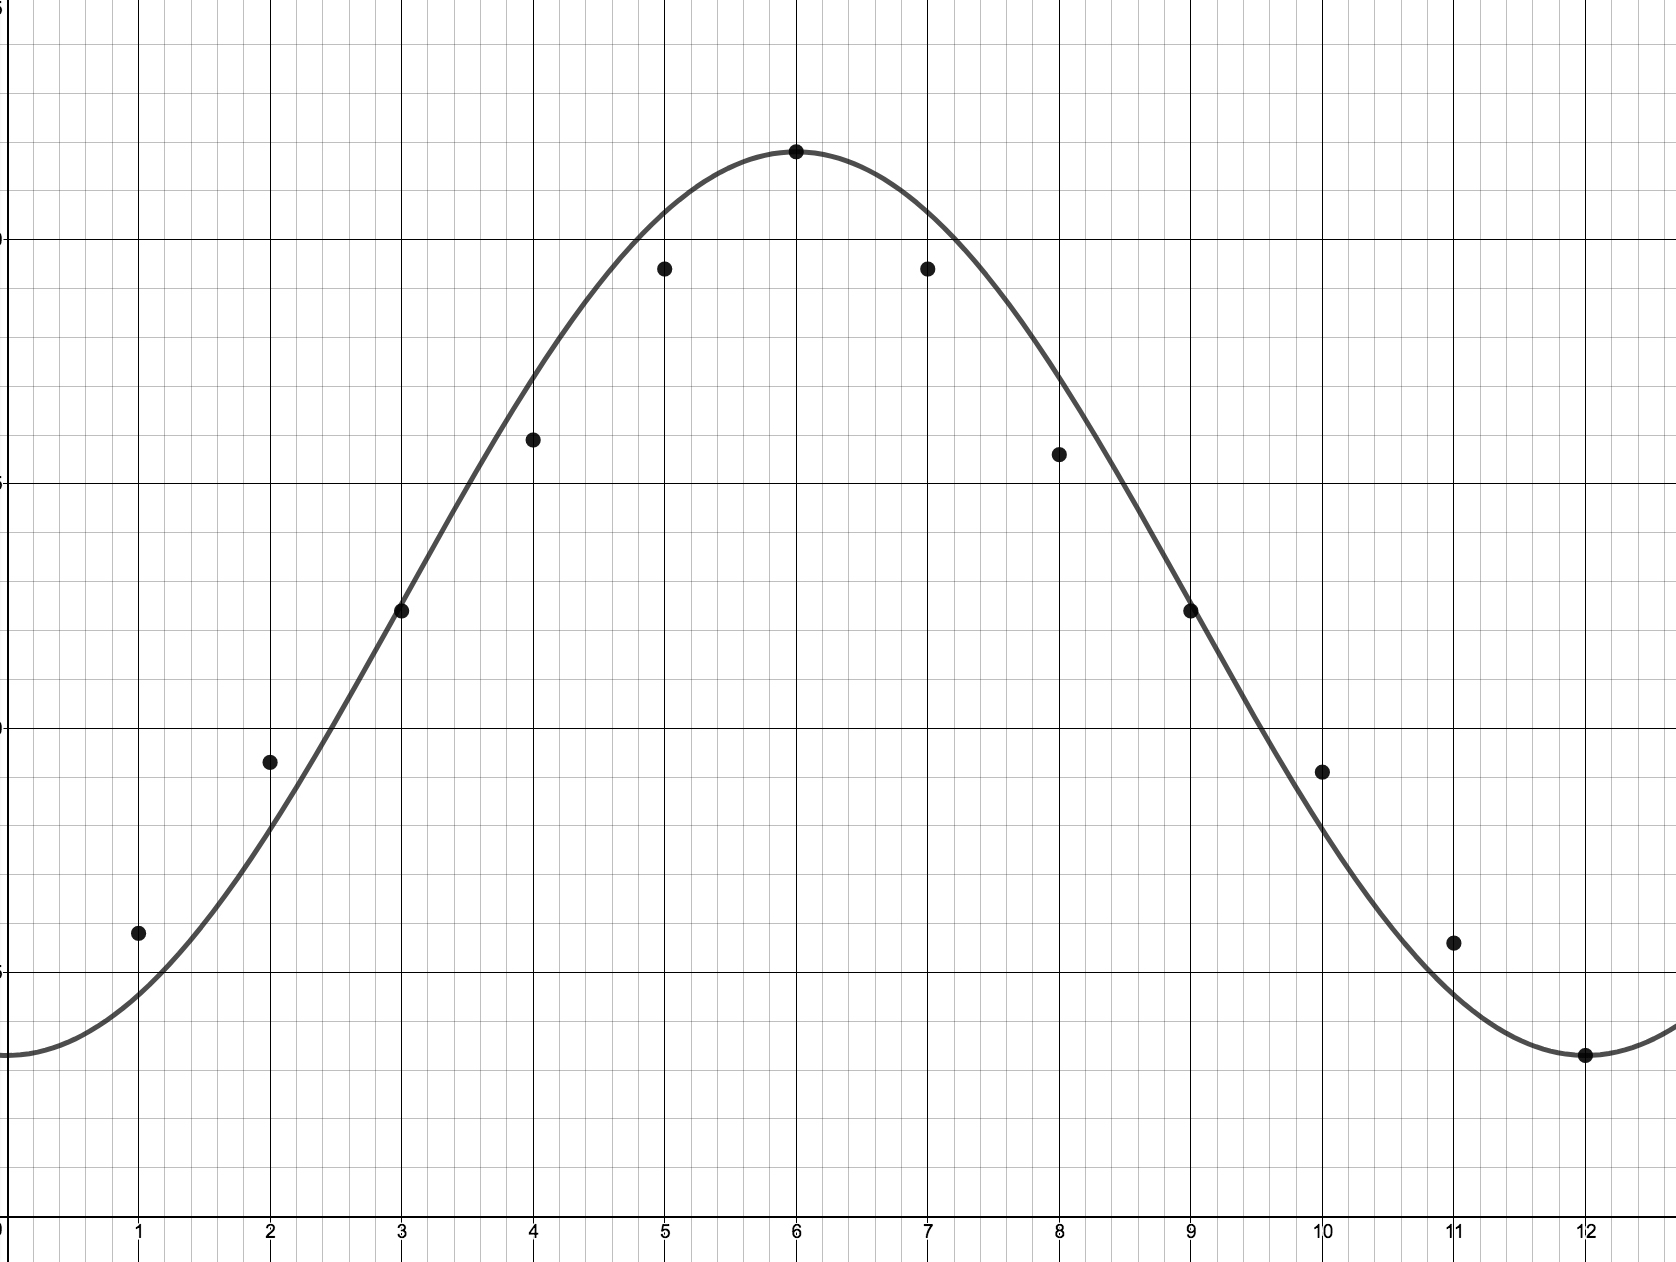
\includegraphics[height=2.5in]{./GraphsofSineandCosineGraphics/RoughFitDaylight.jpg}

\end{multicols}

\begin{multicols}{2}

Plotting the data.


Plotting the data long with $y=H(t)$


\end{multicols}

\end{center}

 
\item  Using  \href{https://www.desmos.com}{\underline{desmos}} to find a regression model produces $A \approx 8.36$ and $B \approx 12.06$, which closely match our answers from number \ref{roughsinusoidfit}. However, desmos calculates $\omega \approx -294.81$ and $\phi \approx -26.53$, which are far from our values $\omega = \frac{\pi}{6}$ and $\phi = -\frac{\pi}{2}$. 

\smallskip

Indeed, in Exercise \ref{graphdesmosregression}, we invite the reader to graph $y = 8.36 \sin(-294.81t  - 26.53) + 12.06$ using desmos.  At first glance, appears to be a solid gray rectangle. After zooming in, however, we see this rectangle is made up of literally hundreds of oscillations.  Though desmos boasts this regression as having an $R^{2}$ value of $0.9886$, meaning mathematically, this is a very good fit to the data, this curve doesn't model the real-world phenomenon of daylight hours in any sort of reasonable manner. 

\smallskip

Since we know the period of the sinusoid is 12 months, we set $\omega = \frac{\pi}{6}$ and ask desmos to run a regression for the remaining three parameters.   Desmos returns the values $A \approx -8.13$, $B \approx 12.5$, and $\phi \approx -4.70$, with an $R^{2}$ value of $0.987$,  so its regression curve is a much more reasonable $H(t) = -8.13 \sin\left(\frac{\pi}{6} t - 4.70\right)+ 12.5$.  Even though, at first glance, this curve appears much different from our solution to number \ref{roughsinusoidfit}, the we graph both functions below on the right and see they are very similar.\footnote{In Section \ref{MoreTrigonometricIdentities}, we can show how similar these two functions are analytically.  See Exercise \ref{twodaylightfunctions}.}  (Our solution to number \ref{roughsinusoidfit} is the darker of the two curves.)

\begin{center}

\begin{multicols}{2}
 

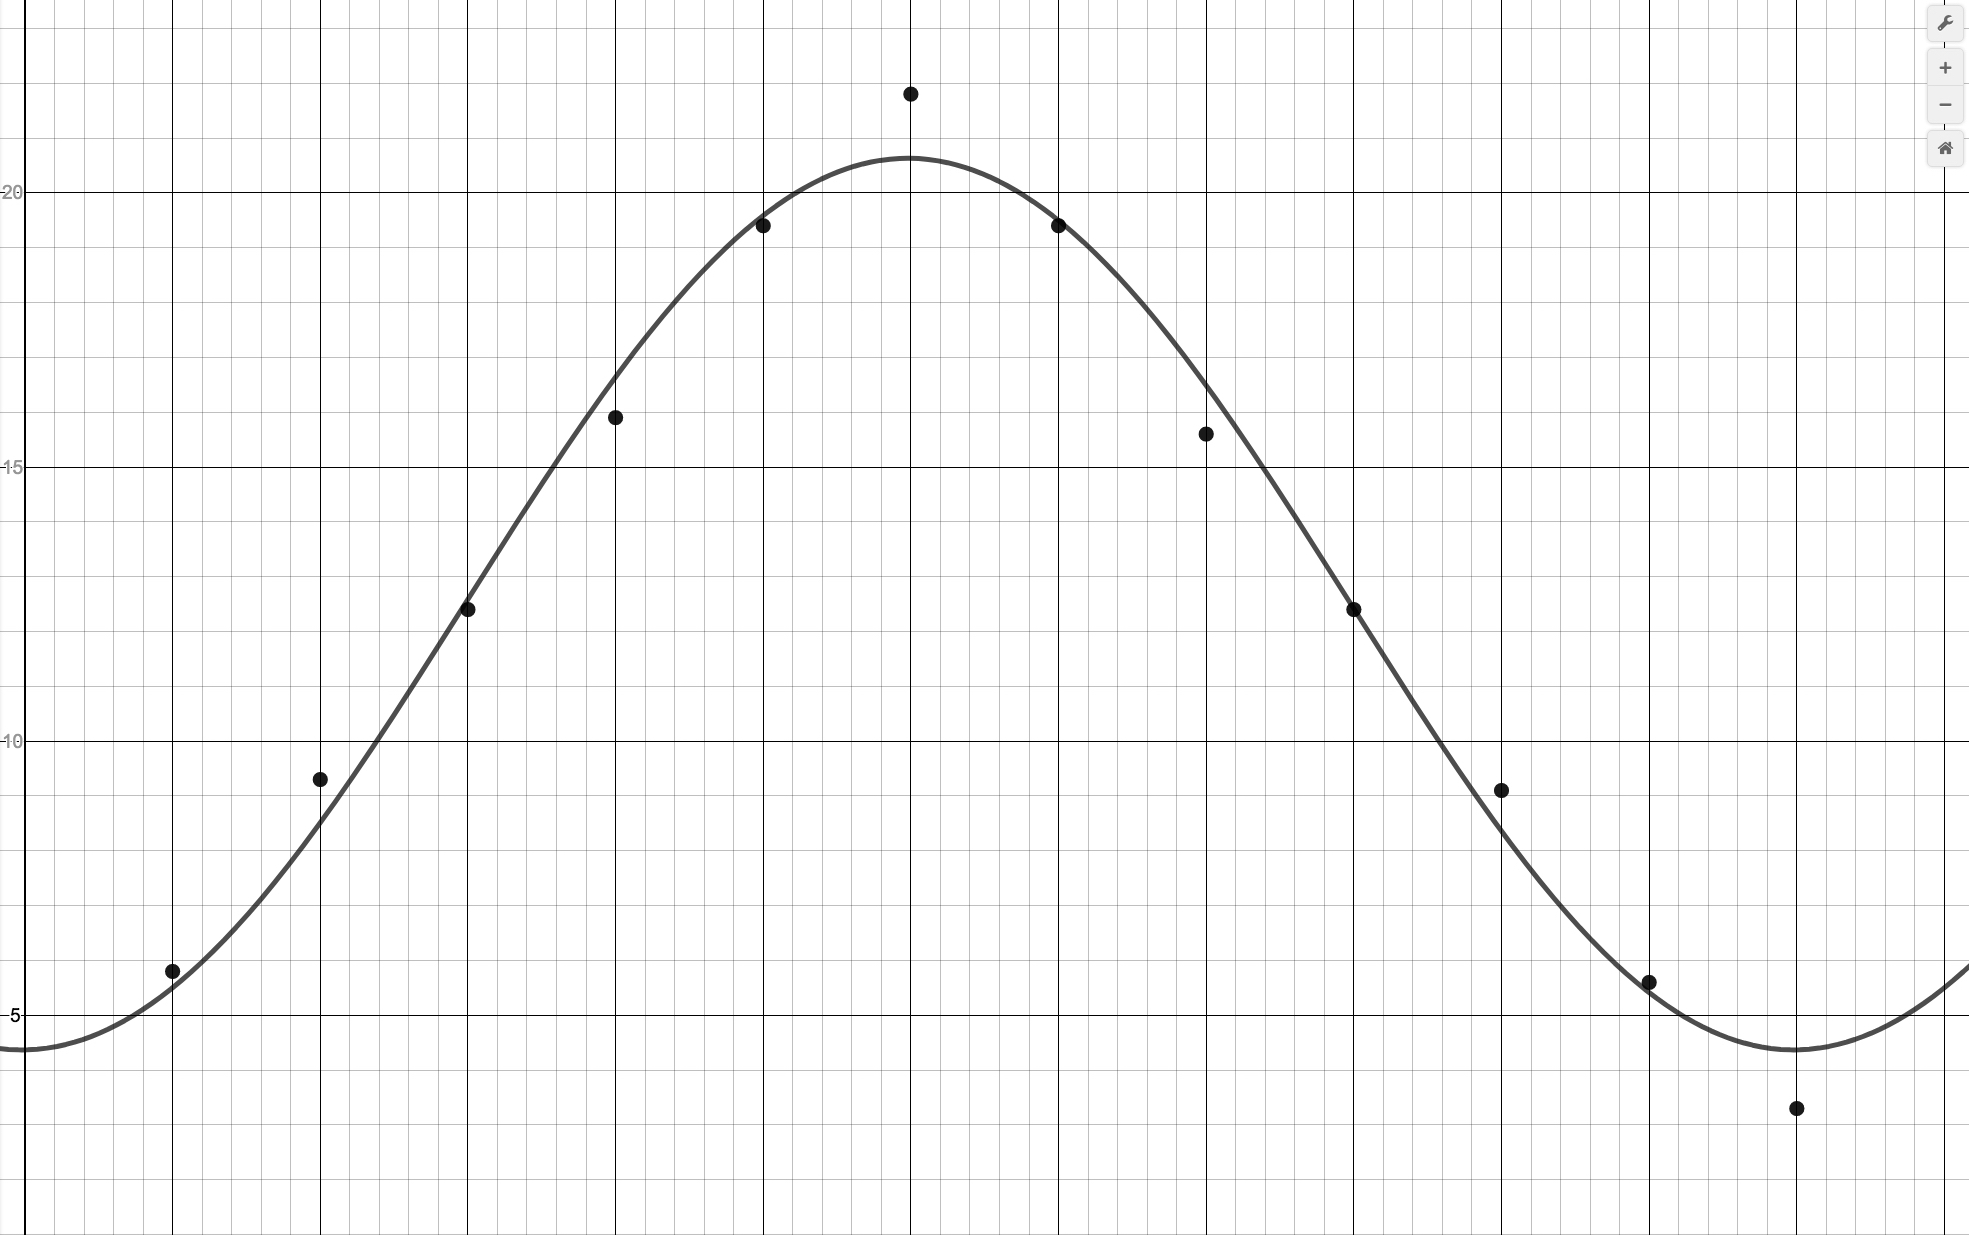
\includegraphics[width=2.75 in]{./GraphsofSineandCosineGraphics/desmos_regression.jpg}
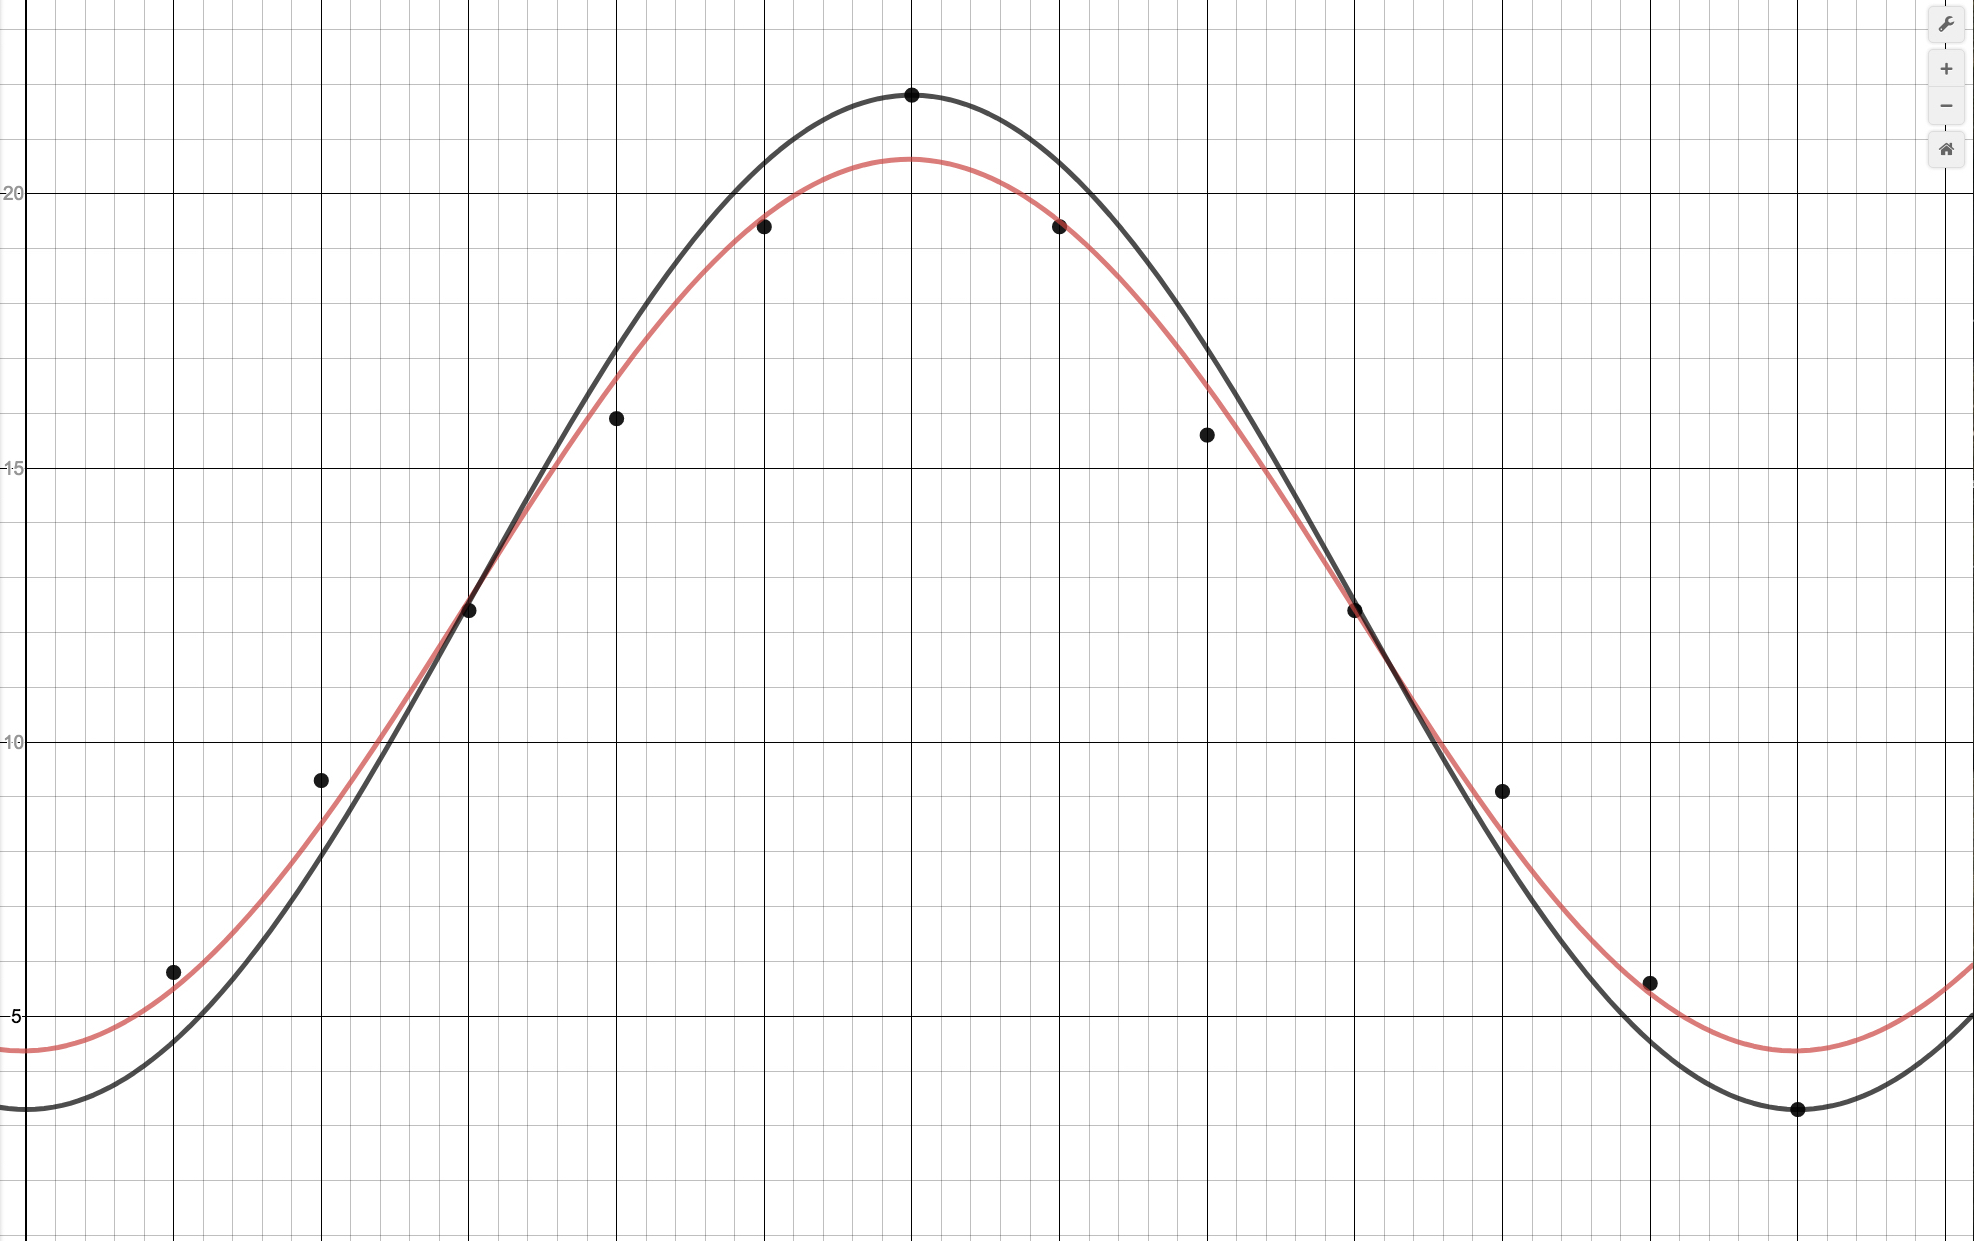
\includegraphics[width=2.75 in]{./GraphsofSineandCosineGraphics/both_daylight.jpg}
 

 
 \end{multicols}
 
 \begin{multicols}{2}

Plotting the desmos's regression curve.


Plotting both solutions.


\end{multicols}
 
 
 \end{center}
 
 \qed

\end{enumerate}

\end{ex}

The scenario described in Example \ref{sinusoidsunlight} is a typical example of where the circular functions are useful outside the context of angles or circular motion.  Indeed, sine and cosine functions are used extensively to model a wide range of periodic phenomena including signal analysis, wave physics, and even quantum mechanics.  Hence, regardless of your chosen field of study, it is well worth your time to absolutely master sinusoids.  To that end, we present the exercises.

\newpage

\subsection{Exercises}

In Exercises \ref{sinecosinegraphfirst} - \ref{sinecosinegraphlast}, graph one cycle of the given function.  State the period, amplitude, phase shift and vertical shift of the function.

\begin{multicols}{3}

\begin{enumerate}

\item $f(t) = 3\sin(t)$ \label{sinecosinegraphfirst}
\item $g(t) = \sin(3t)$
\item $h(t)  = -2\cos(t)$

\setcounter{HW}{\value{enumi}}

\end{enumerate}

\end{multicols}

\begin{multicols}{3}

\begin{enumerate}

\setcounter{enumi}{\value{HW}}

\item $f(t)  = \cos \left( t - \frac{\pi}{2} \right)$
\item $g(t)  = -\sin \left( t + \frac{\pi}{3} \right)$
\item $h(t) = \sin(2t - \pi)$ \vphantom{$\left( \frac{\pi}{2} \right)$}

\setcounter{HW}{\value{enumi}}

\end{enumerate}

\end{multicols}

\begin{multicols}{3}

\begin{enumerate}

\setcounter{enumi}{\value{HW}}

\item $f(t)  = -\frac{1}{3}\cos \left( \frac{1}{2}t + \frac{\pi}{3} \right)$
\item $g(t) = \cos (3t - 2\pi) + 4$ \vphantom{$\left( \frac{1\pi}{2} \right)$}
\item $h(t)  = \sin \left( -t - \frac{\pi}{4} \right) - 2$ \vphantom{$\left( \frac{1\pi}{2} \right)$}

\setcounter{HW}{\value{enumi}}

\end{enumerate}

\end{multicols}

\begin{multicols}{3}

\begin{enumerate}

\setcounter{enumi}{\value{HW}}

\item $f(t) = \frac{2}{3} \cos \left( \frac{\pi}{2} - 4t \right) + 1$
\item $g(t) = -\frac{3}{2} \cos \left( 2t + \frac{\pi}{3} \right) - \frac{1}{2}$
\item $h(t) = 4\sin (-2\pi t + \pi)$ \vphantom{$\left( \frac{1\pi}{2} \right)$}  \label{sinecosinegraphlast}

\setcounter{HW}{\value{enumi}}

\end{enumerate}

\end{multicols}

In Exercises \ref{fitsinecosinefirst} - \ref{fitsinecosinelast},  a sinusoid is graphed. Find a formula for the sinusoid in the form $S(t) = A \sin(\omega t + \phi) + B$ and $C(t) = A \cos(\omega t + \phi) + B$.  Select $\omega$ so  $\omega > 0$. Check your answer by graphing.

\begin{multicols}{2}
\begin{enumerate}
\setcounter{enumi}{\value{HW}}

\item $~$   \label{fitsinecosinefirst}  %$S(t) = 4 \sin \left(t + \frac{\pi}{4} \right)$, $C(t) = 4 \cos \left(t - \frac{\pi}{4} \right)$

\begin{mfpic}[16]{-5}{5}{-5}{5}
\tlabel[cc](5,-0.30){\scriptsize $t$}
\tlabel[cc](0.25,5){\scriptsize $y$}
\axes
\xmarks{-4 step 1 until 4}
\ymarks{-4 step 1 until 4}
\point[4pt]{(-3.927, 0), (-2.356, -4), (-0.7854, 0), (0.7854, 4), (2.356, 0)}
\tlabel[cc](-3, 0.5){ \scriptsize $\left( -\frac{5\pi}{4}, 0 \right)$}
\tlabel[cc](-2.356, -4.5){ \scriptsize $\left( -\frac{3\pi}{4}, -4 \right)$}
\gclear \tlabelrect(0.25, -0.6){ \scriptsize $\left( -\frac{\pi}{4}, 0 \right)$ \vphantom{$\dfrac{5}{2}$}}
\tlabel[cc](0.9, 4.5){\scriptsize $\left( \frac{\pi}{4}, 4 \right)$}
\tlabel[cc](3.25, 0.5){ \scriptsize $\left( \frac{3\pi}{4}, 4 \right)$}
\tlpointsep{4pt}
%\axislabels {x}{{$\frac{\pi}{2}$} 1.5708, {$\pi$} 3.1416, {$\frac{3\pi}{2}$} 4.7124, {$2\pi$} 6.2832}
%\axislabels {y}{{$-3$} -3, {$3$} 3}
\penwd{1.25pt}
\arrow \reverse \arrow \function{-5, 5,  0.1}{4*sin(x+(pi/4))}
\end{mfpic}   


\item$~$     % $S(t) = -3 \sin(t) + 3$, $C(t) = -3 \cos\left(t - \frac{\pi}{2}\right) + 3$

\begin{mfpic}[16]{-6}{6}{-1}{9}
\tlabel[cc](6,-0.30){\scriptsize $t$}
\tlabel[cc](0.25,9){\scriptsize $y$}
\axes
\xmarks{-5 step 1 until 5}
\ymarks{1 step 1 until 8}
\point[4pt]{(-4.712, 0), (-1.571, 6), (0,3), (1.571, 0), (4.712, 6)}
\tlabel[cc](-4.712, -0.75){\scriptsize $\left( -\frac{3\pi}{2}, 0 \right)$}
\tlabel[cc](-1.571, 6.5){\scriptsize $\left( -\frac{\pi}{2}, 6 \right)$}
\tlabel[cc](0.75, 3){ \scriptsize $\left(0, 3 \right)$}
\tlabel[cc](4.712, 6.5){\scriptsize $\left( \frac{3 \pi}{2}, 6 \right)$}
\tlabel[cc](1.571, -0.75){\scriptsize $\left( \frac{\pi}{2}, 0 \right)$}
\tlpointsep{4pt}
%\axislabels {x}{{$\frac{\pi}{2}$} 1.5708, {$\pi$} 3.1416, {$\frac{3\pi}{2}$} 4.7124, {$2\pi$} 6.2832}
%\axislabels {y}{{$-3$} -3, {$3$} 3}
\penwd{1.25pt}
\arrow \reverse \arrow \function{-6, 6,  0.1}{3- 3*sin(x)}
\end{mfpic}  

\setcounter{HW}{\value{enumi}}
\end{enumerate}
\end{multicols}

\begin{multicols}{2}
\begin{enumerate}
\setcounter{enumi}{\value{HW}}

\item $~$    %$S(t) = 3 \sin \left( 2t - \frac{\pi}{3} \right)$, $C(t) = 3 \cos \left( 2t - \frac{5\pi}{6} \right)$

\begin{mfpic}[15]{-6}{6}{-5}{5}
\tlabel[cc](6,-0.30){\scriptsize $t$}
\tlabel[cc](0.25,5){\scriptsize $y$}
\axes
\xmarks{-5 step 1 until 5}
\ymarks{-4 step 1 until 4}
\point[4pt]{(-4.974, 3), (-4.189, 0), (-3.403, -3), (-2.618, 0), (-1.832, 3), (-1.047, 0), (-0.2618, -3), (0.5236, 0), (1.309, 3), (2.094, 0), (2.8880, -3), (3.665, 0), (4.45, 3), (5.236, 0)}
\tlabel[cc](-4.974, 3.75){ \scriptsize $\left( -\frac{19 \pi}{12}, 3 \right)$}
\tlabel[cc](-3.403, -3.75){ \scriptsize $\left( -\frac{13 \pi}{12}, -3 \right)$}
\tlabel[cc] (-1.832, 3.75){ \scriptsize $\left( -\frac{7 \pi}{12}, 3 \right)$}
\gclear \tlabelrect(0, -3.75){ \scriptsize $\left( -\frac{\pi}{12}, -3 \right)$}
\tlabel[cc] (1.309, 3.75){ \scriptsize $\left( \frac{5 \pi}{12}, 3 \right)$}
\tlabel[cc](2.880, -3.75){ \scriptsize $\left( \frac{11 \pi}{12}, -3 \right)$}
\tlabel[cc] (4.45, 3.75){ \scriptsize $\left( \frac{17 \pi}{12}, 3 \right)$}

\tlpointsep{4pt}
%\axislabels {x}{{$\frac{\pi}{2}$} 1.5708, {$\pi$} 3.1416, {$\frac{3\pi}{2}$} 4.7124, {$2\pi$} 6.2832}
%\axislabels {y}{{$-3$} -3, {$3$} 3}
\penwd{1.25pt}
\arrow \reverse \arrow \function{-6, 5.5,  0.1}{3*sin((2*x)-(pi/3))}
\end{mfpic}   


\item$~$     \label{fitsinecosinelast}  % $S(t) =  \frac{7}{2} \sin(\pi t) + \frac{1}{2}$, $C(t) = \frac{7}{2} \cos\left(\pi t \frac{\pi}{2} \right) + \frac{1}{2}$

\begin{mfpic}[22][15]{-5}{5}{-5}{5}
\tlabel[cc](5,-0.30){\scriptsize $t$}
\tlabel[cc](0.25,5){\scriptsize $y$}
\axes
\xmarks{-4 step 1 until 4}
\ymarks{-4 step 1 until 4}
\point[4pt]{ (-4, 0.5), (-3.5, 4), (-3, 0.5), (-2.5, -3), (-2, 0.5), (-1.5, 4), (-1, 0.5), (-0.5, -3), (0, 0.5), (0.5, 4), (1, 0.5), (1.5,-3), (2, 0.5), (2.5,4), (3, 0.5), (3.5,-3), (4, 0.5) }
%\tlabel[cc](-4.5, -3.5){\scriptsize $(-4.5, -3)$}
\tlabel[cc](-3.5, 4.5){\scriptsize $(-3.5, 4)$}
\tlabel[cc](-2.5, -3.5){\scriptsize $(-2.5, -3)$}
\tlabel[cc](-1.5, 4.5){\scriptsize $(-1.5, 4)$}
%\tlabel[cc](-0.5, -3.5){\scriptsize $(-0.5, -3)$}
\gclear \tlabelrect(0.75, 4.5){\scriptsize $(0.5, 4)$}
\tlabel[cc](1.5, -3.5){\scriptsize $(1.5, -3)$}
\tlabel[cc](2.5, 4.5){\scriptsize $(2.5, 4)$}
%\tlabel[cc](2.5, -3.5){\scriptsize $(2.5, -3)$}
%\tlabel[cc](4.5, 4.5){\scriptsize $(4.5, 4)$}

\tlpointsep{4pt}
%\axislabels {x}{{$\frac{\pi}{2}$} 1.5708, {$\pi$} 3.1416, {$\frac{3\pi}{2}$} 4.7124, {$2\pi$} 6.2832}
%\axislabels {y}{{$-3$} -3, {$3$} 3}
\penwd{1.25pt}
\arrow \reverse \arrow \function{-4.25, 4.25,  0.1}{(3.5*sin(pi*x))+0.5}
\end{mfpic}   

\setcounter{HW}{\value{enumi}}
\end{enumerate}
\end{multicols}


\begin{enumerate}
\setcounter{enumi}{\value{HW}}

\item  Use the graph of  $S(t) = 4 \sin(t)$ to graph each of the following functions. State the period of each.

\begin{multicols}{2}

\begin{enumerate}

\item $f(t) = | 4 \sin(t)|$

\item $g(t) = \sqrt{4 \sin(t)}$

\end{enumerate}
\end{multicols}


\setcounter{HW}{\value{enumi}}
\end{enumerate}

In Exercises \ref{exploregraphsfirst} - \ref{exploregraphslast}, use a graphing utility to graph each function and discuss the related questions with your classmates.


\begin{enumerate}

\setcounter{enumi}{\value{HW}}

\item  $f(t) = \cos(3t) + \sin(t)$.  Is this function periodic?  If so, what is the period? \label{exploregraphsfirst}
\item  $f(t) = \frac{\sin(t)}{t}$.  What appears to be the horizontal asymptote of the graph? 
\item  $f(t) = t \sin(t)$.  Graph $y = \pm t$. What do you notice? 
\item  $f(t) = \sin\left(\frac{1}{t}\right)$.  What's happening as $t \rightarrow 0$?
%\item  $f(x) = x - \tan(x)$.  Graph $y = x$ on the same set of axes and describe the behavior of $f$.  
\item  $f(t) = e^{-0.1t} \left( \cos(2t) + \sin(2t)\right)$.  Graph $y = \pm e^{-0.1t}$ on the same set of axes. What do you notice?
\item  $f(t) = e^{-0.1t} \left( \cos(2t) + 2\sin(t)\right)$.  Graph $y = \pm e^{-0.1t}$ on the same set of axes.  What do you notice? \label{exploregraphslast}

\setcounter{HW}{\value{enumi}}

\end{enumerate}

\begin{enumerate}

\setcounter{enumi}{\value{HW}}

\item Show every constant function $f$ is periodic by explaining why $f(x + 117) = f(x)$ for all real numbers $x$. Then show that $f$ has no period by showing that you cannot find a \emph{smallest} number $p$ such that $f(x + p) = f(x)$ for all real numbers $x$.  

\smallskip

Said differently, show that $f(x + p) = f(x)$ for all real numbers $x$ for ALL values of $p > 0$, so no smallest value exists to satisfy the definition of `period'.

\setcounter{HW}{\value{enumi}}

\end{enumerate}

\begin{enumerate}

\setcounter{enumi}{\value{HW}}

\item  The sounds we hear are made up of mechanical waves.  The note `A' above the note `middle C' is a sound wave with ordinary frequency $f = 440$ Hertz $= 440 \frac{\text{cycles}}{\text{second}}$.  Find a sinusoid which models this note, assuming that the amplitude is $1$ and the phase shift is $0$.

\item The voltage $V$ in an alternating current source has amplitude $220 \sqrt{2}$ and ordinary frequency $f = 60$ Hertz.  Find a sinusoid which models this voltage.  Assume that the phase is $0$.


\item \label{heightlondoneye} The \href{http://en.wikipedia.org/wiki/London_Eye}{\underline{London Eye}} is a popular tourist attraction in London, England and is one of the largest Ferris Wheels in the world.  It has a diameter of 135 meters and makes one revolution (counter-clockwise) every 30 minutes.  It is constructed so that the lowest part of the Eye reaches ground level, enabling passengers to simply walk on to, and off of, the ride.  Find a sinsuoid which models the height $h$ of the passenger above the ground in meters $t$ minutes after they board the Eye at ground level.

\item \label{leftrightlondoneye} On page \pageref{equationsforcircularmotion} in Section \ref{cosinesinebeyond}, we found the $x$-coordinate of counter-clockwise motion on a circle of radius $r$ with angular frequency $\omega$ to be $x = r\cos(\omega t)$, where $t=0$ corresponds to the point $(r,0)$.  Suppose we are in the situation of Exercise \ref{heightlondoneye} above.  Find a sinsusoid which models the horizontal \textit{displacement} $x$ of the passenger from the center of the Eye in meters $t$ minutes after they board the Eye.  Here we take $x(t) > 0$ to mean the passenger is to the \textit{right} of the center, while $x(t) < 0$ means the passenger is to the \textit{left} of the center.

\item  In Exercise \ref{yoyotrick} in Section \ref{RadianMeasure}, we introduced the yo-yo trick `Around the World' in which a yo-yo is thrown so it sweeps out a vertical circle.  As in that exercise, suppose the yo-yo string is 28 inches and it completes one revolution in 3 seconds.  If the closest the yo-yo ever gets to the ground is 2 inches, find a sinsuoid which models the height $h$ of the yo-yo above the ground in inches $t$ seconds after it leaves its lowest point.



\item  Consider the pendulum below.  Ignoring air resistance, the angular displacement of the pendulum from the vertical position, $\theta$, can be modeled as a sinusoid.\footnote{Provided $\theta$ is kept `small.'  Carl remembers the `Rule of Thumb' as being $20^{\circ}$ or less.  Check with your friendly neighborhood physicist to make sure.}


\begin{center}

\begin{mfpic}[15]{-3}{3}{-5}{1}
\polyline{(0,0), (0,-5)}
\dashed \polyline{(0,0), (2.5, -4.33)}
\arrow \parafcn{275, 295, 5}{4*dir(t)}
\tlabel[cc](1.29, -4.83){$\theta$}
\hatchcolor[gray]{.7}
\lhatch \rect{(-3,0), (3,1)}
\fillcolor[gray]{.7} 
\gfill \circle{(0,-5),0.25}
\gfill \circle{(2.5, -4.33),0.20}
\penwd{1.025}
\circle{(0,-5),0.25}
\circle{(2.5, -4.33),0.25}
\rect{(-3,0), (3,1)}
\end{mfpic} 
\end{center}

The amplitude of the sinusoid is the same as the initial angular displacement, $\theta_{\text{\tiny $0$}}$, of the pendulum and the  period of the motion is given by

\[T = 2\pi \sqrt{\dfrac{\ell}{g}}\]

where $\ell$ is the length of the pendulum and $g$ is the acceleration due to gravity.

\begin{enumerate}

\item  Find a sinusoid which gives the angular displacement $\theta$ as a function of time, $t$. Arrange things so $\theta(0) = \theta_{\text{\tiny $0$}}$.

\item  In Exercise \ref{pendulumproblem} section \ref{RootRadicalFunctions}, you found the length of the pendulum needed in Jeff's antique Seth-Thomas clock to ensure the period of the pendulum is $\frac{1}{2}$ of a second. Assuming the initial displacement of the pendulum is $15^{\circ}$, find a sinusoid which models the displacement of the pendulum $\theta$ as a function of time, $t$, in seconds. 

\end{enumerate}

\newpage

\item  The table below lists the average temperature of Lake Erie as measured in Cleveland, Ohio on the first of the month for each month during the years 1971 -- 2000.\footnote{See this website: \href{http://www.erh.noaa.gov/cle/climate/cle/normals/laketempcle.html}{\underline{http://www.erh.noaa.gov/cle/climate/cle/normals/laketempcle.html}.}}  For example,   $t=3$ represents the average of the temperatures recorded for Lake Erie on every March 1 for the years 1971 -- 2000.

\medskip

\small

\noindent \begin{tabular}{|l|r|r|r|r|r|r|r|r|r|r|r|r|} \hline
Month  & & & & & & & & & & & & \\
Number, $t$ & 1 & 2 & 3 & 4 & 5 & 6 & 7 & 8 & 9 & 10 & 11 & 12\\ 
\hline 
Temperature  & & & & & & & & & & & & \\
($^{\circ}$ F), $T$ & 36 & 33 & 34 & 38 & 47 & 57 & 67 & 74 & 73 & 67 & 56 & 46 \\ \hline
\end{tabular}

\normalsize

\medskip

\begin{enumerate}

\item \label{LakeErieTempData} Using the techniques discussed in Example \ref{sinusoidsunlight}, fit a sinusoid to these data. 

\item  Graph your model along with the data set to judge the reasonableness of the fit.

\item Use the model from \ref{LakeErieTempData} to predict the average temperature recorded for Lake Erie on April $15^{\text{th}}$ and September $15^{\text{th}}$ during the years 1971--2000.\footnote{The computed average is $41^{\circ}$F for April $15^{\text{th}}$ and $71^{\circ}$F for September $15^{\text{th}}$.}

\item Compare your results to those obtained using a graphing utility.

\end{enumerate}

\item  The fraction of the moon illuminated at midnight Eastern Standard Time on the $t^{\text{th}}$ day of June, 2009 is given in the table below.\footnote{See this website: \href{http://www.usno.navy.mil/USNO/astronomical-applications/data-services/frac-moon-ill}{\underline{http://www.usno.navy.mil/USNO/astronomical-applications/data-services/frac-moon-ill}.}} 


\medskip

\small

\noindent \begin{tabular}{|l|r|r|r|r|r|r|r|r|r|r|} \hline
Day of  & & & & & & & & & & \\
June, $t$ & 3 & 6 & 9 & 12 & 15 & 18 & 21 & 24 & 27 & 30\\ 
\hline 
Fraction  & & & & & & & & & & \\
Illuminated, $F$ & 0.81 & 0.98 & 0.98 & 0.83 & 0.57 & 0.27 & 0.04 & 0.03 & 0.26 & 0.58  \\ \hline
\end{tabular}

\normalsize

\medskip

\begin{enumerate}

\item \label{MoonIllumination} Using the techniques discussed in Example \ref{sinusoidsunlight}, fit a sinusoid to these data.\footnote{You may want to plot the data before you find the phase shift.} 

\item  Graph your model along with the data set to judge the reasonableness of the fit.

\item Use the model from \ref{MoonIllumination} to predict the fraction of the moon illuminated on June 1, 2009. \footnote{The listed fraction is $0.62$.}

\item Compare your results to those obtained using a graphing utility.

\end{enumerate}


\item \label{graphdesmosregression}  Use a graphing utility to graph $y = 8.36 \sin(-294.81t  - 26.53) + 12.06$.  (This is the regression model produced by desmos in Example \ref{sinusoidsunlight}.) Zoom in, as needed, until you start to see the wave-like nature of the graph.  Use Theorem \ref{sinusoidform} to determine a window which produces exactly one complete cycle of this sinusoid and check your answer graphically.

\item   \label{proofsinusoidformexercise} Use Theorem \ref{transformationsthm} to prove Theorem \ref{sinusoidform}.


\item  With the help of your classmates, research \href{http://en.wikipedia.org/wiki/Amplitude_modulation}{\underline{Amplitude Modulation}} and \href{http://en.wikipedia.org/wiki/Frequency_modulation}{\underline{Frequency Modulation}}.

\item What other things in the world might be roughly sinusoidal?  Look to see what models you can find for them and share your results with your class.

\end{enumerate}

\newpage


\subsection{Answers}

\begin{enumerate}

\item \begin{multicols}{2} \raggedcolumns
$f(t) = 3\sin(t)$\\
Period: $2\pi$\\
Amplitude: $3$\\
Phase Shift: $0$\\
Vertical Shift: $0$\\

\begin{mfpic}[25][15]{-0.25}{7}{-3.5}{3.75}
\point[4pt]{(0,0), (1.5708,3), (3.1416, 0), (4.7124,-3), (6.2832,0)}
\axes
\tlabel[cc](7,-0.30){$t$}
\tlabel[cc](0.25,3.75){$y$}
\xmarks{1.5708, 3.1416, 4.7124, 6.2832 }
\ymarks{-3,3}
\tlpointsep{4pt}
\axislabels {x}{{$\frac{\pi}{2}$} 1.5708, {$\pi$} 3.1416, {$\frac{3\pi}{2}$} 4.7124, {$2\pi$} 6.2832}
\axislabels {y}{{$-3$} -3, {$3$} 3}
\penwd{1.25pt}
\function{0, 6.2832, 0.1}{3*sin(x)}
\end{mfpic}

\end{multicols}

\item \begin{multicols}{2} \raggedcolumns
$g(t)  = \sin(3t)$\\
Period: $\frac{2\pi}{3}$\\
Amplitude: $1$\\
Phase Shift: $0$\\
Vertical Shift: $0$\\

\begin{mfpic}[70][50]{-0.25}{2.5}{-1.25}{1.25}
\point[4pt]{(0,0), (0.5236,1), (1.0472,0), (1.5708,-1), (2.0944,0)}
\axes
\tlabel[cc](2.5,-0.15){$t$}
\tlabel[cc](0.15,1.25){$y$}
\xmarks{0.5236, 1.0472, 1.5708, 2.0944}
\ymarks{-1,1}
\tlpointsep{4pt}
\axislabels {x}{{$\frac{\pi}{6}$} 0.5236, {$\frac{\pi}{3}$} 1.0472, {$\frac{\pi}{2}$} 1.5708, {$\frac{2\pi}{3}$} 2.0944}
\axislabels {y}{{$-1$} -1, {$1$} 1}
\penwd{1.25pt}
\function{0, 2.0944, 0.1}{sin(3*x)}
\end{mfpic}

\end{multicols}

\item \begin{multicols}{2} \raggedcolumns
$h(t) = -2\cos(t)$\\
Period: $2\pi$\\
Amplitude: $2$\\
Phase Shift: $0$\\
Vertical Shift: $0$\\

\begin{mfpic}[25]{-0.25}{7}{-2.5}{2.5}
\point[4pt]{(0,-2), (1.5708,0), (3.1416, 2), (4.7124,0), (6.2832,-2)}
\axes
\tlabel[cc](7,-0.25){$t$}
\tlabel[cc](0.25,2.5){$y$}
\xmarks{1.5708, 3.1416, 4.7124, 6.2832}
\ymarks{-2,2}
\tlpointsep{4pt}
\axislabels {x}{{$\frac{\pi}{2}$} 1.5708, {$\pi$} 3.1416, {$\frac{3\pi}{2}$} 4.7124, {$2\pi$} 6.2832}
\axislabels {y}{{$-2$} -2, {$2$} 2}
\penwd{1.25pt}
\function{0, 6.2832, 0.1}{-2*cos(x)}
\end{mfpic}

\end{multicols}

\item \begin{multicols}{2} \raggedcolumns
$f(t) = \cos \left( t - \frac{\pi}{2} \right)$\\
Period: $2\pi$\\
Amplitude: $1$\\
Phase Shift: $\frac{\pi}{2}$\\
Vertical Shift: $0$\\

\begin{mfpic}[22][40]{-0.25}{8.3}{-1.5}{1.5}
\point[4pt]{(1.5708,1), (3.1416, 0), (4.7124,-1), (6.2832,0), (7.854,1)}
\axes
\tlabel[cc](8.3,-0.25){$t$}
\tlabel[cc](0.25,1.5){$y$}
\xmarks{1.5708, 3.1416, 4.7124, 6.2832, 7.854}
\ymarks{-1,1}
\tlpointsep{4pt}
\axislabels {x}{{$\frac{\pi}{2}$} 1.5708, {$\pi$} 3.1416, {$\frac{3\pi}{2}$} 4.7124, {$2\pi$} 6.2832, {$\frac{5\pi}{2}$} 7.854}
\axislabels {y}{{$-1$} -1, {$1$} 1}
\penwd{1.25pt}
\function{1.5708, 7.854, 0.1}{cos(x - 1.5708)}
\end{mfpic}

\end{multicols}


\item \begin{multicols}{2} \raggedcolumns
$g(t) = -\sin \left( t + \frac{\pi}{3} \right)$\\
Period: $2\pi$\\
Amplitude: $1$\\
Phase Shift: $-\frac{\pi}{3}$\\
Vertical Shift: $0$\\

\begin{mfpic}[27][40]{-1.25}{5.75}{-1.5}{1.5}
\point[4pt]{(-1.0472,0), (0.5236,-1), (2.0944,0), (3.6652,1), (5.236,0)}
\axes
\tlabel[cc](5.75,-0.25){$t$}
\tlabel[cc](0.25,1.5){$y$}
\xmarks{-1.0472, 0.5236, 2.0944, 3.6652, 5.236}
\ymarks{-1,1}
\tlpointsep{4pt}
\axislabels {x}{{$-\frac{\pi}{3}$} -1.0472, {$\frac{\pi}{6}$} 0.5236, {$\frac{2\pi}{3}$} 2.0944, {$\frac{7\pi}{6}$} 3.6652, {$\frac{5\pi}{3}$} 5.236}
\axislabels {y}{{$-1$} -1, {$1$} 1}
\penwd{1.25pt}
\function{-1.0472, 5.236, 0.1}{-sin(x + 1.0472)}
\end{mfpic}

\end{multicols}

\item \begin{multicols}{2} \raggedcolumns
$h(t) = \sin(2t - \pi)$\\
Period: $\pi$\\
Amplitude: $1$\\
Phase Shift: $\frac{\pi}{2}$\\
Vertical Shift: $0$\\

\begin{mfpic}[35][50]{0}{5.25}{-1.15}{1.5}
\point[4pt]{(1.5708,0), (2.3562,1), (3.1415,0), (3.927,-1), (4.7124,0)}
\axes
\tlabel[cc](5.25,-0.25){$t$}
\tlabel[cc](0.25,1.5){$y$}
\xmarks{1.5708, 2.3562, 3.1415, 3.927, 4.7124}
\ymarks{-1,1}
\tlpointsep{4pt}
\axislabels {x}{{$\frac{\pi}{2}$} 1.5708, {$\frac{3\pi}{4}$} 2.3562, {$\pi$} 3.1415, {$\frac{5\pi}{4}$} 3.927, {$\frac{3\pi}{2}$} 4.7124}
\axislabels {y}{{$-1$} -1, {$1$} 1}
\penwd{1.25pt}
\function{1.5708, 4.7124, 0.1}{sin(2*x - 3.1415)}
\end{mfpic}

\end{multicols}

\item \begin{multicols}{2} \raggedcolumns
$f(t)  = -\frac{1}{3}\cos \left( \frac{1}{2}t  + \frac{\pi}{3} \right)$\\
Period: $4\pi$\\
Amplitude: $\frac{1}{3}$\\
Phase Shift: $-\frac{2\pi}{3}$\\
Vertical Shift: $0$\\

\begin{mfpic}[14][100]{-2.25}{11.5}{-0.5}{0.5}
\point[4pt]{(-2.0944, -0.3333), (1.0472, 0), (4.1888, 0.3333), (7.3304, 0), (10.472, -0.3333)}
\axes
\tlabel[cc](11.5,-0.05){$t$}
\tlabel[cc](0.25,0.5){$y$}
\xmarks{-2.0944, 1.0472, 4.1888, 7.3304, 10.472}
\ymarks{-0.3333, 0.3333}
\tlpointsep{4pt}
\axislabels {x}{{$-\frac{2\pi}{3}$} -2.0944, {$\frac{\pi}{3}$} 1.0472, {$\frac{4\pi}{3}$} 4.1888, {$\frac{7\pi}{3}$} 7.3304, {$\frac{10\pi}{3}$} 10.472}
\axislabels {y}{{$-\frac{1}{3}$} -0.3333, {$\frac{1}{3}$} 0.3333}
\penwd{1.25pt}
\function{-2.0944, 10.472, 0.1}{-0.3333*cos(0.5*x + 1.0472)}
\end{mfpic}

\end{multicols}

\item \begin{multicols}{2} \raggedcolumns
$g(t) = \cos (3t - 2\pi) + 4$\\
Period: $\frac{2\pi}{3}$\\
Amplitude: $1$\\
Phase Shift:  $\frac{2\pi}{3}$\\
Vertical Shift: 4\\

\begin{mfpic}[36][25]{-0.5}{5}{-0.5}{5.5}
\point[4pt]{(2.0944,5), (2.618,4), (3.1415,3), (3.6652,4), (4.1888,5)}
\axes
\tlabel[cc](5,-0.25){$t$}
\tlabel[cc](0.25,5.5){$y$}
\xmarks{2.0944, 2.618, 3.1415, 3.6652, 4.1888}
\ymarks{3,4,5}
\tlpointsep{4pt}
\axislabels {x}{{$\frac{2\pi}{3}$} 2.0944, {$\frac{5\pi}{6}$} 2.618, {$\pi$} 3.1415, {$\frac{7\pi}{6}$} 3.6652, {$\frac{4\pi}{3}$} 4.1888}
\axislabels {y}{{$3$} 3, {$4$} 4, {$5$} 5}
\penwd{1.25pt}
\function{2.0944, 4.1888, 0.1}{cos(3*x - 6.2834) + 4}
\end{mfpic}

\end{multicols}

\item \begin{multicols}{2} \raggedcolumns
$h(t) = \sin \left( -t - \frac{\pi}{4} \right) - 2$ \\
Period: $2\pi$\\
Amplitude: $1$\\
Phase Shift: $-\frac{\pi}{4}$ (You need to use \\ \vspace*{.1in}
$y = -\sin \left( t + \frac{\pi}{4} \right) - 2 $ to find this.)\footnote{Two cycles of the graph are shown to illustrate the discrepancy discussed on page \pageref{phaseshiftissue}.}\\
Vertical Shift: $-2$\\

\begin{mfpic}[13][27]{-7.5}{6.5}{-3.25}{0.5}
\point[4pt]{(-7.0686,-2), (-5.4979,-3), (-3.927,-2), (-2.3562,-1), (-0.7854,-2), (0.7854,-3), (2.3562,-2), (3.927,-1), (5.4979,-2)}
\axes
\tlabel[cc](6.5,-0.25){$t$}
\tlabel[cc](0.25,0.5){$y$}
\xmarks{-7.0686, -5.4979, -3.927, -2.3562,-0.7854, 0.7854, 2.3562, 3.927, 5.4979}
\ymarks{-3,-2,-1}
\tlpointsep{5pt}
\axislabels {x}{{$-\frac{9\pi}{4} \hspace{6pt}$} -7.0686, {$-\frac{7\pi}{4} \hspace{6pt}$} -5.4979, {$-\frac{5\pi}{4} \hspace{6pt}$} -3.927, {$-\frac{3\pi}{4} \hspace{6pt}$} -2.3562, {$-\frac{\pi}{4} \hspace{6pt}$} -0.7854, {$\frac{\pi}{4}$} 0.7854, {$\frac{3\pi}{4}$} 2.3562, {$\frac{5\pi}{4}$} 3.927, {$\frac{7\pi}{4}$} 5.4979}
\axislabels {y}{{$-3$} -3, {$-2$} -2, {$-1$} -1}
\penwd{1.25pt}
\function{-7.0686, 5.4979, 0.1}{-1*sin(x + 0.7854) - 2}
\end{mfpic}

\end{multicols}

\item \begin{multicols}{2} \raggedcolumns
$f(t) = \frac{2}{3} \cos \left( \frac{\pi}{2} - 4t \right) + 1$\\ 
Period: $\frac{\pi}{2}$\\
Amplitude: $\frac{2}{3}$\\ 
Phase Shift: $\frac{\pi}{8}$ (You need to use \\
$y = \frac{2}{3} \cos \left( 4t - \frac{\pi}{2} \right) + 1$ to find this.)\footnote{Again, we graph two cycles to illustrate the discrepancy discussed on page \pageref{phaseshiftissue}.}\\
Vertical Shift: $1$\\

\begin{mfpic}[52][45]{-1.5}{2.25}{-0.25}{2}
\point[4pt]{(-1.1781, 1.6667), (-0.7854, 1), (-0.3927, 0.3333), (0, 1), (0.3927, 1.6667), (0.7854, 1), (1.1781, 0.3333), (1.5708, 1), (1.9635, 1.6667)}
\axes
\tlabel[cc](2.25,-0.25){$t$}
\tlabel[cc](0.15,2){$y$}
\xmarks{-1.1781, -0.7854, -0.3927, 0.3927, 0.7854, 1.1781, 1.5708, 1.9635}
\ymarks{0.3333, 1, 1.6667}
\tlpointsep{4pt}
\axislabels {x}{{$-\frac{3\pi}{8} \hspace{6pt}$} -1.1781, {$-\frac{\pi}{4} \hspace{6pt}$} -0.7854, {$-\frac{\pi}{8} \hspace{6pt}$} -0.3927, {$\frac{\pi}{8}$} 0.3927, {$\frac{\pi}{4}$} 0.7854, {$\frac{3\pi}{8}$} 1.1781, {$\frac{\pi}{2}$} 1.5708, {$\frac{5\pi}{8}$} 1.9635}
\axislabels {y}{{$\frac{1}{3}$} 0.333, {$1$} 1, {$\frac{5}{3}$} 1.6667}
\penwd{1.25pt}
\function{-1.1781, 1.9635, 0.1}{0.6667*cos(4*x - 1.5708) + 1}
\end{mfpic}

\end{multicols}

\item \begin{multicols}{2} \raggedcolumns
$g(t)  = -\frac{3}{2} \cos \left( 2t + \frac{\pi}{3} \right) - \frac{1}{2}$\\
Period: $\pi$\\
Amplitude: $\frac{3}{2}$\\
Phase Shift: $-\frac{\pi}{6}$\\
Vertical Shift: $-\frac{1}{2}$\\

\begin{mfpic}[51][30]{-.75}{3}{-2.25}{1.5}
\point[4pt]{(-0.5236,-2), (0.2618,-0.5), (1.0472, 1), (1.8326, -0.5), (2.618, -2)}
\axes
\tlabel[cc](3,-0.25){$t$}
\tlabel[cc](0.15,1.5){$y$}
\xmarks{-0.5236, 0.2618, 1.0472, 1.8326, 2.618}
\ymarks{-2, -0.5, 1}
\tlpointsep{4pt}
\axislabels {x}{{$-\frac{\pi}{6}$} -0.5236, {$\frac{\pi}{12}$} 0.2618, {$\frac{\pi}{3}$} 1.0472, {$\frac{7\pi}{12}$} 1.8326, {$\frac{5\pi}{6}$} 2.618}
\axislabels {y}{{$-2$} -2, {$-\frac{1}{2}$} -0.5, {$1$} 1}
\penwd{1.25pt}
\function{-0.5236, 2.618, 0.1}{-1.5*cos(2*x + 1.047) - 0.5}
\end{mfpic}

\end{multicols}

\item \begin{multicols}{2} \raggedcolumns
$h(t) = 4\sin (-2\pi t + \pi)$ \\
Period: $1$\\
Amplitude: $4$\\
Phase Shift: $\frac{1}{2}$ (You need to use \\
$h(t) =  -4\sin (2\pi t - \pi)$ to find this.)\footnote{This will be the last time we graph two cycles to illustrate the discrepancy discussed on page \pageref{phaseshiftissue}.}\\
Vertical Shift: $0$\\

\begin{mfpic}[80][12]{-.75}{1.75}{-4.5}{4.75}
\point[4pt]{(-0.5,0), (-0.25,-4), (0,0), (0.25,4), (0.5,0), (0.75,-4), (1,0), (1.25,4), (1.5,0)}
\axes
\tlabel[cc](1.75,-0.5){$t$}
\tlabel[cc](0.1,4.75){$y$}
\xmarks{-0.5, -0.25, 0.25, 0.5, 0.75, 1, 1.25, 1.5}
\ymarks{-4,4}
\tlpointsep{4pt}
\axislabels {x}{{$-\frac{1}{2}$ \hspace{6pt}} -0.5, {$-\frac{1}{4}$ \hspace{6pt}} -0.25, {$\frac{1}{4}$} 0.25, {$\frac{1}{2}$} 0.5, {$\frac{3}{4}$} 0.75, {$1$} 1, {$\frac{5}{4}$} 1.25, {$\frac{3}{2}$} 1.5}
\axislabels {y}{{$-4$} -4, {$4$} 4}
\penwd{1.25pt}
\function{-0.5, 1.5, 0.01}{(-4)*sin((6.2831853*x) - 3.14159265)}
\end{mfpic}

\end{multicols}
\setcounter{HW}{\value{enumi}}
\end{enumerate}

\begin{multicols}{2}
\begin{enumerate}
\setcounter{enumi}{\value{HW}}

\item $S(t) = 4 \sin \left(t + \frac{\pi}{4} \right)$, $C(t) = 4 \cos \left(t - \frac{\pi}{4} \right)$

\item $S(t) = -3 \sin(t) + 3$, $C(t) = -3 \cos\left(t - \frac{\pi}{2}\right) + 3$

\setcounter{HW}{\value{enumi}}
\end{enumerate}
\end{multicols}

\begin{multicols}{2}
\begin{enumerate}
\setcounter{enumi}{\value{HW}}

\item $S(t) = 3 \sin \left( 2t - \frac{\pi}{3} \right)$, $C(t) = 3 \cos \left( 2t - \frac{5\pi}{6} \right)$

\item $S(t) =  \frac{7}{2} \sin(\pi t) + \frac{1}{2}$, $C(t) = \frac{7}{2} \cos\left(\pi t \frac{\pi}{2} \right) + \frac{1}{2}$

\setcounter{HW}{\value{enumi}}
\end{enumerate}
\end{multicols}

\begin{enumerate}
\setcounter{enumi}{\value{HW}}

\item 

\begin{multicols}{2}
\begin{enumerate}


\item $y = |4 \sin(t)|$.  Period: $\pi$. \\

Two cycles are graphed below. \\

\begin{mfpic}[25][15]{-0.25}{7}{-4.5}{4.75}
\point[4pt]{(0,0), (1.5708,4), (3.1416, 0), (4.7124,4), (6.2832,0)}
\axes
\tlabel[cc](7,-0.30){$t$}
\tlabel[cc](0.25,4.75){$y$}
\xmarks{1.5708, 3.1416, 4.7124, 6.2832 }
\ymarks{4, -4}
\tlpointsep{4pt}
\axislabels {x}{{$\frac{\pi}{2}$} 1.5708, {$\pi$} 3.1416, {$\frac{3\pi}{2}$} 4.7124, {$2\pi$} 6.2832}
\axislabels {y}{{$4$} 4, {$-4$} -4}
\dotted \function{0, 6.2832, 0.1}{4*sin(x)}
\penwd{1.25pt}
\function{0, 3.14159, 0.1}{4*sin(x)}
\function{3.14159,6.2832, 0.1}{-4*sin(x)}
\end{mfpic}

\vfill

\columnbreak

\item $y = \sqrt{4 \sin(t)}$.  Period: $2\pi$. \\

One cycle is graphed below. \\


\begin{mfpic}[25][15]{-0.25}{7}{-4.5}{4.75}
\point[4pt]{(0,0), (1.5708,2), (3.1416, 0)}
\axes
\tlabel[cc](7,-0.30){$t$}
\tlabel[cc](0.25,4.75){$y$}
\xmarks{1.5708, 3.1416, 4.7124, 6.2832 }
\ymarks{2,4, -4}
\tlpointsep{4pt}
\axislabels {x}{{$\frac{\pi}{2}$} 1.5708, {$\pi$} 3.1416, {$\frac{3\pi}{2}$} 4.7124, {$2\pi$} 6.2832}
\axislabels {y}{ {$4$} 4, {$2$} 2, {$-4$} -4}
\dotted \function{0, 6.2832, 0.1}{4*sin(x)}
\penwd{1.25pt}
\function{0, 3.14159, 0.1}{sqrt(4*sin(x))}
\end{mfpic}

\end{enumerate}

\end{multicols}

\setcounter{HW}{\value{enumi}}
\end{enumerate}

\begin{enumerate}
\setcounter{enumi}{\value{HW}}
\addtocounter{enumi}{7}

\begin{multicols}{2}

\item  $S(t) = \sin\left(880\pi t\right)$

\item  $V(t) = 220 \sqrt{2} \sin\left(120\pi t\right)$

\end{multicols}


\begin{multicols}{2}

\item  $h(t) = 67.5 \sin\left(\frac{\pi}{15} t - \frac{\pi}{2} \right) + 67.5$

\item  $x(t) = 67.5 \cos\left(\frac{\pi}{15} t - \frac{\pi}{2} \right) = 67.5 \sin\left(\frac{\pi}{15} t \right)$

\end{multicols}

\item  $h(t) = 28\sin\left(\frac{2\pi}{3} t - \frac{\pi}{2}\right) + 30$


\item  \begin{multicols}{2}

\begin{enumerate}

\item  $\theta(t) = \theta_{\text{\tiny $0$}} \sin\left(\sqrt{\frac{g}{l}}\, t + \frac{\pi}{2}\right)$

\item  $\theta(t) = \frac{\pi}{12} \sin\left(4\pi t + \frac{\pi}{2}\right)$
\end{enumerate}
\end{multicols}

\item  \begin{enumerate} \item  $T(t) = 20.5 \sin\left(\frac{\pi}{6} t - \pi\right) + 53.5$ 

\item  The model and data are graphed below.  The sinusoid is shifted to the right of our data.

\begin{center}

 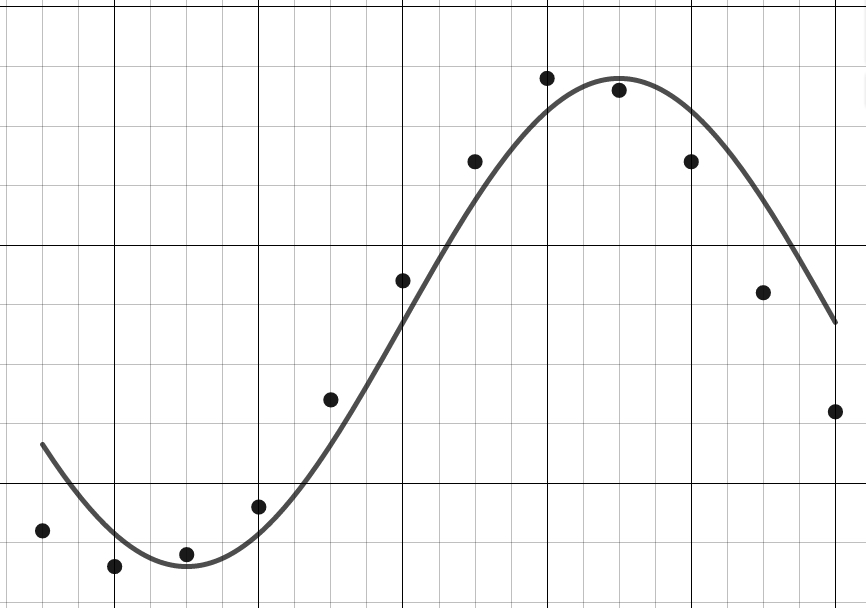
\includegraphics[height=1.5in]{./GraphsofSineandCosineGraphics/LakeErieTempReg.jpg} 

\end{center}

\item The average temperature on April $15^{\text{th}}$ is approximately $T(4.5) \approx 39.00^{\circ}$F and the average temperature on September $15^{\text{th}}$ is approximately $T(9.5) \approx 73.38^{\circ}$F.

\item  Desmos gives: $T(t) = 20.8374 \sin (-0.5251 t-0.2812) +52.3659$.  


\begin{center}

 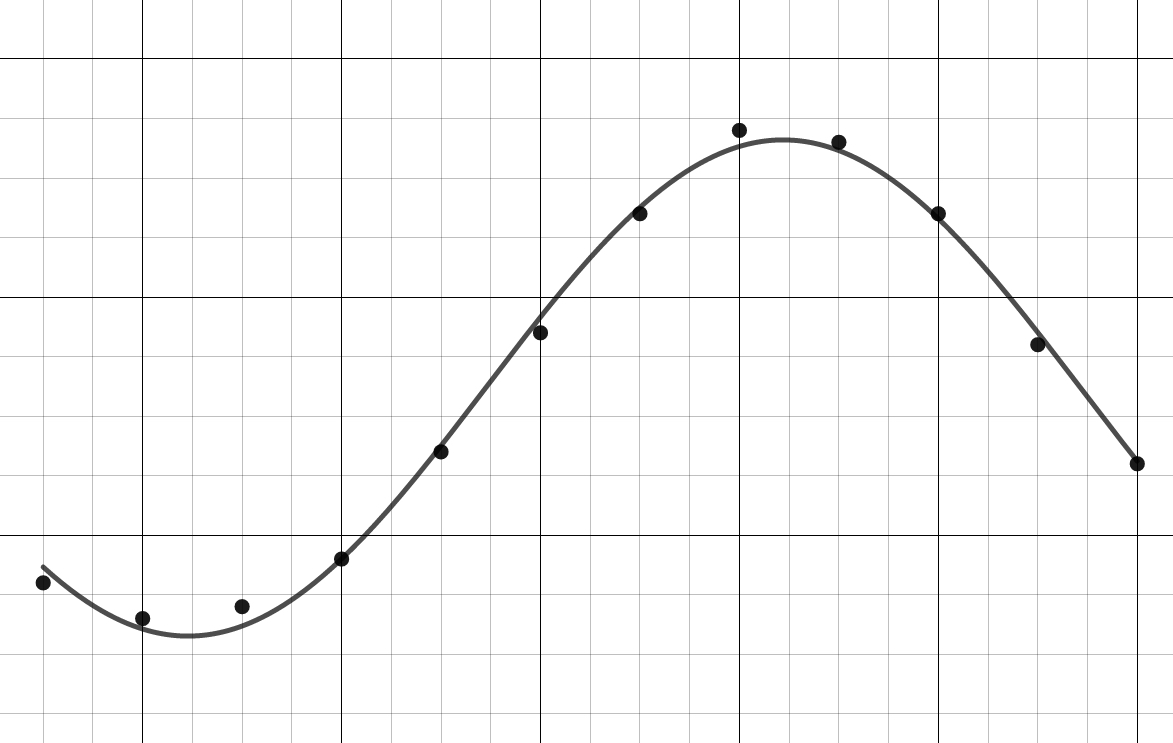
\includegraphics[height=1.5in]{./GraphsofSineandCosineGraphics/LakeErieRegDesmos.jpg} 

\end{center}

This model predicts the average temperature for April $15^{\text{th}}$ to be approximately $42.42^{\circ}$F and the average temperature on September $15^{\text{th}}$ to be approximately $70.05^{\circ}$F.  This model appears to be more accurate.

\end{enumerate}


\item  \begin{enumerate} \item  Based on the shape of the data, we either choose $A<0$ or we find the \textit{second} value of $t$ which closely approximates the `baseline' value, $F = 0.505$.  We choose the latter to obtain $F(t) = 0.475 \sin\left(\frac{\pi}{15} t - 2\pi \right) + 0.505 =  0.475 \sin\left(\frac{\pi}{15} t\right) + 0.505$ 

\enlargethispage{\baselineskip}

\item  Our function and the data set are graphed below.  It's a pretty good fit.

\begin{center}

 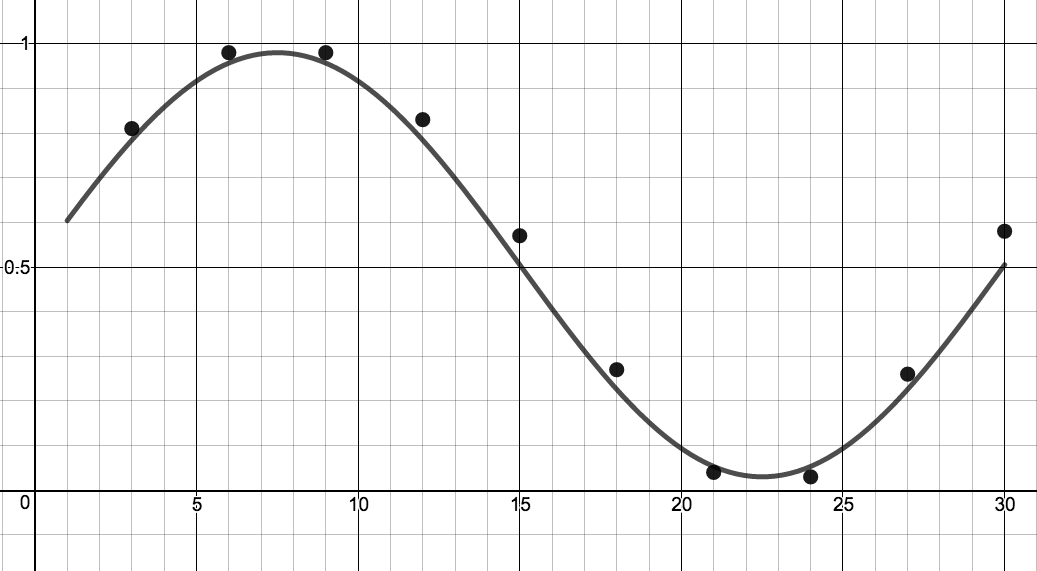
\includegraphics[height=1.5in]{./GraphsofSineandCosineGraphics/MoonIlluminationReg.jpg} 

\end{center}


\item  The fraction of the moon illuminated on June 1st, 2009 is approximately $F(1) \approx 0.60$


\item  Using desmos,\footnote{\ldots specifying $\omega = \frac{\pi}{15}$ \ldots} we get $F(t) = 0.49\sin \left(\frac{\pi }{15}t-6.29\right)+0.535$.

\begin{center}

 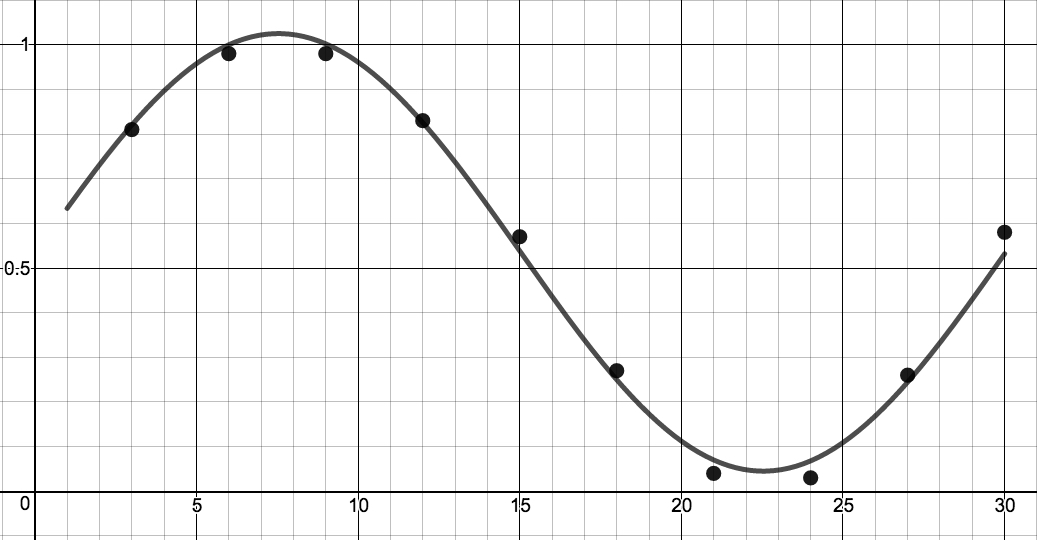
\includegraphics[height=1.5in]{./GraphsofSineandCosineGraphics/MoonIlluminatonDesmos.jpg} 

\end{center}

This model predicts that the fraction of the moon illuminated on June 1st, 2009 is approximately $0.63$.  This appears to be a better fit to the data than our first model.

\end{enumerate}


\end{enumerate}







\closegraphsfile

\newpage

\section{The Circular Functions: Tangent, Secant, Cosecant, and Cotangent}

\mfpicnumber{1}

\opengraphsfile{TheOtherCircularFunctions}

\setcounter{footnote}{0}

\label{TheOtherCircularFunctions}

In section \ref{TheCircularFunctionsSineandCosine},  we extended the notion of $\sin(\theta)$ and $\cos(\theta)$  from acute angles to any angles using the coordinate values of points on the Unit Circle. In total, there are six circular functions, as listed below.
\smallskip


\colorbox{ResultColor}{\bbm

\begin{defn} \label{circularfunctions}  \textbf{The Circular Functions:} Suppose an angle $\theta$ is graphed in standard position. 

\smallskip

Let $P(x,y)$ be the point of intersection of the terminal side of $P$ and the Unit Circle. 


 \begin{itemize}

\item The \index{sine ! of an angle} \textbf{sine} of $\theta$, denoted $\sin(\theta)$, is defined by $\sin(\theta) = y$. \vphantom{$\dfrac{y}{x}$}

\item The \index{cosine ! of an angle} \textbf{cosine} of $\theta$, denoted $\cos(\theta)$, is defined by $\cos(\theta) = x$. \vphantom{$\dfrac{y}{x}$}

\item The \index{tangent ! of an angle} \textbf{tangent} of $\theta$, denoted $\tan(\theta)$, is defined by $\tan(\theta) = \dfrac{y}{x}$, provided $x \neq 0$. \vphantom{$\dfrac{y}{x}$}

\item The \index{secant ! of an angle} \textbf{secant} of $\theta$, denoted $\sec(\theta)$, is defined by $\sec(\theta) = \dfrac{1}{x}$, provided $x \neq 0$. \vphantom{$\dfrac{y}{x}$}

\item The \index{cosecant ! of an angle} \textbf{cosecant} of $\theta$, denoted $\csc(\theta)$, is defined by $\csc(\theta) = \dfrac{1}{y}$, provided $y \neq 0$. \vphantom{$\dfrac{y}{x}$}

\item The \index{cotangent ! of an angle} \textbf{cotangent} of $\theta$, denoted $\cot(\theta)$, is defined by $\cot(\theta) = \dfrac{x}{y}$, provided $y \neq 0$. \vphantom{$\dfrac{y}{x}$}

\end{itemize}

\end{defn}

\smallskip

\ebm}

\smallskip

While we left the history of the name `sine' as an interesting research project in Section \ref{TheCircularFunctionsSineandCosine},we take a slight detour here to explain the origin of the names `tangent' and `secant.'  

\smallskip

Consider the acute angle $\theta$  in standard position sketched in the diagram below. 

\smallskip

\begin{center}

\begin{mfpic}[25]{-1}{7}{-1}{7}
\axes
\drawcolor[gray]{0.7}
\parafcn{0,90,5}{3*dir(t)}
\drawcolor{black}
\arrow \parafcn{5, 55, 5}{0.75*dir(t)}
\tlabel[cc](0.75,0.5){\scriptsize $\theta$}
\point[4pt]{(0,0), (1.5, 2.5981), (3,5.196), (3,0), (1.5,0)}
\tlabel(6.75,-0.5){\scriptsize $x$}
\tlabel(0.25,6.75){\scriptsize $y$}
\tlabel(0.25,3.1){\scriptsize $1$}
\tlabel(-0.5,-0.5){\scriptsize $O$}
\tlabel(2.75,-0.5){\scriptsize $B(1,0)$}
\tlabel(1.25, -0.5){\scriptsize $A(x, 0)$}
\xmarks{0 step 3 until 3}
\ymarks{0 step 3 until 3}
\polyline{(3,0), (3,5.196)}
\polyline{(2.75,0), (2.75, 0.25), (3,0.25)}
\polyline{(1.5,0), (1.5, 2.5981)}
\polyline{(1.25,0), (1.25,0.25), (1.5,0.25)}
\tlabel(1.75,2.6){\scriptsize $P(x,y)$}
\tlabel(3.25,5.25){\scriptsize $Q(1,y') = (1, \tan(\theta))$}
\penwd{1.25pt}
\arrow \reverse \arrow  \polyline{(7,0), (0,0), (4,6.9282)}
\end{mfpic} 

\end{center}

\smallskip

As usual, $P(x,y)$ denotes the point on the terminal side of $\theta$ which lies on the Unit Circle, but we also consider  the point $Q(1,y')$,  the point on the terminal side of $\theta$ which lies on the vertical line $x=1$. 

\smallskip

The word `tangent' comes from the Latin meaning `to touch,' and for this reason, the line $x=1$ is called a \textit{tangent} line to the Unit Circle since it intersects, or `touches', the circle at only one point, namely $(1,0)$.  

\smallskip

Dropping perpendiculars from $P$ and $Q$ creates a pair of similar triangles $\Delta OPA$ and $\Delta OQB$.  Hence the corresponding sides are proportional.  We get  $\frac{y'}{y} = \frac{1}{x}$ which gives  $y' = \frac{y}{x} = \tan(\theta)$.

\smallskip


 We have just shown that for acute angles $\theta$, $\tan(\theta)$ is the $y$-coordinate of the point on the terminal side of $\theta$ which lies on the line $x = 1$ which is \textit{tangent} to the Unit Circle. 
 
 \smallskip
 
 The word `secant' means `to cut', so a secant line is any line that `cuts through' a circle at two points.\footnote{Compare this with the definition given in Section \ref{AverageRateofChange}.}  The line containing the terminal side of $\theta$ (not just the terminal side itself) is one such secant line since it intersects the Unit Circle in Quadrants I and III.   
 
 \smallskip
 
 With the point $P$ lying on the Unit Circle, the length of the hypotenuse of $\Delta OPA$ is $1$. If we let $h$ denote the length of the hypotenuse of $\Delta OQB$, we have from similar triangles that $\frac{h}{1} = \frac{1}{x}$, or $h = \frac{1}{x} = \sec(\theta)$.  
 
 \smallskip
 
 Hence for an acute angle $\theta$, $\sec(\theta)$ is the length of the line segment which lies on the secant line determined by the terminal side of $\theta$ and `cuts off' the tangent line $x=1$.  
 
 \smallskip
 
As we mentioned in Definition \ref{sinecosineunitcircledefn}, the `co' in `cosecant' and `cotangent' tie back to the concept of `co'mplementary angles and is explained in detail in Section \ref{MoreTrigonometricIdentities}.

 \smallskip

 Not only do these observations help explain the names of these functions, they serve as the basis for a fundamental inequality needed for Calculus which we'll explore in the Exercises.

\smallskip 

Of the six circular functions, only sine and cosine are defined for all angles $\theta$.  Since $x = \cos(\theta) $ and $y = \sin(\theta) $ in Definition \ref{circularfunctions}, it is customary to rephrase the remaining four circular functions  Definition \ref{circularfunctions} in terms of sine and cosine.  


\smallskip

\colorbox{ResultColor}{\bbm

\begin{thm} \label{recipquotid}  \textbf{Reciprocal and Quotient Identities:} \index{Reciprocal Identities} \index{Quotient Identities} 

\begin{itemize}

\item $\sec(\theta) = \dfrac{1}{\cos(\theta)}$, provided $\cos(\theta) \neq 0$;  if $\cos(\theta) = 0$, $\sec(\theta)$ is undefined.

\item $\csc(\theta) = \dfrac{1}{\sin(\theta)}$, provided $\sin(\theta) \neq 0$;  if $\sin(\theta) = 0$, $\csc(\theta)$ is undefined.

\item $\tan(\theta) = \dfrac{\sin(\theta)}{\cos(\theta)}$, provided $\cos(\theta) \neq 0$;  if $\cos(\theta) = 0$, $\tan(\theta)$ is undefined.

\item $\cot(\theta) = \dfrac{\cos(\theta)}{\sin(\theta)}$, provided $\sin(\theta) \neq 0$;  if $\sin(\theta) = 0$, $\cot(\theta)$ is undefined.

\end{itemize}

\end{thm}

\ebm}

\smallskip

We call the equations listed in Theorem \ref{recipquotid}  \index{identity ! equation}\index{equation ! identity}\textbf{identities} since they are relationships which are true regardless of the values of $\theta$.  This is in contrast to \index{conditional equation}\index{equation ! conditional}\textbf{conditional equations} such as $\sin(\theta) = 1$ which are true for only \textbf{some} values of $\theta$.  We will study identities more extensively in Sections \ref{FundamentalTrigonometricIdentities} and \ref{MoreTrigonometricIdentities}.

\smallskip

While the Reciprocal and Quotient Identities presented in Theorem \ref{recipquotid} allow us to always reduce problems involving secant, cosecant, tangent and cotangent to problems involving sine and cosine, it is not always convenient to do so.\footnote{As we shall see shortly, when solving equations involving secant and cosecant, we usually convert back to cosines and sines.  However, when solving for tangent or cotangent, we usually stick with what we're dealt.}  It is worth taking the time to memorize the tangent and cotangent values of the common angles summarized below.

\smallskip

\begin{center}

\textbf{Tangent and Cotangent Values of Common Angles}

\vspace{-.25in}

\setlength{\extrarowheight}{4pt}

\[ \begin{array}{|c|c||c|c|} \hline
 \theta (\mbox{degrees}) &  \theta (\mbox{radians}) & \tan(\theta) & \cot(\theta) \\ \hline
0^{\circ} & 0 & 0 & \text{undefined} \\ \hline
30^{\circ} & \frac{\pi}{6} & \frac{\sqrt{3}}{3} & \sqrt{3} \\ [2pt] \hline
45^{\circ} & \frac{\pi}{4} & 1 & 1 \\ [2pt] \hline
60^{\circ} & \frac{\pi}{3} & \sqrt{3} & \frac{\sqrt{3}}{3} \\ [2pt] \hline
90^{\circ} & \frac{\pi}{2} & \text{undefined} & 0 \\ [2pt] \hline
\end{array} \]

\setlength{\extrarowheight}{2pt}

\end{center}

Coupling Theorem \ref{recipquotid} with the Reference Angle Theorem, Theorem \ref{refanglethm}, we get the following.

\smallskip

\colorbox{ResultColor}{\bbm

\begin{thm} \label{genrefanglethm} \textbf{Generalized Reference Angle Theorem.}  The values of the circular functions of an angle, if they exist, are the same, up to a sign, of the corresponding circular functions of its reference angle. 

\smallskip

More specifically, if $\alpha$ is the reference angle for $\theta$,  then: 

\smallskip

  \centerline{$\sin(\theta) = \pm \sin(\alpha)$,  $\cos(\theta) = \pm \cos(\alpha)$,  $\tan(\theta) = \pm \tan(\alpha)$}
  
  \centerline{and}
  
    \centerline{$\sec(\theta) = \pm \sec(\alpha)$,  $\csc(\theta) = \pm \csc(\alpha)$,  $\cot(\theta) = \pm \cot(\alpha)$}
    
    \smallskip


where the choice of the ($\pm$) depends on the quadrant in which the terminal side of $\theta$ lies.\index{Reference Angle Theorem ! for the circular functions}

\end{thm}

\ebm}

\smallskip

It is high time for an example.


\begin{ex} \label{circularfunctionsex}  $~$

\begin{enumerate}

\item  Find the exact value of the following, if it exists:

\begin{multicols}{4}

\begin{enumerate}

\item  $\sec\left(60^{\circ}\right)$

\item  $\csc\left(\frac{7 \pi}{4} \right)$

\item  $\tan(225^{\circ})$

\item  $\cot\left(-\frac{7 \pi}{6} \right)$

\end{enumerate}

\end{multicols}

\item Find all angles which satisfy the given equation.   

\begin{multicols}{4}

\begin{enumerate}

\item  $\sec(\theta) =2$

\item  $\csc(\theta) = -\sqrt{2}$

\item  $\tan(\theta) = \sqrt{3}$

\item  \label{cotangentisnegativeone} $\cot(\theta) = -1$.

\end{enumerate}

\end{multicols}

\end{enumerate}

{\bf Solution.}  

\begin{enumerate}

\item \begin{enumerate}

\item  According to Theorem \ref{recipquotid},   $\sec\left(60^{\circ}\right) = \frac{1}{\cos\left(60^{\circ}\right)}$. Hence,  $\sec\left(60^{\circ}\right) = \frac{1}{(1/2)} = 2$.

\item  Since $\sin\left( \frac{7\pi}{4}\right) = - \frac{\sqrt{2}}{2}$,  $\csc\left( \frac{7\pi}{4}\right) = \frac{1}{\sin\left( \frac{7\pi}{4}\right)} = \frac{1}{- \sqrt{2}/2} = - \frac{2}{\sqrt{2}} = - \sqrt{2}$.

\item  We have two ways to proceed to determine  $\tan(225^{\circ})$.  First, we can use Theorem \ref{recipquotid} and note that $\tan(225^{\circ})  = \frac{\sin(225^{\circ})}{\cos(225^{\circ})}$.  Since $\sin(225^{\circ}) = \cos(225^{\circ}) = -\frac{\sqrt{2}}{2}$, $\tan(225^{\circ}) = 1$.

\smallskip

Another way to proceed is to note that $225^{\circ}$ has a reference angle of $45^{\circ}$.   Per Theorem \ref{genrefanglethm},  $\tan(225^{\circ}) = \pm \tan(45^{\circ}) = \pm 1$.  Since  $225^{\circ}$ is a Quadrant III angle, where both the $x$ and $y$ coordinates of points are both negative, and tangent is defined as the \textit{ratio} of coordinates $\frac{y}{x}$, we know $\tan(225^{\circ}) > 0$.  Hence,  $\tan(225^{\circ}) = 1$.

\item  As with the previous example, we have two ways to proceed.  Using Theorem \ref{recipquotid}, we have $\cot\left(-\frac{7 \pi}{6} \right) = \frac{\cos\left(-\frac{7 \pi}{6} \right)}{\sin\left(-\frac{7 \pi}{6} \right)}$.  Since $\cos\left(-\frac{7 \pi}{6} \right) = -\frac{\sqrt{3}}{2}$ and $\sin\left(-\frac{7 \pi}{6} \right) = \frac{1}{2}$, we get  $\cot\left(-\frac{7 \pi}{6} \right) = - \sqrt{3}$.

\smallskip

Alternatively, we note $-\frac{7 \pi}{6}$ is a Quadrant II angle with reference angle $\frac{\pi}{6}$.  Hence, Theorem \ref{genrefanglethm} tells us $\cot\left(-\frac{7 \pi}{6} \right) = \pm \cot\left(\frac{\pi}{6} \right) = \pm \sqrt{3}$.  Since $-\frac{7 \pi}{6}$ is a Quadrant II angle, where the $x$ and $y$ coordinates have different signs, and cotangent is defined as the ratio of coordinates $\frac{x}{y}$, we know $\cot\left(-\frac{7 \pi}{6} \right)<0$.  Hence, $\cot\left(-\frac{7 \pi}{6} \right) = -\sqrt{3}$.

\end{enumerate}

\item  \begin{enumerate}

\item  To solve $\sec(\theta) = 2$, we convert to cosines and get $\frac{1}{\cos(\theta)} = 2$ or $\cos(\theta) = \frac{1}{2}$.  This is the exact same equation we solved in Example \ref{solveforangle}, number \ref{cosineishalf}, so we know the answer is:  $\theta = \frac{\pi}{3} + 2\pi k$ or $\theta = \frac{5\pi}{3} + 2\pi k$ for integers $k$.

\item From the table of common values, we see  $\tan\left(\frac{\pi}{3}\right) = \sqrt{3}$.  According to Theorem \ref{genrefanglethm}, we  know  the solutions to $\tan(\theta) = \sqrt{3}$ must, therefore, have a reference angle of $\frac{\pi}{3}$. 

\smallskip

To find the quadrants in which our solutions lie, we note that tangent is defined as the ratio $\frac{y}{x}$ of points $(x,y)$ on the Unit Circle.  Hence, tangent is positive when $x$ and $y$ have the same sign (i.e., when they are both positive or both negative.) This happens in Quadrants I and III. 

\smallskip

 In Quadrant I, we get the solutions: $\theta = \frac{\pi}{3} + 2\pi k$ for integers $k$, and for Quadrant III, we get $\theta = \frac{4\pi}{3} + 2\pi k$ for integers $k$.  While these descriptions of the solutions are correct, they can be combined into one list as $\theta = \frac{\pi}{3} + \pi k$ for integers $k$. The latter form of the solution is best understood looking at the geometry of the situation in the diagram below.\footnote{See Example \ref{solveforangle} number \ref{cosineiszero} in Section \ref{TheCircularFunctionsSineandCosine} for another example of this kind of simplification of the solution.}
 

\begin{tabular}{cc}

\begin{mfpic}[15]{-5.25}{5.25}{-5.25}{5.5}
\axes
\tlabel(5.25,-0.5){\scriptsize $x$}
\tlabel(0.25,5.25){\scriptsize $y$}
\tlabel(4.6,-1){\scriptsize $1$}
\tlabel(0.25,4.6){\scriptsize $1$}
\xmarks{-4.5, 4.5}
\ymarks{-4.5 step 4.5 until 4.5}
\drawcolor[gray]{0.7}
\circle{(0,0),4.5}
\drawcolor{black}
\arrow \reverse \arrow \parafcn{5, 55, 5}{1.5*dir(t)}
\tlabel(1.5, 1){$\frac{\pi}{3}$}
\point[4pt]{(0,0), (2.25, 3.8971)}
\penwd{1.25pt}
\arrow \polyline{(5.25, 0), (0,0), (2.5, 4.330)}
\end{mfpic} 

&

\hspace{.75in}

\begin{mfpic}[15]{-5.25}{5.25}{-5.25}{5.5}
\axes
\tlabel(5.25,-0.5){\scriptsize $x$}
\tlabel(0.25,5.25){\scriptsize $y$}
\tlabel(4.6,-1){\scriptsize $1$}
\tlabel(0.25,4.6){\scriptsize $1$}
\xmarks{-4.5, 4.5}
\ymarks{-4.5 step 4.5 until 4.5}
\drawcolor[gray]{0.7}
\circle{(0,0),4.5}
\drawcolor{black}

\arrow \reverse \arrow \parafcn{185, 235, 5}{2*dir(t)}
\tlabel(-2.6, -1.5){$\frac{\pi}{3}$}
\point[4pt]{(0,0), (-2.25, -3.8971)}
\arrow \dashed \polyline{(0,0), (2.5, 4.330)}
\arrow \reverse \arrow \parafcn{5, 55, 5}{1.5*dir(t)}
\tlabel(1.5, 1){$\frac{\pi}{3}$}
\tlabel(-1.5, 2){$\pi$}
\point[4pt]{(2.25, 3.8971)}
\arrow \reverse \arrow \parafcn{65, 235, 5}{1.5*dir(t)}
\penwd{1.25pt}
\arrow \polyline{(5.25, 0), (0,0), (-2.5, -4.330)}
\end{mfpic} 
\end{tabular}
  

\item  From the table of common values, we see that $\frac{\pi}{4}$ has a cotangent of $1$, which means the solutions to $\cot(\theta) = -1$ have a reference angle of $\frac{\pi}{4}$. 

\smallskip

To find the quadrants in which our solutions lie, we note that $\cot(\theta) = \frac{x}{y}$ for a point $(x,y)$ on the Unit Circle where $y \neq 0$. If $\cot(\theta)$ is negative, then $x$ and $y$ must have different signs (i.e., one positive and one negative.)  Hence, our solutions lie in Quadrants II and IV.  

\smallskip

Our Quadrant II solution is $\theta = \frac{3\pi}{4} + 2\pi k$, and for Quadrant IV, we get $\theta = \frac{7\pi}{4} + 2\pi k$ for integers $k$.  As in the previous problem, we can combine these solutions as:  $\theta = \frac{3\pi}{4} + \pi k$ for integers $k$.


\begin{tabular}{cc}

\begin{mfpic}[15]{-5.25}{5.25}{-5.25}{5.5}
\axes
\tlabel(5.25,-0.5){\scriptsize $x$}
\tlabel(0.25,5.25){\scriptsize $y$}
\tlabel(4.6,-1){\scriptsize $1$}
\tlabel(0.25,4.6){\scriptsize $1$}
\xmarks{-4.5, 4.5}
\ymarks{-4.5 step 4.5 until 4.5}
\drawcolor[gray]{0.7}
\circle{(0,0),4.5}
\drawcolor{black}
\arrow \reverse \arrow \parafcn{140, 175, 5}{1.5*dir(t)}
\tlabel[cc](-2, 1){$\frac{\pi}{4}$}
\point[4pt]{(0,0), (-3.1820, 3.1820)}
\penwd{1.25pt}
\arrow \polyline{(5.25,0), (0,0), (-3.5355, 3.5355)}
\end{mfpic} 

&

\hspace{.75in}

\begin{mfpic}[15]{-5.25}{5.25}{-5.25}{5.5}
\axes
\tlabel(5.25,-0.5){\scriptsize $x$}
\tlabel(0.25,5.25){\scriptsize $y$}
\tlabel(4.6,-1){\scriptsize $1$}
\tlabel(0.25,4.6){\scriptsize $1$}
\xmarks{-4.5, 4.5}
\ymarks{-4.5 step 4.5 until 4.5}
\drawcolor[gray]{0.7}
\circle{(0,0),4.5}
\drawcolor{black}
\arrow \reverse \arrow \parafcn{320, 355, 5}{1.5*dir(t)}
\tlabel[cc](2, -1){$\frac{\pi}{4}$}
\tlabel[cc](-1.77, -1.77){$\pi$}
\point[4pt]{(0,0), (3.1820, -3.1820), (-3.1820, 3.1820)}
\arrow \dashed \polyline{(0,0), (-3.5355, 3.5355)}
\arrow \reverse \arrow \parafcn{140, 175, 5}{2*dir(t)}
\arrow \reverse \arrow \parafcn{140, 310, 5}{1.5*dir(t)}
\tlabel[cc](-2.31, 0.96){$\frac{\pi}{4}$}
\penwd{1.25pt}
\arrow \polyline{(5.25,0), (0,0), (3.5355, -3.5355)}
\end{mfpic}
\end{tabular}

\end{enumerate}
\end{enumerate}

\vspace{-.3in} \qed

\end{ex}

A few remarks about Example \ref{circularfunctionsex} are in order.  First note that the signs ($\pm$) of secant and cosecant are the same as the signs of cosine and sine, respectively.  

\smallskip

On the other hand, since tangent and cotangent are defined in terms of the \textit{ratios} of coordinates $x$ and $y$, tangent and cotangent are positive in Quadrants I and III (where both $x$ and $y$ have the same sign) and negative in Quadrants II and IV (where $x$ and $y$ have opposite signs.)  

\smallskip
 
 The diagram below on the left summarizes which circular functions are positive in which quadrants.
 
 \smallskip
 
 \begin{multicols}{2}
 
\begin{mfpic}[18]{-4}{5}{-5}{5}
\axes
\tlabel(4.75,-0.5){\scriptsize $x$}
\tlabel(0.25,5){\scriptsize $y$}
\tlabel(3.1,-0.75){\scriptsize $(1,0)$}
\tlabel(-4.5,-0.75){\scriptsize $(-1,0)$}
\tlabel(0.25,3.1){ \scriptsize $(0,1)$}
\tlabel(0.25,-3.4){\scriptsize $(0,-1)$}
\tlabel[cc](1,0.75){\scriptsize All}
\tlabel[cc](-1.5,0.75){\scriptsize $\sin(\theta)$, $\csc(\theta)$}
\tlabel[cc](-1.5,-0.75){\scriptsize $\tan(\theta)$, $\cot(\theta)$}
\tlabel[cc](1.5,-0.75){\scriptsize $\cos(\theta)$, $\sec(\theta)$}
\tcaption{Postive Circular Functions}
\tlabel[cc](-2.83,-2.83){$(-,-)$}
\tlabel[cc](2.83,2.83){$(+, +)$}
\tlabel[cc](-2.83,2.83){$(-,+)$}
\tlabel[cc](2.83,-2.83){$(+,-)$}
\xmarks{-3 step 3 until 3}
\ymarks{-3 step 3 until 3}
\drawcolor[gray]{0.7}
\circle{(0,0),3}
\point[4pt]{(-2.1213, -2.1213),(2.1213, 2.1213), (2.1213, -2.1213),(-2.1213, 2.1213), (0,3), (3,0), (0,-3), (-3,0) }
\end{mfpic} 

\begin{mfpic}[18]{-4}{5}{-5}{5}
\axes
\tlabel(4.75,-0.5){\scriptsize $x$}
\tlabel(0.25,5){\scriptsize $y$}
\tlabel(3.1,-0.75){\scriptsize $(1,0)$}
\tlabel(-4.5,-0.75){\scriptsize $(-1,0)$}
\tlabel(0.25,3.1){ \scriptsize $(0,1)$}
\tlabel(0.25,-3.4){\scriptsize $(0,-1)$}
\tcaption{The period of $\tan(\theta)$ and $\cot(\theta)$ is $\pi$}
\dashed \polyline{(-2.25, -3.9), (2.25, 3.9)}
\arrow \reverse \arrow \parafcn{65, 235, 5}{2.25*dir(t)}
\arrow \reverse \arrow \parafcn{245, 415, 5}{2.25*dir(t)}
\arrow \reverse \arrow \parafcn{5, 55, 5}{1.25*dir(t)}
\arrow \reverse \arrow \parafcn{185, 235, 5}{1.25*dir(t)}
\tlabel[cc](-1.8, 1.8){$\pi$}
\tlabel[cc](1.8, -1.8){$\pi$}
\xmarks{-3 step 3 until 3}
\ymarks{-3 step 3 until 3}
\drawcolor[gray]{0.7}
\circle{(0,0),3}
\point[4pt]{(-1.5, -2.6),(1.5, 2.6) }
\end{mfpic} 


\end{multicols}

Also note it is no coincidence that both of our solutions to the equations involving tangent and cotangent in  Example \ref{circularfunctionsex} could be simplified to just one list of angles differing by multiples of $\pi$.  

\smallskip

Indeed, any two angles that are $\pi$ units apart will not only have the same reference angle, but points on their terminal sides on the Unit Circle will be reflections through the origin, as illustrated above on the right.

\smallskip

It follows that the tangent and cotangent of such angles (if defined) will be the same, which means the period of these function is (at most) $\pi$.  

\smallskip

Using an argument similar to the one we used to establish the period of sine and cosine in Section \ref{GraphsofSineandCosine}, we note that if $\tan(x+p) = \tan(x)$ for all real numbers $x$, then, in particular,   $\tan(p) = \tan(0+p) = \tan(0) = 0$.  Hence,  $p$ is a multiple of $\pi$, and the smallest multiple of $\pi$ is $\pi$ itself.  

\smallskip

Hence, the period of tangent (and cotangent) is $\pi$, and we will see the consequences of this both when solving equations in this section and when graphing these functions in Section \ref{GraphsofOtherCircularFunctions}.

\smallskip  

As with sine and cosine, the circular functions defined in Definition \ref{circularfunctions}  agree with those put forth in Definitions \ref{righttrianglesinecosinetangent} and \ref{righttriangletherest} in Section \ref{AppRightTrig} for acute angles situated in right triangles.  The argument is identical to the one given in Section \ref{TheCircularFunctionsSineandCosine} and is left to the reader.  

\smallskip

Moreover,  Definition \ref{circularfunctions}  can be extended to circles of arbitrary radius $r>0$ using the same similarity arguments in Section \ref{cosinesinebeyond} to generalize Definition \ref{sinecosineunitcircledefn} to Theorem \ref{cosinesinecircle} as summarized below.

\smallskip

\colorbox{ResultColor}{\bbm

\begin{thm} \label{circularfunctionscircle} Suppose $Q(x,y)$ is the point on the terminal side of an angle $\theta$ (plotted in standard position) which lies on the circle of radius $r$,  $x^2+y^2 = r^2$. Then:

\begin{itemize}

\item  $\sin(\theta) = \dfrac{y}{r} = \dfrac{y}{\sqrt{x^2+y^2}}$ \index{sine ! of an angle}

\item $\cos(\theta)= \dfrac{x}{r}  = \dfrac{x}{\sqrt{x^2+y^2}}$ \index{cosine ! of an angle}

\item $\tan(\theta) = \dfrac{y}{x}$, provided $x \neq 0$. \index{tangent ! of an angle}

\item $\sec(\theta) = \dfrac{r}{x} = \dfrac{\sqrt{x^2+y^2}}{x}$, provided $x \neq 0$. \index{secant ! of an angle}

\item $\csc(\theta) = \dfrac{r}{y} = \dfrac{\sqrt{x^2+y^2}}{y}$, provided $y \neq 0$. \index{cosecant ! of an angle}

\item $\cot(\theta) = \dfrac{x}{y}$, provided $y \neq 0$. \index{cotangent ! of an angle}

\end{itemize}

\end{thm}

\ebm}

\smallskip

We make good use of Theorem \ref{circularfunctionscircle}  in the following example.

\begin{ex} \label{circularfunctionscircleex}  Use Theorem \ref{circularfunctionscircle} to solve the following.

\begin{enumerate}

\item  Suppose the terminal side of $\theta$, when plotted in standard position, contains the point $Q(3,4)$.  Find the values of the six circular functions of $\theta$.

\item  Suppose $\theta$ is a Quadrant IV angle with $\cot(\theta) = -4$.  Find the values of the five remaining circular functions of $\theta$.

\item Find $\sin\left(\theta\right)$, where $\sec(\theta) = -\sqrt{5}$ and $\theta$ is a Quadrant II angle.

\item \label{commontanmistake} Find $\cos\left(\theta\right)$, where $\tan(\theta) = 3$ and $\pi < \theta < \frac{3\pi}{2}$.

\end{enumerate}

{\bf Solution.}

\begin{enumerate}

\item    Since $x = 3$ and $y=4$, from $x^2+y^2 = r^2$, $(3)^2+(4)^2 = r^2$ so $r^2 = 25$, or $r = 5$. Theorem \ref{circularfunctionscircle} tells us $\sin(\theta) = \frac{4}{5}$, $\cos(\theta) = \frac{3}{5}$,  $\tan(\theta) = \frac{4}{3}$, $\sec(\theta) = \frac{5}{3}$, $\csc(\theta) = \frac{5}{4}$,  and $\cot(\theta) = \frac{3}{4}$.

\item In order to use Theorem \ref{circularfunctionscircle}, we need to find a point $Q(x,y)$ which lies on the terminal side of $\theta$, when $\theta$ is plotted in standard position.  


\smallskip

We have that $\cot(\theta) = -4 =  \frac{x}{y}$.  Since  $\theta$ is a Quadrant IV angle, we also know $x>0$ and $y< 0$.  Rewriting   $-4 = \frac{4}{-1}$, we choose\footnote{We could have just as easily chosen $x=8$ and $y=-2$ - just so long as $x>0$, $y<0$ and $\frac{x}{y} = -4$.}   $x = 4$ and $y = -1$ so that $r = \sqrt{x^2+y^2} = \sqrt{(4)^2 + (-1)^2} = \sqrt{17}$.  

\smallskip

Applying Theorem \ref{circularfunctionscircle}, we find  $\sin(\theta) =- \frac{1}{\sqrt{17}} = -\frac{\sqrt{17}}{17}$, $\cos(\theta) = \frac{4}{\sqrt{17}} = \frac{4 \sqrt{17}}{17}$,  $\tan(\theta) = -\frac{1}{4}$, $\sec(\theta) = \frac{\sqrt{17}}{4}$, and $\csc(\theta) = - \sqrt{17}$.

\begin{tabular}{cc}

\begin{mfpic}[18]{-5}{5}{-4}{4.75}
\axes
\tlabel(4.75,-0.5){\scriptsize $x$}
\tlabel(0.25,4.5){\scriptsize $y$}
\tlabel(2.75,3){\scriptsize $Q(3,4)$}
\tlabel[cc](2,1.5){\scriptsize $r=5$}
\tcaption{$Q(3,4)$ lies on a circle of radius $5$ units,}
\xmarks{-2.68, -2,  -1.34, -0.67, 0.67, 1.34, 2, 2.68}
\ymarks{-2.68, -2,  -1.34, -0.67, 0.67, 1.34, 2, 2.68}
\drawcolor[gray]{0.7}
\circle{(0,0),3.354}
\drawcolor{black}
\penwd{1.25pt}
\arrow \reverse \arrow \polyline{(5,0),(0,0), (3, 4)}
\point[4pt]{(0,0), (2.012, 2.683)}
\tlpointsep{4pt}
\scriptsize 
\axislabels {x}{ {$-3 \hspace{7pt}$} -2, {$-1 \hspace{7pt}$} -0.67,  {$1$} 0.67,  {$3$} 2, {$-2 \hspace{7pt}$} -1.34, {$-4 \hspace{7pt}$} -2.68, {$2$} 1.34, {$4$} 2.68}
\axislabels {y}{ {$-2$} -1.34, {$-4$} -2.68, {$2$} 1.34, {$4$} 2.68,  {$1$} 0.67,  {$3$} 2,  {$-1$} -0.67,  {$-3$} -2 }
\normalsize
\end{mfpic}

&

\begin{mfpic}[18]{-5}{5}{-4}{4.75}
\axes
\tlabel(4.75,-0.5){\scriptsize $x$}
\tlabel(0.25,4.5){\scriptsize $y$}
\tlabel[cc](1.4, -1.25){\scriptsize $r = \sqrt{17}$}
\tlabel[cc](4, -1.5){\scriptsize $(4, -1)$}
\tcaption{$\theta$ is Quadrant IV with $\cot(\theta) = -4$.}
\xmarks{-3.24, -1.62, 1.62, 3.24, 0.81, -0.81, 2.43, -2.43}
\ymarks{-3.24, -1.62, 1.62, 3.24, 0.81, -0.81, 2.43, -2.43}
\drawcolor[gray]{0.7}
\circle{(0,0),3.354}
\drawcolor{black}
\penwd{1.25pt}
\arrow \reverse \arrow \polyline{(5,0),(0,0), (4.92, -1.23)}
\point[4pt]{(0,0), (3.24, -0.81)}
\tlpointsep{4pt}
\scriptsize 
\axislabels {x}{ {$4$} 3.24, {$3$} 2.43, {$-4 \hspace{7pt}$} -3.24, {$-2$ \hspace{7pt}} -1.62, {$-1 \hspace{7pt}$} -0.81, {$-3 \hspace{7pt}$} -2.43}
\axislabels {y}{ {$4$} 3.24, {$2$} 1.62, {$1$} 0.81, {$3$} 2.43, {$-4$} -3.24, {$-2$} -1.62, {$-1$} -0.81, {$-3$} -2.43}
\normalsize
\end{mfpic}


\end{tabular}


\item To find $\sin(\theta)$ using Theorem \ref{circularfunctionscircle}, we need to determine the $y$-coordinate of a point $Q(x,y)$ on the terminal side of $\theta$, when $\theta$ is plotted in standard position,  and the corresponding radius $r$. 

\smallskip

Since   $\sec(\theta) = \frac{r}{x}$ and $r > 0$, we rewrite  $\sec(\theta) = \frac{r}{x}  = -\sqrt{5} = \frac{\sqrt{5}}{-1}$ and take $r = \sqrt{5}$ and $x = -1$.

\smallskip

To find $y$, we substitute $x=-1$ and $r=\sqrt{5}$ into $x^2+y^2 = r^2$ to get $(-1)^2+y^2=(\sqrt{5})^2$.  We find $y^2 = 4$ or $y = \pm 2$.   Since $\theta$ is a Quadrant II angle, we select $y = 2$.

\smallskip

Hence, $\sin(\theta) = \frac{y}{r} = \frac{2}{\sqrt{5}} = \frac{2 \sqrt{5}}{5}$.


\item  We are told $\tan(\theta) = 3$ and  $\pi < \theta < \frac{3\pi}{2}$, so we know $\theta$ is a Quadrant III angle. 

\smallskip

 To find $\cos(\theta)$ using Theorem \ref{circularfunctionscircle},  we need to find the $x$-coordinate of a point $Q(x,y)$ on the terminal side of $\theta$, when $\theta$ is plotted in standard position,  and the corresponding radius, $r$.

\smallskip

Since $\tan(\theta) = \frac{y}{x}$ and $\theta$ is a Quadrant III angle, we rewrite $\tan(\theta) = 3 = \frac{-3}{-1}  = \frac{y}{x}$ and choose $x = -1$ and $y = -3$.  From $x^2+y^2 = r^2$, we get $r = \sqrt{10}$.

\smallskip

Hence, $\cos(\theta) = \frac{x}{r} = \frac{-1}{\sqrt{10}} = -\frac{\sqrt{10}}{10}$.

\begin{tabular}{cc}

\begin{mfpic}[18]{-5}{5}{-4}{4.75}
\axes
\tlabel(4.75,-0.5){\scriptsize $x$}
\tlabel(0.25,4.5){\scriptsize $y$}
\tlabel[cc](-3, 3){\scriptsize $Q(-2, 1)$}
\tlabel[cc](-1.75,1.5){\scriptsize $r=\sqrt{5}$}
\tcaption{$\theta$ is Quadrant II with $\sec(\theta) = -\sqrt{5}$}
\xmarks{-1.5, -3, -4.5, 1.5, 3, 4.5}
\ymarks{-1.5, -3,1.5, 3, 4.5}
\drawcolor[gray]{0.7}
\circle{(0,0),3.354}
\drawcolor{black}
\penwd{1.25pt}
\arrow \reverse \arrow \polyline{(5,0),(0,0), (-2.25, 4.5)}
\point[4pt]{(0,0), (-1.5,3)}
\tlpointsep{4pt}
\scriptsize 
\axislabels {x}{ {$-1 \hspace{7pt}$} -1.5, {$-2 \hspace{7pt}$} -3, {$-3 \hspace{7pt}$} -4.5, {$1$} 1.5, {$2$} 3, {$3$} 4.5}
\axislabels {y}{ {$-2$} -3, {$-1$} -1.5, {$1$} 1.5, {$2$} 3}
\normalsize
\end{mfpic}

&

\begin{mfpic}[18]{-5}{5}{-4}{4.75}
\axes
\tlabel(4.75,-0.5){\scriptsize $x$}
\tlabel(0.25,4.5){\scriptsize $y$}
\tlabel[cc](-2, -1.25){\scriptsize $r = \sqrt{10}$}
\tlabel[cc](-2.5, -3.18){\scriptsize $(-1, -3)$}
\tcaption{$\theta$ is Quadrant III with $\tan(\theta) = 3$.}
\xmarks{1.06, 2.12, 3.18, 4.24, -1.06, -2.12, -3.18, -4.24 }
\ymarks{1.06, 2.12, 3.18, -1.06, -2.12, -3.18 }
\drawcolor[gray]{0.7}
\circle{(0,0),3.354}
\drawcolor{black}
\penwd{1.25pt}
\arrow \reverse \arrow \polyline{(5,0),(0,0), (-1.58, -4.74)}
\point[4pt]{(0,0), (-1.06, -3.18)}
\tlpointsep{4pt}
\scriptsize 
\axislabels {x}{  {$4$} 4.24, {$3$} 3.18, {$2$} 2.12,  {$1$} 1.06, {$-4 \hspace{7pt}$} -4.24, {$-3 \hspace{7pt}$} -3.18, {$-2 \hspace{7pt}$} -2.12,  {$-1 \hspace{7pt}$} -1.06}
\axislabels {y}{ {$3$} 3.18, {$2$} 2.12,  {$1$} 1.06, {$-3$} -3.18, {$-2$} -2.12}
\normalsize
\end{mfpic}


\end{tabular}


\qed


\end{enumerate}

\end{ex}



As we did in Section \ref{cosinesinebeyond}, we may consider $\tan(t)$, $\sec(t)$, $\csc(t)$, and $\cot(t)$ as functions \textit{real numbers} by associating each real number $t$ with an angle $\theta$ measuring $t$ radians as discussed on page \pageref{cosinesineequationsrealnumbers} and using Definition \ref{circularfunctions}, or, more generally, Theorem \ref{circularfunctionscircle}.
\smallskip

Alternatively, we could define each of these four functions in terms of $f(t) = \sin(t)$ and $g(t) = \cos(t)$ as demonstrated in Theorem \ref{recipquotid}.  For example, we could simply \textit{define} $\sec(t) = \frac{1}{\cos(t)}$ so long as $\cos(t) \neq 0$.  

\smallskip

Either way, we have the means to explore these functions in  greater  detail.  Before doing so, we'll need practice with these additional four circular functions courtesy of the Exercises.


\newpage

\subsection{Exercises}

In Exercises \ref{circvaluefirst} - \ref{circvaluelast}, find the exact value or state that it is undefined.

\begin{multicols}{4}

\begin{enumerate}

\item $\tan \left( \dfrac{\pi}{4} \right)$ \vphantom{$\csc \left( \dfrac{5\pi}{6} \right)$} \label{circvaluefirst}
\item $\sec \left( \dfrac{\pi}{6} \right)$ \vphantom{$\csc \left( \dfrac{5\pi}{6} \right)$}
\item $\csc \left( \dfrac{5\pi}{6} \right)$
\item $\cot \left( \dfrac{4\pi}{3} \right)$

\setcounter{HW}{\value{enumi}}

\end{enumerate}

\end{multicols}

\begin{multicols}{4}

\begin{enumerate}

\setcounter{enumi}{\value{HW}}

\item $\tan \left( -\dfrac{11\pi}{6} \right)$
\item $\sec \left( -\dfrac{3\pi}{2} \right)$
\item $\csc \left( -\dfrac{\pi}{3} \right)$ \vphantom{$\csc \left( \dfrac{5\pi}{6} \right)$}
\item $\cot \left( \dfrac{13\pi}{2} \right)$

\setcounter{HW}{\value{enumi}}

\end{enumerate}

\end{multicols}

\begin{multicols}{4}

\begin{enumerate}

\setcounter{enumi}{\value{HW}}

\item $\tan \left( 117\pi \right)$ \vphantom{$\csc \left( \dfrac{5\pi}{6} \right)$}
\item $\sec \left( -\dfrac{5\pi}{3} \right)$
\item $\csc \left( 3\pi \right)$ \vphantom{$\csc \left( \dfrac{5\pi}{6} \right)$}
\item $\cot \left( -5\pi \right)$ \vphantom{$\csc \left( \dfrac{5\pi}{6} \right)$}

\setcounter{HW}{\value{enumi}}

\end{enumerate}

\end{multicols}

\begin{multicols}{4}

\begin{enumerate}

\setcounter{enumi}{\value{HW}}

\item $\tan \left( \dfrac{31\pi}{2} \right)$
\item $\sec \left( \dfrac{\pi}{4} \right)$ \vphantom{$\csc \left( \dfrac{5\pi}{6} \right)$}
\item $\csc \left( -\dfrac{7\pi}{4} \right)$
\item $\cot \left( \dfrac{7\pi}{6} \right)$

\setcounter{HW}{\value{enumi}}

\end{enumerate}

\end{multicols}

\begin{multicols}{4}

\begin{enumerate}

\setcounter{enumi}{\value{HW}}

\item $\tan \left( \dfrac{2\pi}{3} \right)$
\item $\sec \left( -7\pi \right)$ \vphantom{$\csc \left( \dfrac{5\pi}{6} \right)$}
\item $\csc \left( \dfrac{\pi}{2} \right)$ \vphantom{$\csc \left( \dfrac{5\pi}{6} \right)$}
\item $\cot \left( \dfrac{3\pi}{4} \right)$ \label{circvaluelast}

\setcounter{HW}{\value{enumi}}

\end{enumerate}

\end{multicols}

In Exercises \ref{whereisanglefirst} - \ref{whereisanglelast}, use the given the information to determine the quadrant in which the terminal side of the angle lies when plotted in standard position.

\begin{multicols}{2}
\begin{enumerate}
\setcounter{enumi}{\value{HW}}

\item  \label{whereisanglefirst} $\sin(\theta) > 0$ but $\tan(\theta) < 0$.

\item  $\cot(\alpha) > 0$ but $\cos(\alpha) < 0$.

\setcounter{HW}{\value{enumi}}
\end{enumerate}
\end{multicols}

\begin{multicols}{2}
\begin{enumerate}
\setcounter{enumi}{\value{HW}}

\item  $\sin(\beta) > 0$ and $\tan(\beta) > 0$.

\item  \label{whereisanglelast} $\cos(\gamma) > 0$ but $\cot(\gamma) < 0$.

\setcounter{HW}{\value{enumi}}
\end{enumerate}
\end{multicols}


In Exercises \ref{findothercircfirst} - \ref{findothercirclast}, use the given the information to find the exact values of the circular functions of $\theta$.

\begin{multicols}{2}

\begin{enumerate}

\setcounter{enumi}{\value{HW}}

\item $\sin(\theta) = \dfrac{3}{5}$ with $\theta$ in Quadrant II \label{findothercircfirst}
\item $\tan(\theta) = \dfrac{12}{5}$ with $\theta$ in Quadrant III

\setcounter{HW}{\value{enumi}}

\end{enumerate}

\end{multicols}

\begin{multicols}{2}

\begin{enumerate}

\setcounter{enumi}{\value{HW}}

\item $\csc(\theta) = \dfrac{25}{24}$ with $\theta$ in Quadrant I
\item $\sec(\theta) = 7$ with $\theta$ in Quadrant IV \vphantom{$\dfrac{25}{24}$}

\setcounter{HW}{\value{enumi}}

\end{enumerate}

\end{multicols}

\begin{multicols}{2}

\begin{enumerate}

\setcounter{enumi}{\value{HW}}

\item $\csc(\theta) = -\dfrac{10\sqrt{91}}{91}$ with $\theta$ in Quadrant III
\item $\cot(\theta) = -23$ with $\theta$ in Quadrant II \vphantom{$\dfrac{10}{\sqrt{91}}$}

\setcounter{HW}{\value{enumi}}

\end{enumerate}

\end{multicols}

\begin{multicols}{2}

\begin{enumerate}

\setcounter{enumi}{\value{HW}}

\item  $\tan(\theta) = -2$ with $\theta$ in Quadrant IV.
\item  $\sec(\theta) = -4$ with $\theta$ in Quadrant II.

\setcounter{HW}{\value{enumi}}

\end{enumerate}

\end{multicols}

\begin{multicols}{2}

\begin{enumerate}

\setcounter{enumi}{\value{HW}}

\item $\cot(\theta) = \sqrt{5}$ with $\theta$ in Quadrant III. \vphantom{$\dfrac{25}{24}$}
\item  $\cos(\theta) = \dfrac{1}{3}$ with $\theta$ in Quadrant I.

\setcounter{HW}{\value{enumi}}

\end{enumerate}

\end{multicols}

\begin{multicols}{2}

\begin{enumerate}

\setcounter{enumi}{\value{HW}}

\item  $\cot(\theta) = 2$ with $0  < \theta < \dfrac{\pi}{2}$.
\item  $\csc(\theta) = 5$ with $\dfrac{\pi}{2} < \theta < \pi$.

\setcounter{HW}{\value{enumi}}

\end{enumerate}

\end{multicols}

\begin{multicols}{2}

\begin{enumerate}

\setcounter{enumi}{\value{HW}}

\item  $\tan(\theta) = \sqrt{10}$ with $\pi < \theta < \dfrac{3\pi}{2}$.
\item  $\sec(\theta) = 2\sqrt{5}$ with $\dfrac{3\pi}{2} < \theta < 2\pi$. \label{findothercirclast}

\setcounter{HW}{\value{enumi}}

\end{enumerate}

\end{multicols}

\pagebreak

In Exercises \ref{circcalcfirst} - \ref{circcalclast}, use your calculator to approximate the given value to three decimal places.  Make sure your calculator is in the proper angle measurement mode!

\begin{multicols}{4}

\begin{enumerate}

\setcounter{enumi}{\value{HW}}

\item $\csc(78.95^{\circ})$ \label{circcalcfirst}
\item $\tan(-2.01)$
\item $\cot(392.994)$
\item $\sec(207^{\circ})$

\setcounter{HW}{\value{enumi}}

\end{enumerate}

\end{multicols}

\begin{multicols}{4}

\begin{enumerate}

\setcounter{enumi}{\value{HW}}

\item $\csc(5.902)$
\item $\tan(39.672^{\circ})$
\item $\cot(3^{\circ})$
\item $\sec(0.45)$ \label{circcalclast}

\setcounter{HW}{\value{enumi}}

\end{enumerate}

\end{multicols}


In Exercises \ref{circequanglefirst} - \ref{circequanglelast}, find all of the angles which satisfy the equation.

\begin{multicols}{4}

\begin{enumerate}

\setcounter{enumi}{\value{HW}}

\item $\tan(\theta) = \sqrt{3}$ \vphantom{$\dfrac{\sqrt{3}}{3}$} \label{circequanglefirst}
\item $\sec(\theta) = 2$ \vphantom{$\dfrac{\sqrt{3}}{3}$}
\item $\csc(\theta) = -1$ \vphantom{$\dfrac{\sqrt{3}}{3}$}
\item $\cot(\theta) = \dfrac{\sqrt{3}}{3}$

\setcounter{HW}{\value{enumi}}

\end{enumerate}

\end{multicols}

\begin{multicols}{4}

\begin{enumerate}

\setcounter{enumi}{\value{HW}}

\item $\tan(\theta) = 0$
\item $\sec(\theta) = 1$
\item $\csc(\theta) = 2$
\item $\cot(\theta) = 0$

\setcounter{HW}{\value{enumi}}

\end{enumerate}

\end{multicols}

\begin{multicols}{4}

\begin{enumerate}

\setcounter{enumi}{\value{HW}}

\item $\tan(\theta) = -1$ \vphantom{$\dfrac{1}{2}$}
\item $\sec(\theta) = 0$ \vphantom{$\dfrac{1}{2}$}
\item $\csc(\theta) = -\dfrac{1}{2}$
\item  $\sec(\theta) = -1$ \vphantom{$\dfrac{1}{2}$}

\setcounter{HW}{\value{enumi}}

\end{enumerate}

\end{multicols}

\begin{multicols}{4}

\begin{enumerate}

\setcounter{enumi}{\value{HW}}

\item  $\tan(\theta) = -\sqrt{3}$
\item  $\csc(\theta) = -2$ \vphantom{$\sqrt{3}$}
\item  $\cot(\theta) = -1$ \vphantom{$\sqrt{3}$} \label{circequanglelast}

\setcounter{HW}{\value{enumi}}

\end{enumerate}

\end{multicols}

In Exercises \ref{circequtfirst} - \ref{circequtlast}, solve the equation for $t$.  Give exact values.

\begin{multicols}{4}

\begin{enumerate}

\setcounter{enumi}{\value{HW}}

\item $\cot(t) = 1$ \vphantom{$\dfrac{2\sqrt{3}}{3}$} \label{circequtfirst}
\item  $\tan(t) = \dfrac{\sqrt{3}}{3}$ \vphantom{$\dfrac{2\sqrt{3}}{3}$}
\item $\sec(t) = -\dfrac{2\sqrt{3}}{3}$
\item $\csc(t) = 0$ \vphantom{$\dfrac{2\sqrt{3}}{3}$} 

\setcounter{HW}{\value{enumi}}

\end{enumerate}

\end{multicols}

\begin{multicols}{4}

\begin{enumerate}

\setcounter{enumi}{\value{HW}}

\item $\cot(t) = -\sqrt{3}$ \vphantom{$\dfrac{2\sqrt{3}}{3}$} 
\item $\tan(t) = -\dfrac{\sqrt{3}}{3}$
\item $\sec(t) = \dfrac{2\sqrt{3}}{3}$
\item $\csc(t) = \dfrac{2\sqrt{3}}{3}$ \label{circequtlast}

\setcounter{HW}{\value{enumi}}

\end{enumerate}

\end{multicols}

In Exercises \ref{decomposebasicothercircularfirst} - \ref{decomposebasicothercircularlast}, write the given function as a nontrivial decomposition of functions as directed.

\begin{enumerate}
\setcounter{enumi}{\value{HW}}

\item  For $f(t) = 3t^2 + 2 \tan(3t)$, find functions $g$ and $h$ so that $f=g+h$. \label{decomposebasicothercircularfirst}

\item  For $f(\theta) = \sec(\theta) - \tan(\theta)$, find functions $g$ and $h$ so that $f=g-h$. 

\item  For $f(t) = -\csc(t) \cot(t)$, find functions $g$ and $h$ so that $f=gh$.

\item  For $r(t) = \dfrac{\tan(3t)}{t}$, find functions $f$ and $g$ so $r = \dfrac{f}{g}$.

\item  For $T(\theta) =\tan(4 \theta)$, find functions $f$ and $g$ so $T = g \circ f$.

\item  For $s(\theta) = \sec^{2}(\theta)$, find functions $f$ and $g$ so $s = g \circ f$.

\item  For $L(x) = \ln (\sin(x) )$, find functions $f$ and $g$ so $L = g \circ f$.       

\item  For $\ell(\theta) = \ln | \sec(\theta) - \tan(\theta)|$, find  find functions $f$,  $g$, and $h$ so $\ell = h \circ (f-g)$.\label{decomposebasicothercircularlast}

\item  Let $S(t) = \sin(t)$ and $C(t) = \cos(t)$, $F(t) = \tan(t)$, and $G(t) = \cot(t)$.  Explain why $F = \dfrac{S}{C}$ but $F \neq \dfrac{1}{G}$.

HINT: Think about domains \ldots

\setcounter{HW}{\value{enumi}}
\end{enumerate}


\newpage


\begin{enumerate}
\setcounter{enumi}{\value{HW}}

\item \label{tangentarcexercise}For each function $T(t)$ listed below, compute the average rate of change over the indicated interval.\footnote{See Definition \ref{arc} in Section \ref{AverageRateofChange} for a review of this concept, as needed.}  What trends do you notice? Compare your answer with what you discovered in Section \ref{TheCircularFunctionsSineandCosine} number \ref{sinearcexercise}.  Be sure your calculator is in radian mode!

\[ \begin{array}{|r||c|c|c|}  \hline

 T(t) &  [-0.1, 0.1] & [-0.01, 0.01] &[-0.001, 0.001] \\ \hline
 \tan(t)     &&&  \\  \hline
 \tan(2t)   &&&  \\ \hline
 \tan(3t)   &&&   \\  \hline
 \tan(4t)   &&&   \\  \hline

\end{array} \]

\setcounter{HW}{\value{enumi}}
\end{enumerate}



\begin{enumerate}
\setcounter{enumi}{\value{HW}}


\item We wish to establish the inequality $\cos(\theta) < \frac{\sin(\theta)}{\theta} < 1$ for $0 < \theta < \frac{\pi}{2}.$  Use the diagram from the beginning of the section, partially reproduced below, to answer the following.

\begin{center}

\begin{mfpic}[20]{-1}{4}{-1}{6}
\axes
\drawcolor[gray]{0.7}
\parafcn{0,90,5}{3*dir(t)}
\drawcolor{black}
\arrow \parafcn{5, 55, 5}{0.75*dir(t)}
\tlabel[cc](0.75,0.5){\scriptsize $\theta$}
\point[3pt]{(0,0), (3,5.196), (3,0)}
\tlabel(3.75,-0.5){\scriptsize $x$}
\tlabel(0.25,5.75){\scriptsize $y$}
\tlabel(0.25,3.1){\scriptsize $1$}
\tlabel(-0.5,-0.5){\scriptsize $O$}
\tlabel(2,-0.5){\scriptsize $B(1,0)$}
\xmarks{0 step 3 until 3}
\ymarks{0 step 3 until 3}
\polyline{(0,0), (3,5.196)}
\polyline{(3,0), (3,5.196)}
\polyline{(2.75,0), (2.75, 0.25), (3,0.25)}
\polyline{(3,0), (1.5, 2.5981)}
\tlabel(1.75,2.6){\scriptsize $P$}
\tlabel(3.25,5.25){\scriptsize $Q$}
\end{mfpic} 

\end{center}

\begin{enumerate}

\item Show that triangle $OPB$ has area $\frac{1}{2} \sin(\theta)$ and triangle $OQB$ has area $\frac{1}{2} \tan(\theta)$.
\item Show that the circular sector $OPB$ with central angle $\theta$ has area $\frac{1}{2} \theta$.
\item Comparing areas, show that $\sin(\theta) < \theta < \tan(\theta)$ for $0 < \theta < \frac{\pi}{2}.$ 
\item Use the inequality $\sin(\theta) < \theta$ to show that $\frac{\sin(\theta)}{\theta} < 1$ for $0 < \theta < \frac{\pi}{2}.$
\item Use the inequality $\theta < \tan(\theta)$ to show that $\cos(\theta) < \frac{\sin(\theta)}{\theta}$ for $0 < \theta < \frac{\pi}{2}.$  Combine this with the previous part to complete the proof.

\end{enumerate}

\item Show that $\cos(\theta) < \frac{\sin(\theta)}{\theta} < 1$ also holds for $-\frac{\pi}{2}< \theta < 0$.

\end{enumerate}

\newpage

\subsection{Answers}

\begin{multicols}{3}

\begin{enumerate}

\item $\tan \left( \dfrac{\pi}{4} \right) = 1$ \vphantom{$\dfrac{2\sqrt{3}}{3}$}
\item $\sec \left( \dfrac{\pi}{6} \right) = \dfrac{2\sqrt{3}}{3}$
\item $\csc \left( \dfrac{5\pi}{6} \right) = 2$ \vphantom{$\dfrac{2\sqrt{3}}{3}$}

\setcounter{HW}{\value{enumi}}

\end{enumerate}

\end{multicols}

\begin{multicols}{3}

\begin{enumerate}

\setcounter{enumi}{\value{HW}}

\item $\cot \left( \dfrac{4\pi}{3} \right) = \dfrac{\sqrt{3}}{3}$
\item $\tan \left( -\dfrac{11\pi}{6} \right) = \dfrac{\sqrt{3}}{3}$
\item $\sec \left( -\dfrac{3\pi}{2} \right)$ is undefined 

\setcounter{HW}{\value{enumi}}

\end{enumerate}

\end{multicols}

\begin{multicols}{3}

\begin{enumerate}

\setcounter{enumi}{\value{HW}}

\item $\csc \left( -\dfrac{\pi}{3} \right) = -\dfrac{2\sqrt{3}}{3}$
\item $\cot \left( \dfrac{13\pi}{2} \right) = 0$
\item $\tan \left( 117\pi \right) = 0$ \vphantom{$\dfrac{2\sqrt{3}}{3}$}

\setcounter{HW}{\value{enumi}}

\end{enumerate}

\end{multicols}

\begin{multicols}{3}

\begin{enumerate}

\setcounter{enumi}{\value{HW}}

\item $\sec \left( -\dfrac{5\pi}{3} \right) = 2$
\item $\csc \left( 3\pi \right)$ is undefined \vphantom{$\left( -\dfrac{5\pi}{3} \right)$}
\item $\cot \left( -5\pi \right)$ is undefined \vphantom{$\left( -\dfrac{5\pi}{3} \right)$}

\setcounter{HW}{\value{enumi}}

\end{enumerate}

\end{multicols}

\begin{multicols}{3}

\begin{enumerate}

\setcounter{enumi}{\value{HW}}

\item $\tan \left( \dfrac{31\pi}{2} \right)$ is undefined
\item $\sec \left( \dfrac{\pi}{4} \right) = \sqrt{2}$ \vphantom{$\left( -\dfrac{5\pi}{3} \right)$}
\item $\csc \left( -\dfrac{7\pi}{4} \right) = \sqrt{2}$

\setcounter{HW}{\value{enumi}}

\end{enumerate}

\end{multicols}

\begin{multicols}{3}

\begin{enumerate}

\setcounter{enumi}{\value{HW}}

\item $\cot \left( \dfrac{7\pi}{6} \right) = \sqrt{3}$
\item $\tan \left( \dfrac{2\pi}{3} \right) = -\sqrt{3}$
\item $\sec \left( -7\pi \right) = -1$ \vphantom{$\left( -\dfrac{5\pi}{3} \right)$}

\setcounter{HW}{\value{enumi}}

\end{enumerate}

\end{multicols}

\begin{multicols}{3}

\begin{enumerate}

\setcounter{enumi}{\value{HW}}

\item $\csc \left( \dfrac{\pi}{2} \right) = 1$ \vphantom{$\left( -\dfrac{5\pi}{3} \right)$}
\item $\cot \left( \dfrac{3\pi}{4} \right) = -1$

\setcounter{HW}{\value{enumi}}

\end{enumerate}

\end{multicols}

\begin{multicols}{4}

\begin{enumerate}
\setcounter{enumi}{\value{HW}}

\item   Quadrant II.

\item Quadrant III.

\item  Quadrant I.

\item Quadrant IV.


\setcounter{HW}{\value{enumi}}
\end{enumerate}

\end{multicols}

\begin{enumerate}

\setcounter{enumi}{\value{HW}}

\item $\sin(\theta) = \frac{3}{5}, \cos(\theta) = -\frac{4}{5}, \tan(\theta) = -\frac{3}{4}, \csc(\theta) = \frac{5}{3}, \sec(\theta) = -\frac{5}{4}, \cot(\theta) = -\frac{4}{3}$

\item $\sin(\theta) = -\frac{12}{13}, \cos(\theta) = -\frac{5}{13}, \tan(\theta) = \frac{12}{5}, \csc(\theta) = -\frac{13}{12}, \sec(\theta) = -\frac{13}{5}, \cot(\theta) = \frac{5}{12}$

\item $\sin(\theta) = \frac{24}{25}, \cos(\theta) = \frac{7}{25}, \tan(\theta) = \frac{24}{7}, \csc(\theta) = \frac{25}{24}, \sec(\theta) = \frac{25}{7}, \cot(\theta) = \frac{7}{24}$

\item $\sin(\theta) = \frac{-4\sqrt{3}}{7}, \cos(\theta) = \frac{1}{7}, \tan(\theta) = -4\sqrt{3}, \csc(\theta) = -\frac{7\sqrt{3}}{12}, \sec(\theta) = 7, \cot(\theta) = -\frac{\sqrt{3}}{12}$

\item $\sin(\theta) = -\frac{\sqrt{91}}{10}, \cos(\theta) = -\frac{3}{10}, \tan(\theta) = \frac{\sqrt{91}}{3}, \csc(\theta) = -\frac{10\sqrt{91}}{91}, \sec(\theta) = -\frac{10}{3}, \cot(\theta) = \frac{3\sqrt{91}}{91}$

\item $\sin(\theta) = \frac{\sqrt{530}}{530}, \cos(\theta) = -\frac{23\sqrt{530}}{530}, \tan(\theta) = -\frac{1}{23}, \csc(\theta) = \sqrt{530}, \sec(\theta) = -\frac{\sqrt{530}}{23}, \cot(\theta) = -23$

\item $\sin(\theta) = -\frac{2\sqrt{5}}{5}, \cos(\theta) = \frac{\sqrt{5}}{5}, \tan(\theta) = -2, \csc(\theta) = -\frac{\sqrt{5}}{2}, \sec(\theta) = \sqrt{5}, \cot(\theta) = -\frac{1}{2}$

\item  $\sin(\theta) = \frac{\sqrt{15}}{4}, \cos(\theta) = -\frac{1}{4}, \tan(\theta) = -\sqrt{15}, \csc(\theta) = \frac{4\sqrt{15}}{15}, \sec(\theta) = -4, \cot(\theta) = -\frac{\sqrt{15}}{15}$

\item $\sin(\theta) = -\frac{\sqrt{6}}{6}, \cos(\theta) = -\frac{\sqrt{30}}{6}, \tan(\theta) = \frac{\sqrt{5}}{5}, \csc(\theta) = -\sqrt{6}, \sec(\theta) = -\frac{\sqrt{30}}{5}, \cot(\theta) = \sqrt{5}$

\item $\sin(\theta) = \frac{2\sqrt{2}}{3}, \cos(\theta) = \frac{1}{3}, \tan(\theta) = 2\sqrt{2}, \csc(\theta) = \frac{3\sqrt{2}}{4}, \sec(\theta) = 3, \cot(\theta) = \frac{\sqrt{2}}{4}$

\item $\sin(\theta) = \frac{\sqrt{5}}{5}, \cos(\theta) = \frac{2\sqrt{5}}{5}, \tan(\theta) = \frac{1}{2}, \csc(\theta) = \sqrt{5}, \sec(\theta) = \frac{\sqrt{5}}{2}, \cot(\theta) = 2$

\item $\sin(\theta) = \frac{1}{5}, \cos(\theta) = -\frac{2\sqrt{6}}{5}, \tan(\theta) = -\frac{\sqrt{6}}{12}, \csc(\theta) = 5, \sec(\theta) = -\frac{5\sqrt{6}}{12}, \cot(\theta) = -2\sqrt{6}$

\item $\sin(\theta) = -\frac{\sqrt{110}}{11}, \cos(\theta) = -\frac{\sqrt{11}}{11}, \tan(\theta) = \sqrt{10}, \csc(\theta) = -\frac{\sqrt{110}}{10}, \sec(\theta) = -\sqrt{11}, \cot(\theta) = \frac{\sqrt{10}}{10}$

\item $\sin(\theta) = -\frac{\sqrt{95}}{10}, \cos(\theta) = \frac{\sqrt{5}}{10}, \tan(\theta) = -\sqrt{19}, \csc(\theta) = -\frac{2\sqrt{95}}{19}, \sec(\theta) = 2\sqrt{5}, \cot(\theta) = -\frac{\sqrt{19}}{19}$

\setcounter{HW}{\value{enumi}}

\end{enumerate}

\begin{multicols}{2}

\begin{enumerate}

\setcounter{enumi}{\value{HW}}

\item $\csc(78.95^{\circ}) \approx 1.019$
\item $\tan(-2.01) \approx 2.129$

\setcounter{HW}{\value{enumi}}

\end{enumerate}

\end{multicols}

\begin{multicols}{2}

\begin{enumerate}

\setcounter{enumi}{\value{HW}}

\item $\cot(392.994) \approx 3.292$
\item $\sec(207^{\circ}) \approx -1.122$

\setcounter{HW}{\value{enumi}}

\end{enumerate}

\end{multicols}

\begin{multicols}{2}

\begin{enumerate}

\setcounter{enumi}{\value{HW}}

\item $\csc(5.902) \approx -2.688$
\item $\tan(39.672^{\circ}) \approx 0.829$

\setcounter{HW}{\value{enumi}}

\end{enumerate}

\end{multicols}

\begin{multicols}{2}

\begin{enumerate}

\setcounter{enumi}{\value{HW}}

\item $\cot(3^{\circ}) \approx 19.081$
\item $\sec(0.45) \approx 1.111$

\setcounter{HW}{\value{enumi}}

\end{enumerate}

\end{multicols}

\begin{enumerate}

\setcounter{enumi}{\value{HW}}

\item $\tan(\theta) = \sqrt{3}$ when $\theta = \dfrac{\pi}{3} + \pi k$ for any integer $k$
\item $\sec(\theta) = 2$ when $\theta = \dfrac{\pi}{3} + 2\pi k$ or $\theta = \dfrac{5\pi}{3} + 2\pi k$ for any integer $k$
\item $\csc(\theta) = -1$ when $\theta = \dfrac{3\pi}{2} + 2\pi k$ for any integer $k$.
\item $\cot(\theta) = \dfrac{\sqrt{3}}{3}$ when $\theta = \dfrac{\pi}{3} + \pi k$ for any integer $k$
\item $\tan(\theta) = 0$ when $\theta = \pi k$ for any integer $k$
\item $\sec(\theta) = 1$ when $\theta = 2\pi k$ for any integer $k$
\item $\csc(\theta) = 2$ when $\theta = \dfrac{\pi}{6} + 2\pi k$ or $\theta = \dfrac{5\pi}{6} + 2\pi k$ for any integer $k$.
\item $\cot(\theta) = 0$ when $\theta = \dfrac{\pi}{2} + \pi k$ for any integer $k$
\item $\tan(\theta) = -1$ when $\theta = \dfrac{3\pi}{4} + \pi k$ for any integer $k$
\item $\sec(\theta) = 0$ never happens 
\item $\csc(\theta) = -\dfrac{1}{2}$ never happens
\item  $\sec(\theta) = -1$ when $\theta = \pi + 2\pi k = (2k+1)\pi$ for any integer $k$
\item  $\tan(\theta) = -\sqrt{3}$ when $\theta = \dfrac{2\pi}{3} + \pi k$ for any integer $k$
\item  $\csc(\theta) = -2$ when $\theta = \dfrac{7\pi}{6} + 2\pi k$ or $\theta = \dfrac{11\pi}{6} + 2\pi k$ for any integer $k$
\item  $\cot(\theta) = -1$ when $\theta = \dfrac{3\pi}{4} + \pi k$ for any integer $k$

\setcounter{HW}{\value{enumi}}

\end{enumerate}

\begin{enumerate}

\setcounter{enumi}{\value{HW}}

\item $\cot(t) = 1$ when $t = \dfrac{\pi}{4} + \pi k$ for any integer $k$
\item  $\tan(t) = \dfrac{\sqrt{3}}{3}$ when $t = \dfrac{\pi}{6} + \pi k$ for any integer $k$
\item $\sec(t) = -\dfrac{2\sqrt{3}}{3}$ when $t = \dfrac{5\pi}{6} + 2\pi k$ or $t = \dfrac{7\pi}{6} + 2\pi k$ for any integer $k$
\item $\csc(t) = 0$ never happens 
\item $\cot(t) = -\sqrt{3}$ when $t = \dfrac{5\pi}{6} + \pi k$ for any integer $k$
\item $\tan(t) = -\dfrac{\sqrt{3}}{3}$ when $t = \dfrac{5\pi}{6} + \pi k$ for any integer $k$
\item $\sec(t) = \dfrac{2\sqrt{3}}{3}$ when $t = \dfrac{\pi}{6} + 2\pi k$ or $t = \dfrac{11\pi}{6} + 2\pi k$ for any integer $k$
\item $\csc(t) = \dfrac{2\sqrt{3}}{3}$ when $t = \dfrac{\pi}{3} + 2\pi k$ or $t = \dfrac{2\pi}{3} + 2\pi k$ for any integer $k$

\setcounter{HW}{\value{enumi}}
\end{enumerate}

\begin{enumerate}
\setcounter{enumi}{\value{HW}}

\item  One solution is $g(t) = 3t^2$ and $h(t) = 2\tan(3t)$.

\item  One solution is $g(\theta) = \sec(\theta)$ and $h(\theta) = \tan(\theta)$.

\item  One solution is $g(t) = -\csc(t)$ and $h(t) = \cot(t)$.

\item  One solution is $f(t) = \tan(3t)$ and $g(t) = t$.

\item  One solution is $f(\theta) = 4 \theta$ and $g(\theta) = \tan(\theta)$.

\item  Since $\sec^{2}(\theta) = (\sec(\theta))^2$, one solution is $f(\theta) = \sec(\theta)$ and $g(\theta) = \theta^2$.

\item  One solution is $f(x) = \sin(x)$ and $g(x) = \ln(x)$.

\item  One solution is $f(\theta) = \sec(\theta)$, $g(\theta) = \tan(\theta)$, and $h(\theta) = \ln| \theta|$.

\setcounter{HW}{\value{enumi}}
\end{enumerate}

\begin{enumerate}
\setcounter{enumi}{\value{HW}}
\addtocounter{enumi}{1}

\item  As we zoom in towards $0$, the average rate of change of $\tan(k t)$ approaches $k$.  This is the same trend we observed for $\sin(k t)$ in Section \ref{TheCircularFunctionsSineandCosine} number \ref{sinearcexercise}.

\[ \begin{array}{|r||c|c|c|}  \hline

 T(t) &  [-0.1, 0.1] & [-0.01, 0.01] &[-0.001, 0.001] \\ \hline
 \tan(t)     & \approx 1.0033 & \approx 1 & \approx 1 \\  \hline
 \tan(2t)   & \approx 2.0271 & \approx 2.0003 & \approx 2 \\ \hline
 \tan(3t)   & \approx 3.0933 & \approx 3.0009 & \approx 3  \\  \hline
 \tan(4t)   & \approx 4.2279 & \approx 4.0021 & \approx 4  \\  \hline

\end{array} \]


\setcounter{HW}{\value{enumi}}
\end{enumerate}




\smallskip
\closegraphsfile

\newpage
\section{Graphs of Secant, Cosecant, Tangent, and Cotangent Functions}

\mfpicnumber{1}

\opengraphsfile{GraphsofOtherCircularFunctions}

\setcounter{footnote}{0}

\label{GraphsofOtherCircularFunctions}


\subsection{Graphs of the Secant and Cosecant Functions}
\label{secantcosecantgraphsection}

As mentioned at the end of Section \ref{TheOtherCircularFunctions}, one way to proceed with our analysis of the circular functions is to use what we know about the functions $\sin(t)$ and $\cos(t)$ to rewrite the four additional circular functions in terms of sine and cosine with help from Theorem \ref{recipquotid}.  We use this approach to analyze $F(t) = \sec(t)$.

\smallskip

Rewriting $F(t) = \sec(t)= \frac{1}{\cos(t)}$, we first note that  $F(t)$ is undefined whenever $\cos(t) = 0$.  Thanks to Example \ref{solveforangle} number \ref{cosineiszero}, we know $\cos(t) = 0$ whenever $t = \frac{\pi}{2} + \pi k$ for integers $k$.

\smallskip

This gives us one way to describe the domain of $F$:  $\{ t \, | \, t \neq  \frac{\pi}{2} + \pi k, \text{for integers $k$} \}$.  To get a better feel for the set of real numbers we're dealing with, we write out and graph the domain on the number line.

\smallskip

Running through a few values of $k$, we find some of the values excluded from the domain:   $t \neq  \pm \frac{\pi}{2}, \, \pm \frac{3\pi}{2}, \, \pm \frac{5\pi}{2}$.  Using these we can graph the domain on the number line below.


\begin{center}

\begin{mfpic}[15]{-6}{6}{-1}{2}
\arrow \reverse \arrow \polyline{(-6,0), (6,0)}
\xmarks{-5,-3,-1,1,3,5}
\tlpointsep{4pt}
\axislabels {x}{{\small $-\frac{5\pi}{2} \hspace{7pt}$} -5,{\small $-\frac{3\pi}{2} \hspace{7pt}$} -3, {\small $-\frac{\pi}{2} \hspace{7pt}$} -1,{\small $0$} 0,{\small $\frac{\pi}{2}$} 1,  {\small $\frac{3\pi}{2}$} 3,  {\small $\frac{5\pi}{2}$} 5}

\penwd{1.5}
\arrow \reverse \arrow \polyline{(-6,1), (6,1)}

\penwd{0.75}

\gclear \circle{(-5,1),0.15}
\circle{(-5,1),0.15}

\gclear \circle{(-3,1),0.15}
\circle{(-3,1),0.15}

\gclear \circle{(-1,1),0.15}
\circle{(-1,1),0.15}

\gclear \circle{(5,1),0.15}
\circle{(5,1),0.15}

\gclear \circle{(3,1),0.15}
\circle{(3,1),0.15}

\gclear \circle{(1,1),0.15}
\circle{(1,1),0.15}

\end{mfpic}

\end{center}

Expressing this set using interval notation is a bit of a challenge, owing to the infinitely many intervals present.  As a first attempt, we have:  $\ldots \cup \left( -\frac{5\pi}{2}, -\frac{3\pi}{2}\right) \cup \left( -\frac{3\pi}{2}, -\frac{\pi}{2}\right) \cup  \left(-\frac{\pi}{2}, \frac{\pi}{2}\right) \cup \left(\frac{\pi}{2}, \frac{3\pi}{2}\right) \cup  \left(\frac{3\pi}{2}, \frac{5\pi}{2}\right) \cup \ldots$, where, as usual, the periods of ellipsis indicate the pattern continues indefinitely.\footnote{We introduce an extended form of interval notation in Section \ref{extendedinterval} which gives us a more compact way to express this set. } Hence, for now, it suffices to know that the domain of $F(t) = \sec(t)$ excludes the odd multiples of $\frac{\pi}{2}$.

\smallskip


To find the range of $F$, we find it helpful once again to view  $F(t) = \sec(t) = \frac{1}{\cos(t)}$.   We know the range of $\cos(t)$ is $[-1,1]$, and since $F(t) = \sec(t) = \frac{1}{\cos(t)}$ is  undefined when $\cos(t) = 0$, we split our discussion into two cases: when $0 < \cos(t) \leq 1$ and when $-1 \leq \cos(t) < 0$. 

\smallskip

 If $0 < \cos(t) \leq 1$, then we can divide the inequality $\cos(t) \leq 1$ by  $\cos(t)$ to obtain  $\sec(t) = \frac{1}{\cos(t)} \geq 1$.  Moreover, we see as  $\cos(t) \rightarrow 0^{+}$, $\sec(t) \rightarrow \infty$.   If, on the other hand, if $-1 \leq \cos(t) < 0$, then dividing by $\cos(t)$ causes a reversal of the inequality so that $\sec(t) = \frac{1}{\cos(t)} \leq -1$.  In this case, as $\cos(t) \rightarrow 0^{-}$,  $\sec(t) \rightarrow -\infty$.   Since $\cos(t)$ admits all of the values in $[-1,1]$, the function $F(t) = \sec(t)$ admits all of the values in $(-\infty, -1] \cup [1,\infty)$.  

\smallskip

Since $\cos(t)$ is periodic with period $2\pi$, it shoudn't be too surprising to find that $\sec(t)$ is also.  Indeed, provided $\sec(\alpha)$ and  $\sec(\beta)$ are defined, $\sec(\alpha) = \sec(\beta)$ if and only if $\cos(\alpha) = \cos(\beta)$.  Said differently,  $\sec(t)$ `inherits' its period from $\cos(t)$. 

\smallskip

We now turn our attention to graphing $F(t) = \sec(t)$.  Using the table of values we tabulated when graphing $y = \cos(t)$ in Section \ref{GraphsofSineandCosine}, we can generate points on the graph of $y = \sec(t)$ by taking reciprocals.

\smallskip

Using the techniques developed in Section \ref{IntroRational}, we can more closely analyze the behavior of $F$ near the values excluded from its domain.  We find  as $t \rightarrow \frac{\pi}{2}^{-}$, $\cos(t) \rightarrow 0^{+}$, so $\sec(t) \rightarrow \infty$.  Similarly, we get as $t \rightarrow \frac{\pi}{2}^{+}$, $\sec(t) \rightarrow -\infty$;  as $t \rightarrow \frac{3\pi}{2}^{-}$, $\sec(t) \rightarrow -\infty$; and as $t \rightarrow \frac{3\pi}{2}^{+}$, $\sec(t) \rightarrow \infty$.  This means the lines $t = \frac{\pi}{2}$ and $t = \frac{3\pi}{2}$ are vertical asymptotes to the graph of $y = \sec(t)$.


\smallskip

Below on the right we graph a fundamental cycle of $y = \sec(t)$ \index{secant ! graph of} with the graph of the fundamental cycle of $y = \cos(t)$ dotted for reference.  

\smallskip


\hspace{.25in} \begin{tabular}{m{2.7in}m{3in}}
\setlength{\extrarowheight}{2pt}
\[ \begin{array}{|r||r|r|r|}  

\hline

 t & \cos(t) & \sec(t) & (t,\sec(t)) \\ \hline
0  & 1 & 1 & (0,1) \\ [2pt]   \hline
\frac{\pi}{4}  & \frac{\sqrt{2}}{2} & \sqrt{2} & \left(\frac{\pi}{4}, \sqrt{2} \right) \\ [2pt] \hline 
\frac{\pi}{2}  & 0 & \text{undefined} &  \\ [2pt] \hline 
\frac{3\pi}{4}  & -\frac{\sqrt{2}}{2} & -\sqrt{2} & \left(\frac{3\pi}{4}, -\sqrt{2} \right) \\ [2pt] \hline 
\pi & -1 & -1 &  (\pi, -1) \\ [2pt] \hline 
\frac{5\pi}{4}  & -\frac{\sqrt{2}}{2} & -\sqrt{2} & \left(\frac{5\pi}{4}, -\sqrt{2} \right) \\ [2pt] \hline 
\frac{3\pi}{2}  & 0 & \text{undefined} & \\ [2pt] \hline 
\frac{7\pi}{4}  & \frac{\sqrt{2}}{2} & \sqrt{2} & \left(\frac{7\pi}{4}, \sqrt{2} \right) \\ [2pt] \hline 
2\pi  & 1 &  1& (2\pi, 1) \\  [2pt] \hline
\end{array} \] \setlength{\extrarowheight}{0pt} &

\begin{mfpic}[25]{-1}{7}{-4}{4}
\point[4pt]{(0,1), (0.7854,1.4142),  (2.3562,-1.4142), (3.1416, -1), (3.9270,-1.4142),  (5.4978,1.4142), (6.2832,1)}
\axes
\tlabel[cc](7,-0.25){\scriptsize $t$}
\tlabel[cc](0.25,4){\scriptsize $y$}
\tcaption{The `fundamental cycle' of $y = \sec(t)$.}
\xmarks{0.7854, 1.5708, 2.3562, 3.1416, 3.9270, 4.7124,5.4978,6.2832 }
\ymarks{-3,-2,-1,1,2,3}
\tlpointsep{4pt}
\scriptsize
\axislabels {t}{{$\frac{\pi}{4}$} 0.7854, {$\frac{\pi}{2}$} 1.5708, {$\frac{3\pi}{4}$} 2.3562, {$\pi$} 3.1416, {$\frac{5\pi}{4}$} 3.9270, {$\frac{3\pi}{2}$} 4.7124, {$\frac{7\pi}{4}$} 5.4978, {$2\pi$} 6.2832}
\axislabels {y}{{$-3$} -3,{$-2$} -2,{$-1$} -1, {$1$} 1, {$2$} 2, {$3$} 3}
\normalsize
\dotted \function{0, 6.2832, 0.1}{cos(x)}
\dashed \polyline{(1.5708, -4), (1.5708, 4)}
\dashed \polyline{(4.7124, -4), (4.7124, 4)}
\penwd{1.25pt}
\arrow \function{0, 1.3181, 0.1}{1/cos(x)}
\arrow \reverse \arrow \function{1.8235, 4.460, 0.1}{1/cos(x)}
\arrow \reverse \function{4.9651, 6.28, 0.1}{1/cos(x)}
\end{mfpic} \\

\end{tabular}

To get a graph of the entire secant function, we paste copies of the fundamental cycle end to end to produce the graph below.  The graph suggests that $F(t) =\sec(t)$ is even. Indeed, since $\cos(t)$ is even, that is, $\cos(-t) = \cos(t)$, we have $\sec(-t) = \frac{1}{\cos(-t)} = \frac{1}{\cos(t)} = \sec(t)$.  Hence, along with its period,  the secant function inherits its symmetry from the cosine function.

\begin{center}

\begin{mfpic}[15]{-13}{13}{-4}{4}
\point[4pt]{(0,1), (3.1416, -1), (6.2832,1)}
\axes
\tlabel[cc](13,-0.25){\scriptsize $t$}
\tlabel[cc](0.25,4){\scriptsize $y$}
\tcaption{The graph of $y = \sec(t)$.}
\tlpointsep{4pt}
\dotted \function{-12.5664, 12.5664, 0.1}{cos(x)}
\dashed \polyline{(1.5708, -4), (1.5708, 4)}
\dashed \polyline{(4.7124, -4), (4.7124, 4)}
\dashed \polyline{(7.8540, -4), (7.8540, 4)}
\dashed \polyline{(10.9956, -4), (10.9956, 4)}
\dashed \polyline{(-1.5708, -4), (-1.5708, 4)}
\dashed \polyline{(-4.7124, -4), (-4.7124, 4)}
\dashed \polyline{(-7.8540, -4), (-7.8540, 4)}
\dashed \polyline{(-10.9956, -4), (-10.9956, 4)}
\arrow \reverse \arrow \function{-1.3181, 1.3181, 0.1}{1/cos(x)}
\arrow \reverse \arrow \function{1.8235, 4.460, 0.1}{1/cos(x)}
\arrow \reverse \arrow \function{4.9651, 7.6013, 0.1}{1/cos(x)}
\arrow \reverse \arrow \function{8.1067, 10.7432, 0.1}{1/cos(x)}
\arrow \reverse \arrow \function{-1.8235, -4.460, -0.1}{1/cos(x)}
\arrow \reverse \arrow \function{-4.9651, -7.6013, -0.1}{1/cos(x)}
\arrow \reverse \arrow \function{-8.1067, -10.7432, -0.1}{1/cos(x)}
\arrow \reverse \function{-11.2483, -12.5664, -0.1}{1/cos(x)}
\arrow \reverse \function{11.2483, 12.5664, 0.1}{1/cos(x)}
\penwd{1.5pt}
\arrow \function{0, 1.3181, 0.1}{1/cos(x)}
\arrow \reverse \arrow \function{1.8235, 4.460, 0.1}{1/cos(x)}
\arrow \reverse \function{4.9651, 6.28, 0.1}{1/cos(x)}
\end{mfpic}

\end{center}



As one would expect, to graph $G(t) = \csc(t)$ we begin with $y = \sin(t)$ and take reciprocals of the corresponding $y$-values.  Here, we encounter issues at $t = 0$, $t = \pi$, $t = 2\pi$, and, in general, at all whole number multiples of $\pi$, so the domain of $G$ is $\{ t \, | \, t \neq  \pi k, \text{for integers $k$} \}$.  Not surprisingly, these values produce vertical asymptotes.  

\smallskip

Proceeding as above,  we graph produce the graph of the fundamental cycle of $y = \csc(t)$ below along with the dotted graph of $y=\sin(t)$ for reference.  

\smallskip

\hspace{.25in} \begin{tabular}{m{2.7in}m{3in}}
\setlength{\extrarowheight}{2pt}
\[ \begin{array}{|r||r|r|r|}  

\hline

 x & \sin(x) & \csc(x) & (x,\csc(x)) \\ \hline
0  & 0 & \text{undefined} &  \\ [2pt]   \hline
\frac{\pi}{4}  & \frac{\sqrt{2}}{2} & \sqrt{2} & \left(\frac{\pi}{4}, \sqrt{2} \right) \\ [2pt] \hline 
\frac{\pi}{2}  & 1 & 1 & \left(\frac{\pi}{2}, 1 \right) \\ [2pt] \hline 
\frac{3\pi}{4}  & \frac{\sqrt{2}}{2} & \sqrt{2} & \left(\frac{3\pi}{4}, \sqrt{2} \right) \\ [2pt] \hline 
\pi & 0 & \text{undefined} &   \\ [2pt] \hline 
\frac{5\pi}{4}  & -\frac{\sqrt{2}}{2} & -\sqrt{2} & \left(\frac{5\pi}{4}, -\sqrt{2} \right) \\ [2pt] \hline 
\frac{3\pi}{2}  & -1 & -1 & \left(\frac{3\pi}{2},-1 \right)\\ [2pt] \hline 
\frac{7\pi}{4}  & -\frac{\sqrt{2}}{2} & -\sqrt{2} & \left(\frac{7\pi}{4}, -\sqrt{2} \right) \\ [2pt] \hline 
2\pi  & 0 & \text{undefined} &  \\  [2pt] \hline
\end{array} \] \setlength{\extrarowheight}{0pt} &

\begin{mfpic}[25]{-1}{7}{-4}{4.25}
\point[4pt]{ (0.7854,1.4142), (1.5708, 1) ,(2.3562,1.4142), (4.7124, -1), (3.9270,-1.4142),  (5.4978,-1.4142)}
\axes
\tlabel[cc](7,-0.25){\scriptsize $x$}
\tlabel[cc](0.25,4.25){\scriptsize $y$}
\tcaption{The `fundamental cycle' of $y = \csc(t)$.}
\xmarks{0.7854, 1.5708, 2.3562, 3.1416, 3.9270, 4.7124,5.4978,6.2832 }
\ymarks{-3,-2,-1,1,2,3}
\tlpointsep{4pt}
\scriptsize 
\axislabels {x}{{$\frac{\pi}{4}$} 0.7854, {$\frac{\pi}{2}$} 1.5708, {$\frac{3\pi}{4}$} 2.3562, {$\pi$} 3.1416, {$\frac{5\pi}{4}$} 3.9270, {$\frac{3\pi}{2}$} 4.7124, {$\frac{7\pi}{4}$} 5.4978, {$2\pi$} 6.2832}
\axislabels {y}{{$-3$} -3,{$-2$} -2,{$-1$} -1, {$1$} 1, {$2$} 2, {$3$} 3}
\normalsize
\dotted \function{0, 6.2832, 0.1}{sin(x)}
\dashed \polyline{(3.1416, -4), (3.1416, 4)}
\dashed \polyline{(6.2832, -4), (6.2832, 4)}
\penwd{1.25pt}
\arrow \reverse \arrow \function{0.2527, 2.889, 0.1}{1/sin(x)}
\arrow \reverse \arrow \function{3.3943, 6.0306, 0.1}{1/sin(x)}
\end{mfpic} \\

\end{tabular}

\smallskip

Pasting copies of the fundamental period of $y = \csc(t)$ end to end produces the graph below.  Since the graphs of  $y = \sin(t)$ and $y = \cos(t)$ are merely phase shifts of each other,  it is not too surprising to find the graphs of  $y = \csc(t)$ and $y = \sec(t)$ are as well. \index{cosecant ! graph of}

\smallskip


\begin{center}

\begin{mfpic}[15]{-13}{13}{-4}{4.25}
\point[4pt]{ (1.5708, 1), (4.7124, -1)}
\axes
\tlabel[cc](13,-0.25){\scriptsize $t$}
\tlabel[cc](0.25,4.25){\scriptsize $y$}
\tcaption{The graph of $y = \csc(t)$.}
\tlpointsep{4pt}
\dotted \function{-12.5664, 12.5664, 0.1}{sin(x)}
\dashed \polyline{(3.1416, -4), (3.1416, 4)}
\dashed \polyline{(6.2832, -4), (6.2832, 4)}
\dashed \polyline{(-3.1416, -4), (-3.1416, 4)}
\dashed \polyline{(-6.2832, -4), (-6.2832, 4)}
\dashed \polyline{(9.4248, -4), (9.4248, 4)}
\dashed \polyline{(12.5664, -4), (12.5664, 4)}
\dashed \polyline{(-9.4248, -4), (-9.4248, 4)}
\dashed \polyline{(-12.5664, -4), (-12.5664, 4)}
\arrow \reverse \arrow \function{0.2527, 2.889, 0.1}{1/sin(x)}
\arrow \reverse \arrow \function{3.3943, 6.0306, 0.1}{1/sin(x)}
\arrow \reverse \arrow \function{-0.2527, -2.889, -0.1}{1/sin(x)}
\arrow \reverse \arrow \function{-3.3943, -6.0306, -0.1}{1/sin(x)}
\arrow \reverse \arrow \function{6.5359, 9.1723, 0.1}{1/sin(x)}
\arrow \reverse \arrow \function{-6.5359, -9.1723, -0.1}{1/sin(x)}
\arrow \reverse \arrow \function{9.6775, 12.3138, 0.1}{1/sin(x)}
\arrow \reverse \arrow \function{-9.6775, -12.3138, -0.1}{1/sin(x)}
\penwd{1.5pt}
\arrow \reverse \arrow \function{0.2527, 2.889, 0.1}{1/sin(x)}
\arrow \reverse \arrow \function{3.3943, 6.0306, 0.1}{1/sin(x)}
\end{mfpic}

\end{center}

As with the graph of secant, the graph below suggests symmetry.  Indeed, since the sine function is odd, that is $\sin(-t) = -\sin(t)$, so too is the cosecant function:  $\csc(-t) = \frac{1}{\sin(-t)} = -\frac{1}{\sin(t)} = -\csc(t)$.  Hence, the graph of $G(t) = \csc(t)$ is symmetric about the origin.

\smallskip

Note that, on the intervals between the vertical asymptotes, both $F(t) = \sec(t)$ and $G(t) = \csc(t)$ are continuous and smooth.  In other words, they are continuous and smooth \textit{on their domains}.\footnote{Just like the rational functions in Chapter \ref{RationalFunctions} are continuous and smooth on their domains because polynomials are continuous and smooth everywhere, the secant and cosecant functions are continuous and smooth on their domains since the cosine and sine functions are continuous and smooth everywhere.}  

\smallskip

The following theorem summarizes the properties of the secant and cosecant functions.  Note that all of these properties are direct results of them being reciprocals of the cosine and sine functions, respectively.

\smallskip

\colorbox{ResultColor}{\bbm

\begin{thm} \label{secantcosecantfunctionprops}  \textbf{Properties of the Secant and Cosecant Functions} \index{secant ! properties of} \index{cosecant ! properties of}

\begin{itemize}

\item  The function $F(t) = \sec(t)$

\begin{itemize}


\item has domain $\left\{ t \, | \, t \neq \frac{\pi}{2} + \pi k, \, \,  \text{$k$ is an integer} \right\}$

\item has range $(-\infty, -1] \cup [1, \infty)$

\item  is continuous and smooth on its domain

\item is even

\item has period $2\pi$

\end{itemize}

\item  The function $G(t) = \csc(t)$

\begin{itemize}

\item has domain $\left\{ t \, | \,  t \neq \pi  k, \, \,  \text{$k$ is an integer} \right\}$

\item has range $(-\infty, -1] \cup [1, \infty)$

\item  is continuous and smooth on its domain

\item is odd

\item has period $2\pi$

\end{itemize}

\end{itemize}

\smallskip

\end{thm}

\ebm}

\medskip


In the next example, we discuss graphing more general secant and cosecant curves.  We make heavy use of the fact they are reciprocals of sine and cosine functions and apply what we learned in Section \ref{GraphsofSineandCosine}.
  
\begin{ex}  \label{seccscgraphex} Graph one cycle of the following functions.  State the period of each.

\begin{multicols}{2}

\begin{enumerate}

\item  $f(t) = 1 - 2 \sec(2t)$

\item  $g(t) = \dfrac{\csc(- \pi t - \pi) - 5}{3}$

\end{enumerate}

\end{multicols}

{\bf Solution.}  

\begin{enumerate}

\item  To graph $f(t) = 1 - 2 \sec(2t)$, we follow the same procedure as in Example \ref{cosinesinegraphex2}.  That is, we use the concept of frequency and phase shift to identify quarter marks, then substitute these values into the function to obtain the corresponding points.

\smallskip

If we think about a related \textit{cosine} curve, $y = 1 - 2\cos(2t) = -2\cos(2t) + 1$, we know from  Section \ref{GraphsofSineandCosine}, that the frequency is $\omega = 2$, so the period is $T = \frac{2\pi}{2} = \pi$. Since the phase $\phi = 0$, there is no phase shift.  Hence, the new quarter marks for this curve are $t=0$, $t=\frac{\pi}{4}$, $t=\frac{\pi}{2}$, $t=\frac{3\pi}{4}$, and $t=\pi$. 

\smallskip

Since we obtained the fundamental cycle of the secant curve from the fundamental cycle of the cosine curve, these same $t$-values are the new quarter marks for $f(t) = 1 - 2 \sec(2t)$.

\smallskip

Substituting these $t$ values $f(t)$, we get the table below on the left.  Note that if $f(t)$ exists, we have a point on the graph;  otherwise, we have found a vertical asymptote.\footnote{As with the examples in Section \ref{GraphsofSineandCosine}, note that we can partially check our answer since the argument of the secant function should simplify to the `original' quarter marks - the quadrantal angles.}

\smallskip

We graph one cycle of  $f(t) = 1 - 2 \sec(2t)$ below on the right along with the associated cosine curve,  $y = 1 - 2 \cos(2t)$ which is dotted, and confirm the period is $\pi - 0 = \pi$.
 

\hspace{.25in} \begin{tabular}{m{2.7in}m{3in}}
\setlength{\extrarowheight}{2pt}
\[ \begin{array}{|r||r|r|}  

\hline

 t & f(t) & (t,f(t))  \\ \hline
0  & - 1 & (0,-1)  \\ [2pt]   \hline
\frac{\pi}{4}  & \text{undefined} &  \\ [2pt] \hline 
\frac{\pi}{2}  & 3 & \left(\frac{\pi}{2}, 3 \right)  \\ [2pt] \hline 
\frac{3\pi}{4}  & \text{undefined} &  \\ [2pt] \hline 
\pi & -1 &   (\pi, -1) \\ [2pt] \hline 
\end{array} \] \setlength{\extrarowheight}{0pt} &

\begin{mfpic}[27][9]{-1}{4}{-7}{9}
\point[4pt]{(0,-1), (1.5708,3),  (3.1416, -1)}
\axes
\tlabel[cc](4,-0.3){\scriptsize $x$}
\tlabel[cc](0.25,9){\scriptsize $y$}
\tcaption{One cycle of $y = 1-2\sec(2t)$.}
\xmarks{0.7854, 1.5708, 2.3562, 3.1416}
\ymarks{-1,1,2,3}
\tlpointsep{4pt}
\scriptsize 
\axislabels {x}{{$\frac{\pi}{4}$} 0.7854, {$\frac{\pi}{2}$} 1.5708, {$\frac{3\pi}{4}$} 2.3562, {$\pi$} 3.1416}
\normalsize
\axislabels {y}{{\scriptsize $-1$} -1, {\scriptsize $1$} 1, {\scriptsize $2$} 2, {\scriptsize $3$} 3}
\dotted \function{0, 3.1416, 0.1}{1 - 2*cos(2*x)}
\dashed \polyline{(0.7854, -7), (0.7854, 9)}
\dashed \polyline{(2.3562, -7), (2.3562, 9)}
\penwd{1.25pt}
\arrow \function{0, 0.6590, 0.1}{1-2/cos(2*x)}
\arrow \reverse \arrow \function{0.9118, 2.230, 0.1}{1-2/cos(2*x)}
\arrow \reverse \function{2.4826, 3.14, 0.1}{1-2/cos(2*x)}
\end{mfpic} \\

\end{tabular}



\item As with the previous example, we start graphing $g(t) = \frac{\csc(-\pi t- \pi ) - 5}{3}$ by first finding the quarter marks of the associated sine curve: $y =\frac{\sin(- \pi t - \pi ) - 5}{3} = \frac{1}{3} \sin( -\pi t - \pi) - \frac{5}{3}$.  

\smallskip

Since the coefficient of $t$ is negative, we make use of the odd property of sine to rewrite the function as:  $y = \frac{1}{3} \sin( - \pi t - \pi ) - \frac{5}{3} =  \frac{1}{3} \sin( -(\pi t + \pi) ) - \frac{5}{3} = -\frac{1}{3} \sin(\pi t  + \pi) - \frac{5}{3}$.

\smallskip

We find the frequency  is $\omega = \pi$, so the period is $T = \frac{2\pi}{\pi} = 2$.  The  phase is $\phi = \pi$, so the phase shift is $-\frac{\pi}{\pi} = -1$.  Hence the fundamental cycle $[0, 2\pi]$ is shifted to the interval $[-1,1]$ with quarter marks $t = -1$, $t = -\frac{1}{2}$, $t=0$, $t = \frac{1}{2}$ and $t=1$.

\smallskip


Substituting these $t$-values into $g(t)$, we generate the graph below on the right confirm the period is $1 - (-1) = 2$.   The associated sine curve, $y = \frac{\sin(- \pi t- \pi) - 5}{3}$, is dotted in as a reference.  

\hspace{.25in} \begin{tabular}{m{2.7in}m{3in}}
\setlength{\extrarowheight}{2pt}
\[ \begin{array}{|r||r|r|}  

\hline

 t & g(t) & (t,g(t))  \\ \hline
-1  & \text{undefined} &   \\ [2pt]   \hline
-\frac{1}{2}  & -2 & \left(-\frac{1}{2}, -2\right)  \\ [2pt] \hline 
0 & \text{undefined} &   \\ [2pt] \hline 
\frac{1}{2} & -\frac{4}{3} &  \left(\frac{1}{2}, -\frac{4}{3} \right)  \\ [2pt] \hline 
1 & \text{undefined} &    \\ [2pt] \hline 
\end{array} \] \setlength{\extrarowheight}{0pt} &

\begin{mfpic}[30]{-2}{2}{-3}{0.5}
\point[4pt]{(0.5,-1.3333),  (-0.5, -2)}
\axes
\tlabel[cc](2,-0.3){\scriptsize $t$}
\tlabel[cc](0.25,0.5){\scriptsize $y$}
\tcaption{One cycle of $y = \frac{\csc(- \pi t - \pi ) - 5}{3}$.}
\xmarks{-1, -0.5, 0.5, 1}
\ymarks{-2,-1}
\tlpointsep{4pt}
\axislabels {x}{{\scriptsize $-1 \hspace{7pt}$} -1, {\scriptsize $-\frac{1}{2} \hspace{7pt}$} -0.5, {\scriptsize $\frac{1}{2}$} 0.5, {\scriptsize $1$} 1}
\axislabels {y}{{\scriptsize $-2$} -2, {\scriptsize $-1$} -1}
\dotted \function{-1, 1, 0.1}{(sin(3.14159 - 3.14159*x)-5)/3}
\dashed \polyline{(-1, -3), (-1, -0.5)}
\dashed \polyline{(1, -3), (1,-0.5)}
\penwd{1.25pt}
\arrow \reverse \arrow \function{0.9196, 0.08040, -0.1}{((1/sin(3.14159 - 3.14159*x))-5)/3}
\arrow \reverse \arrow \function{-0.08043, -0.9196, 0.1}{((1/sin(3.14159 - 3.14159*x))-5)/3}
\end{mfpic} \\

\end{tabular}

  \qed

\end{enumerate}

\end{ex}

As suggested in Example \ref{seccscgraphex}, the concepts of frequency, period, phase shift, and baseline are alive and well with graphs of the secant and cosecant functions.  Since the secant and cosecant curves are unbounded, we do not have the concept of `amplitude' for these curves.  That being said, the amplitudes of the corresponding cosine and sine curves do play a role here - they measure how wide the gap  is between the baseline and the curve.  

\smallskip

We gather these observations in the  following result whose proof is a consequence of Theorem \ref{sinusoidform} and is relegated to Exercise \ref{sinusoidformseccscexercise}.

\smallskip

\colorbox{ResultColor}{\bbm

\begin{thm}  \label{secantcosecanttperiodphaseshift} For $\omega > 0$, the graphs of \[F(t) = A \sec( \omega t + \phi) +B \quad \text{and} \quad G(t) = A \csc( \omega t + \phi) +B  \]

\begin{multicols}{2}

\begin{itemize}

\item  have period  $T = \dfrac{2\pi}{\omega}$

\item  have phase shift $-\dfrac{\phi}{\omega}$


\end{itemize}

\end{multicols}

\begin{itemize}

\item  have  `baseline'  $B$ and have a vertical gap $|A|$ units between the the baseline and the graph.\footnote{In other words, the range of these functions is $(-\infty, B-|A|] \cup [B+|A|, \infty)$.}

\end{itemize}

\end{thm}

\smallskip

\ebm}

\smallskip

We put Theorem \ref{secantcosecanttperiodphaseshift} to good use in the next example.

\begin{ex} \label{secantcosecantfromgraphex}  Below is the graph of one cycle of a secant (cosecant) function, $y = f(t)$.

\begin{center}
\begin{mfpic}[27][20]{-1.25}{5.75}{-5}{3}
\point[4pt]{(0.5236,-2), (3.6652,0)}
\axes
\tlabel[cc](5.75,-0.25){\scriptsize $t$}
\tlabel[cc](0.25,3){\scriptsize $y$}
\xmarks{-1.0472, 0.5236, 2.0944, 3.6652, 5.236}
\ymarks{1,2,-1,-2,-3,-4}
\tlpointsep{4pt}
\axislabels {x}{{$-\frac{\pi}{6}$} -1.0472, {$\frac{\pi}{12}$} 0.5236, {$\frac{\pi}{3}$} 2.0944, {$\frac{7\pi}{12}$} 3.6652, {$\frac{5\pi}{6}$} 5.236}
\axislabels {y}{{\scriptsize $-1$} -1, {\scriptsize $1$} 1, {\scriptsize $-2$} -2, {\scriptsize $-3$} -3, {\scriptsize $-4$} -4, {\scriptsize $2$} 2}
\dashed \polyline{(-1.0472,3),(-1.0472,-5)}
\dashed \polyline{(2.0944,3),(2.0944,-5)}
\dashed \polyline{(5.236,3),(5.236,-5)}
%\dotted[1pt, 3pt] \function{-1.0472, 5.236, 0.1}{-sin(x + 1.0472)+1}
%\dotted[1pt, 3pt] \function{0, 6.28, 0.1}{-sin(x + 1.0472)+1}
\penwd{1.25pt}
\arrow \reverse \arrow \function{-0.794, 1.841, 0.1}{-1/(sin(x + 1.0472)) - 1}
\arrow \reverse \arrow \function{2.347, 4.98, 0.1}{-1/(sin(x + 1.0472))-1}
\end{mfpic}
\end{center}


\begin{enumerate}

\item  Write $f(t)$ in the form $F(t) = A \sec( \omega t + \phi) +B$ for $\omega > 0$.

\item  Write $f(t)$ in the form $G(t) = A \csc( \omega t + \phi) +B$ for $\omega > 0$.

\end{enumerate}

{\bf Solution.}

\begin{enumerate}

\item  We first note the period:  $T = \frac{5\pi}{6} - \left(-\frac{\pi}{6}\right) = \pi$.  Since $T  = \frac{2\pi}{\omega} = \pi$, we get $\omega  = 2$.  

\smallskip

To find the phase $\phi$, we need to first determine the phase shift.  Recall that what is graphed here is only one \text{cycle} of the function, so by copying and pasting one more cycle, we identify what looks like a fundamental cycle of the secant function to us\footnote{Assuming $A>0$, that is.} as highlighted below on the left.

\smallskip

We get the phase shift is $\frac{7\pi}{12}$ so solving  $ -\frac{\phi}{2} = \frac{7\pi}{12} $, we get $\phi = - \frac{7\pi}{6}$.

\smallskip

To find the baseline, $B$, we take a cue from our work in Example \ref{fitsinusoidtodata1} in Section \ref{GraphsofSineandCosine}.  We find the average of the local minimums and maximums to be $\frac{-2+0}{2} = -1$, so $B = -1$.  Since there is a $1$ unit gap between the baseline and the graph of the function, we have $A = 1$.   Alternatively, we can sketch the corresponding cosine curve (dotted in the figure below) and determine $B$ and $A$ that way.

\smallskip

We find our final answer to be $f(t) = \sec\left( 2 t - \frac{7\pi}{6} \right) -1$.  As usual, we check our answer by graphing. 

\smallskip

\begin{center}

\begin{multicols}{2}

\begin{mfpic}[15]{-1.25}{12.5}{-5}{3}
\point[4pt]{(3.6652,0), (9.948,0), (6.807, -2)}
\axes
\tlabel[cc](12.5,-0.25){\scriptsize $t$}
\tlabel[cc](0.25,3){\scriptsize $y$}
\xmarks{-1.0472, 0.5236, 2.0944, 3.6652, 5.236, 6.807, 8.377, 9.948, 11.519}
\ymarks{1,2,-1,-2,-3,-4}
\tlpointsep{4pt}
\axislabels {x}{{$-\frac{\pi}{6}$} -1.0472, {$\frac{\pi}{12}$} 0.5236, {$\frac{\pi}{3}$} 2.0944, {$\frac{7\pi}{12}$} 3.6652, {$\frac{5\pi}{6}$} 5.236, {$\frac{13\pi}{12}$} 6.807, {$\frac{4\pi}{3}$} 8.377, {$\frac{19\pi}{12}$} 9.948,  {$\frac{11\pi}{6}$} 11.519}
\axislabels {y}{{\scriptsize $-1$} -1, {\scriptsize $1$} 1, {\scriptsize $-2$} -2, {\scriptsize $-3$} -3, {\scriptsize $-4$} -4, {\scriptsize $2$} 2}
\dashed \polyline{(-1.0472,3),(-1.0472,-5)}
\dashed \polyline{(2.0944,3),(2.0944,-5)}
\dashed \polyline{(5.236,3),(5.236,-5)}
\dashed \polyline{(8.377,3),(8.377,-5)}
\dashed \polyline{(11.519,3),(11.519,-5)}
%\dotted[1pt, 3pt] \function{-1.0472, 5.236, 0.1}{-sin(x + 1.0472)-1}
\dotted[1pt, 3pt] \function{3.6652, 9.948, 0.1}{-sin(x + 1.0472)-1}
\arrow \reverse \arrow \function{-0.794, 1.841, 0.1}{-1/(sin(x + 1.0472)) - 1}
\arrow \reverse \arrow \function{2.347, 4.98, 0.1}{-1/(sin(x + 1.0472))-1}
\arrow \reverse \arrow \function{8.62, 11.27, 0.1}{-1/(sin(x + 1.0472))-1}
\penwd{1.25pt}
\arrow \function{3.6652, 4.98, 0.1}{-1/(sin(x + 1.0472))-1}
\arrow \reverse \arrow \function{5.4892, 8.1242, 0.1}{-1/(sin(x + 1.0472)) - 1}
\arrow \reverse \function{8.62, 9.948, 0.1}{-1/(sin(x + 1.0472)) - 1}
\end{mfpic}

\begin{mfpic}[15]{-1.25}{12.5}{-5}{3}
\point[4pt]{(3.6652,0), (9.948,0), (6.807, -2)}
\axes
\tlabel[cc](12.5,-0.25){\scriptsize $t$}
\tlabel[cc](0.25,3){\scriptsize $y$}
\xmarks{-1.0472, 0.5236, 2.0944, 3.6652, 5.236, 6.807, 8.377, 9.948, 11.519}
\ymarks{1,2,-1,-2,-3,-4}
\tlpointsep{4pt}
\axislabels {x}{{$-\frac{\pi}{6}$} -1.0472, {$\frac{\pi}{12}$} 0.5236, {$\frac{\pi}{3}$} 2.0944, {$\frac{7\pi}{12}$} 3.6652, {$\frac{5\pi}{6}$} 5.236, {$\frac{13\pi}{12}$} 6.807, {$\frac{4\pi}{3}$} 8.377, {$\frac{19\pi}{12}$} 9.948,  {$\frac{11\pi}{6}$} 11.519}
\axislabels {y}{{\scriptsize $-1$} -1, {\scriptsize $1$} 1, {\scriptsize $-2$} -2, {\scriptsize $-3$} -3, {\scriptsize $-4$} -4, {\scriptsize $2$} 2}
\dashed \polyline{(-1.0472,3),(-1.0472,-5)}
\dashed \polyline{(2.0944,3),(2.0944,-5)}
\dashed \polyline{(5.236,3),(5.236,-5)}
\dashed \polyline{(8.377,3),(8.377,-5)}
\dashed \polyline{(11.519,3),(11.519,-5)}
\dotted[1pt, 3pt] \function{2.0944, 8.377, 0.1}{-sin(x + 1.0472)-1}
\arrow \reverse \arrow \function{-0.794, 1.841, 0.1}{-1/(sin(x + 1.0472)) - 1}
\arrow \reverse \arrow \function{8.62, 11.27, 0.1}{-1/(sin(x + 1.0472))-1}
\arrow \reverse \function{8.62, 9.948, 0.1}{-1/(sin(x + 1.0472)) - 1}
\penwd{1.25pt}
\arrow \reverse \arrow \function{2.347, 4.98, 0.1}{-1/(sin(x + 1.0472))-1}
\arrow \reverse \arrow \function{5.4892, 8.1242, 0.1}{-1/(sin(x + 1.0472)) - 1}
\end{mfpic}

\end{multicols}

Extending the graph one more cycle.

\end{center}



\item  Since the secant and cosecant curves are phase shifts of each other, we could find a formula for $f(t)$ in terms of cosecants by shifting our formula $F(t) = \sec\left( 2 t - \frac{7\pi}{6} \right) -1$ .  We leave this to the reader.\footnote{See Exercise \ref{secantcosecantshiftexercise}.}  

\smallskip

Working `from scratch,' we would find $T = \pi$, $\omega = 2$, $B=-1$, and $A=1$ the same as above.\footnote{Again, assuming we want $A > 0$.}  To determine the phase shift, we refer to the figure above on the right.

\smallskip

Since the phase shift is $\frac{\pi}{3}$, we solve  $-\frac{\phi}{2} = \frac{\pi}{3}$ to get $\phi = -\frac{2\pi}{3}$. Putting all our work together, we get our final answer: $f(t) = \csc\left(2t - \frac{2\pi}{3} \right) - 1$.  Again, our best check here is to graph. \qed

\end{enumerate}


\end{ex}

We cannot stress enough that our answers to Example \ref{secantcosecantfromgraphex} are one of many.  For example, in Exercise \ref{NegativeAsecantcosecant}, we ask you to rework this example choosing $A<0$.  It is well worth the time to think about what relationships exist between the different answers, however.  For now, we move on to graphing the last pair of circular functions: tangent and cotangent curves.


\subsection{Graphs of the Tangent and Cotangent Functions}

Next, we turn our attention to the tangent and cotangent functions.  Viewing $J(t) = \tan(t) = \frac{\sin(t)}{\cos(t)}$, we find the domain of $J$ excludes all values where $\cos(t) = 0$.  Hence, the domain of $J$ is $\{ t \, | \, t \neq  \frac{\pi}{2} + \pi k, \text{for integers $k$} \}$.  Using this information along with the common values we derived in Section \ref{TheOtherCircularFunctions}, we create the table of values below on the left.

\smallskip

Investigating the behavior near the values excluded from the domain, we find as $t \rightarrow \frac{\pi}{2}^{-}$, $\sin(t) \rightarrow 1^{-}$ and $\cos(t) \rightarrow 0^{+}$. Hence,  $\tan(t)  = \frac{\sin(t)}{\cos(t)}\rightarrow \infty$ producing a vertical asymptote to the graph at $t = \frac{\pi}{2}$.  Similarly, we get that as $t \rightarrow \frac{\pi}{2}^{+}$, $\tan(t) \rightarrow -\infty$; as $t \rightarrow \frac{3\pi}{2}^{-}$, $\tan(t) \rightarrow \infty$; and as $t \rightarrow \frac{3\pi}{2}^{+}$, $\tan(t) \rightarrow -\infty$.  

\smallskip

Putting all of this information together, we graph $y = \tan(t)$ over the interval $[0, 2\pi]$ below on the right.

\smallskip

\hspace{.5in} \begin{tabular}{m{2.7in}m{3in}}
\setlength{\extrarowheight}{2pt}
\[ \begin{array}{|r||r|r|}  

\hline

 t & \tan(t) & (t,\tan(t)) \\ \hline
0  & 0 & (0, 0) \\ [2pt]   \hline
\frac{\pi}{4}  & 1 & \left(\frac{\pi}{4},1 \right) \\ [2pt] \hline 
\frac{\pi}{2}  & \text{undefined} &  \\ [2pt] \hline 
\frac{3\pi}{4}  & -1 & \left(\frac{3\pi}{4}, -1\right) \\ [2pt] \hline 
\pi & 0 & (\pi, 0) \\ [2pt] \hline 
\frac{5\pi}{4}  & 1 & \left(\frac{5\pi}{4}, 1 \right) \\ [2pt] \hline 
\frac{3\pi}{2}  & \text{undefined} &  \\ [2pt] \hline 
\frac{7\pi}{4}  & -1 & \left(\frac{7\pi}{4}, -1 \right) \\ [2pt] \hline 
2\pi  & 0 & (2\pi, 0) \\  [2pt] \hline
\end{array} \] \setlength{\extrarowheight}{0pt} &

\begin{mfpic}[25]{-1}{7}{-4}{4}
\point[4pt]{(0,0), (0.7854,1), (2.3562,-1), (3.1416, 0), (3.9270,1),  (5.4978,-1), (6.2832,0)}
\dashed \polyline{(1.5708,-4), (1.5708,4)}
\dashed \polyline{(4.7124,-4), (4.7124,4)}
\axes
\tlabel[cc](7,-0.25){\scriptsize $t$}
\tlabel[cc](0.25,4){\scriptsize $y$}
\tcaption{The graph of $y = \tan(t)$ over $[0,2\pi]$.}
\xmarks{0.7854, 1.5708, 2.3562, 3.1416, 3.9270, 4.7124,5.4978,6.2832 }
\ymarks{-1,1}
\tlpointsep{4pt}
\scriptsize
\axislabels {x}{{$\frac{\pi}{4}$} 0.7854, {$\frac{\pi}{2}$} 1.5708, {$\frac{3\pi}{4}$} 2.3562, {$\pi$} 3.1416, {$\frac{5\pi}{4}$} 3.9270, {$\frac{3\pi}{2}$} 4.7124, {$\frac{7\pi}{4}$} 5.4978, {$2\pi$} 6.2832}
\axislabels {y}{{$-1$} -1, {$1$} 1}
\normalsize
\penwd{1.25pt}
\arrow \function{0, 1.3258, 0.1}{tan(x)}
\arrow \reverse \arrow \function{1.8158, 4.4674, 0.1}{tan(x)}
\arrow \reverse \function{4.9574, 6.2832,0.1}{tan(x)}
\end{mfpic} \\

\end{tabular}

\smallskip


After the usual `copy and paste' procedure, we create the graph of $y = \tan(t)$ below: \index{tangent ! graph of}


\begin{center}

\begin{mfpic}[15]{-13}{13}{-4}{4}
\point[4pt]{(-0.7854,-1), (0,0), (0.7854,1)}
\axes
\tlabel[cc](13,-0.25){\scriptsize $t$}
\tlabel[cc](0.25,4){\scriptsize $y$}
\tcaption{The graph of $y = \tan(t)$.}
\tlpointsep{4pt}
\dashed \polyline{(1.5708, -4), (1.5708, 4)}
\dashed \polyline{(4.7124, -4), (4.7124, 4)}
\dashed \polyline{(7.8540, -4), (7.8540, 4)}
\dashed \polyline{(10.9956, -4), (10.9956, 4)}
\dashed \polyline{(-1.5708, -4), (-1.5708, 4)}
\dashed \polyline{(-4.7124, -4), (-4.7124, 4)}
\dashed \polyline{(-7.8540, -4), (-7.8540, 4)}
\dashed \polyline{(-10.9956, -4), (-10.9956, 4)}
\arrow \reverse \arrow \function{-1.3181, 1.3181, 0.1}{tan(x)}
\arrow \reverse \arrow \function{1.8235, 4.460, 0.1}{tan(x)}
\arrow \reverse \arrow \function{4.9651, 7.6013, 0.1}{tan(x)}
\arrow \reverse \arrow \function{8.1067, 10.7432, 0.1}{tan(x)}
\arrow \reverse \arrow \function{-1.8235, -4.460, -0.1}{tan(x)}
\arrow \reverse \arrow \function{-4.9651, -7.6013, -0.1}{tan(x)}
\arrow \reverse \arrow \function{-8.1067, -10.7432, -0.1}{tan(x)}
\arrow \reverse \function{-11.2483, -12.5664, -0.1}{tan(x)}
\arrow \reverse \function{11.2483, 12.5664, 0.1}{tan(x)}
\penwd{1.5pt}
\arrow \reverse \arrow \function{-1.3181, 1.3181, 0.1}{tan(x)}
\end{mfpic}

\end{center}


\smallskip

The graph of $y = \tan(t)$ suggests symmetry through the origin.  Indeed, tangent is odd since sine is odd and cosine is even:   $\tan(-t) = \frac{\sin(-t)}{\cos(-t)} = \frac{-\sin(t)}{\cos(t)} = -\tan(t)$.  

\smallskip

We also see the graph suggests the range of $J(t) = \tan(t)$ is all real numbers, $(-\infty, \infty)$.  We present one proof of this fact in Exercise \ref{rangeoftangentexercise}.

\smallskip

Moreover, as noted in Section \ref{TheOtherCircularFunctions}, the period of the tangent function is $\pi$, and we see that reflected in the graph. This means we can choose \textit{any} interval of length $\pi$ to serve as our `fundamental cycle.'  

\smallskip

We choose the cycle traced out  over the (open) interval $\left( -\frac{\pi}{2}, \frac{\pi}{2} \right)$ as highlighted above.  In addition to the asymptotes at the endpoints $t = \pm \frac{\pi}{2}$, we use the `quarter marks' $t = \pm \frac{\pi}{4}$ and $t = 0$. 

\smallskip

It should be no surprise that $K(t) = \cot(t)$ behaves similarly to $J(t)=\tan(t)$.  Since $\cot(t) = \frac{\cos(t)}{\sin(t)}$, the domain of $K$ excludes the values where $\sin(t) = 0$:   $\{ t \, | \, t \neq  \pi k, \text{for integers $k$} \}$.

\smallskip

After analyzing the behavior of $K$ near the values excluded from its domain  along with plotting points, we graph $y = \cot(t)$ over the interval $[0,2\pi]$ below on the right. \index{cotangent ! graph of}

\hspace{.5in} \begin{tabular}{m{2.7in}m{3in}}
\setlength{\extrarowheight}{2pt}
\[ \begin{array}{|r||r|r|}  

\hline

 t & \cot(t) & (t, \cot(t)) \\ \hline
0  & \text{undefined} &  \\ [2pt]   \hline
\frac{\pi}{4}  & 1 & \left(\frac{\pi}{4},1 \right) \\ [2pt] \hline 
\frac{\pi}{2}  & 0 & \left(\frac{\pi}{2},0 \right)  \\ [2pt] \hline 
\frac{3\pi}{4}  & -1 & \left(\frac{3\pi}{4}, -1\right) \\ [2pt] \hline 
\pi & \text{undefined} &  \\ [2pt] \hline 
\frac{5\pi}{4}  & 1 & \left(\frac{5\pi}{4}, 1 \right) \\ [2pt] \hline 
\frac{3\pi}{2}  & 0 & \left(\frac{3\pi}{2}, 0 \right) \\ [2pt] \hline 
\frac{7\pi}{4}  & -1 & \left(\frac{7\pi}{4}, -1 \right) \\ [2pt] \hline 
2\pi  & \text{undefined} &  \\  [2pt] \hline
\end{array} \] \setlength{\extrarowheight}{0pt} &

\begin{mfpic}[25]{-1}{7}{-4}{4.25}
\point[4pt]{ (0.7854,1), (1.5708,0), (2.3562,-1), (3.9270,1), (4.7124,0), (5.4978,-1)}
\dashed \polyline{(3.1416,-4), (3.1416,4)}
\dashed \polyline{(6.2832,-4), (6.2832,4)}
\axes
\tlabel[cc](7,-0.25){\scriptsize $t$}
\tlabel[cc](0.25,4.25){\scriptsize $y$}
\tcaption{The graph of $y = \cot(t)$ over $[0,2\pi]$.}
\xmarks{0.7854, 1.5708, 2.3562, 3.1416, 3.9270, 4.7124,5.4978,6.2832 }
\ymarks{-1,1}
\tlpointsep{4pt}
\scriptsize
\axislabels {x}{{$\frac{\pi}{4}$} 0.7854, {$\frac{\pi}{2}$} 1.5708, {$\frac{3\pi}{4}$} 2.3562, {$\pi$} 3.1416, {$\frac{5\pi}{4}$} 3.9270, {$\frac{3\pi}{2}$} 4.7124, {$\frac{7\pi}{4}$} 5.4978, {$2\pi$} 6.2832}
\axislabels {y}{{$-1$} -1, {$1$} 1}
\normalsize
\penwd{1.25pt}
\arrow \reverse \arrow \function{0.2450, 2.8966, 0.1}{cot(x)}
\arrow \reverse \arrow \function{3.3865, 6.0382,0.1}{cot(x)}
\end{mfpic} \\

\end{tabular}

\smallskip

As usual, pasting copies end to end produces the graph of $K(t) = \cot(t)$ below.  \index{cotangent ! graph of}

\begin{center}

\begin{mfpic}[15]{-13}{13}{-4}{4.25}
\point[4pt]{ (0.7854,1), (1.5708,0), (2.3562,-1)}
\axes
\tlabel[cc](13,-0.25){\scriptsize $x$}
\tlabel[cc](0.25,4.25){\scriptsize $y$}
\tcaption{The graph of $y = \cot(x)$.}
\tlpointsep{4pt}
\dashed \polyline{(3.1416, -4), (3.1416, 4)}
\dashed \polyline{(6.2832, -4), (6.2832, 4)}
\dashed \polyline{(-3.1416, -4), (-3.1416, 4)}
\dashed \polyline{(-6.2832, -4), (-6.2832, 4)}
\dashed \polyline{(9.4248, -4), (9.4248, 4)}
\dashed \polyline{(12.5664, -4), (12.5664, 4)}
\dashed \polyline{(-9.4248, -4), (-9.4248, 4)}
\dashed \polyline{(-12.5664, -4), (-12.5664, 4)}
\arrow \reverse \arrow \function{0.2527, 2.889, 0.1}{cot(x)}
\arrow \reverse \arrow \function{3.3943, 6.0306, 0.1}{cot(x)}
\arrow \reverse \arrow \function{-0.2527, -2.889, -0.1}{cot(x)}
\arrow \reverse \arrow \function{-3.3943, -6.0306, -0.1}{cot(x)}
\arrow \reverse \arrow \function{6.5359, 9.1723, 0.1}{cot(x)}
\arrow \reverse \arrow \function{-6.5359, -9.1723, -0.1}{cot(x)}
\arrow \reverse \arrow \function{9.6775, 12.3138, 0.1}{cot(x)}
\arrow \reverse \arrow \function{-9.6775, -12.3138, -0.1}{cot(x)}
\penwd{1.5pt}
\arrow \reverse \arrow \function{0.2527, 2.889, 0.1}{cot(x)}
\end{mfpic}

\end{center}

As with $J(t) = \tan(t)$, the graph of $K(t) = \cot(t)$ suggests $K$ is odd, a fact we leave to the reader to prove in Exercise \ref{cotisoddexercise}.  Also, we see that the period of cotangent (like tangent)  is $\pi$ and the range is $(-\infty, \infty)$.

\smallskip

We take as one fundamental cycle the graph as traced out over the interval $(0,\pi)$, highlighted above, with quarter marks:  $t= 0$, $t=\frac{\pi}{4}$, $t=\frac{\pi}{2}$, $t=\frac{3\pi}{4}$ and $t=\pi$. 

\smallskip

The properties of the tangent and cotangent functions are summarized below. As with Theorem \ref{secantcosecantfunctionprops}, each of the results below can be traced back to properties of the cosine and sine functions and the definition of the tangent and cotangent functions as quotients thereof. 

\smallskip

\colorbox{ResultColor}{\bbm

\begin{thm} \label{tangentcotangentfunctionprops}  \textbf{Properties of the Tangent and Cotangent Functions} \index{tangent ! properties of} \index{cotangent ! properties of}

\begin{itemize}

\item  The function $J(t) = \tan(t)$

\begin{itemize}


\item has domain $\left\{ t \, | \, t \neq \frac{\pi}{2} + \pi k, \, \,  \text{$k$ is an integer} \right\}$

\item has range $(-\infty, \infty)$

\item is continuous and smooth on its domain

\item is odd

\item has period $\pi$

\end{itemize}

\item  The function $K(t) = \cot(t)$

\begin{itemize}

\item has domain $\left\{ t \, | \, t \neq \pi  k, \, \,  \text{$k$ is an integer} \right\}$

\item has range $(-\infty, \infty)$

\item is continuous and smooth on its domain

\item is odd

\item has period $\pi$

\smallskip

\end{itemize}

\end{itemize}

\end{thm}

\ebm}


\smallskip

Unlike the secant and cosecant functions, the tangent and cotangent functions have different periods than sine and cosine.  Moreover,  in the case of the tangent function, the fundamental cycle we've chosen starts at $-\frac{\pi}{2}$ instead of $0$.  Nevertheless, we can use the same notions of period and phase shift to graph transformed versions of tangent and cotangent functions, since these results ultimately trace back to applying Theorem \ref{transformationsthm}.  We state a version of Theorem \ref{sinusoidform} for tangent and cotangent functions below. 

\smallskip

\colorbox{ResultColor}{\bbm

\begin{thm}  \label{tangentcotangentperiodphaseshift} For $\omega > 0$, the functions \[J(t) = A \tan(\omega t + \phi) + B \quad \text{and} \quad K(t) = A \cot(\omega t + \phi) + B  \]

\begin{multicols}{2}

\begin{itemize}

\item  have period  $T = \dfrac{\pi}{\omega}$

\item  have vertical shift or `baseline'  $B$

\end{itemize}

\end{multicols}

\begin{multicols}{2}

\begin{itemize}

\item  The phase shift for $y = J(t)$ is $-\dfrac{\phi}{\omega} - \dfrac{\pi}{2 \omega}$.

\item  The phase shift for $y = K(t)$ is $-\dfrac{\phi}{\omega}$.

\end{itemize}

\end{multicols}

\end{thm}

\smallskip

\ebm}


\smallskip

The proof of  the proof of  Theorem \ref{tangentcotangentperiodphaseshift} is left to the reader in Exercise \ref{sinusoidformtancotexercise}.  

\smallskip

We put Theorem \ref{tangentcotangentperiodphaseshift} to good use in the following example.



\begin{ex} \label{tancotgraphex} Graph one cycle of the following functions.  Find the period.

\begin{multicols}{2}

\begin{enumerate}

\item  $f(t) = 1 - \tan\left(\frac{t}{2} - \pi \right)$.

\item  $g(t) = 2\cot\left(2\pi - \pi t \right) - 1$.

\end{enumerate}

\end{multicols}

{\bf Solution.}  

\begin{enumerate}

\item Rewriting $f(t)$ so it fits the form in  Theorem \ref{tangentcotangentperiodphaseshift}, we get $f(t) = - \tan\left(\frac{1}{2} t  + (- \pi) \right) + 1$.   

\smallskip

With $\omega = \frac{1}{2}$, we find the period $T = \frac{\pi}{1/2} = 2 \pi$.  Since $\phi = -\pi$, the phase shift is $-\frac{(-\pi)}{1/2} - \frac{\pi}{2 (1/2)} = \pi$.

\smallskip

Hence, one cycle of $f(t)$ starts at $t=\pi$ and finishes at $t = \pi + 2\pi = 3\pi$.  Our quarter marks are $\frac{2\pi}{4} = \frac{\pi}{2}$ units apart and are $t  = \pi$, $t = \frac{3\pi}{2}$, $t = 2\pi$, $t  = \frac{5\pi}{2}$, and, finally, $t = 3\pi$.  

\smallskip

Substituting these $t$-values into $f(t)$, we find points on the graph and the vertical asymptotes.\footnote{Here, as with all tangent functions, we can partially check our new quarter marks by noting the argument of the tangent function simplifies, in each case,  to one of the original quarter marks of the interval $\left(-\frac{\pi}{2}, \frac{\pi}{2} \right)$.}

\hspace{.25in} \begin{tabular}{m{2.7in}m{3in}}
\setlength{\extrarowheight}{2pt}
\[ \begin{array}{|r||r|r|}  

\hline

 t & f(t) & (t,f(t))  \\ \hline
\pi  & \text{undefined} &   \\ [2pt]   \hline
\frac{3\pi}{2}  &  2 &  \left(\frac{3\pi}{2}, 2 \right) \\ [2pt] \hline 
2 \pi & 1 &  (2\pi,1)  \\ [2pt] \hline 
\frac{5\pi}{2}  & 0 &  \left(\frac{5\pi}{2}, 0 \right) \\ [2pt] \hline 
3 \pi & \text{undefined} &   \\ [2pt] \hline 
\end{array} \] \setlength{\extrarowheight}{0pt} &

\begin{mfpic}[20]{-4}{4}{-3}{5}
\point[4pt]{(-1.5708,2),(0,1), (1.5708,0)}
%\axes
\arrow \polyline{(-4,0), (4,0)}
\arrow \polyline{(-4,-3), (-4,5)}
\tlabel[cc](4,-0.3){\scriptsize $t$}
\tlabel[cc](-3.75,5){\scriptsize $y$}
\tlabel[cc](-4,1){\scriptsize $-$}
\tlabel[cc](-3.7,1){\scriptsize $1$}
\tlabel[cc](-4,2){\scriptsize $-$}
\tlabel[cc](-3.7,2){\scriptsize $2$}
\tlabel[cc](-4,3){\scriptsize $-$}
\tlabel[cc](-3.7,3){\scriptsize $3$}
\tlabel[cc](-4,4){\scriptsize $-$}
\tlabel[cc](-3.7,4){\scriptsize $4$}
\tcaption{One cycle of $y = 1 - \tan\left(\frac{t}{2} - \pi \right)$.}
\xmarks{ -3.1416, -1.5708, 1.5708, 3.1416}
%\ymarks{-2,-1,1,2}
\tlpointsep{4pt}
\scriptsize
%\tlabel[cc](-1.2, 2.5){$\left(\frac{3\pi}{2}, 2 \right)$}
%\tlabel[cc](0.5, 1.5){$(2\pi,1)$}
%\tlabel[cc](2, 0.5){$\left(\frac{5\pi}{2}, 0 \right)$}
\axislabels {x}{{$\pi$} -3.1416,{$\frac{3\pi}{2}$} -1.5708, {$2\pi$} 0,  {$\frac{5\pi}{2}$} 1.5708, {$3\pi$} 3.1416}
\normalsize
%\axislabels {y}{{\scriptsize $-2$} -2,{\scriptsize $-1$} -1, {\scriptsize $1$} 1, {\scriptsize $2$} 2}
\dashed \polyline{(-3.1416, -3), (-3.1416, 5)}
\dashed \polyline{(3.1416, -3), (3.1416, 5)}
\gclear \tlabelrect(-3.75, 0){\scriptsize $)($}
\penwd{1.25pt}
\arrow \reverse \arrow \function{-2.6516, 2.6516, 0.1}{1-tan(0.5*x)}
\end{mfpic} \\

\end{tabular}

We confirm that the period is $3\pi - \pi = 2\pi$.

\item  To put $g(t)$ into the form prescribed by Theorem \ref{tangentcotangentperiodphaseshift}, we make use of the odd property of cotangent:  $g(t) = 2\cot\left(2\pi - \pi t \right) - 1 = 2\cot( -[\pi t- 2\pi]) - 1 = -2 \cot(\pi t- 2\pi) - 1= -2 \cot(\pi t + (- 2\pi)) - 1$.

\smallskip

We identify $\omega = \pi$ so the period is $T = \frac{\pi}{\pi} = 1$.  Since $\phi = -2\pi$, the phase shift is $-\frac{-2\pi}{\pi} = 2$.  Hence, one cycle of $g(t)$ starts at $t = 2$ and ends at $t = 2+1 = 3$.  

\smallskip

Our quarter marks are $\frac{1}{4}$ units apart and are $t = 2$, $t = \frac{9}{4}$, $t = \frac{5}{2}$, $t = \frac{11}{4}$, and $t = 3$.  We generate the graph below.



\hspace{.25in} \begin{tabular}{m{2.7in}m{3in}}
\setlength{\extrarowheight}{2pt}
\[ \begin{array}{|r||r|r|}  

\hline

 t & g(t) & (t,g(t))  \\ \hline
2  & \text{undefined} &   \\ [2pt]   \hline
\frac{9}{4}  &  -3 &  \left(\frac{9}{4}, -3 \right) \\ [2pt] \hline 
\frac{5}{2} & -1 &  \left( \frac{5}{2}, -1 \right)  \\ [2pt] \hline 
\frac{11}{4}  & 1 &  \left(\frac{11}{4}, 1 \right) \\ [2pt] \hline 
3 & \text{undefined} &  \\ [2pt] \hline 
\end{array} \] \setlength{\extrarowheight}{0pt} &

\begin{mfpic}[75][25]{0.5}{2.5}{-4}{2}
\point[4pt]{(1.25,-3),(1.5,-1), (1.75,1)}
%\axes
\arrow \polyline{(0.5, 0), (2.5,0)}
\arrow \polyline{(0.5,-4), (0.5, 2)} 
\tlabel[cc](2.5,-0.3){\scriptsize $t$}
\tlabel[cc](0.65,2){\scriptsize $y$}
\tlabel[cc](0.5,-3){\scriptsize $-$}
\tlabel[cc](0.65,-3){\scriptsize $-3$}
\tlabel[cc](0.5,-2){\scriptsize $-$}
\tlabel[cc](0.65,-2){\scriptsize $-2$}
\tlabel[cc](0.5,-1){\scriptsize $-$}
\tlabel[cc](0.65,-1){\scriptsize $-1$}
\tlabel[cc](0.5,1){\scriptsize $-$}
\tlabel[cc](0.65,1){\scriptsize $1$}
\tcaption{One cycle of $y = 2\cot\left(2\pi - \pi t \right) - 1$.}
\xmarks{ 1, 2, 1.25, 1.5, 1.75}
%\ymarks{-3, -2, -1, 1}
\tlpointsep{4pt}
\axislabels {x}{{\scriptsize $2$} 1,{\scriptsize $3$} 2,{\scriptsize $\frac{9}{4}$} 1.25,{\scriptsize $\frac{5}{2}$} 1.5,{\scriptsize $\frac{11}{4}$} 1.75}
%\axislabels {y}{{\scriptsize $-1$} -1,{\scriptsize $-2$} -2, {\scriptsize $-3$} -3, {\scriptsize $1$} 1}
\dashed \polyline{(1, -4), (1, 2)}
\dashed \polyline{(2, -4), (2, 2)}
\penwd{1.25pt}
\arrow \reverse \arrow \function{1.18,1.82 , 0.1}{-1-2*cot((3.1416*(x+1))- 6.2832)}
\gclear \tlabelrect(0.75, 0){\scriptsize $)($}
\end{mfpic} \\

\end{tabular}

We confirm the period is $3-2 = 1$. \qed

\end{enumerate}
\end{ex}

\begin{ex} \label{tangentcotangentfromgraphex}  Below is the graph of one cycle of a tangent (cotangent) function, $y = f(t)$.

\begin{center}
\begin{mfpic}[50][24]{-.75}{3}{-4}{4}
\point[4pt]{(0.2618,1), (1.0472, 0), (1.8326, -1)}
\axes
\tlabel[cc](3,-0.25){$t$}
\tlabel[cc](0.15,4){$y$}
\xmarks{-0.5236, 0.2618, 1.0472, 1.8326, 2.618}
\ymarks{-1, 1}
\tlpointsep{4pt}
\axislabels {x}{{$-2$} -0.5236, {$2$} 0.2618, {$4$} 1.0472, {$7$} 1.8326, {$10$} 2.618}
\axislabels {y}{{$-3$} -1, {$3$} 1}
\dashed \polyline{(-0.5236,-4),(-0.5236,4)}
\dashed \polyline{(2.618,-4),(2.618,4)}
\penwd{1.25pt}
\arrow \reverse \arrow \function{-0.278, 2.37, 0.1}{cot(x + 0.5236)}
\end{mfpic}
\end{center}

\begin{enumerate}

\item  Write $f(t)$ in the form $J(t) = A \tan( \omega t + \phi) +B$ for $\omega > 0$.

\item  Write $f(t)$ in the form $K(t) = A \cot( \omega t + \phi) +B$ for $\omega > 0$.

\end{enumerate}

{\bf Solution.}

\begin{enumerate}

\item We first find the period $T = 10-(-2) = 12$.  Per Theorem \ref{tangentcotangentperiodphaseshift}, we know $\frac{\pi}{\omega} = 12$, or $\omega = \frac{\pi}{12}$.

\smallskip

Next, we look for the phase shift. We notice the cycle graphed for us is decreasing instead of the usual increasing we expect for a standard tangent cycle.  When this sort of thing happened in Examples \ref{fitsinusoidtodata1} and \ref{secantcosecantfromgraphex}, we pasted another cycle of the function and used that to help identify the phase shift in order to keep the value of $A> 0$.  Here, no amount of `copying and pasting' will produce an increasing cycle (do you see why?), so we know $A<0$ and use $-2$ as the phase shift.

\smallskip

The formula given in Theorem \ref{tangentcotangentperiodphaseshift} tells us $-\frac{\phi}{\omega} - \frac{\pi}{2 \omega} = -2$ so substituting $\omega =  \frac{\pi}{12}$ gives $\phi = -\frac{\pi}{3}$.

\smallskip

Next, we see the baseline here is still the $t$-axis, so $B=0$.  This means all that's left to find is $A$.  We have already established that $A<0$ to account for the reflection across the $t$-axis.   Moreover, the $y$-values of the points off of the baseline are $3$ units from the baseline, indicating a vertical stretch by a factor of $3$.  Hence, $A = -3$ and $f(t) = -3 \tan\left( \frac{\pi}{12} t - \frac{\pi}{3} \right)$.  As usual, the ultimate check is to graph.

\item  We find $T = 12$, $\omega = \frac{\pi}{12}$, and $B = 0$ as above.  Since the fundamental cycle of cotangent is decreasing, we know $A>0$ and identify the phase shift as $-2$.  

\smallskip

Using Theorem \ref{tangentcotangentperiodphaseshift}, we know $-\frac{\phi}{\omega} = -2$ so substituting $\omega = \frac{\pi}{12}$, we get $\phi = \frac{\pi}{6}$.

\smallskip

As above, the vertical stretch is by a factor of $3$, so we take $A = 3$ for our final answer:  $f(t) = 3 \cot \left( \frac{\pi}{12} t  + \frac{\pi}{6}\right)$.  As always, we check our answer by graphing. \qed

\end{enumerate}


\end{ex}


Once again, our answers to Example \ref{tangentcotangentfromgraphex} are one of many, and we invite the reader to think about what all of the solutions would have in common.  We close this section with an application.

\begin{ex} \label{modelrocketsecanttangentex}  Let $\theta$ be the angle of inclination from an observation point on the ground 42 feet away from the launch site of a model rocket.  Assuming the rocket is launched directly upwards:

\begin{enumerate}

\item  Find a formula for  $f(\theta)$, the distance from the rocket to the ground (in feet) as a function of  $\theta$.  Find and interpret  $f\left( \frac{\pi}{3} \right)$.

\item  Find a formula for  $g(\theta)$, the distance from the rocket to the observation point on the ground (in feet) as a function of  $\theta$.   Find and interpret  $g\left( \frac{\pi}{3} \right)$.

\item  Find and interpret the behavior of $f(\theta)$ and $g(\theta)$ as $\theta \rightarrow \frac{\pi}{2}^{-}$.

\end{enumerate}

{ \bf Solution.}

We begin by sketching the scenario below.  Since the rocket us launched `directly upwards,' we may assume the rocket is launched at a $90^{\circ}$ angle which provides us with a right triangle.  
\begin{center}


\begin{mfpic}[15]{-5}{5}{-5}{5}
\arrow \shiftpath{(0,-4.330)} \parafcn{5, 55, 5}{1.5*dir(t)}
\tlabel(1.6,-3.75){$\theta$}

\tlabel(2,-5.5){$42$ ft.}
\tlabel(5.25,0){$f(\theta)$ ft.}
\tlabel(5.25,4.330){rocket}
\tlabel(-5.5,-4.330){observation point}
\tlabel(0.25,0){$g(\theta)$ ft.}
\polyline{(4.6, -4.330), (4.6,-3.930), (5, -3.930)}
\dashed \polyline{(5,-4.330),(5,4.330),  (0,-4.330)}
\plotsymbol[4pt]{Asterisk}{(5,4.330)}
\plotsymbol[4pt]{Asterisk}{(0,-4.330)}
\penwd{1.25pt}
\polyline{(0,-4.330), (5,-4.330)}

\end{mfpic}


\end{center}

\begin{enumerate}

\item  From the remarks preceding Theorem \ref{circularfunctionscircle}, we know the definitions of the circular functions agree with those specified for acute angles in right triangles as described in  Definition \ref{righttriangletherest} in Section \ref{AppRightTrig}.  Hence, $\tan(\theta) = \frac{f(\theta)}{42}$, so $f(\theta) = 42 \tan(\theta)$. 

\smallskip

We find $f\left( \frac{\pi}{3} \right) =  42 \tan\left( \frac{\pi}{3} \right) = 30 \sqrt{3}$.  This means when the angle of inclination is $\frac{\pi}{3}$ or $60^{\circ}$, the rocket is  or $30 \sqrt{3} \approx 73$ feet off of the ground.

\item Again, working with the triangle, we find $\sec(\theta) = \frac{g(\theta)}{42}$ so that $g(\theta) = 42 \sec(\theta)$.  We find $g\left( \frac{\pi}{3} \right) = 42 \sec\left( \frac{\pi}{3} \right) = 84$, so when the angle of inclination is $60^{\circ}$, the rocket is $84$ feet from the observation point on the ground.

\item  As  $\theta \rightarrow \frac{\pi}{2}^{-}$, both $f(\theta) \rightarrow \infty$ and $g(\theta) \rightarrow \infty$ (a fact we could verify graphically, if needs be.)  This means as the angle of inclination approaches $\frac{\pi}{2}$ or $90^{\circ}$,  the distances from the rocket to the ground and from to the rocket to the observation point increase without bound.   Barring the effects of drift or the curvature of space, this matches our intuition. \qed


\end{enumerate}


\end{ex}



\subsection{Extended Interval Notation}
\label{extendedinterval}


Using interval notation to describe the domains of the secant, cosecant, tangent, and cotangent functions is complicated by the fact there are infinitely many intervals to represent.  In this section, we introduce \index{interval notation ! extended}\index{extended interval notation}\textbf{extended interval notation} to handle these situations.

\smallskip

Let us return to the domain of $F(t) = \sec(t)$, $\{ t \, | \, t \neq  \frac{\pi}{2} + \pi k, \text{for integers $k$} \}$.  Using interval notation, we describe this set as: $\ldots \cup \left( -\frac{5\pi}{2}, -\frac{3\pi}{2}\right) \cup \left( -\frac{3\pi}{2}, -\frac{\pi}{2}\right) \cup  \left(-\frac{\pi}{2}, \frac{\pi}{2}\right) \cup \left(\frac{\pi}{2}, \frac{3\pi}{2}\right) \cup  \left(\frac{3\pi}{2}, \frac{5\pi}{2}\right) \cup \ldots$

\smallskip

In order to write this set in a more compact way, we let $t_{\mbox{\tiny $k$}}$ denote the  the $k$th real number excluded from the domain.  That is,  $t_{\mbox{\tiny $k$}} =  \frac{\pi}{2} + \pi k$.  (This is sequence notation from Chapter \ref{SequencesandtheBinomialTheorem}.)

\smallskip

Getting a common denominator and factoring out the $\pi$ in the numerator, we get  $t_{\mbox{\tiny $k$}} = \frac{(2k+1)\pi}{2}$.  The set we're after consists of the union of intervals determined by the successive points $t_{\mbox{\tiny $k$}}$:   $\left(t_{\mbox{\tiny $k$}}, t_{\mbox{\tiny $k+1$}}\right) = \left( \frac{(2k+1)\pi}{2},  \frac{(2k+3)\pi}{2}\right)$ where $k$ ranges through the integers.  We denote this union as:

\[\bigcup_{k = -\infty}^{\infty} \left( \frac{(2k+1)\pi}{2}, \frac{(2k+3) \pi}{2} \right).\]


The reader should compare this notation with summation notation introduced in Section \ref{Summation}, in particular the notation used to describe geometric series in Theorem \ref{geoseries}.  In the same way the index $k$ in the series

 \[\displaystyle{\sum_{k = 1}^{\infty} a r^{k-1}}\] 
 
 never equals $\infty$, but rather, ranges through all of the natural numbers, the index $k$ in the union 
 
 \[\displaystyle{\bigcup_{k = -\infty}^{\infty} \left( \frac{(2k+1)\pi}{2}, \frac{(2k+3) \pi}{2} \right)}\] 
 
 never equals $\infty$ or $-\infty$, but rather, this conveys the idea that $k$ ranges through all of the integers.  
 
 \smallskip

Using extended interval notation, we summarize the domains and ranges of all six circular functions below.

\smallskip

\colorbox{ResultColor}{\bbm

\begin{thm} \label{circularfunctionsdomainrange}  \textbf{Domains and Ranges of the Circular Functions} 

\vspace{.2in}

\begin{tabular}{ll}

\hspace{.3in} $\bullet \, $ The function $f(t) = \cos(t)$ & \hspace{.8in} $\bullet \, $ The function $g(t) = \sin(t)$ \\
  & \\
\hspace{.5in} -- has domain $(-\infty, \infty)$ & \hspace{1in} -- has domain $(-\infty, \infty)$ \\ [4pt]
\hspace{.5in} -- has range $[-1,1]$ & \hspace{1in} -- has range $[-1,1]$ \\ [4pt]

\end{tabular}

\medskip

\begin{tabular}{ll}

\hspace{.3in} $\bullet \, $ The function $F(t) = \sec(t)$ &   $\bullet \, $ The function $G(t) = \csc(t)$ \\
  & \\
\hspace{.5in} -- has domain $\displaystyle{\bigcup_{k = -\infty}^{\infty} \left( \frac{(2k+1)\pi}{2}, \frac{(2k+3) \pi}{2} \right)}$  &  -- has domain $\displaystyle{\bigcup_{k = -\infty}^{\infty} \left(k \pi ,(k+1) \pi \right)}$  \vphantom{ $\displaystyle{\bigcup_{k = -\infty}^{\infty} \left( \frac{(2k+1)\pi}{2}, \frac{(2k+3) \pi}{2} \right)}$} \\ [4pt]
\hspace{.5in} -- has range $(-\infty, -1] \cup [1, \infty) $ &   -- has range $(-\infty, -1] \cup [1, \infty) $ \\ [4pt]

\end{tabular}

\medskip

\begin{tabular}{ll}

\hspace{.3in} $\bullet \, $ The function $J(t) = \tan(t)$ &   $\bullet \, $ The function $K(t) = \cot(t)$ \\
  & \\
\hspace{.5in} -- has domain $\displaystyle{\bigcup_{k = -\infty}^{\infty} \left( \frac{(2k+1)\pi}{2}, \frac{(2k+3) \pi}{2} \right)}$  &  -- has domain $\displaystyle{\bigcup_{k = -\infty}^{\infty} \left(k \pi ,(k+1) \pi \right)}$  \vphantom{ $\displaystyle{\bigcup_{k = -\infty}^{\infty} \left( \frac{(2k+1)\pi}{2}, \frac{(2k+3) \pi}{2} \right)}$} \\ [4pt]
\hspace{.5in} -- has range $(-\infty, \infty) $ &   -- has range $(-\infty, \infty) $ \\ [4pt]

\end{tabular}

\end{thm}

\ebm}


\newpage

\subsection{Exercises}
In Exercises \ref{othergraphsfirst} - \ref{othergraphslast}, graph one cycle of the given function.  State the period of the function.

\begin{multicols}{3}

\begin{enumerate}

\item $y = \tan \left(t - \dfrac{\pi}{3} \right)$ \vphantom{$\left( \dfrac{1\pi}{2} \right)$} \label{othergraphsfirst}
\item $y = 2\tan \left( \dfrac{1}{4}t \right) - 3$
\item $y = \dfrac{1}{3}\tan(-2t - \pi) + 1$

\setcounter{HW}{\value{enumi}}

\end{enumerate}

\end{multicols}

\begin{multicols}{3}

\begin{enumerate}

\setcounter{enumi}{\value{HW}}

\item $y = \sec \left( t - \dfrac{\pi}{2} \right)$ \vphantom{$\left( \dfrac{1\pi}{2} \right)$} 
\item $y = -\csc \left( t + \dfrac{\pi}{3} \right)$ \vphantom{$\left( \dfrac{1\pi}{2} \right)$} 
\item $y = -\dfrac{1}{3} \sec \left( \dfrac{1}{2}t + \dfrac{\pi}{3} \right)$

\setcounter{HW}{\value{enumi}}

\end{enumerate}

\end{multicols}

\begin{multicols}{3}

\begin{enumerate}

\setcounter{enumi}{\value{HW}}

\item $y = \csc (2t - \pi)$ \vphantom{$\left( \dfrac{\pi}{2} \right)$} 
\item $y = \sec(3t - 2\pi) + 4$ \vphantom{$\left( \dfrac{\pi}{2} \right)$} 
\item $y = \csc \left( -t - \dfrac{\pi}{4} \right) - 2$

\setcounter{HW}{\value{enumi}}

\end{enumerate}

\end{multicols}

\begin{multicols}{3}

\begin{enumerate}

\setcounter{enumi}{\value{HW}}

\item $y = \cot \left( t + \dfrac{\pi}{6} \right)$ \vphantom{$\left( \dfrac{1\pi}{2} \right)$} 
\item $y = -11\cot \left( \dfrac{1}{5} t \right)$
\item $y = \dfrac{1}{3} \cot \left( 2t + \dfrac{3\pi}{2} \right) + 1$ \label{othergraphslast}

\setcounter{HW}{\value{enumi}}

\end{enumerate}

\end{multicols}

In Exercises \ref{fitsecantcosecantfirst} - \ref{fitsecantcosecantlast},  the graph of a (co)secant function is given. Find a formula for the function in the form $F(t) = A \sec(\omega t + \phi) + B$ and $G(t) = A \csc(\omega t + \phi) + B$.  Select $\omega$ so  $\omega > 0$. Check your answer by graphing.

\begin{multicols}{2}
\begin{enumerate}
\setcounter{enumi}{\value{HW}}

\item  Asymptotes:  $t = \pm \frac{\pi}{2}$, $t=\pm \frac{3\pi}{2}$, \dots \label{fitsecantcosecantfirst}  %$F(t) = 2 \sec(t-\pi)$, $G(t) = 2 \csc \left(t - \frac{\pi}{2} \right)$

\begin{mfpic}[13]{-6}{6}{-5}{5}
\tlabel[cc](6,-0.30){\scriptsize $t$}
\tlabel[cc](0.25,5){\scriptsize $y$}
\axes
\xmarks{-5 step 1 until 5}
\ymarks{-4, -3, 1, 2, 3, 4}
\point[4pt]{(-3.14159, 2), (0,-2), (3.14159,2)}
\tlabel[cc](-3.14159, 1.25){ \scriptsize $(-\pi, 2)$}
\gclear \tlabelrect(0, -1.25){ \scriptsize $(0,-2)$}
\tlabel[cc](3.14159,1.25){ \scriptsize $(\pi,2)$}
\tlpointsep{4pt}
%\axislabels {x}{{$\frac{\pi}{2}$} 1.5708, {$\pi$} 3.1416, {$\frac{3\pi}{2}$} 4.7124, {$2\pi$} 6.2832}
%\axislabels {y}{{$-3$} -3, {$3$} 3}
\dashed \polyline{(-4.712, -5), (-4.712, 5)}
\dashed \polyline{(4.712, -5), (4.712, 5)}
\dashed \polyline{(-1.57, -5), (-1.57, 5)}
\dashed \polyline{(1.57, -5), (1.57, 5)}
\penwd{1.25pt}
\arrow \reverse \arrow \function{-4.28, -2, 0.1}{2/(cos(x-pi))}
\arrow \reverse \arrow \function{-1.15, 1.15, 0.1}{2/(cos(x-pi))}
\arrow \reverse \arrow \function{2, 4.28, 0.1}{2/(cos(x-pi))}
\end{mfpic} 

\vfill

\columnbreak

\item  Asymptotes:  $t = \pm 1$, $t = \pm 3$, $t = \pm 5$, \ldots  \label{fitsecantcosecantlast}  %$F(t) = \sec\left( \frac{\pi}{2} t \right) + 1$, $G(t) = \csc\left( \frac{\pi}{2} t + \frac{\pi}{2} \right) + 1$

\begin{mfpic}[18][13]{-5.5}{5.5}{-5}{5}
\tlabel[cc](5.5,-0.30){\scriptsize $t$}
\tlabel[cc](0.25,5){\scriptsize $y$}
\axes
\xmarks{-5 step 1 until 5}
\ymarks{-4, -3, -2, -1, 3, 4}
\point[4pt]{(-4,2), (-2,0), (0,2), (2,0), (4,2)}
\tlabel[cc](-4, 1.25){ \scriptsize $(-4, 2)$}
\tlabel[cc](-2, 0.75){ \scriptsize $(-2,0)$}
\gclear \tlabelrect(0, 1.25){ \scriptsize $(0,2)$}
\tlabel[cc](2, 0.75){ \scriptsize $(2,0)$}
\tlabel[cc](4, 1.25){ \scriptsize $(4, 2)$}
\tlpointsep{4pt}
%\axislabels {x}{{$\frac{\pi}{2}$} 1.5708, {$\pi$} 3.1416, {$\frac{3\pi}{2}$} 4.7124, {$2\pi$} 6.2832}
%\axislabels {y}{{$-3$} -3, {$3$} 3}
\dashed \polyline{(-5, -5), (-5, 5)}
\dashed \polyline{(5, -5), (5, 5)}
\dashed \polyline{(-3, -5), (-3, 5)}
\dashed \polyline{(3, -5), (3, 5)}
\dashed \polyline{(-1, -5), (-1, 5)}
\dashed \polyline{(1, -5), (1, 5)}
\penwd{1.25pt}
\arrow \reverse \arrow \function{-4.8, -3.2, 0.1}{1+(1/(cos(x*pi/2)))}
\arrow \reverse \arrow \function{-2.8, -1.2, 0.1}{1+(1/(cos(x*pi/2)))}
\arrow \reverse \arrow \function{-0.8, 0.8, 0.1}{1+(1/(cos(x*pi/2)))}
\arrow \reverse \arrow \function{1.2, 2.8,  0.1}{1+(1/(cos(x*pi/2)))}
\arrow \reverse \arrow \function{3.2, 4.8,  0.1}{1+(1/(cos(x*pi/2)))}
\end{mfpic} 

\setcounter{HW}{\value{enumi}}
\end{enumerate}
\end{multicols}

In Exercises \ref{fittangentfirst} - \ref{fittangentlast},  the graph of a (co)tangent function given. Find a formula the function in the form  $J(t) = A \tan(\omega t + \phi) + B$ and $K(t) = A \cot(\omega t + \phi) + B$.  Select $\omega$ so  $\omega > 0$.  Check your answer by graphing.

\begin{multicols}{2}
\begin{enumerate}
\setcounter{enumi}{\value{HW}}

\item  Asymptotes:  $t=-\frac{3 \pi}{4}$, $t=\frac{\pi}{4}$, $t = \frac{5\pi}{4}$, \dots \label{fittangentfirst}  %$J(t) = -\tan\left(t+ \frac{\pi}{4} \right)$, $K(t) = \cot  \left(t - \frac{\pi}{4} \right)$

\begin{mfpic}[18][13]{-4}{5.5}{-5}{5}
\tlabel[cc](5.5,-0.30){\scriptsize $t$}
\tlabel[cc](0.25,5){\scriptsize $y$}
\axes
\xmarks{-3 step 1 until 4}
\ymarks{-4 step 1 until 4}
\point[4pt]{(-0.7854, 0), (2.356,0), (0,-1), (1.57,1)}
\gclear \tlabelrect(-0.25, 0.75){ \scriptsize $\left(-\frac{\pi}{4}, 0 \right)$ \vphantom{$\dfrac{\pi}{4}$}}
\tlabel[cc](2, -1){ \scriptsize $\left(\frac{3\pi}{4}, 0 \right)$}
\tlabel[cc](2.5, 1.25){ \scriptsize $\left(\frac{\pi}{2}, 1 \right)$}
\tlabel[cc](-1.1,-1.25){\scriptsize $(0,-1)$}
\tlpointsep{4pt}
%\axislabels {x}{{$\frac{\pi}{2}$} 1.5708, {$\pi$} 3.1416, {$\frac{3\pi}{2}$} 4.7124, {$2\pi$} 6.2832}
%\axislabels {y}{{$-3$} -3, {$3$} 3}
\dashed \polyline{(-2.356, -5), (-2.356, 5)}
\dashed \polyline{(0.7854, -5), (0.7854, 5)}
\dashed \polyline{(3.92, -5), (3.92, 5)}
\penwd{1.25pt}
\arrow \reverse \arrow \function{-2.15, 0.558, 0.1}{-tan(x + (pi/4))}
\arrow \reverse \arrow \function{1, 3.7, 0.1}{-tan(x + (pi/4))}
\end{mfpic} 

\vfill

\columnbreak

\item  Asymptotes:  $t = \pm 2$, $t = \pm 6$, $t = \pm 10$, \ldots  \label{fittangentlast}  %$J(t) = \tan\left( \frac{\pi}{4} t \right) + 1$, $K(t) = -\cot\left( \frac{\pi}{4} t + \frac{\pi}{2} \right) + 1$

\begin{mfpic}[13]{-6.5}{6.5}{-5}{5}
\tlabel[cc](6.5,-0.30){\scriptsize $t$}
\tlabel[cc](0.25,5){\scriptsize $y$}
\axes
\xmarks{-5 step 1 until 5}
\ymarks{-4, -3, -2, -1, 3, 4,2,1}
\point[4pt]{(-5,0), (0,1), (5,2)}
\tlabel[cc](-4, -0.75){ \scriptsize $(-5, 0)$}
\tlabel[cc](4, 2){ \scriptsize $(5,2)$}
\gclear \tlabelrect(0, 2){ \scriptsize $(0,1)$ \vphantom{$\dfrac{3}{5}$}}
%\tlabel[cc](2, 0.5){ \scriptsize $(2,0)$}
%\tlabel[cc](4, 1.5){ \scriptsize $(4, 2)$}
\tlpointsep{4pt}
%\axislabels {x}{{$\frac{\pi}{2}$} 1.5708, {$\pi$} 3.1416, {$\frac{3\pi}{2}$} 4.7124, {$2\pi$} 6.2832}
%\axislabels {y}{{$-3$} -3, {$3$} 3}
\dashed \polyline{(-2, -5), (-2, 5)}
\dashed \polyline{(2, -5), (2, 5)}
\penwd{1.25pt}
\arrow \reverse \arrow \function{-5.7, -2.29, 0.1}{1+tan((pi*x)/4)}
\arrow \reverse \arrow \function{-1.7, 1.69, 0.1}{1+tan((pi*x)/4)}
\arrow \reverse \arrow \function{2.3, 5.69, 0.1}{1+tan((pi*x)/4)}
\end{mfpic}

\setcounter{HW}{\value{enumi}}
\end{enumerate}
\end{multicols}




\begin{enumerate}

\setcounter{enumi}{\value{HW}}

\item  \label{secantcosecantshiftexercise}   \begin{enumerate}

\item Use the conversion formulas listed in Theorem \ref{cosinesinefunctionprops} to create conversion formulas between secant and cosecant functions.

\item Use a conversion formula to rewrite our first answer to Example \ref{secantcosecantfromgraphex}, $f(t) = \sec\left( 2 t - \frac{7\pi}{6} \right) -1$, in terms of cosecants.

\end{enumerate}


\item  \label{NegativeAsecantcosecant} Rework Example \ref{secantcosecantfromgraphex} and find answers with $A<0$.

\item  \label{sinusoidformseccscexercise}  Prove Theorem \ref{secantcosecanttperiodphaseshift}    using Theorem  \ref{sinusoidform}.

\item \label{sinusoidformtancotexercise} Prove Theorem \ref{tangentcotangentperiodphaseshift} using Theorem \ref{transformationsthm}. 

\item \label{rangeoftangentexercise}  In this Exercise, we argue the range of the tangent function is $(-\infty, \infty)$.  Let $M$ be a fixed, but arbitrary positive real number.

\begin{enumerate}

\item Show there is an acute  angle $\theta$ with $\tan(\theta)  = M$.  (Hint: think right triangles.) 

\item  Using the symmetry of the Unit Circle, explain why there are angles $\theta$ with $\tan(\theta) = -M$.

\item  Find angles with $\tan(\theta) = 0$.

\item  Combine the three parts above to conclude the range of the tangent function is $(-\infty, \infty)$.

\end{enumerate}

\item  \label{cotisoddexercise}  Prove $\cot(t)$ is odd.  (Hint:  mimic the proof given in the text that $\tan(t)$ is odd.)


\setcounter{HW}{\value{enumi}}

\end{enumerate}

\newpage


\subsection{Answers}

\begin{enumerate}

\item \begin{multicols}{2} \raggedcolumns
$y = \tan \left(t - \dfrac{\pi}{3} \right)$\\
Period: $\pi$\\

\begin{mfpic}[46][18]{-1}{3}{-5}{5}
\point[4pt]{(0.2618,-1), (1.0472,0), (1.8326,1)}
\axes
\tlabel[cc](3,-0.5){$t$}
\tlabel[cc](0.25,5){$y$}
\xmarks{0.2618, 1.0472, 1.8326}
\ymarks{-1,1}
\tlpointsep{4pt}
\axislabels {x}{{$-\frac{\pi}{6}$ \hspace{11pt}} -0.5236, {$\frac{\pi}{12}$} 0.2618, {$\frac{\pi}{3}$} 1.0472, {$\frac{7\pi}{12}$} 1.8326, {$\frac{5\pi}{6}$ \hspace{11pt}} 2.618}
\axislabels {y}{{$-1$} -1, {$1$} 1}
\dashed \polyline{(-0.5236,-5), (-0.5236,5)}
\dashed \polyline{(2.618,-5),(2.618,5)}
\penwd{1.25pt}
\arrow \reverse \arrow \function{-0.30, 2.40, 0.1}{tan(x - 1.0472)}
\end{mfpic}

\end{multicols}

\item \begin{multicols}{2} \raggedcolumns
$y = 2\tan \left( \dfrac{1}{4}t \right) - 3$\\
Period: $4\pi$

\begin{mfpic}[13][13]{-7}{8}{-10}{4}
\point[4pt]{(-3.1416,-5), (0,-3), (3.1416,-1)}
\axes
\tlabel[cc](8,-0.5){$t$}
\tlabel[cc](0.5,4){$y$}
\xmarks{-3.1416, 3.1416}
\ymarks{-5, -3, -1}
\tlpointsep{4pt}
\axislabels {x}{{$-2\pi$} -6.2832, {$-\pi$ \hspace{6pt}} -3.1416, {$\pi$} 3.1416, {\hspace{11pt}$2\pi$} 6.2832}
\axislabels {y}{{$-5$} -5, {$-3$} -3, {$-1$} -1}
\dashed \polyline{(-6.2832,-10), (-6.2832,4)}
\dashed \polyline{(6.2382,-10),(6.2832,4)}
\penwd{1.25pt}
\arrow \reverse \arrow \function{-5.1, 5.1, 0.1}{2*tan(0.25*x) - 3}
\end{mfpic}

\end{multicols}

\item \begin{multicols}{2} \raggedcolumns
$y = \dfrac{1}{3}\tan(-2t - \pi) + 1$ \\
is equivalent to \\
$y = -\dfrac{1}{3}\tan(2t + \pi) + 1$ \\
via the Even / Odd identity for tangent.\\
Period: $\dfrac{\pi}{2}$\\

\begin{mfpic}[54][36]{-3}{0.5}{-2}{2.5}
\point[4pt]{(-1.9635,1.3333),(-1.5708,1),(-1.1781,0.6667)}
\axes
\tlabel[cc](0.5,-0.25){$t$}
\tlabel[cc](0.25,2.5){$y$}
\xmarks{-1.9635,-1.5708,-1.1781}
\ymarks{0.6667,1,1.3333}
\tlpointsep{4pt}
\small
\axislabels {x}{{$-\frac{3\pi}{4}$ \hspace{11pt}} -2.3562, {$-\frac{5\pi}{8}$ \hspace{6pt}} -1.9635, {$-\frac{\pi}{2}$ \hspace{6pt}} -1.5708, {$-\frac{3\pi}{8}$ \hspace{6pt}} -1.1781, {$-\frac{\pi}{4}$} -0.7854}
\axislabels {y}{{$\frac{4}{3}$} 1.3333, {$1$} 1, {$\frac{2}{3}$} 0.6667}
\normalsize
\dashed \polyline{(-2.3562,-2), (-2.3562,2.5)}
\dashed \polyline{(-0.7854,-2),(-0.7854,2.5)}
\penwd{1.25pt}
\arrow \reverse \arrow \function{-2.25, -0.84, 0.1}{0.3333*tan(-2*x - 3.1416) + 1}
\end{mfpic}

\end{multicols}

\item \begin{multicols}{2} \raggedcolumns
$y = \sec \left( t - \frac{\pi}{2} \right)$ \\
Start with $y = \cos \left( t - \frac{\pi}{2} \right)$\\
Period: $2\pi$\\

\begin{mfpic}[22][20]{-0.25}{8.3}{-4}{4}
\point[4pt]{(1.5708,1), (4.7124,-1), (7.854,1)}
\axes
\tlabel[cc](8.3,-0.25){$t$}
\tlabel[cc](0.25,4){$y$}
\xmarks{1.5708, 3.1416, 4.7124, 6.2832, 7.854}
\ymarks{-1,1}
\tlpointsep{4pt}
\axislabels {x}{{$\frac{\pi}{2}$} 1.5708, {$\pi$} 3.1416, {$\frac{3\pi}{2}$} 4.7124, {$2\pi$} 6.2832, {$\frac{5\pi}{2}$} 7.854}
\axislabels {y}{{$-1$} -1, {$1$} 1}
\dashed \polyline{(6.2832,-4),(6.2832,4)}
\dashed \polyline{(3.1416,-4),(3.1416,4)}
\dotted[1pt, 3pt] \function{1.5708, 7.854, 0.1}{cos(x - 1.5708)}
\penwd{1.25pt}
\arrow \reverse \function{6.55, 7.854, 0.1}{1/(cos(x - 1.5708))}
\arrow \reverse \arrow \function{3.4084, 6.0164, 0.1}{1/(cos(x - 1.5708))}
\arrow \function{1.5708, 2.8748, 0.1}{1/(cos(x - 1.5708))}
\end{mfpic}

\end{multicols}

\item \begin{multicols}{2} \raggedcolumns
$y = -\csc \left( t + \dfrac{\pi}{3} \right)$\\
Start with $y = -\sin \left( t + \dfrac{\pi}{3} \right)$\\
Period: $2\pi$

\begin{mfpic}[27][20]{-1.25}{5.75}{-4}{4}
\point[4pt]{(0.5236,-1), (3.6652,1)}
\axes
\tlabel[cc](5.75,-0.25){$t$}
\tlabel[cc](0.25,4){$y$}
\xmarks{-1.0472, 0.5236, 2.0944, 3.6652, 5.236}
\ymarks{-1,1}
\tlpointsep{4pt}
\axislabels {x}{{$-\frac{\pi}{3}$} -1.0472, {$\frac{\pi}{6}$} 0.5236, {$\frac{2\pi}{3}$} 2.0944, {$\frac{7\pi}{6}$} 3.6652, {$\frac{5\pi}{3}$} 5.236}
\axislabels {y}{{$-1$} -1, {$1$} 1}
\dashed \polyline{(-1.0472,-4),(-1.0472,4)}
\dashed \polyline{(2.0944,-4),(2.0944,4)}
\dashed \polyline{(5.236,-4),(5.236,4)}
\dotted[1pt, 3pt] \function{-1.0472, 5.236, 0.1}{-sin(x + 1.0472)}
\penwd{1.25pt}
\arrow \reverse \arrow \function{-0.794, 1.841, 0.1}{-1/(sin(x + 1.0472))}
\arrow \reverse \arrow \function{2.347, 4.98, 0.1}{-1/(sin(x + 1.0472))}
\end{mfpic}

\end{multicols}

\item \begin{multicols}{2} \raggedcolumns
$y = -\dfrac{1}{3} \sec \left( \dfrac{1}{2}t + \dfrac{\pi}{3} \right)$\\
Start with $y = -\dfrac{1}{3}\cos \left( \dfrac{1}{2}t + \dfrac{\pi}{3} \right)$\\
Period: $4\pi$

\begin{mfpic}[14][70]{-2.25}{11.1}{-1.5}{1.5}
\point[4pt]{(-2.0944, -0.3333), (4.1888, 0.3333), (10.472, -0.3333)}
\axes
\tlabel[cc](11.3,-0.1){$t$}
\tlabel[cc](0.25,1.5){$y$}
\xmarks{-2.0944, 1.0472, 4.1888, 7.3304, 10.472}
\ymarks{-0.3333, 0.3333}
\tlpointsep{4pt}
\axislabels {x}{{$-\frac{2\pi}{3}$} -2.0944, {$\frac{\pi}{3}$} 1.0472, {$\frac{4\pi}{3}$} 4.1888, {$\frac{7\pi}{3}$} 7.3304, {$\frac{10\pi}{3}$} 10.472}
\axislabels {y}{{$-\frac{1}{3}$} -0.3333, {$\frac{1}{3}$} 0.3333}
\dotted[1pt, 3pt] \function{-2.0944, 10.472, 0.1}{-0.3333*cos(0.5*x + 1.0472)}
\dashed \polyline{(1.0472,-1.5),(1.0472,1.5)}
\dashed \polyline{(7.3304,-1.5),(7.3304,1.5)}
\penwd{1.25pt}
\arrow \function{-2.0944, 0.6, 0.1}{-0.3333/(cos(0.5*x + 1.0472))}
\arrow \reverse \arrow \function{1.4944, 6.8832, 0.1}{-0.3333/(cos(0.5*x + 1.0472))}
\arrow \reverse \function{7.777, 10.472, 0.1}{-0.3333/(cos(0.5*x + 1.0472))}
\end{mfpic}

\end{multicols}

\item \begin{multicols}{2} \raggedcolumns
$y = \csc (2t - \pi)$\\
Start with $y = \sin(2t - \pi)$\\
Period: $\pi$\\

\begin{mfpic}[36][22]{0}{5.15}{-4}{4}
\point[4pt]{(2.3562,1), (3.927,-1)}
\axes
\tlabel[cc](5.15,-0.25){$t$}
\tlabel[cc](0.25,4){$y$}
\xmarks{1.5708, 2.3562, 3.1415, 3.927, 4.7124}
\ymarks{-1,1}
\tlpointsep{4pt}
\axislabels {x}{{$\frac{\pi}{2}$} 1.5708, {$\frac{3\pi}{4}$} 2.3562, {$\pi$} 3.1415, {$\frac{5\pi}{4}$} 3.927, {$\frac{3\pi}{2}$} 4.7124}
\axislabels {y}{{$-1$} -1, {$1$} 1}
\dotted[1pt, 3pt] \function{1.5708, 4.7124, 0.1}{sin(2*x - 3.1415)}
\dashed \polyline{(1.5708,-4),(1.5708,4)}
\dashed \polyline{(3.1415,-4),(3.1415,4)}
\dashed \polyline{(4.7124,-4),(4.7124,4)}
\penwd{1.25pt}
\arrow \reverse \arrow \function{1.6973, 3.015, 0.1}{1/(sin(2*x - 3.1415))}
\arrow \reverse \arrow \function{3.268, 4.5859, 0.1}{1/(sin(2*x - 3.1415))}
\end{mfpic}

\end{multicols}

\item \begin{multicols}{2} \raggedcolumns
$y = \sec(3t - 2\pi) + 4$\\
Start with $y = \cos (3t - 2\pi) + 4$\\
Period: $\dfrac{2\pi}{3}$\\

\begin{mfpic}[35][19]{-1}{4.73}{-0.5}{8}
\point[4pt]{(2.0944,5), (3.1415,3), (4.1888,5)}
\axes
\tlabel[cc](4.73,-0.25){$t$}
\tlabel[cc](0.25,8){$y$}
\xmarks{2.0944, 2.618, 3.1415, 3.6652, 4.1888}
\ymarks{3,4,5}
\tlpointsep{4pt}
\axislabels {x}{{$\frac{2\pi}{3}$} 2.0944, {$\frac{5\pi}{6}$} 2.618, {$\pi$} 3.1415, {$\frac{7\pi}{6}$} 3.6652, {$\frac{4\pi}{3}$} 4.1888}
\axislabels {y}{{$3$} 3, {$4$} 4, {$5$} 5}
\dotted[1pt, 3pt] \function{2.0944, 4.1888, 0.1}{cos(3*x - 6.2834) + 4}
\dashed \polyline {(2.618,-1),(2.618,8)}
\dashed \polyline {(3.6652,-1),(3.6652,8)}
\penwd{1.25pt}
\arrow \function{2.0944, 2.533, 0.1}{1/(cos(3*x - 6.2834)) + 4}
\arrow \reverse \arrow \function{2.69, 3.593, 0.1}{1/(cos(3*x - 6.2834)) + 4}
\arrow \reverse \function{3.7502, 4.1888, 0.1}{1/(cos(3*x - 6.2834)) + 4}
\end{mfpic}

\end{multicols}

\item \begin{multicols}{2} \raggedcolumns
$y = \csc \left( -t - \dfrac{\pi}{4} \right) - 2$\\
Start with $y = \sin \left( -t - \dfrac{\pi}{4} \right) - 2$ \\
Period: $2\pi$\\

\begin{mfpic}[28][22]{-1}{6}{-6}{2}
\point[4pt]{(0.7854,-3), (3.927,-1)}
\axes
\tlabel[cc](6,-0.25){$t$}
\tlabel[cc](0.25,2){$y$}
\xmarks{-0.7854, 0.7854, 2.3562, 3.927, 5.4979}
\ymarks{-3,-2,-1}
\tlpointsep{4pt}
\axislabels {x}{{$-\frac{\pi}{4}$} -0.7854, {$\frac{\pi}{4}$} 0.7854, {$\frac{3\pi}{4}$} 2.3562, {$\frac{5\pi}{4}$} 3.927, {$\frac{7\pi}{4}$} 5.4979}
\axislabels {y}{{$-3$} -3, {$-2$} -2, {$-1$} -1}
\dotted[1pt, 3pt] \function{-0.7854, 5.4979, 0.1}{-1*sin(x + 0.7854) - 2}
\dashed \polyline{(-0.7854,-6),(-0.7854,2)}
\dashed \polyline{(2.3562,-6),(2.3562,2)}
\dashed \polyline{(5.4979,-6),(5.4979,2)}
\penwd{1.25pt}
\arrow \reverse \arrow \function{-0.5324, 2.1032, 0.1}{-1/(sin(x + 0.7854)) - 2}
\arrow \reverse \arrow \function{2.6092, 5.2449, 0.1}{-1/(sin(x + 0.7854)) - 2}
\end{mfpic}

\end{multicols}

\item \begin{multicols}{2} \raggedcolumns
$y = \cot \left( t + \dfrac{\pi}{6} \right)$\\
Period: $\pi$\\

\begin{mfpic}[50][24]{-.75}{3}{-4}{4}
\point[4pt]{(0.2618,1), (1.0472, 0), (1.8326, -1)}
\axes
\tlabel[cc](3,-0.25){$t$}
\tlabel[cc](0.15,4){$y$}
\xmarks{-0.5236, 0.2618, 1.0472, 1.8326, 2.618}
\ymarks{-1, 1}
\tlpointsep{4pt}
\axislabels {x}{{$-\frac{\pi}{6}$} -0.5236, {$\frac{\pi}{12}$} 0.2618, {$\frac{\pi}{3}$} 1.0472, {$\frac{7\pi}{12}$} 1.8326, {$\frac{5\pi}{6}$} 2.618}
\axislabels {y}{{$-1$} -1, {$1$} 1}
\dashed \polyline{(-0.5236,-4),(-0.5236,4)}
\dashed \polyline{(2.618,-4),(2.618,4)}
\penwd{1.25pt}
\arrow \reverse \arrow \function{-0.278, 2.37, 0.1}{cot(x + 0.5236)}
\end{mfpic}

\end{multicols}

\item \begin{multicols}{2} \raggedcolumns
$y = -11\cot \left( \dfrac{1}{5} t \right)$\\
Period: $5\pi$\\

\begin{mfpic}[20][20]{-1}{8}{-4}{4}
\point[4pt]{(1.5708,-1), (3.1416, 0), (4.7124,1)}
\axes
\tlabel[cc](8,-0.5){$t$}
\tlabel[cc](0.5,4){$y$}
\xmarks{1.5708, 3.1416, 4.7124, 6.2832}
\ymarks{-1,1}
\tlpointsep{4pt}
\axislabels {x}{{$\frac{5\pi}{4}$} 1.5708, {$\frac{5\pi}{2}$} 3.1416, {$\frac{15\pi}{4}$} 4.7124, {$5\pi$} 6.2832}
\axislabels {y}{{$-11$} -1, {$11$} 1}
\dashed \polyline{(6.2832,-4), (6.2832,4)}
\penwd{1.25pt}
\arrow \reverse \arrow \function{0.5, 5.8, 0.1}{-1*cot(x/2)}
\end{mfpic}

\end{multicols}

\item \begin{multicols}{2} \raggedcolumns
$y = \dfrac{1}{3} \cot \left( 2t + \dfrac{3\pi}{2} \right) + 1$\\
Period: $\dfrac{\pi}{2}$

\begin{mfpic}[50][40]{-3}{0.5}{-2}{2.5}
\point[4pt]{(-1.9635,1.3333),(-1.5708,1),(-1.1781,0.6667)}
\axes
\tlabel[cc](0.5,-0.25){$t$}
\tlabel[cc](0.25,2.5){$y$}
\xmarks{-1.9635,-1.5708,-1.1781}
\ymarks{0.6667,1,1.3333}
\tlpointsep{4pt}
\small
\axislabels {x}{{$-\frac{3\pi}{4}$ \hspace{11pt}} -2.3562, {$-\frac{5\pi}{8}$ \hspace{6pt}} -1.9635, {$-\frac{\pi}{2}$ \hspace{6pt}} -1.5708, {$-\frac{3\pi}{8}$ \hspace{6pt}} -1.1781, {$-\frac{\pi}{4}$} -0.7854}
\axislabels {y}{{$\frac{4}{3}$} 1.3333, {$1$} 1, {$\frac{2}{3}$} 0.6667}
\normalsize
\dashed \polyline{(-2.3562,-2), (-2.3562,2.5)}
\dashed \polyline{(-0.7854,-2),(-0.7854,2.5)}
\penwd{1.25pt}
\arrow \reverse \arrow \function{-2.25, -0.84, 0.1}{0.3333*tan(-2*x - 3.1416) + 1}
\end{mfpic}

\end{multicols}
\setcounter{HW}{\value{enumi}}
\end{enumerate}


\begin{multicols}{2}
\begin{enumerate}
\setcounter{enumi}{\value{HW}}

\item $F(t) = 2 \sec(t-\pi)$, $G(t) = 2 \csc \left(t - \frac{\pi}{2} \right)$

\item $F(t) = \sec\left( \frac{\pi}{2} t \right) + 1$, $G(t) = \csc\left( \frac{\pi}{2} t + \frac{\pi}{2} \right) + 1$

\setcounter{HW}{\value{enumi}}
\end{enumerate}
\end{multicols}

\begin{multicols}{2}
\begin{enumerate}
\setcounter{enumi}{\value{HW}}

\item  $J(t) = -\tan\left(t+ \frac{\pi}{4} \right)$, $K(t) = \cot  \left(t - \frac{\pi}{4} \right)$

\item  $J(t) = \tan\left( \frac{\pi}{4} t \right) + 1$, $K(t) = -\cot\left( \frac{\pi}{4} t + \frac{\pi}{2} \right) + 1$

\setcounter{HW}{\value{enumi}}
\end{enumerate}
\end{multicols}


\begin{enumerate}
\setcounter{enumi}{\value{HW}}

\item   \begin{enumerate} \item  $\csc\left(t + \frac{\pi}{2} \right) = \sec(t)$ and $\sec\left(t - \frac{\pi}{2} \right) = \csc(t)$.

\item  $f(t) = \sec\left( 2 t - \frac{7\pi}{6} \right) -1 = \csc\left( \left[2 t - \frac{7\pi}{6}\right] + \frac{\pi}{2}  \right) -1 = \csc\left( 2 t - \frac{2\pi}{3} \right) -1 $, in terms of cosecants.

\end{enumerate}


\item  $f(t) = - \sec\left(2t - \frac{\pi}{6} \right)-1$ and  $f(t) = -\csc\left(2t + \frac{\pi}{3} \right) -1$ are two answers



\setcounter{HW}{\value{enumi}}

\end{enumerate}






\closegraphsfile

\newpage



\end{document}